\documentclass[11pt]{beamer}

\title[Conviction Analysis --- Results]{Node Conviction: Masking, Heatmap \& Scatter Results}
\author{Francesco Maria Guadagnuolo}
\date{\today}
\usetheme{Madrid}
\usecolortheme{whale}
\setbeamertemplate{navigation symbols}{}
\setbeamertemplate{headline}{}

\usepackage{graphicx}
\usepackage[english]{babel}
\usepackage{mathtools}
\usepackage{amssymb}
\usepackage{tikz}
\usepackage{booktabs}
\usepackage{pgfplots}
\pgfplotsset{compat=1.18}

\newcommand{\R}{\mathbb{R}}
\newcommand{\F}{\mathcal{F}}
\newcommand{\norm}[1]{\left\|#1\right\|}

\begin{document}

\frame{\titlepage}




% ══════════════════════════════════════════════════════════════════════════════
%  METHODS
% ══════════════════════════════════════════════════════════════════════════════

\begin{frame}{Models}
Two model families are studied, each run on \textbf{10 datasets} with \textbf{10-fold cross-validation} (500 epochs, early stopping at 200):
\bigskip
\begin{itemize}
    \setlength\itemsep{1em}
    \item \textbf{GeneralSheaf} (\texttt{normalised=True})\\
    Unconstrained $d\times d$ restriction maps, trained with the symmetric normalised Laplacian:
    \[
        \widetilde{\Delta}_{\mathcal{F}} = D^{-1/2}\,\Delta_{\mathcal{F}}\,D^{-1/2}
    \]

    \item \textbf{BundleSheaf} (\texttt{normalised=False})\\
    Orthogonal $d\times d$ restriction maps (Householder parametrisation), trained with the unnormalised Laplacian $\Delta_{\mathcal{F}}$.
\end{itemize}
\end{frame}


\begin{frame}{Experimental Configurations}
\begin{center}
\renewcommand{\arraystretch}{1.4}
\small
\begin{tabular}{lcccc}
\toprule
\textbf{Dataset} & \textbf{Model} & \textbf{$d$} & \textbf{$L$} & \textbf{Norm} \\
\midrule
Amazon Ratings & GeneralSheaf / BundleSheaf & 5 / 5 & 5 & True / False \\
Citeseer       & GeneralSheaf / BundleSheaf & 5 / 5 & 4 & True / False \\
Cora           & GeneralSheaf / BundleSheaf & 5 / 5 & 3 & True / False \\
Cornell        & GeneralSheaf / BundleSheaf & 2 / 2 & 2 & True / False \\
Minesweeper    & GeneralSheaf / BundleSheaf & 5 / 5 & 6 & True / False \\
Pubmed         & GeneralSheaf / BundleSheaf & 3 / 5 & 4 & True / False \\
Questions      & GeneralSheaf / BundleSheaf & 5 / 5 & 4 & True / False \\
Roman Empire   & GeneralSheaf / BundleSheaf & 5 / 5 & 5 & True / False \\
Tolokers       & GeneralSheaf / BundleSheaf & 3 / 3 & 4 & True / False \\
Wisconsin      & GeneralSheaf / BundleSheaf & 2 / 2 & 2 & True / False \\
\bottomrule
\end{tabular}
\end{center}
\bigskip
\small $d$ = stalk dimension, $L$ = number of diffusion layers, Norm = \texttt{normalised} flag.
\end{frame}


\begin{frame}{What is Conviction?}
In the sheaf setting, the hidden state of node $u$ at diffusion layer $t$ is a \emph{matrix}:
\[
    X_t[u] \;\in\; \mathbb{R}^{d \times F}
\]
where $d$ is the stalk dimension and $F$ is the number of hidden channels.
\bigskip
\begin{block}{Definition --- Conviction}
The \textbf{conviction} of node $u$ at layer $t$ is the \textbf{Frobenius norm} of its stalk:
\[
    c_t(u) \;=\; \bigl\| X_t[u] \bigr\|_F \;=\; \sqrt{\sum_{i=1}^{d}\sum_{j=1}^{F} \bigl(X_t[u]\bigr)_{ij}^2} \;\in\; \mathbb{R}_{\geq 0}
\]
\end{block}
\end{frame}


\begin{frame}{Conviction across Layers and Checkpoints}
\begin{itemize}
    \setlength\itemsep{1.2em}
    \item For each node $u$ and layer $t$, the scalar $c_t(u)$ measures the ``magnitude'' of the node's representation at that diffusion step.
    \item Stacking over all nodes gives the \emph{conviction vector}:
    \[
        \mathbf{c}_t \;=\; \bigl(c_t(1),\, c_t(2),\, \dots,\, c_t(n)\bigr) \;\in\; \mathbb{R}^n
    \]
    \item The \textbf{final} conviction $\mathbf{c}_L$ (last diffusion layer) is the one used for masking.
    \item Node norms are saved at training checkpoints $\{0, 1, 5, 15, 50, 200, \text{best-epoch}\}$, enabling a full trajectory analysis.
    \item Unless otherwise stated, all analyses use the \textbf{best-validation-epoch} checkpoint, averaged over folds.
\end{itemize}
\end{frame}


\begin{frame}{Analysis 1 --- Conviction Heatmap: Structure}
\begin{itemize}
    \setlength\itemsep{1em}
    \item For each dataset and model, node norms $\mathbf{c}_t$ are available at \textbf{7 training checkpoints} $\times$ \textbf{$L+1$ diffusion layers}.
    \item This is visualised as a \textbf{2$\times$3 grid of heatmaps}:
    \begin{itemize}
        \item \textbf{Rows} = training checkpoints (epochs $0, 1, 5, 15, 50, 200,$ best)
        \item \textbf{Columns} = diffusion layers ($X_0, X_1, \dots, X_L$)
    \end{itemize}
    \item Each cell contains a single scalar metric, \textbf{averaged over 10 folds}.
    \item The layout shows how the relationship between conviction and other node properties evolves \emph{across training} and \emph{across diffusion depth}.
\end{itemize}
\end{frame}


\begin{frame}{Analysis 1 --- Conviction Heatmap: Metrics}
Six metrics are computed per cell, organised in a $2\times 3$ panel grid:
\bigskip
\begin{center}
\renewcommand{\arraystretch}{1.4}
\begin{tabular}{lp{6.8cm}}
\toprule
\textbf{Panel} & \textbf{Metric} \\
\midrule
Spearman $\rho$ (degree)      & Rank correlation of $\mathbf{c}_t$ with node degree \\
Spearman $\rho$ (betweenness) & Rank correlation of $\mathbf{c}_t$ with betweenness centrality \\
Spearman $\rho$ (confidence)  & Rank correlation of $\mathbf{c}_t$ with model softmax confidence \\
Spearman $\rho$ (saliency)    & Rank correlation of $\mathbf{c}_t$ with input-gradient saliency \\
$|\text{Cohen's}\ d|$ (train) & Conviction gap between correctly and incorrectly classified \emph{train} nodes \\
$|\text{Cohen's}\ d|$ (test)  & Conviction gap between correctly and incorrectly classified \emph{test} nodes \\
\bottomrule
\end{tabular}
\end{center}
\medskip
\small \textbf{Note:} Cohen's $d$ is undefined when training accuracy reaches 100\% (no wrong group). Those cells are annotated ``100\%'' in the plot.
\end{frame}


\begin{frame}{Heatmap Metrics --- Details}
\begin{itemize}
    \setlength\itemsep{0.9em}

    \item \textbf{Softmax Confidence.}
    After a forward pass, the model outputs logits $z_u \in \mathbb{R}^C$. The confidence of node $u$ is
    \[
        \mathrm{conf}(u) = \max_{c}\, \mathrm{softmax}(z_u)_c
    \]
    It measures how ``sure'' the model is about its prediction, regardless of correctness.

    \item \textbf{Input-Gradient Saliency.}
    Let $x_u \in \mathbb{R}^{F_{\mathrm{in}}}$ be the raw input feature vector of node $u$ and $\mathcal{L}$ the NLL loss over all nodes. The saliency is the $\ell_2$ norm of the gradient of $\mathcal{L}$ with respect to $x_u$:
    \[
        \mathrm{sal}(u) = \left\|\frac{\partial\, \mathcal{L}}{\partial\, x_u}\right\|_2
    \]
    It captures how much the loss changes when node $u$'s input is perturbed.

    \item \textbf{$|\text{Cohen's}\ d|$.}
    Partition nodes into ``correct'' ($\mathcal{C}$) and ``wrong'' ($\mathcal{W}$) sets based on classification outcome. Cohen's $d$ measures the standardised separation of their conviction distributions:
    \[
        d \;=\; \frac{\bar{c}_{\mathcal{C}} - \bar{c}_{\mathcal{W}}}{s_{\mathrm{pooled}}}, \qquad
        s_{\mathrm{pooled}} = \sqrt{\frac{(|\mathcal{C}|-1)s_{\mathcal{C}}^2 + (|\mathcal{W}|-1)s_{\mathcal{W}}^2}{|\mathcal{C}|+|\mathcal{W}|-2}}
    \]
    We use the \textbf{absolute value} $|d|$ and average across folds, so that sign cancellations across folds do not mask the effect size.
\end{itemize}
\end{frame}


\begin{frame}{Analysis 2 --- Conviction Scatter}
At the \textbf{best-epoch} checkpoint, averaged across folds, we plot:
\[
    c_t(u) \;\text{vs.}\; \deg(u), \quad \forall u \in V, \quad t = 0, 1, \dots, L
\]
\bigskip
\begin{itemize}
    \setlength\itemsep{0.9em}
    \item One subplot per diffusion layer, arranged in a single row.
    \item Each subplot shows all nodes as a scatter cloud with a \textbf{linear regression line}.
    \item The \textbf{Spearman $\rho$} rank correlation is annotated on each subplot.
    \item Conviction norms are averaged across folds before plotting.
\end{itemize}
\bigskip
\textbf{Purpose:} assess whether high-conviction nodes are structurally important (high-degree hubs), or whether conviction is independent of graph topology.
\end{frame}


\begin{frame}{Analysis 3 --- Conviction Masking: Protocol}
\begin{block}{Setup}
Fix model weights at best-epoch. Zero the input features of a selected subset of nodes. Evaluate only on the \textbf{unmasked test nodes}.
\end{block}
\bigskip
\begin{itemize}
    \setlength\itemsep{0.8em}
    \item The experiment is repeated at \textbf{five mask levels}:
    \[
        k \;\in\; \{1\%,\; 5\%,\; 10\%,\; 20\%,\; 30\%\} \quad \text{of all nodes}
    \]
    \item For each level $k$, we compare \textbf{five selection strategies} for which nodes to mask.
    \item Results are plotted as curves over $k$, showing how performance degrades as more nodes are zeroed out.
\end{itemize}
\end{frame}


\begin{frame}{Analysis 3 --- Conviction Masking: Selection Strategies}
Five \textbf{node selection strategies} are compared at each mask level $k$:
\bigskip
\begin{enumerate}
    \setlength\itemsep{0.9em}
    \item \textbf{high} --- top-$k$\% nodes by final conviction $c_L$
    \item \textbf{low} --- bottom-$k$\% nodes by $c_L$
    \item \textbf{deg\_high} --- top-$k$\% nodes by degree
    \item \textbf{deg\_matched} --- $k$\% nodes sampled to \emph{match the degree distribution} of the high-conviction group (same structural role, random identity)
    \item \textbf{random} --- $k$\% uniformly random nodes
\end{enumerate}
\bigskip
\small The degree-matched sample is built by matching each high-conviction node to a candidate of the same degree (or nearest available), drawn from a pre-shuffled pool. This gives a control group with the same topology as ``high'', but random otherwise.
\end{frame}


\begin{frame}{Analysis 3 --- Conviction Masking: Output}
\textbf{Two panels} are shown per dataset, as a function of mask level $k$:
\bigskip
\begin{itemize}
    \setlength\itemsep{1em}
    \item \textbf{Panel 1 --- Performance on unmasked test nodes}
    \begin{itemize}
        \item \emph{Accuracy} for most datasets.
        \item \emph{ROC-AUC} for \textbf{Minesweeper, Tolokers, Questions} (binary classification; accuracy is not informative under class imbalance). Computed from softmax probabilities $\hat{p}(y=1)$.
    \end{itemize}
    \item \textbf{Panel 2 --- Mean Confidence}\\
    Average $\max_c \hat{p}(y=c)$ over unmasked test nodes.
\end{itemize}
\bigskip
Each curve shows \textbf{mean $\pm$ SE across 10 folds}. The stochastic strategies (deg\_matched, random) are drawn once per fold.
\end{frame}


\begin{frame}{How the Next Slides Are Organised}
The remaining slides present all results for the 10 datasets, in 6 sections:
\bigskip
\begin{enumerate}
    \setlength\itemsep{0.7em}
    \item \textbf{Conviction Masking --- GeneralSheaf} (\texttt{normalised=True})
    \item \textbf{Conviction Heatmap --- GeneralSheaf} (\texttt{normalised=True})
    \item \textbf{Conviction Scatter --- GeneralSheaf} (\texttt{normalised=True})
    \item \textbf{Conviction Masking --- BundleSheaf} (\texttt{normalised=False})
    \item \textbf{Conviction Heatmap --- BundleSheaf} (\texttt{normalised=False})
    \item \textbf{Conviction Scatter --- BundleSheaf} (\texttt{normalised=False})
\end{enumerate}
\bigskip
Within each section, datasets appear in alphabetical order:\\
Amazon Ratings, Citeseer, Cora, Cornell, Minesweeper, Pubmed, Questions, Roman Empire, Tolokers, Wisconsin.
\end{frame}




% ══════════════════════════════════════════════════════════════════════════════
%  SECTION 1 — Masking, GeneralSheaf, normalised=True
% ══════════════════════════════════════════════════════════════════════════════

\begin{frame}{}
\centering
\Huge\textbf{Conviction Masking}\\[6pt]
\Large GeneralSheaf \quad (\texttt{normalised=True})
\end{frame}

\begin{frame}{Amazon Ratings --- GeneralSheaf, $d=5$, $L=5$, Norm=True}
\begin{figure}
    \centering
    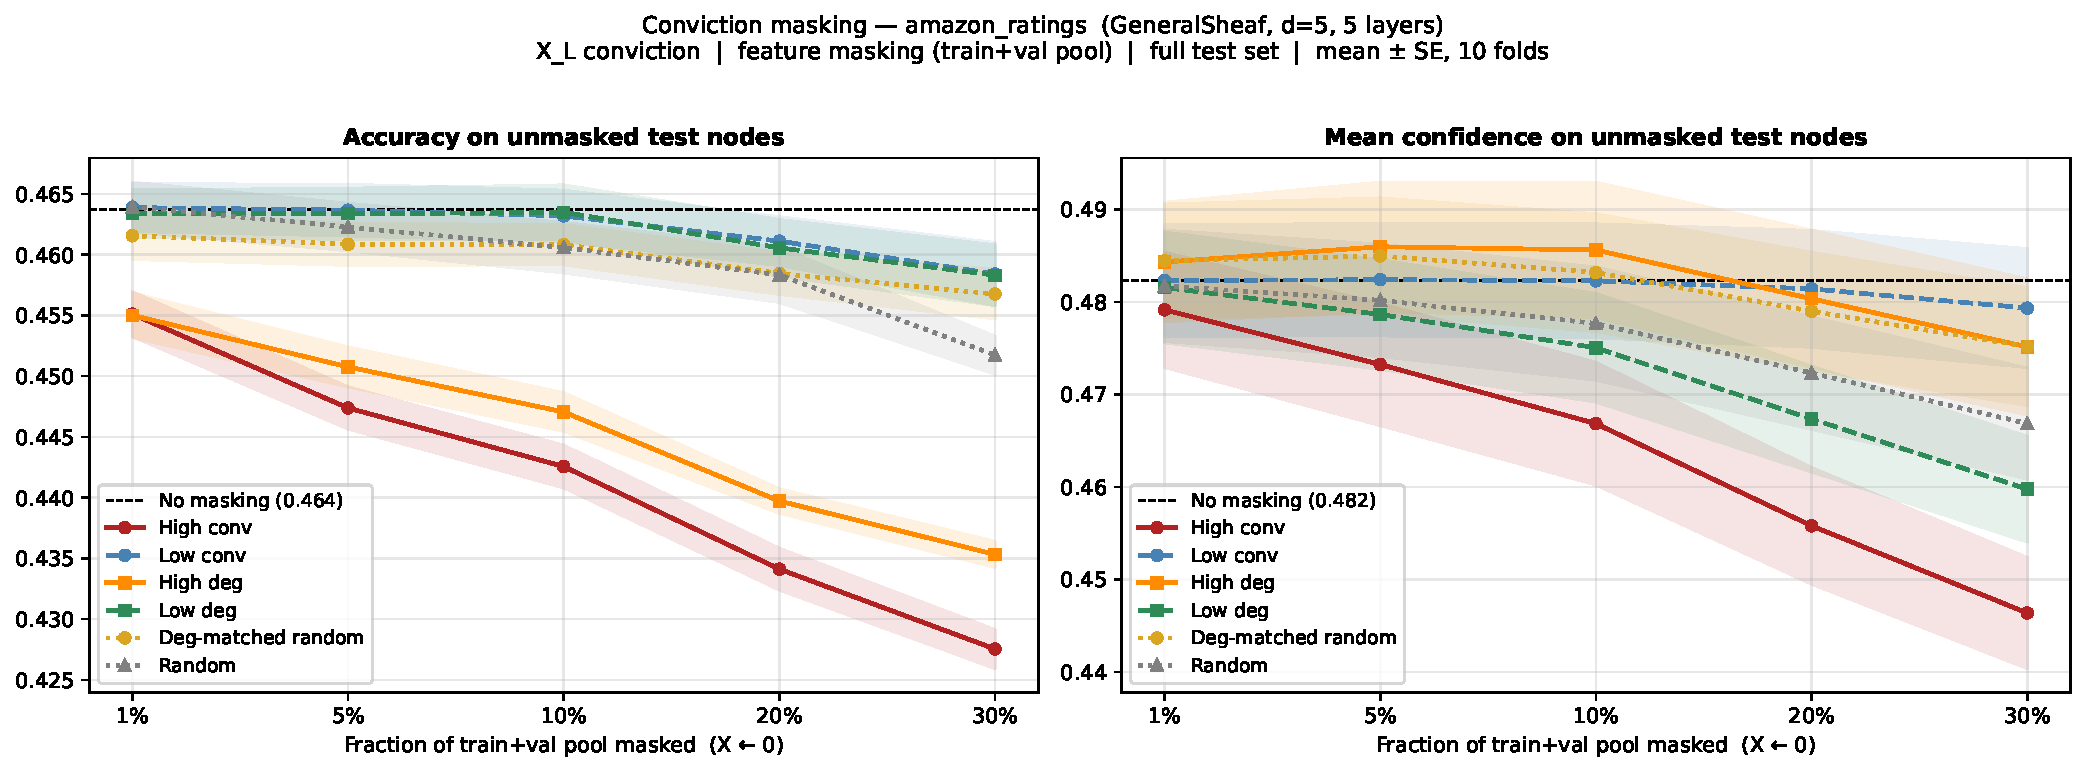
\includegraphics[width=\linewidth]{accuracy_ranking/GeneralSheaf/normalised_true/amazon_ratings_GeneralSheaf_d5_5L_Norm_True_conviction_masking.pdf}
\end{figure}
\end{frame}

\begin{frame}{Citeseer --- GeneralSheaf, $d=5$, $L=4$, Norm=True}
\begin{figure}
    \centering
    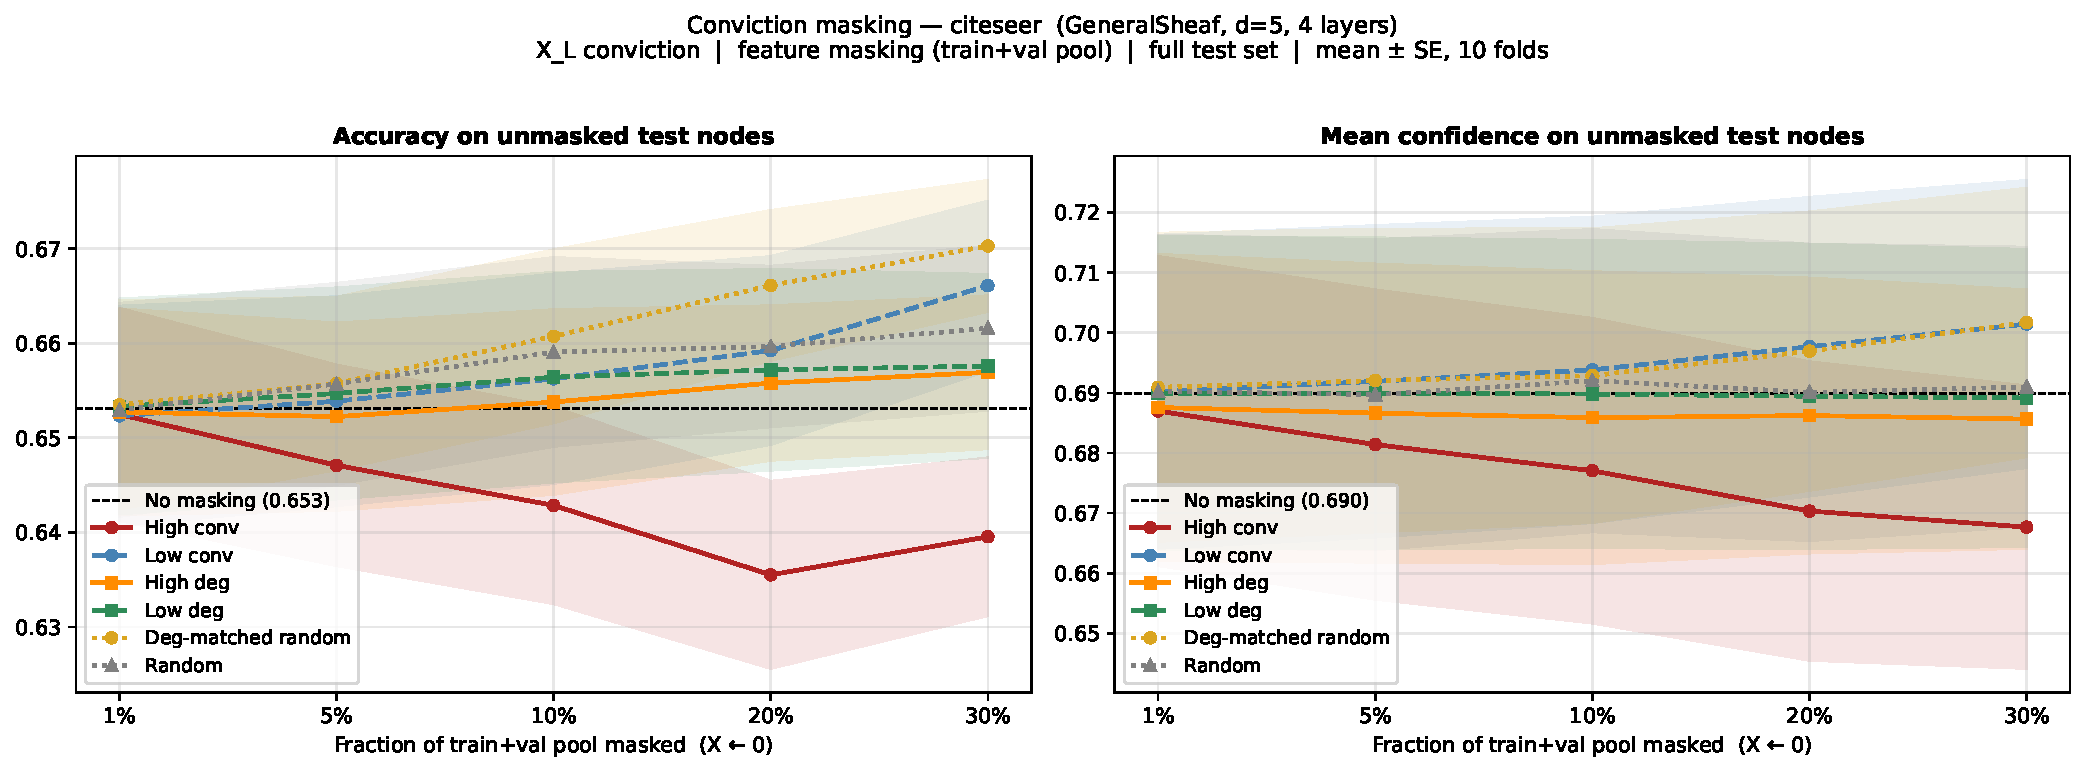
\includegraphics[width=\linewidth]{accuracy_ranking/GeneralSheaf/normalised_true/citeseer_GeneralSheaf_d5_4L_Norm_True_conviction_masking.pdf}
\end{figure}
\end{frame}

\begin{frame}{Cora --- GeneralSheaf, $d=5$, $L=3$, Norm=True}
\begin{figure}
    \centering
    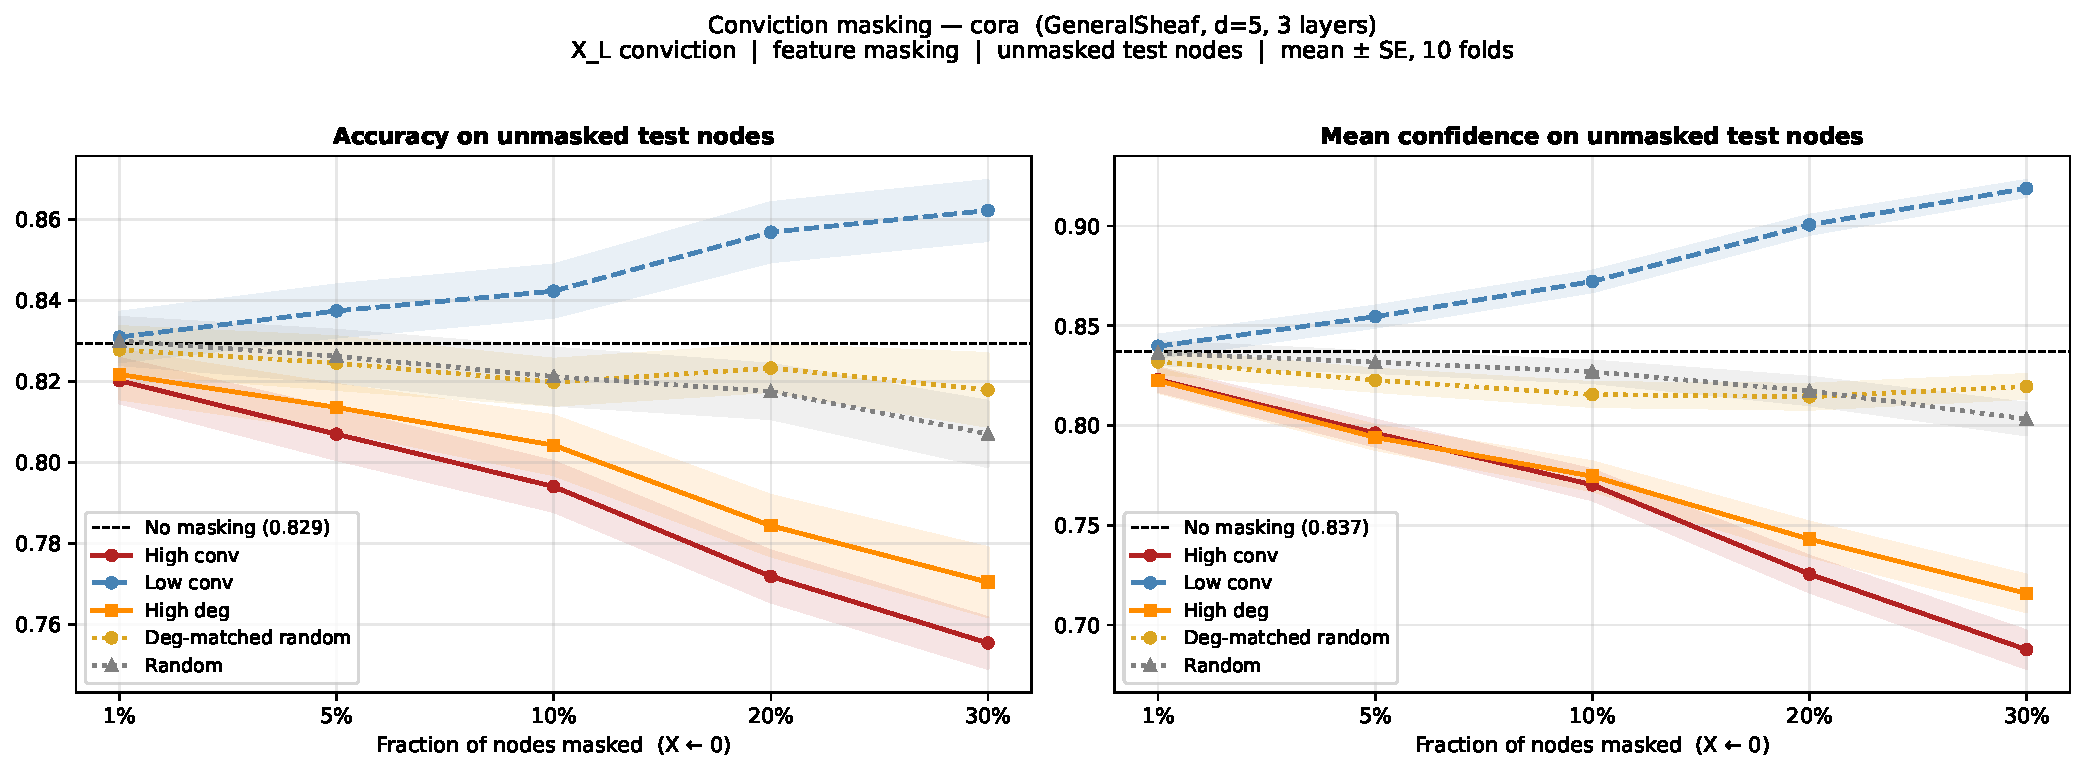
\includegraphics[width=\linewidth]{accuracy_ranking/GeneralSheaf/normalised_true/cora_GeneralSheaf_d5_3L_Norm_True_conviction_masking.pdf}
\end{figure}
\end{frame}

\begin{frame}{Cornell --- GeneralSheaf, $d=2$, $L=2$, Norm=True}
\begin{figure}
    \centering
    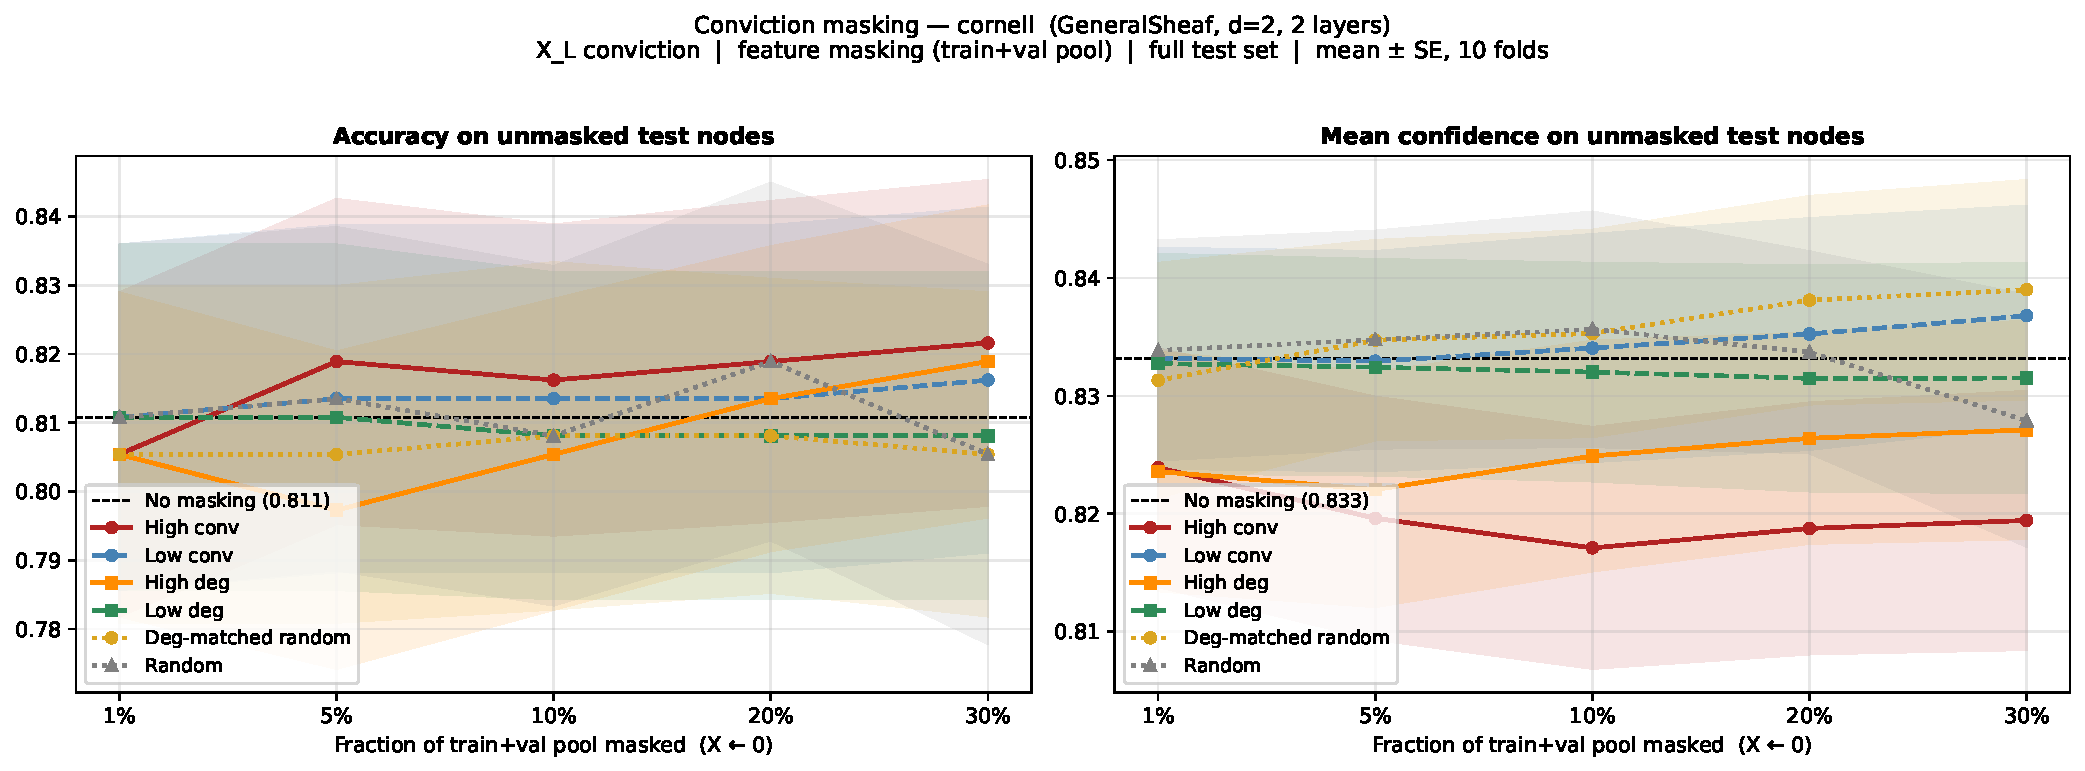
\includegraphics[width=0.8\linewidth]{accuracy_ranking/GeneralSheaf/normalised_true/cornell_GeneralSheaf_d2_2L_Norm_True_conviction_masking.pdf}
\end{figure}
\end{frame}

\begin{frame}{Minesweeper --- GeneralSheaf, $d=5$, $L=6$, Norm=True}
\begin{figure}
    \centering
    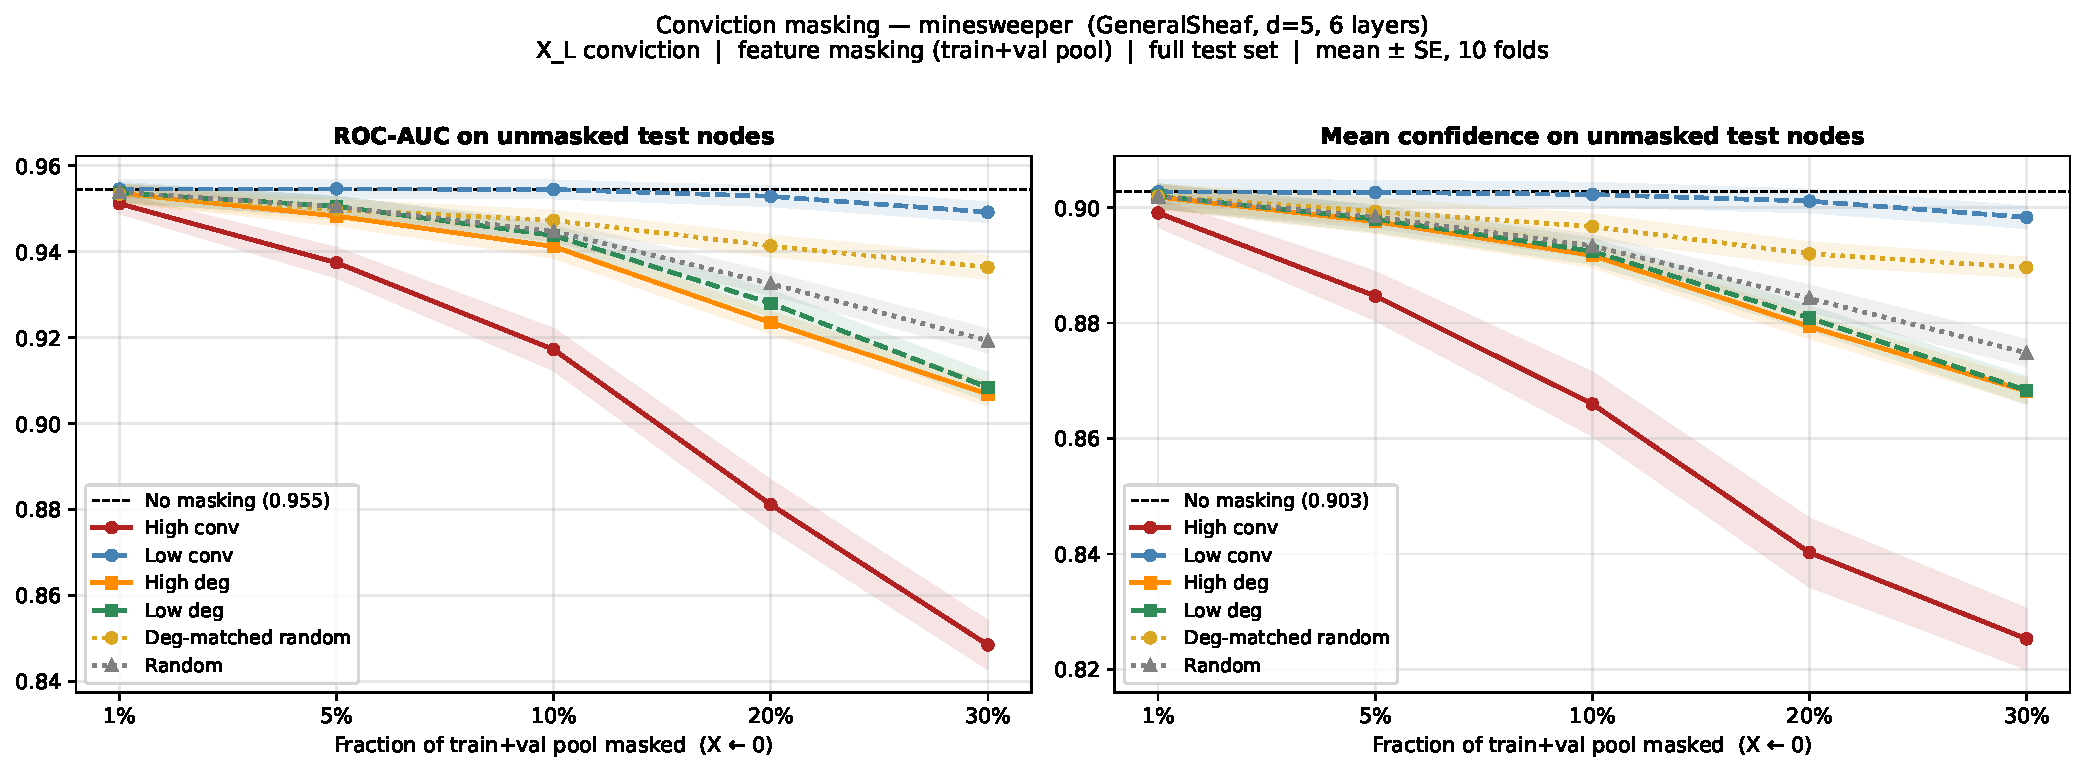
\includegraphics[width=\linewidth]{accuracy_ranking/GeneralSheaf/normalised_true/minesweeper_GeneralSheaf_d5_6L_Norm_True_conviction_masking.pdf}
\end{figure}
\end{frame}

\begin{frame}{Pubmed --- GeneralSheaf, $d=3$, $L=4$, Norm=True}
\begin{figure}
    \centering
    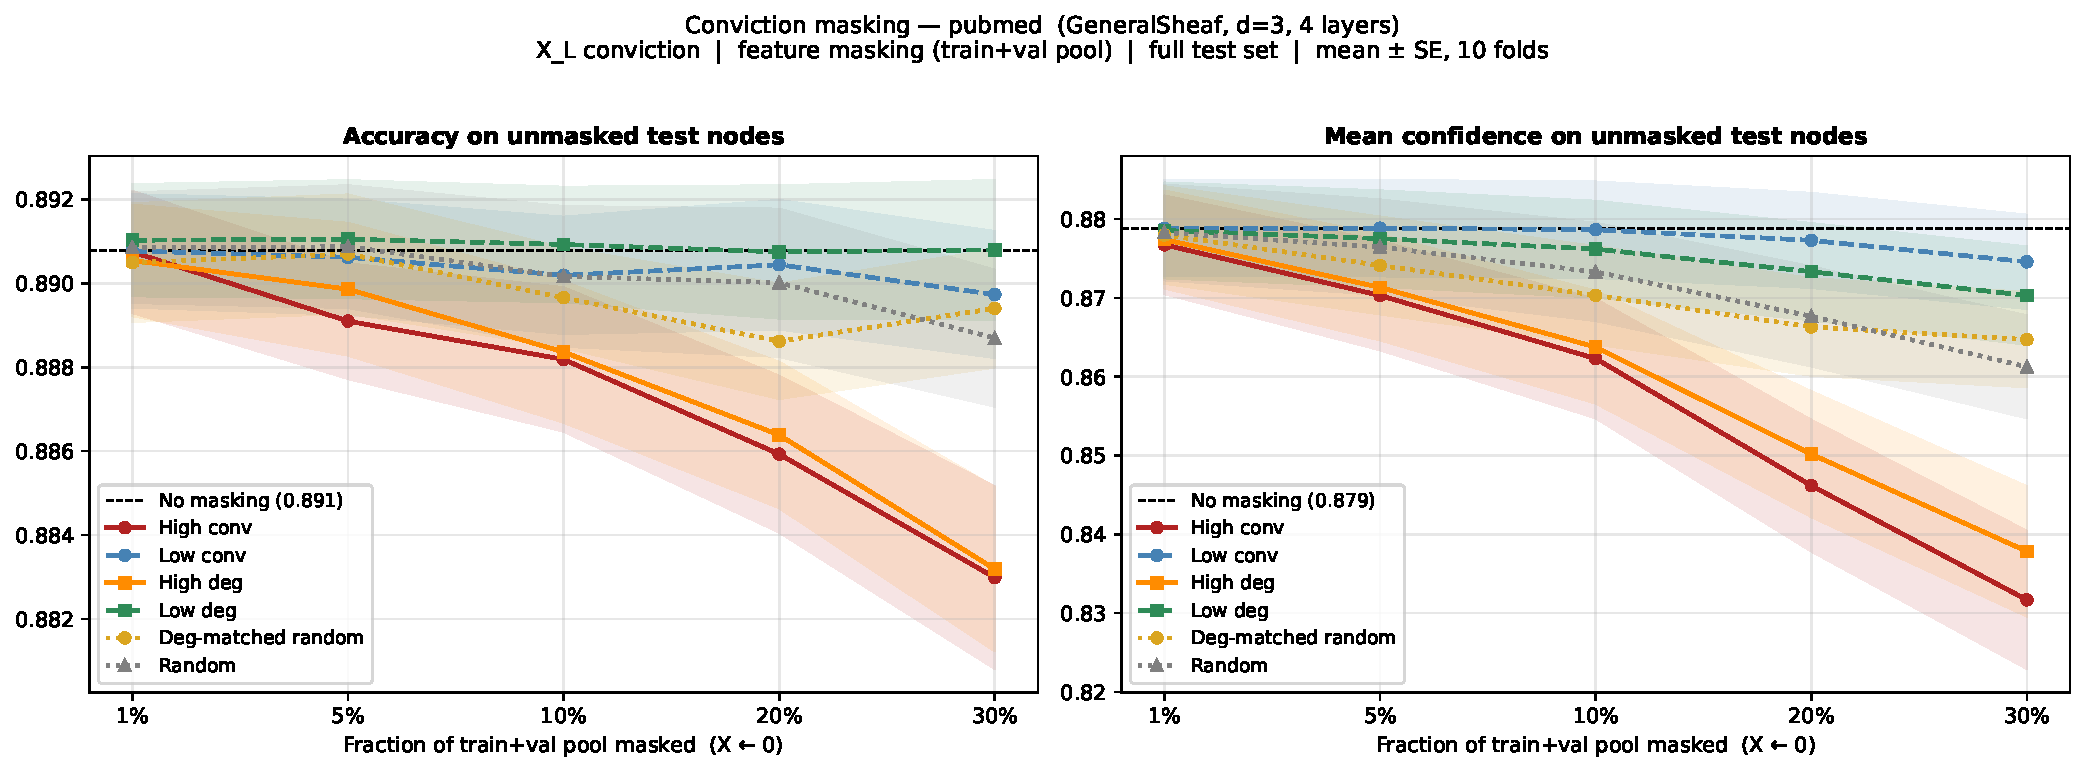
\includegraphics[width=\linewidth]{accuracy_ranking/GeneralSheaf/normalised_true/pubmed_GeneralSheaf_d3_4L_Norm_True_conviction_masking.pdf}
\end{figure}
\end{frame}

\begin{frame}{Questions --- GeneralSheaf, $d=5$, $L=4$, Norm=True}
\begin{figure}
    \centering
    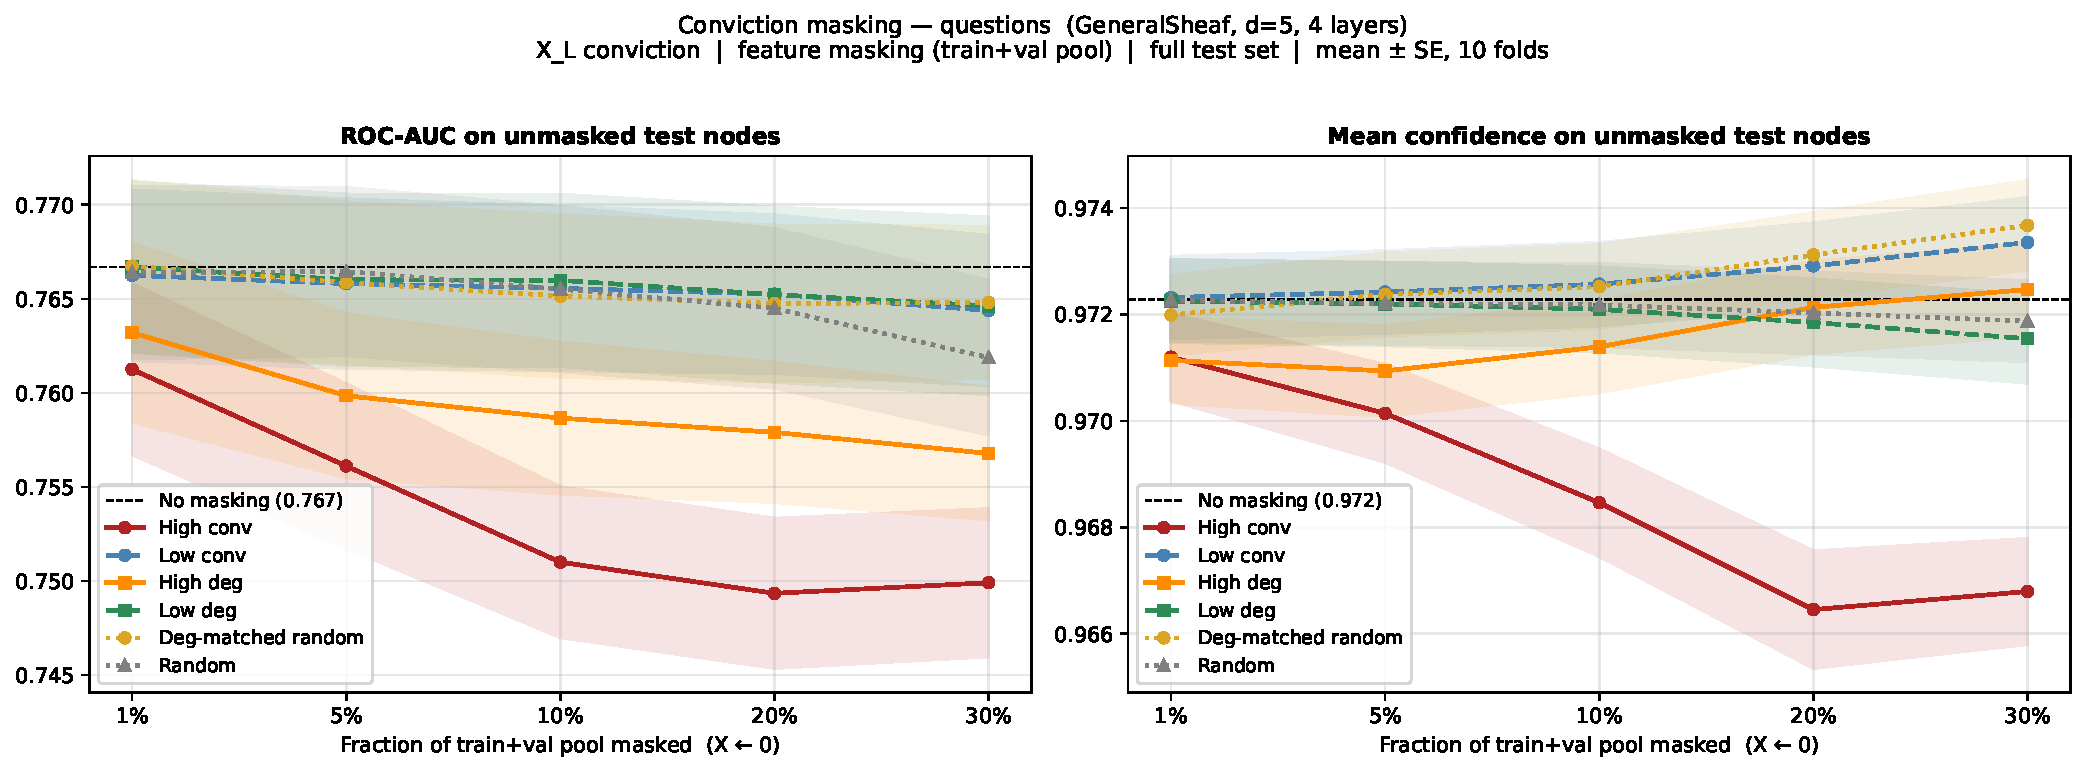
\includegraphics[width=\linewidth]{accuracy_ranking/GeneralSheaf/normalised_true/questions_GeneralSheaf_d5_4L_Norm_True_conviction_masking.pdf}
\end{figure}
\end{frame}

\begin{frame}{Roman Empire --- GeneralSheaf, $d=5$, $L=5$, Norm=True}
\begin{figure}
    \centering
    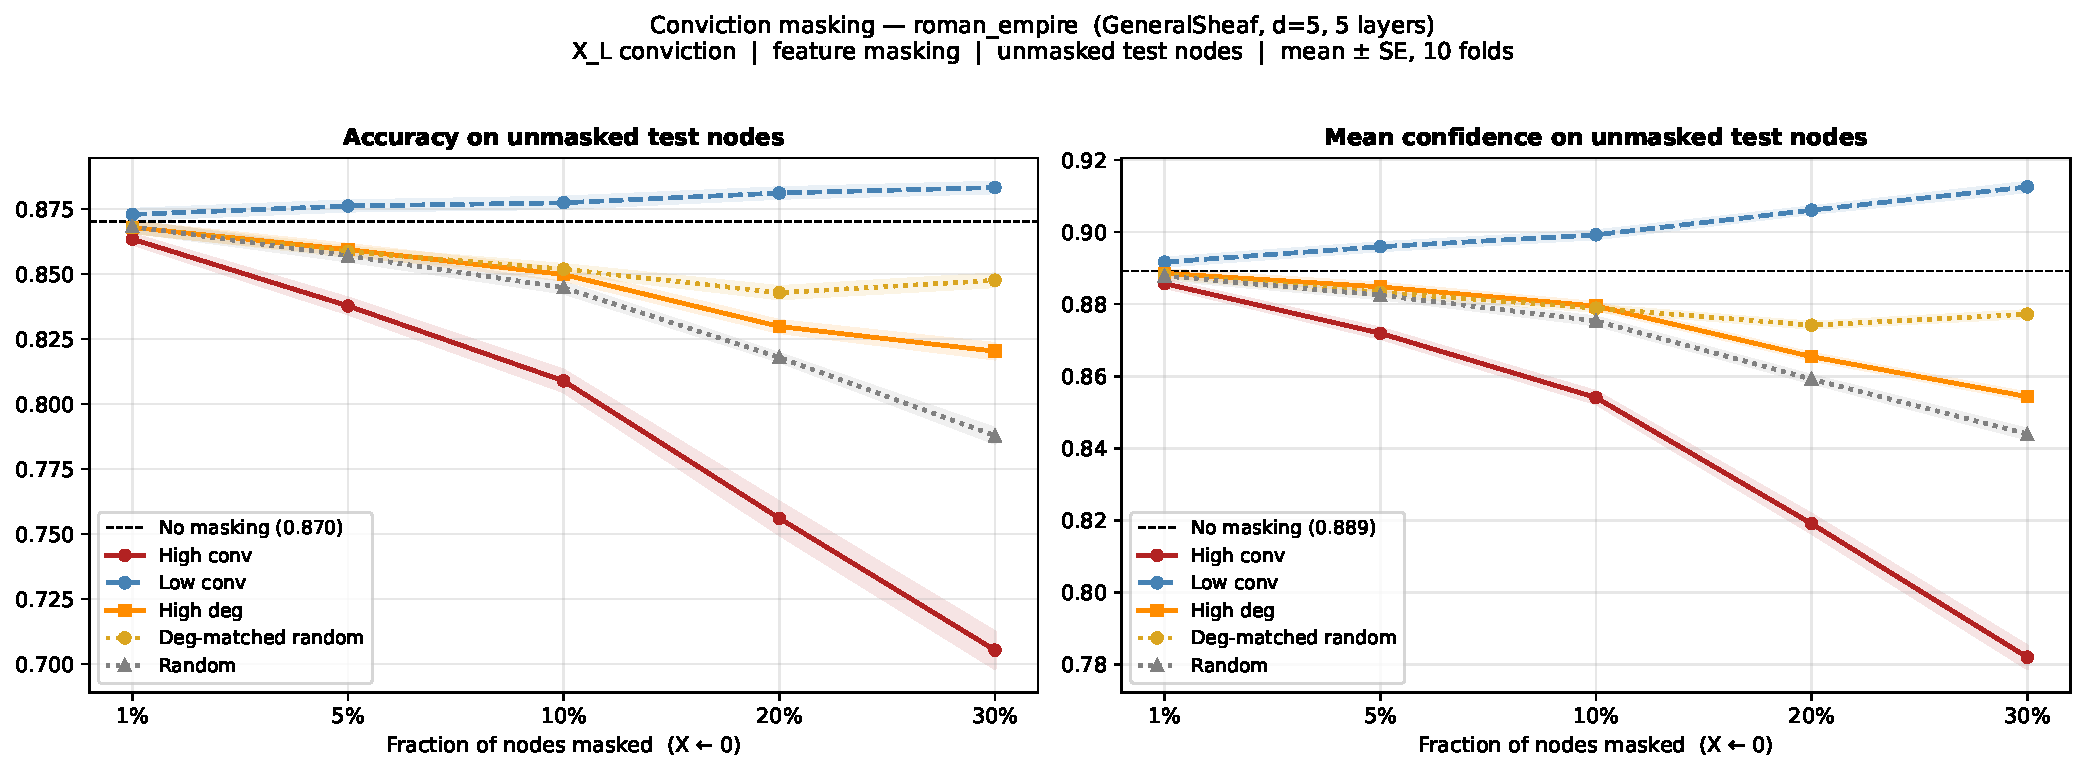
\includegraphics[width=\linewidth]{accuracy_ranking/GeneralSheaf/normalised_true/roman_empire_GeneralSheaf_d5_5L_Norm_True_conviction_masking.pdf}
\end{figure}
\end{frame}

\begin{frame}{Tolokers --- GeneralSheaf, $d=3$, $L=4$, Norm=True}
\begin{figure}
    \centering
    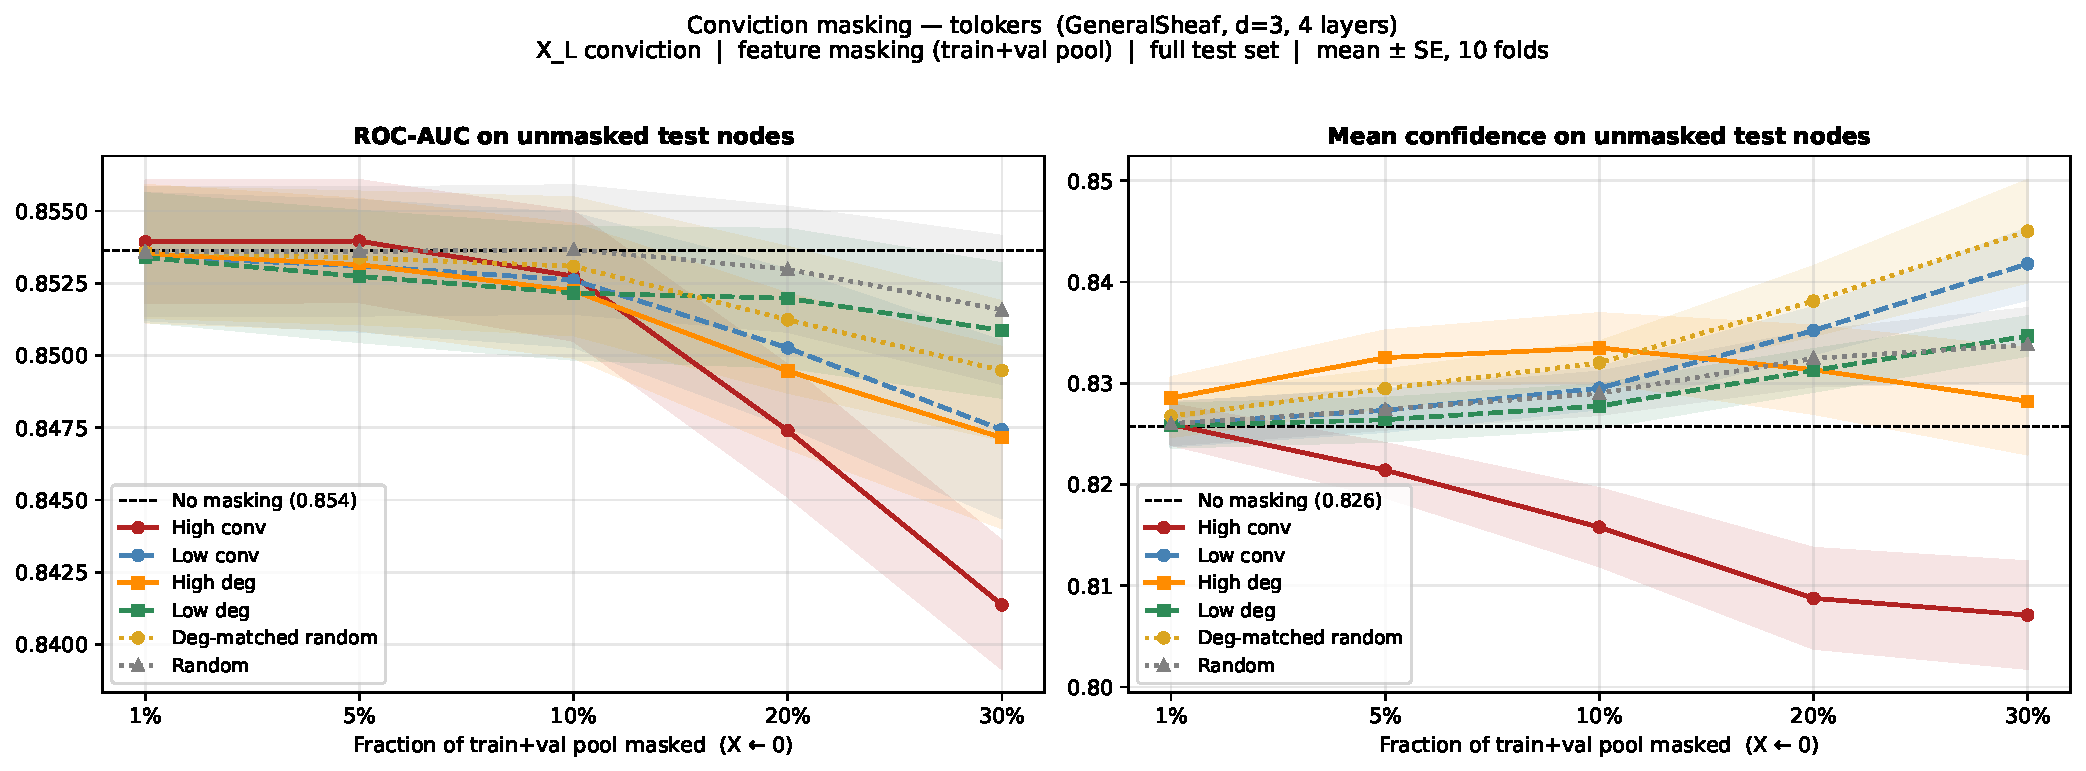
\includegraphics[width=\linewidth]{accuracy_ranking/GeneralSheaf/normalised_true/tolokers_GeneralSheaf_d3_4L_Norm_True_conviction_masking.pdf}
\end{figure}
\end{frame}

\begin{frame}{Wisconsin --- GeneralSheaf, $d=2$, $L=2$, Norm=True}
\begin{figure}
    \centering
    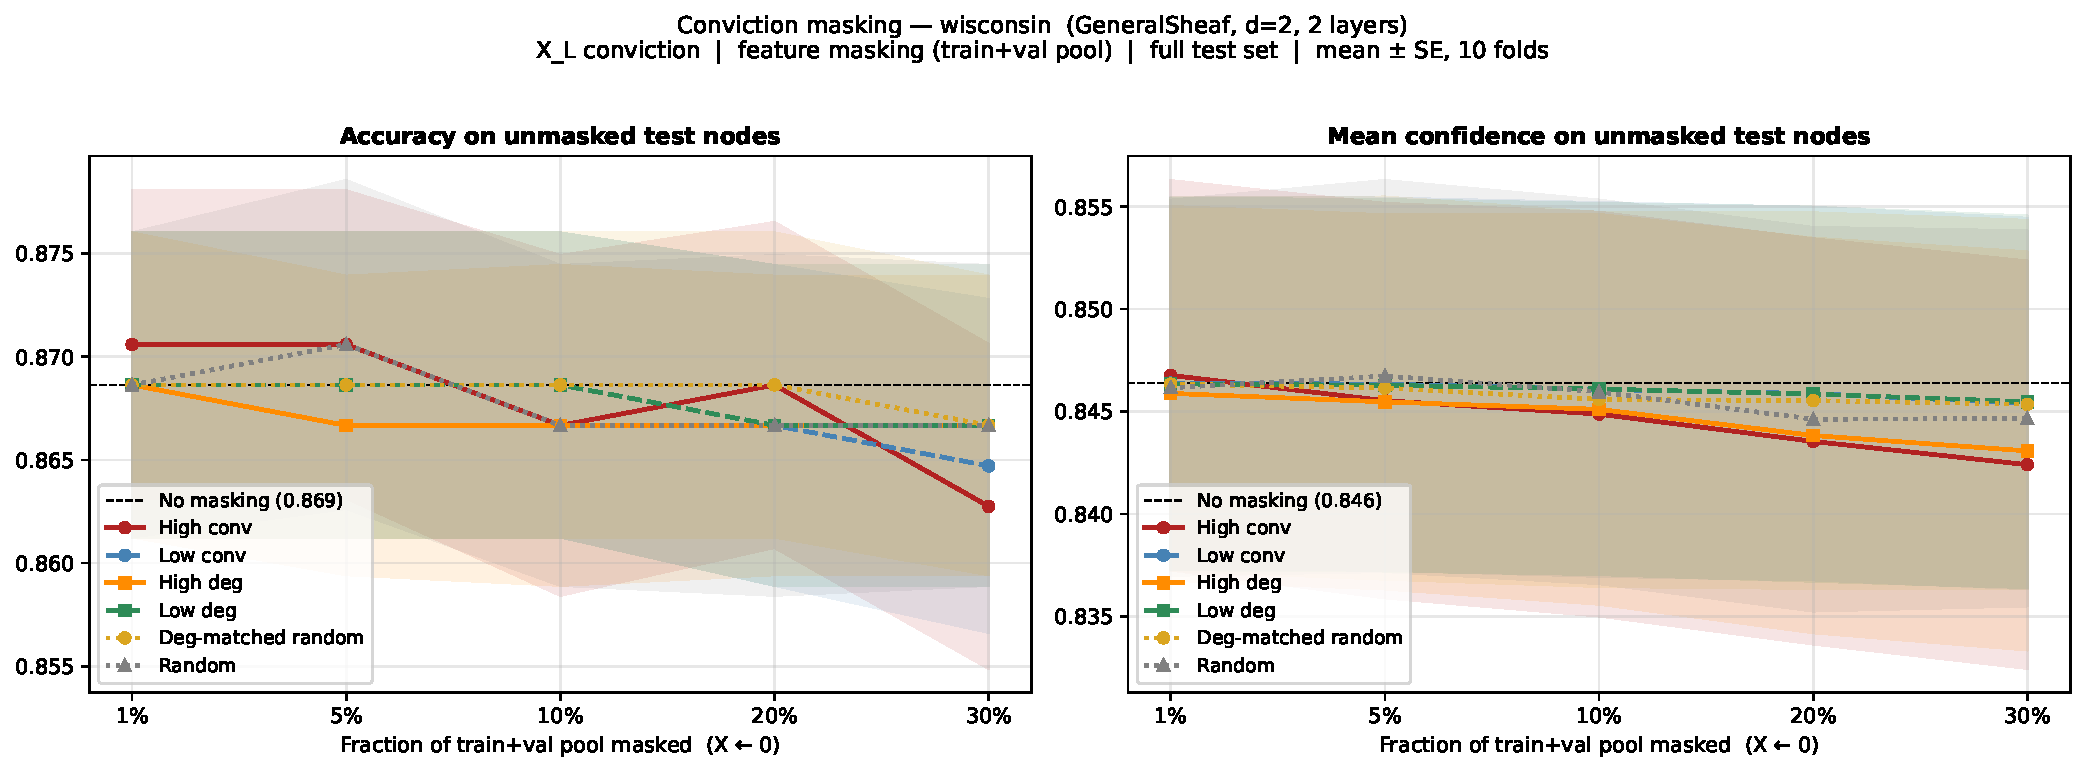
\includegraphics[width=0.8\linewidth]{accuracy_ranking/GeneralSheaf/normalised_true/wisconsin_GeneralSheaf_d2_2L_Norm_True_conviction_masking.pdf}
\end{figure}
\end{frame}




% ══════════════════════════════════════════════════════════════════════════════
%  SECTION 2 — Heatmap, GeneralSheaf, normalised=True
% ══════════════════════════════════════════════════════════════════════════════

\begin{frame}{}
\centering
\Huge\textbf{Conviction Heatmap}\\[6pt]
\Large GeneralSheaf \quad (\texttt{normalised=True})
\end{frame}

\begin{frame}{Amazon Ratings --- GeneralSheaf, $d=5$, $L=5$, Norm=True}
\begin{figure}
    \centering
    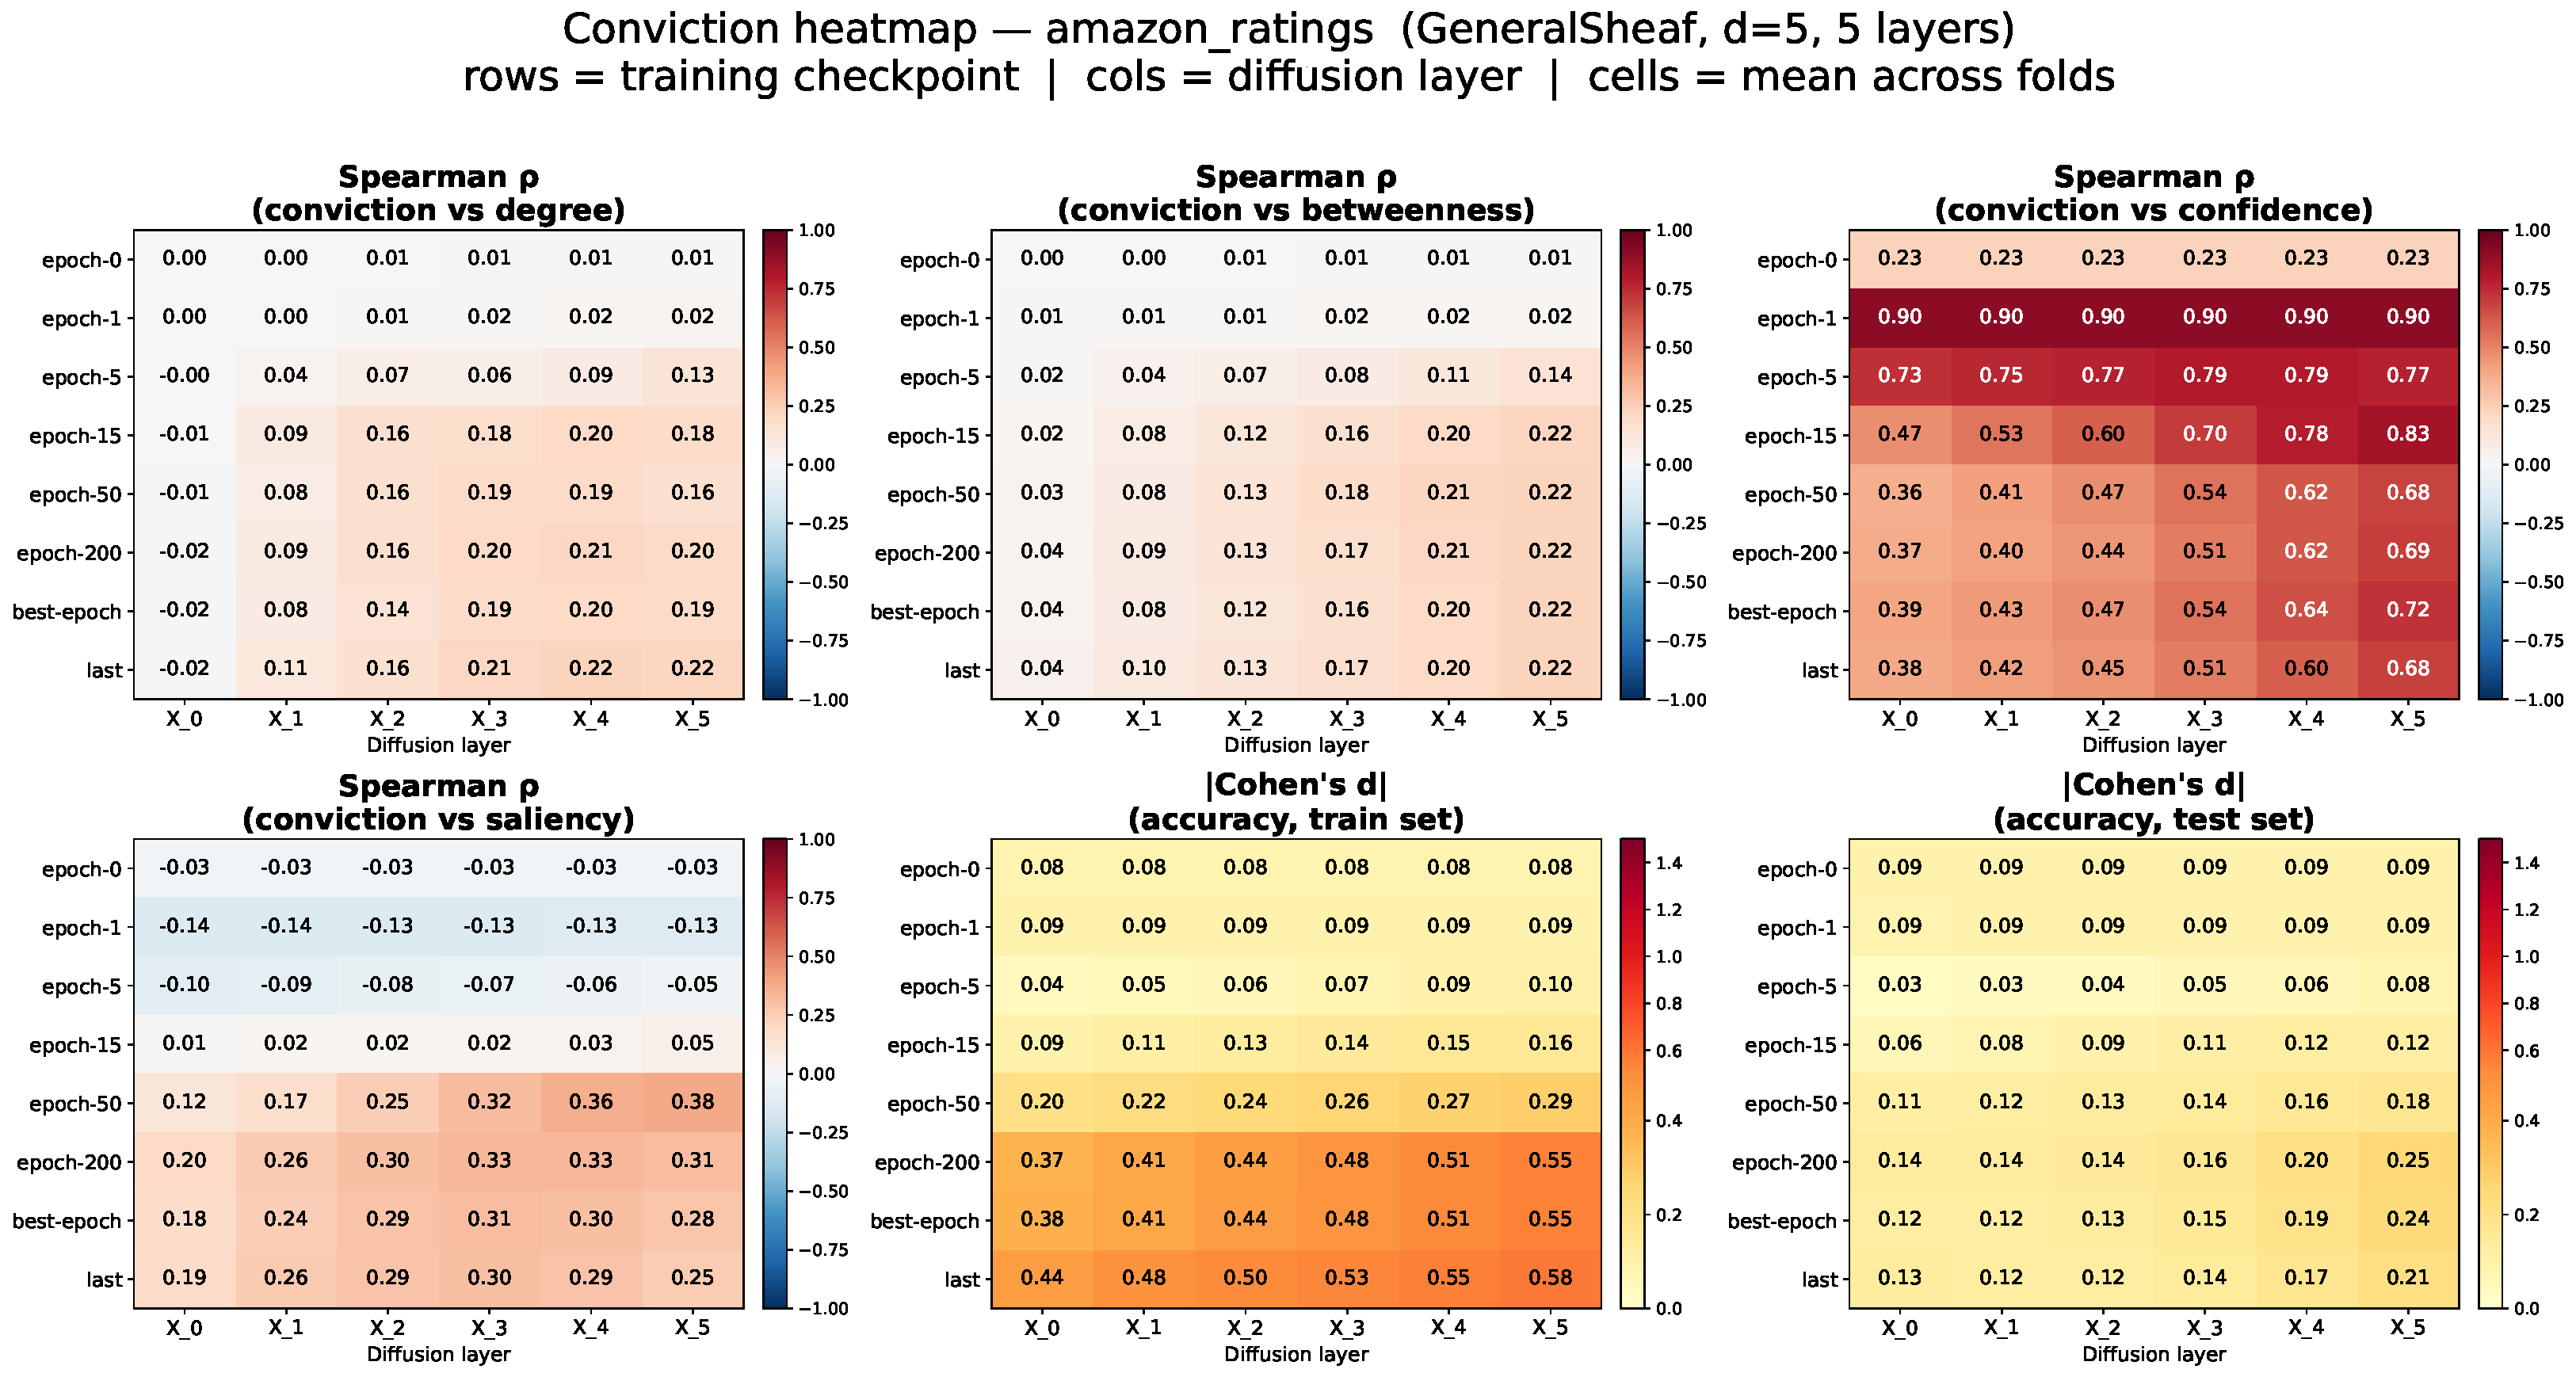
\includegraphics[width=\linewidth]{conviction_heatmap/GeneralSheaf/normalised_true/amazon_ratings_GeneralSheaf_d5_5L_Norm_True_conviction_heatmap.pdf}
\end{figure}
\end{frame}

\begin{frame}{Citeseer --- GeneralSheaf, $d=5$, $L=4$, Norm=True}
\begin{figure}
    \centering
    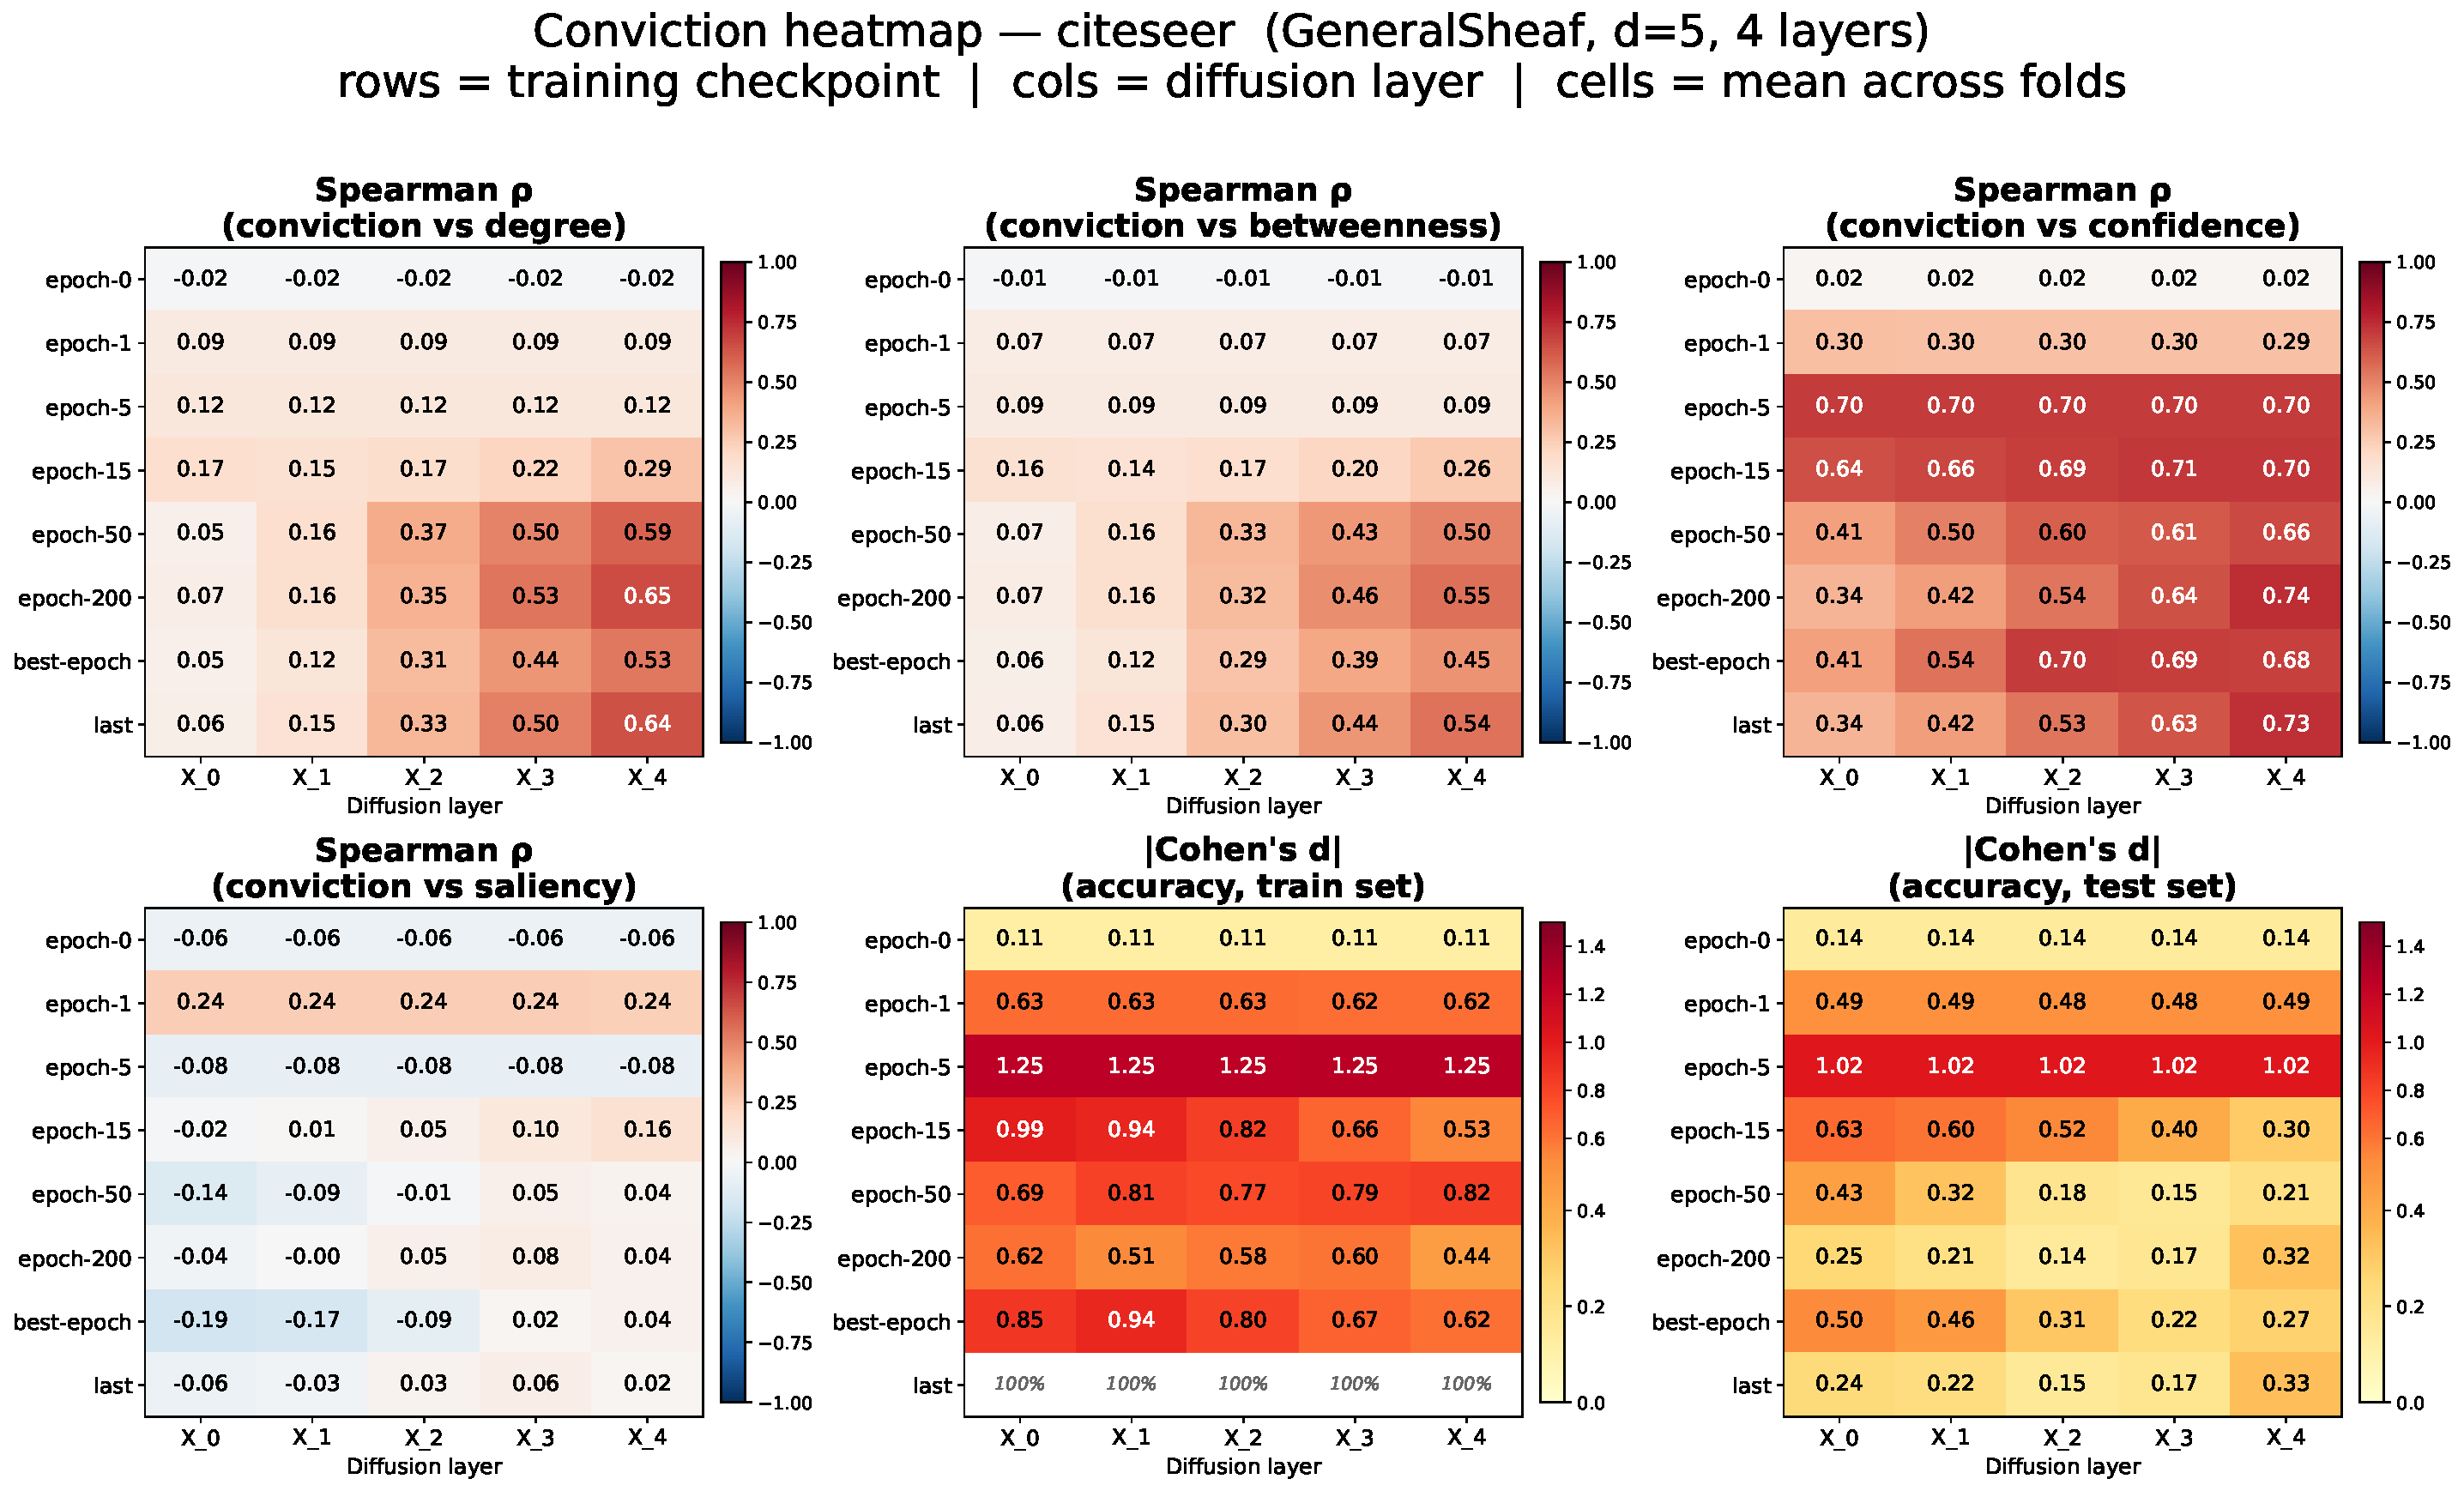
\includegraphics[width=\linewidth]{conviction_heatmap/GeneralSheaf/normalised_true/citeseer_GeneralSheaf_d5_4L_Norm_True_conviction_heatmap.pdf}
\end{figure}
\end{frame}

\begin{frame}{Cora --- GeneralSheaf, $d=5$, $L=3$, Norm=True}
\begin{figure}
    \centering
    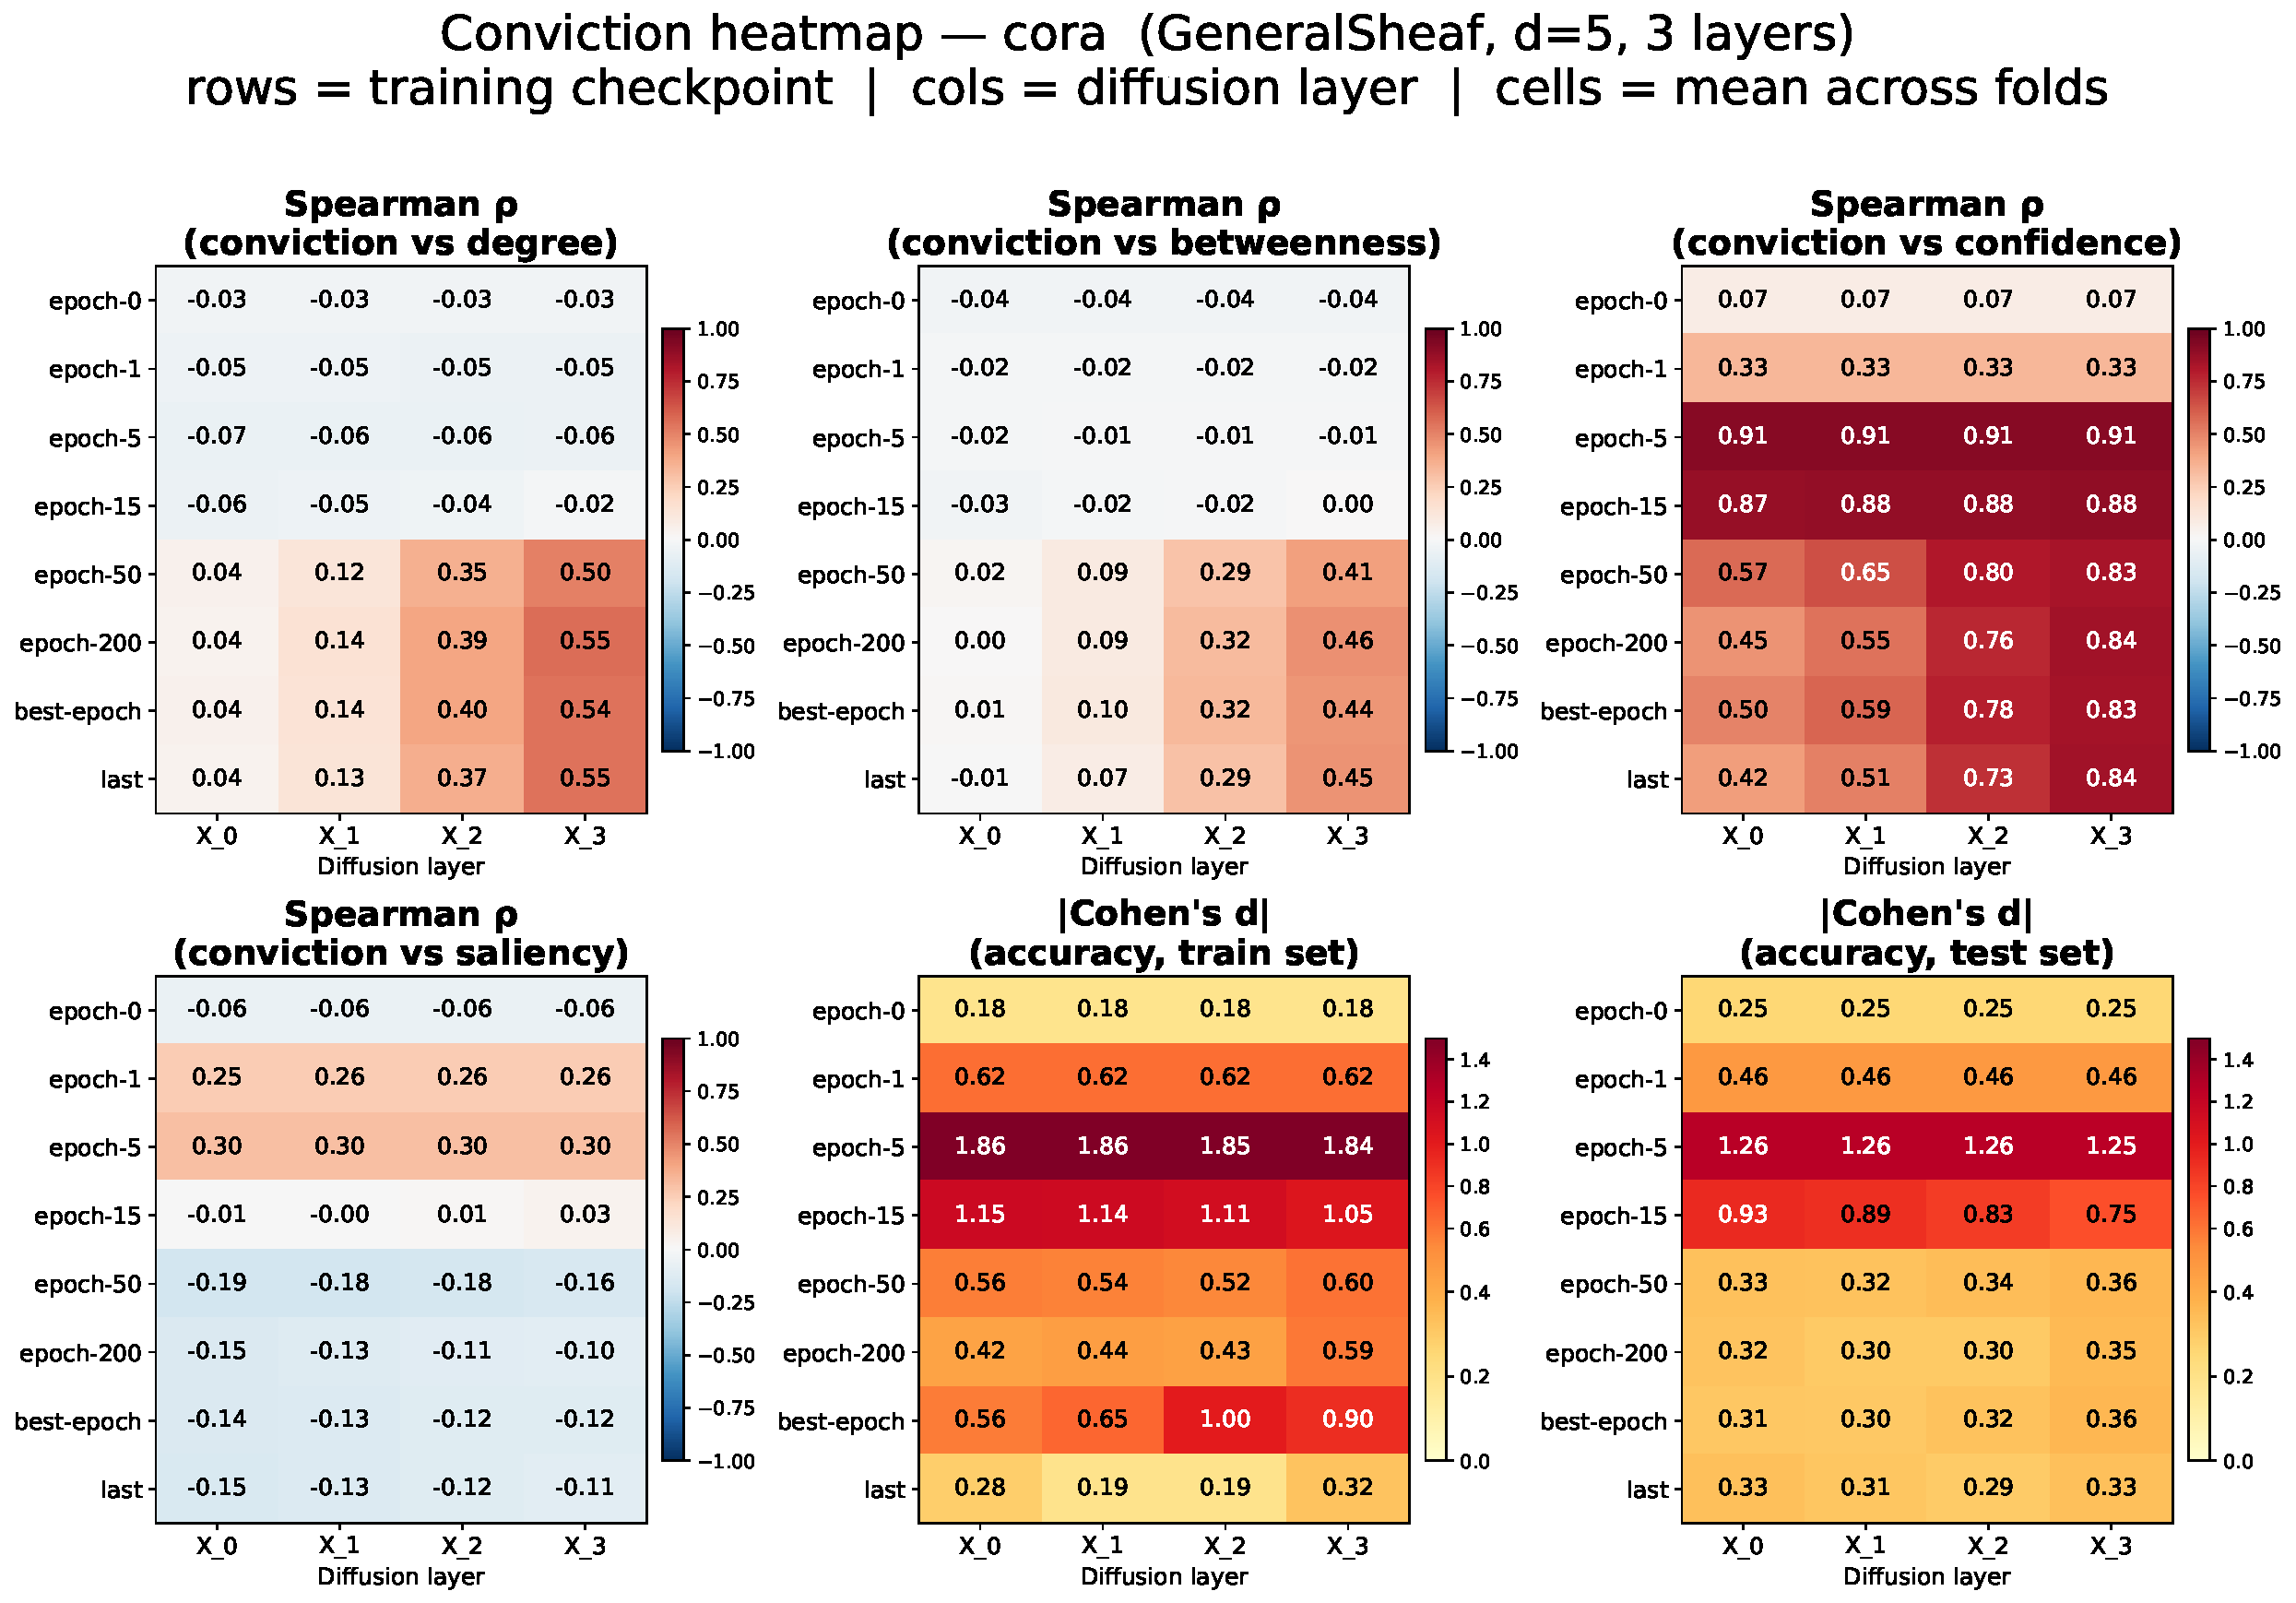
\includegraphics[width=\linewidth]{conviction_heatmap/GeneralSheaf/normalised_true/cora_GeneralSheaf_d5_3L_Norm_True_conviction_heatmap.pdf}
\end{figure}
\end{frame}

\begin{frame}{Cornell --- GeneralSheaf, $d=2$, $L=2$, Norm=True}
\begin{figure}
    \centering
    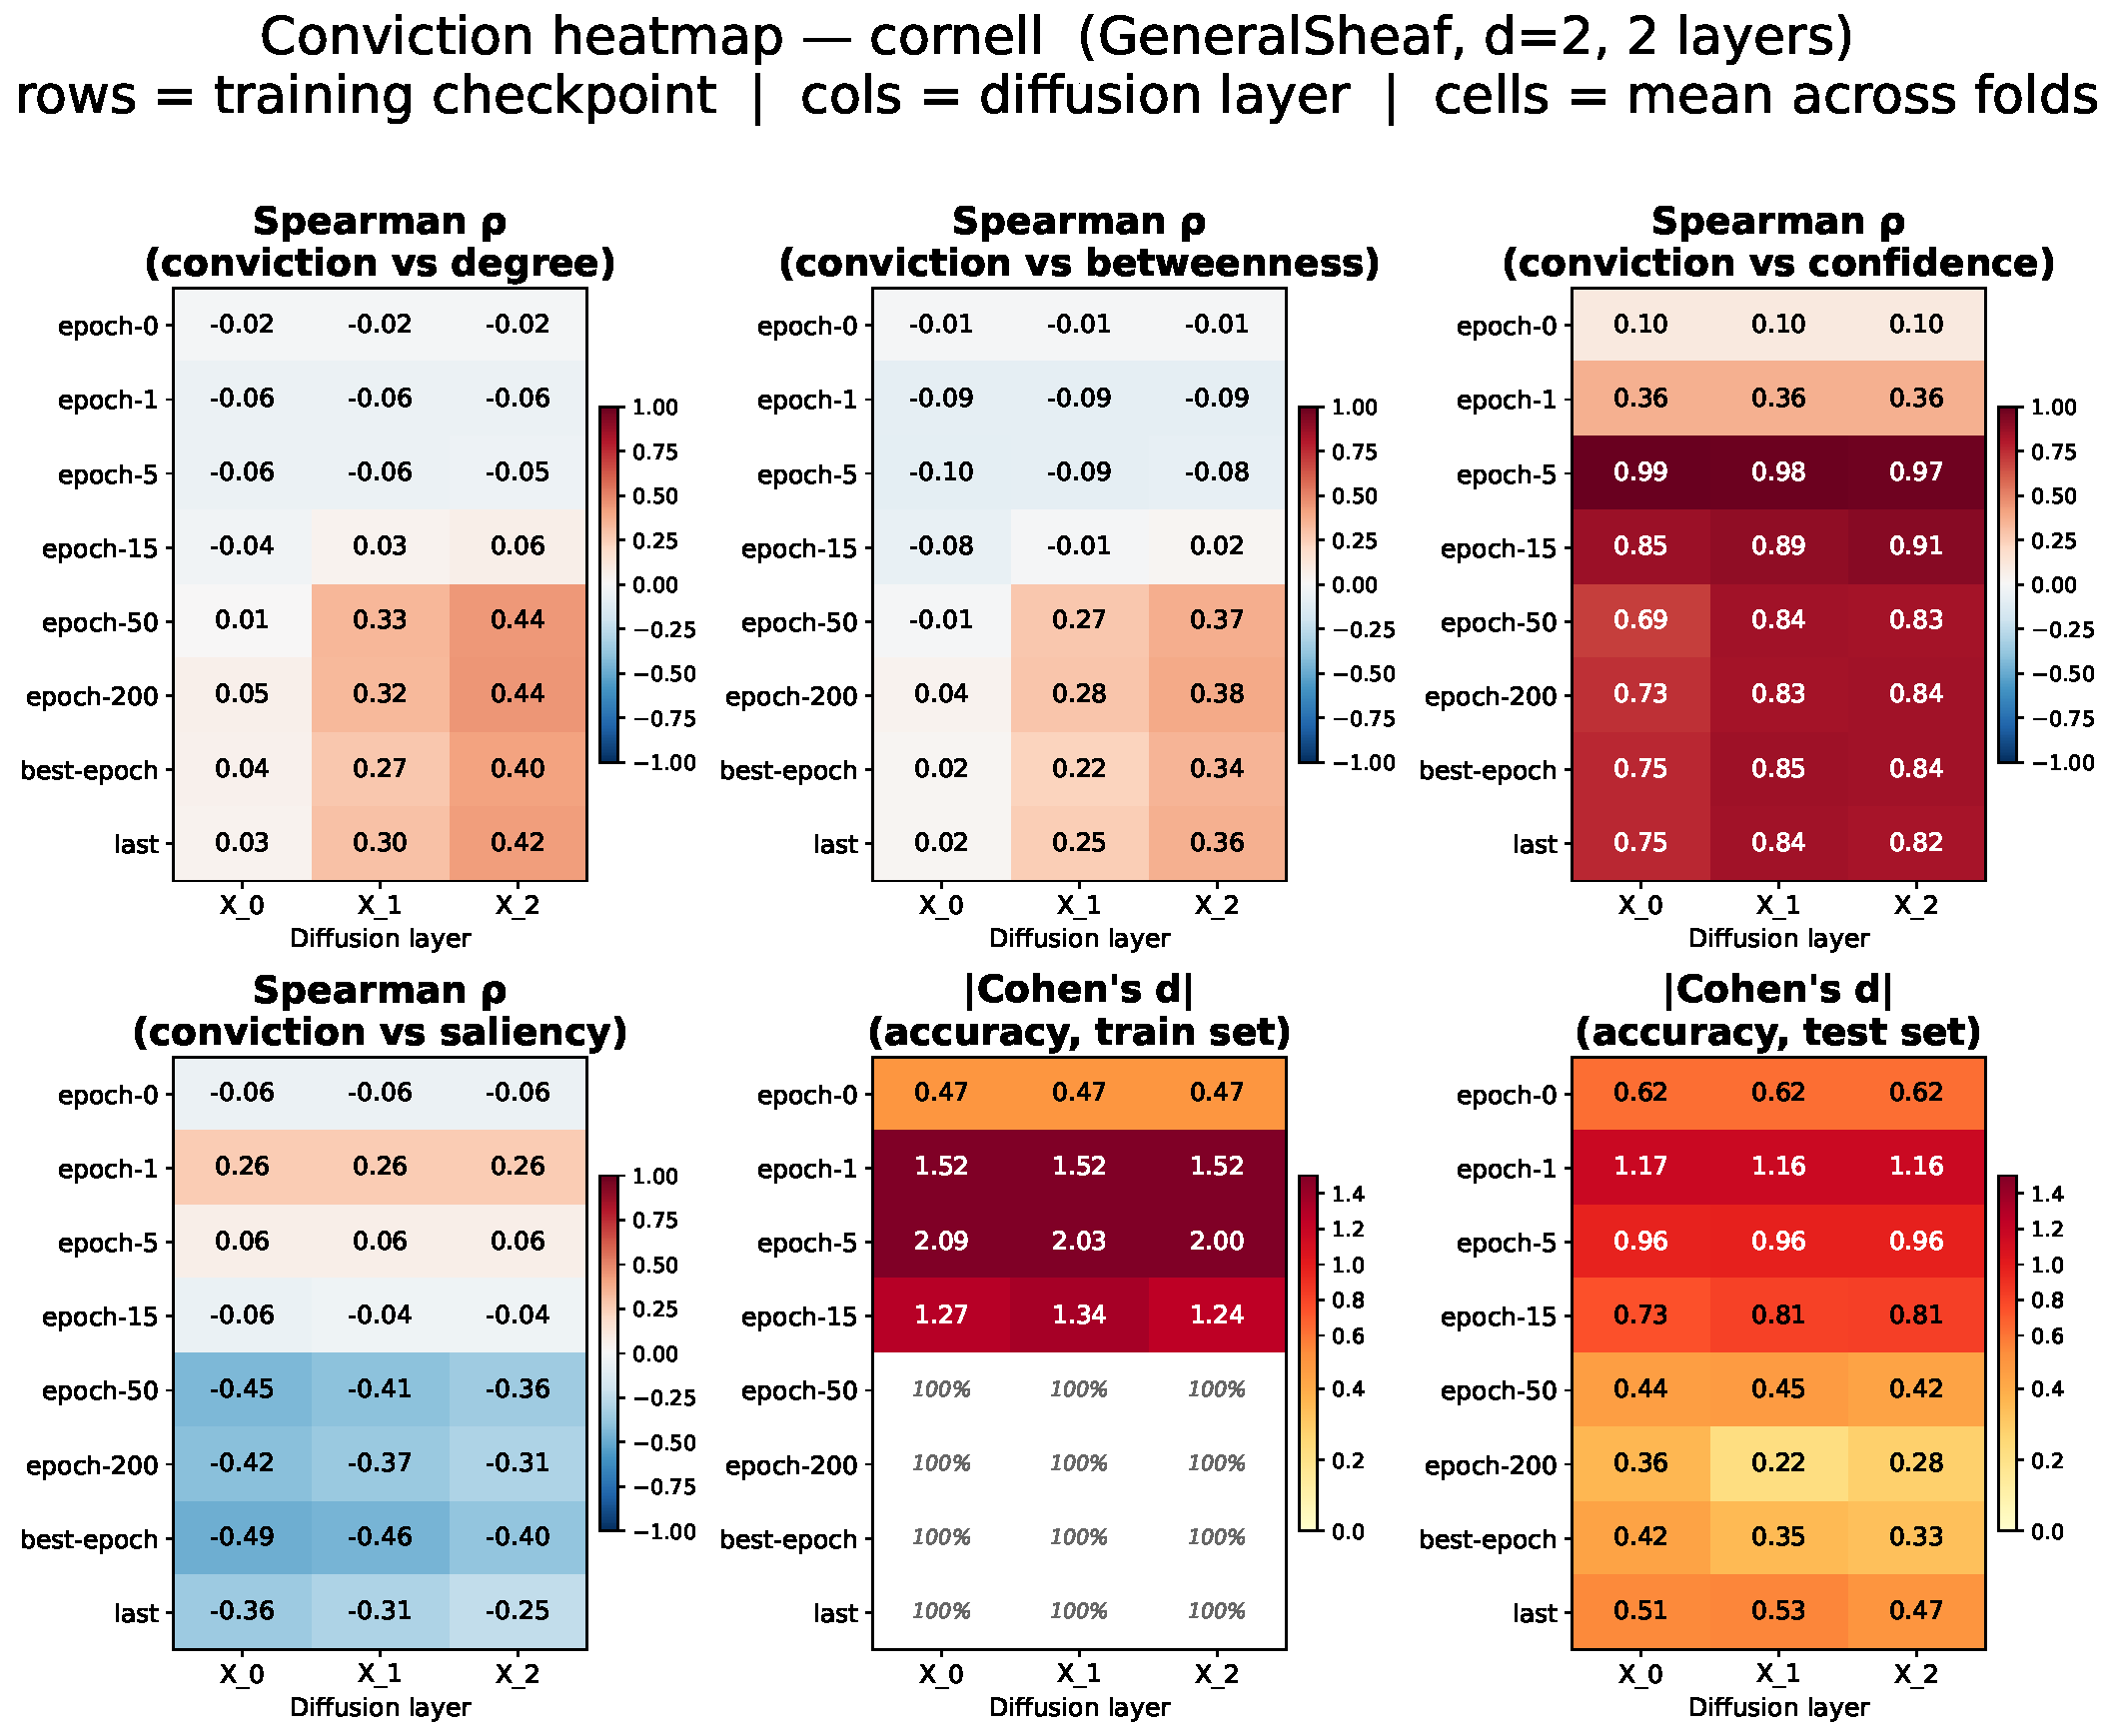
\includegraphics[width=0.8\linewidth]{conviction_heatmap/GeneralSheaf/normalised_true/cornell_GeneralSheaf_d2_2L_Norm_True_conviction_heatmap.pdf}
\end{figure}
\end{frame}

\begin{frame}{Minesweeper --- GeneralSheaf, $d=5$, $L=6$, Norm=True}
\begin{figure}
    \centering
    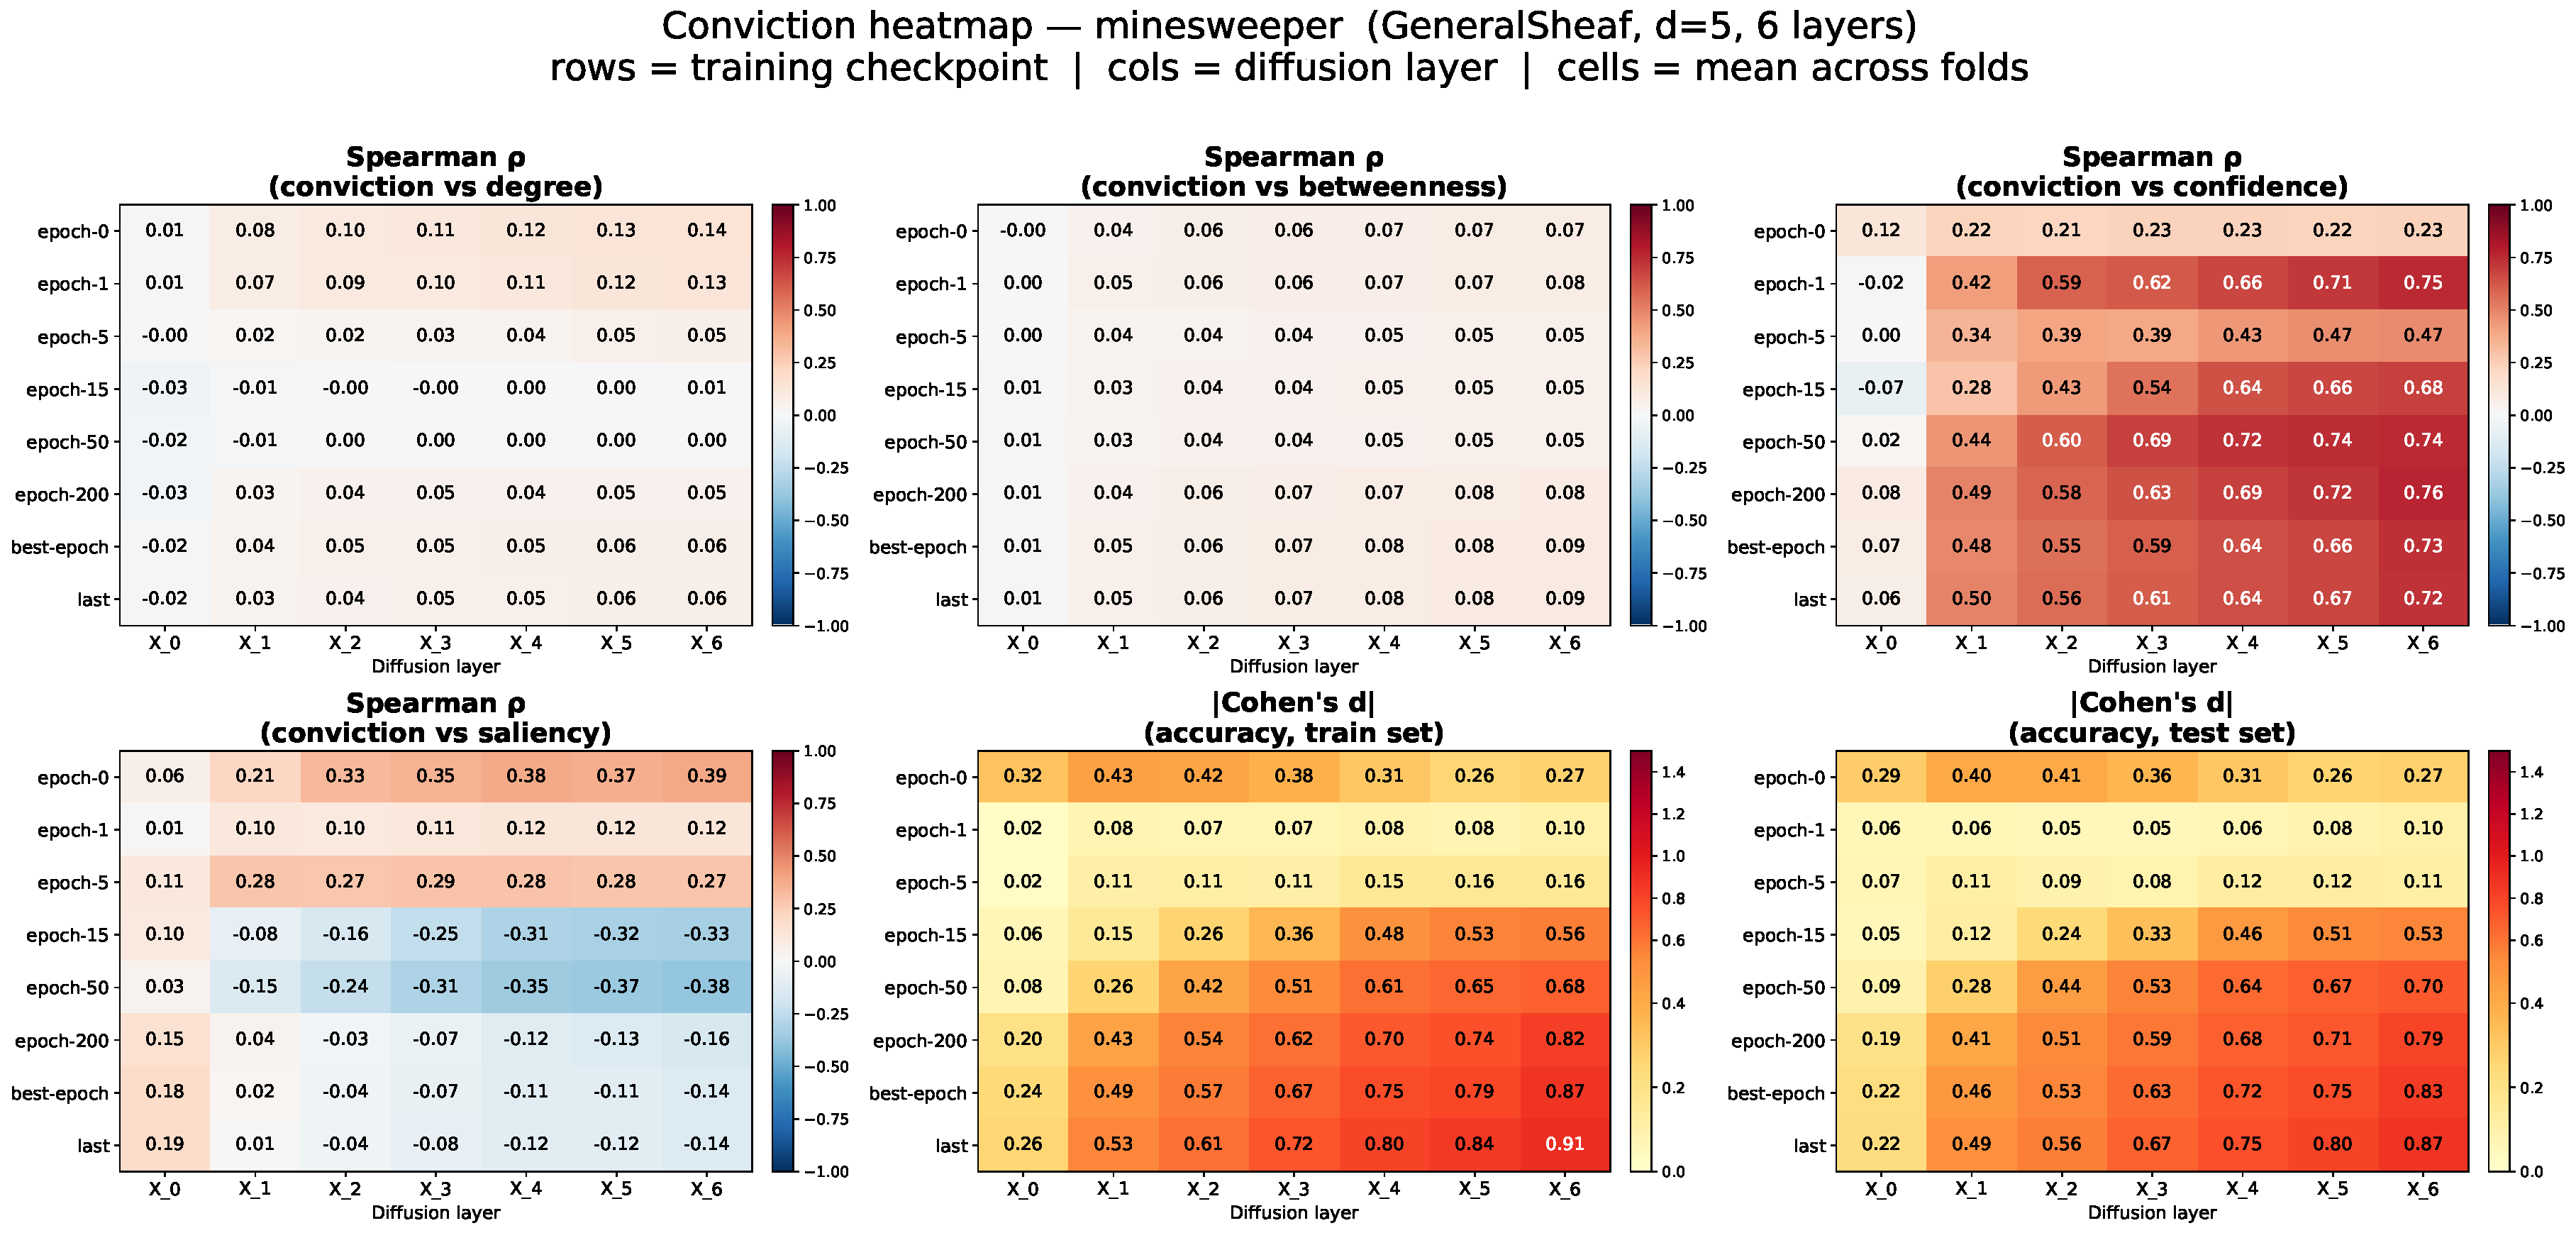
\includegraphics[width=\linewidth]{conviction_heatmap/GeneralSheaf/normalised_true/minesweeper_GeneralSheaf_d5_6L_Norm_True_conviction_heatmap.pdf}
\end{figure}
\end{frame}

\begin{frame}{Pubmed --- GeneralSheaf, $d=3$, $L=4$, Norm=True}
\begin{figure}
    \centering
    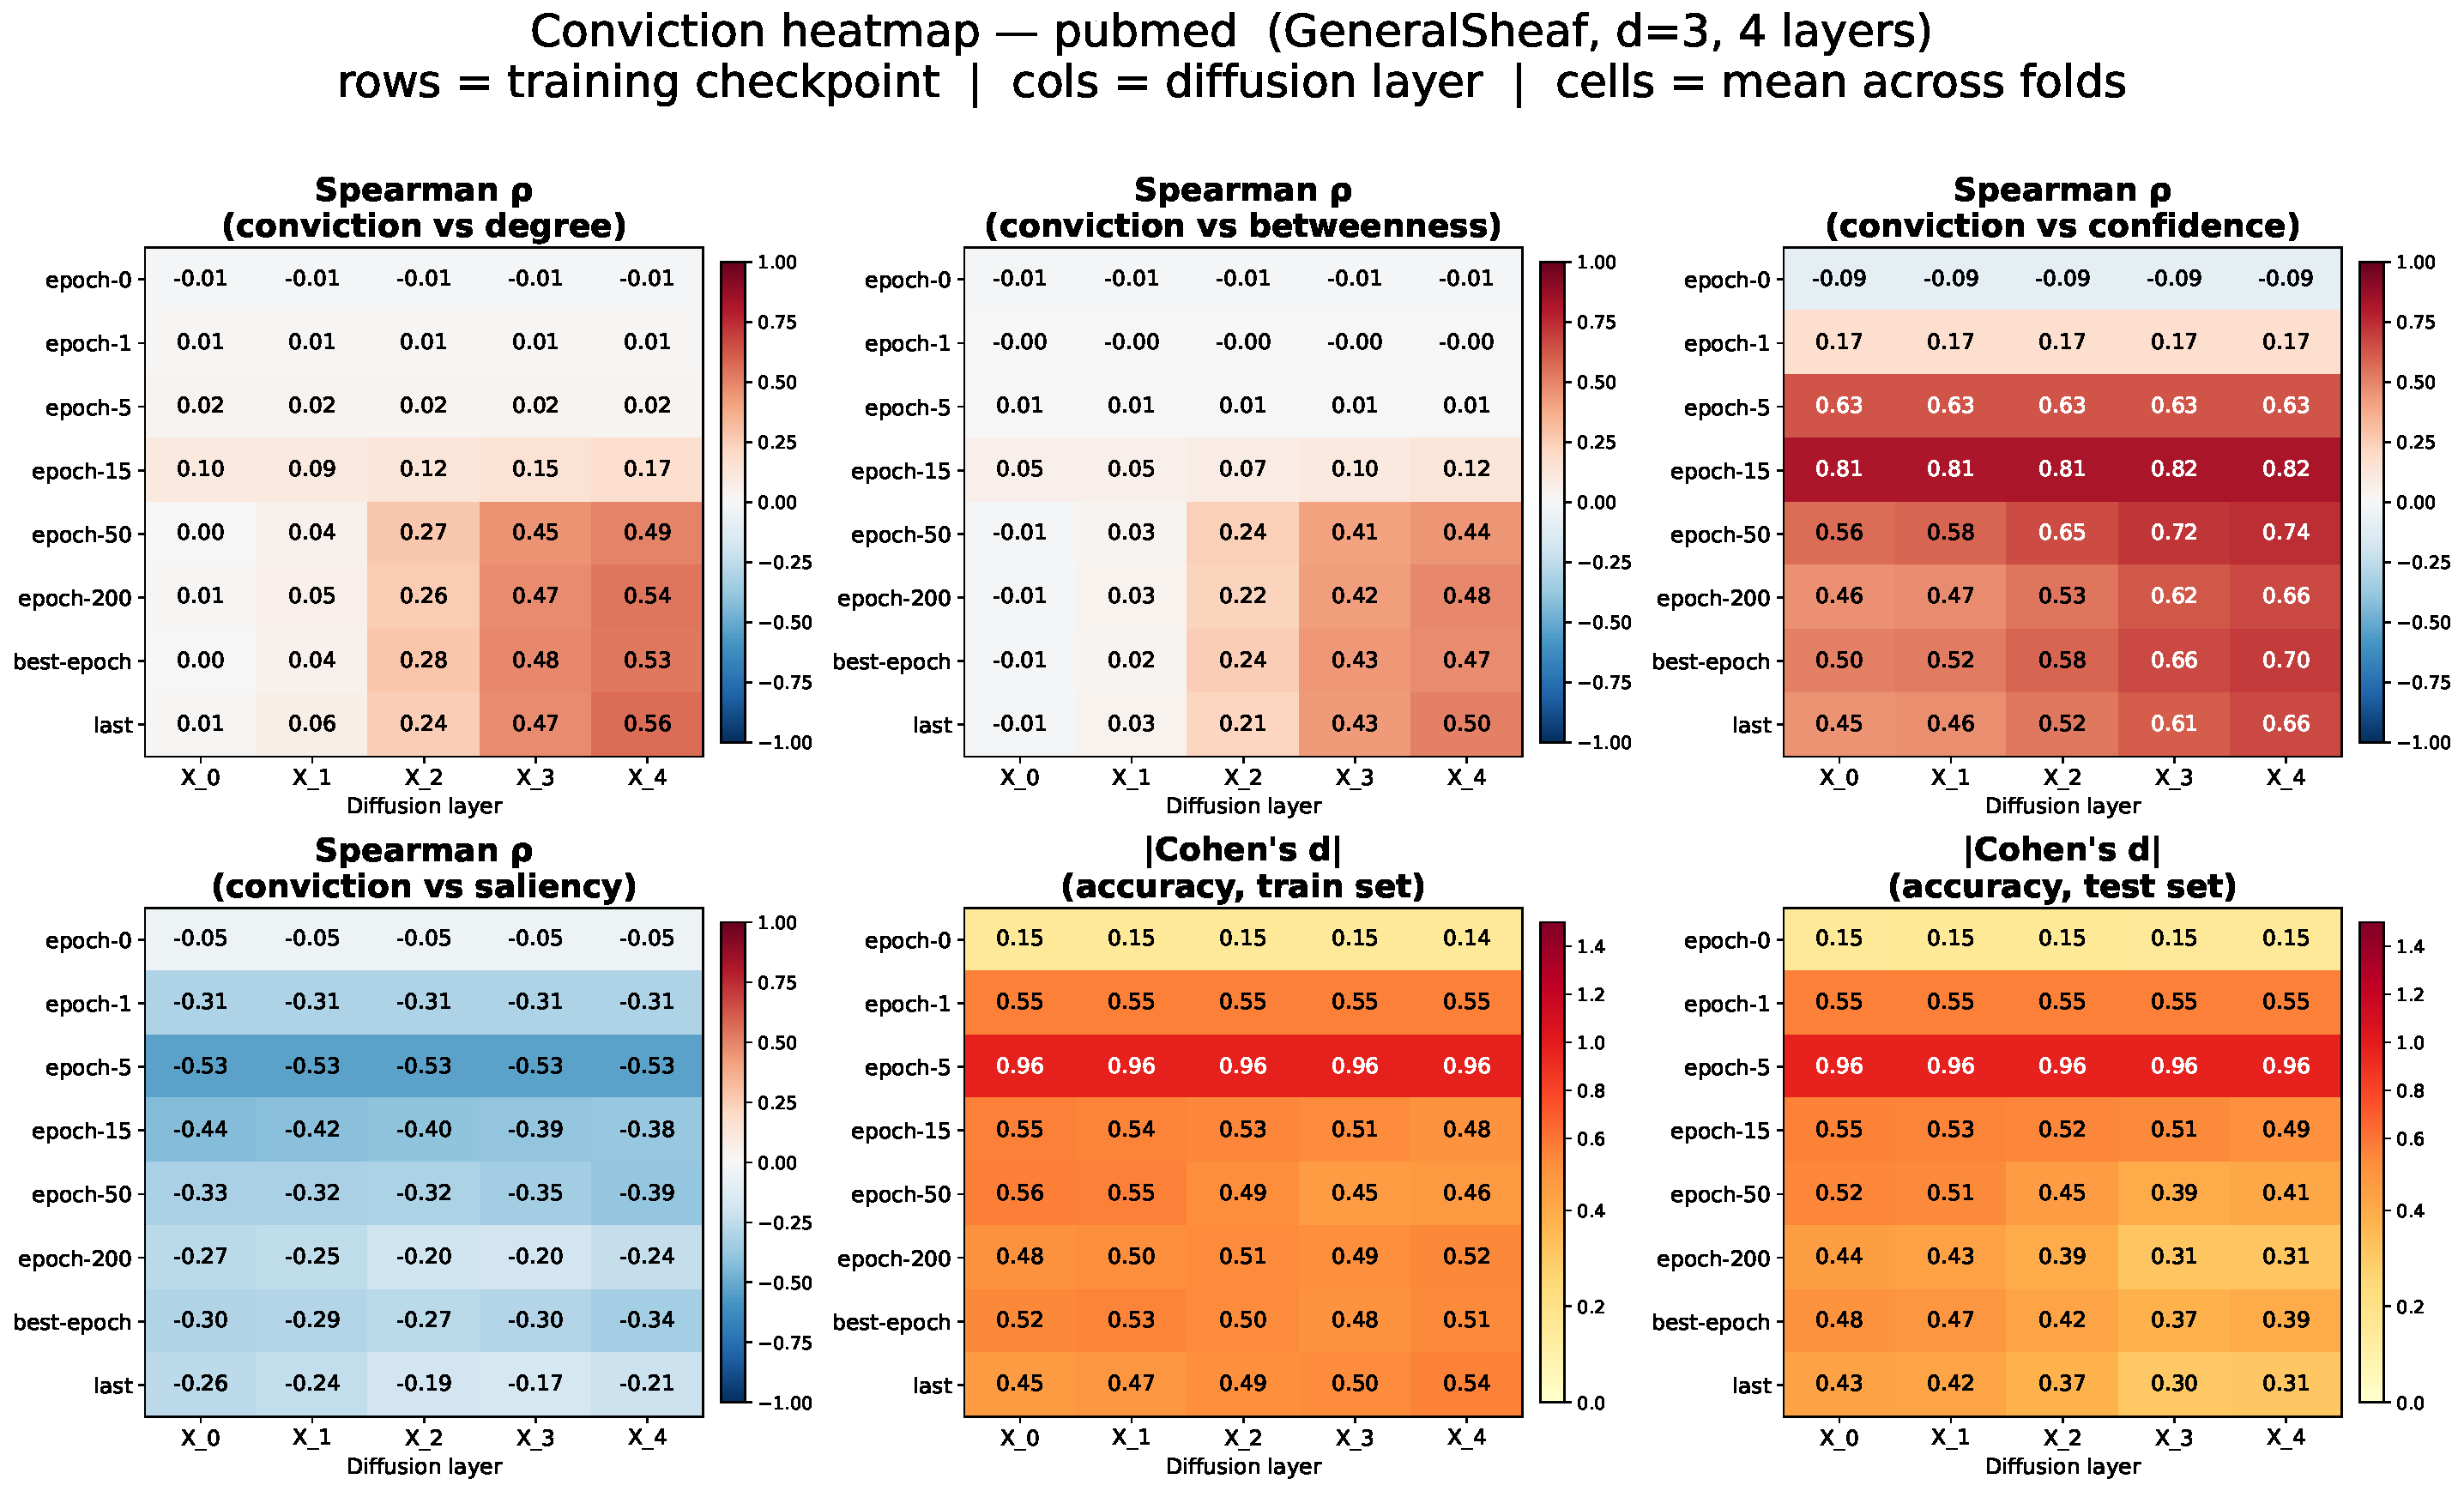
\includegraphics[width=\linewidth]{conviction_heatmap/GeneralSheaf/normalised_true/pubmed_GeneralSheaf_d3_4L_Norm_True_conviction_heatmap.pdf}
\end{figure}
\end{frame}

\begin{frame}{Questions --- GeneralSheaf, $d=5$, $L=4$, Norm=True}
\begin{figure}
    \centering
    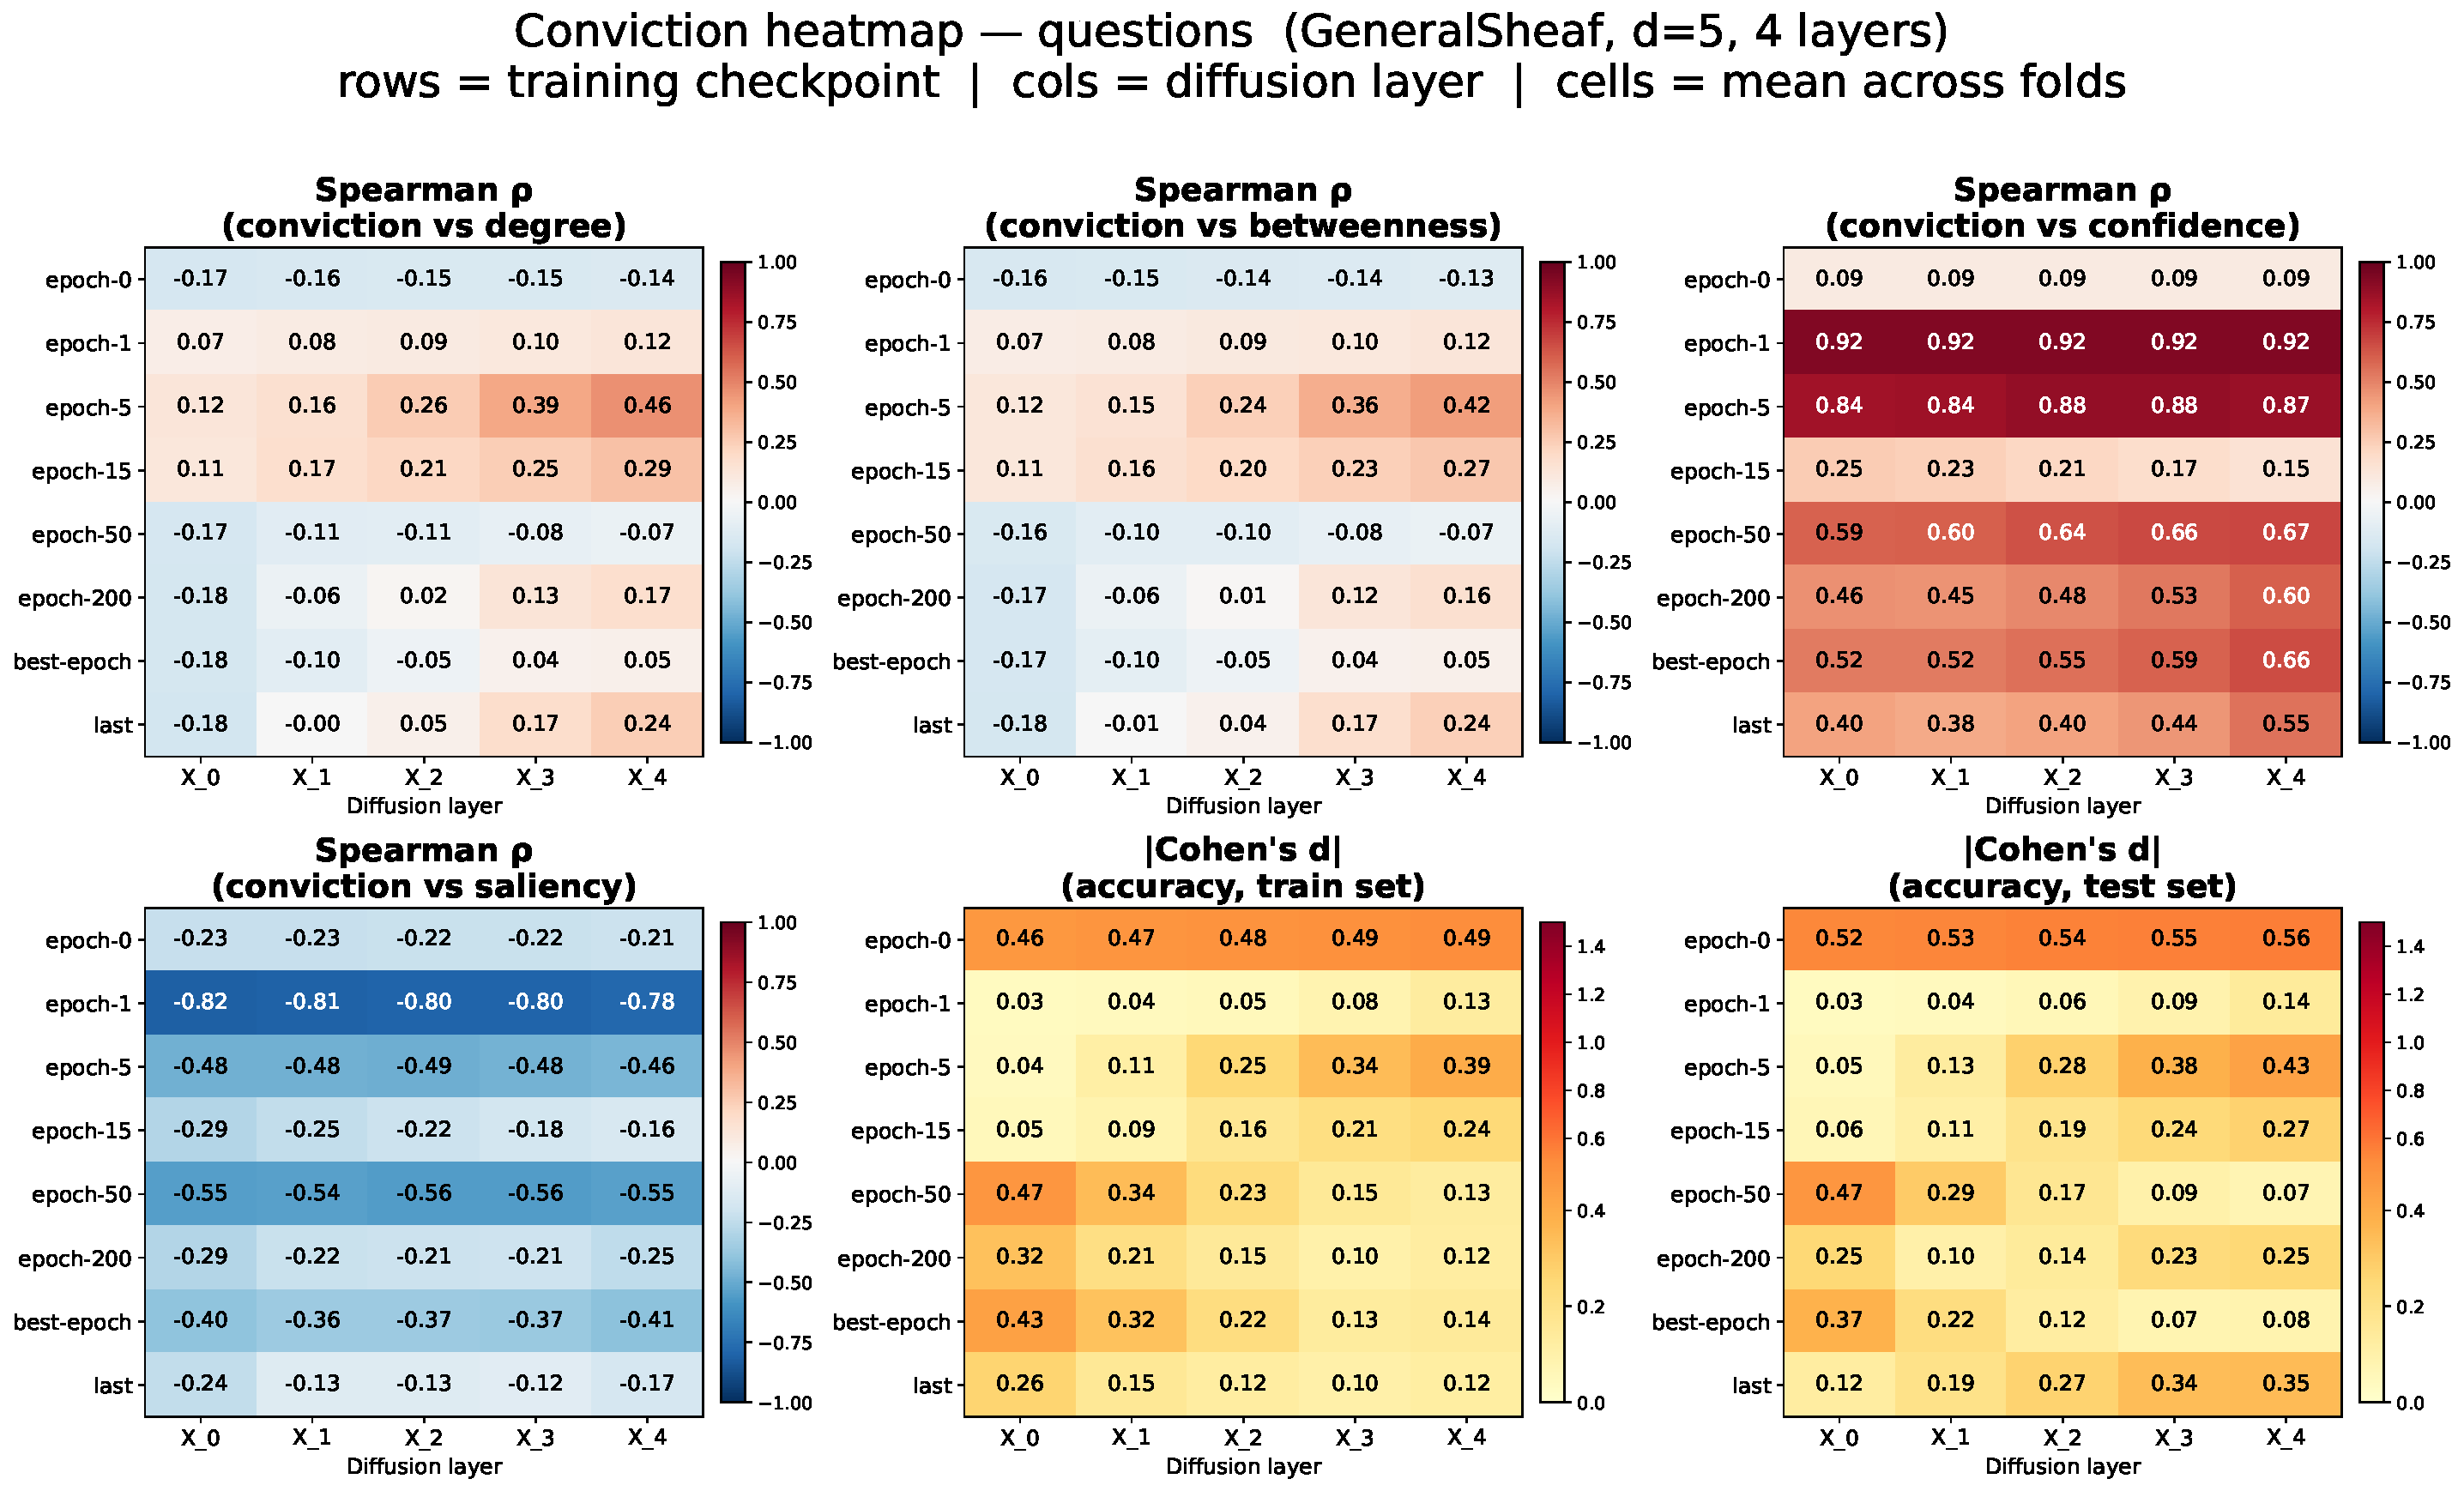
\includegraphics[width=\linewidth]{conviction_heatmap/GeneralSheaf/normalised_true/questions_GeneralSheaf_d5_4L_Norm_True_conviction_heatmap.pdf}
\end{figure}
\end{frame}

\begin{frame}{Roman Empire --- GeneralSheaf, $d=5$, $L=5$, Norm=True}
\begin{figure}
    \centering
    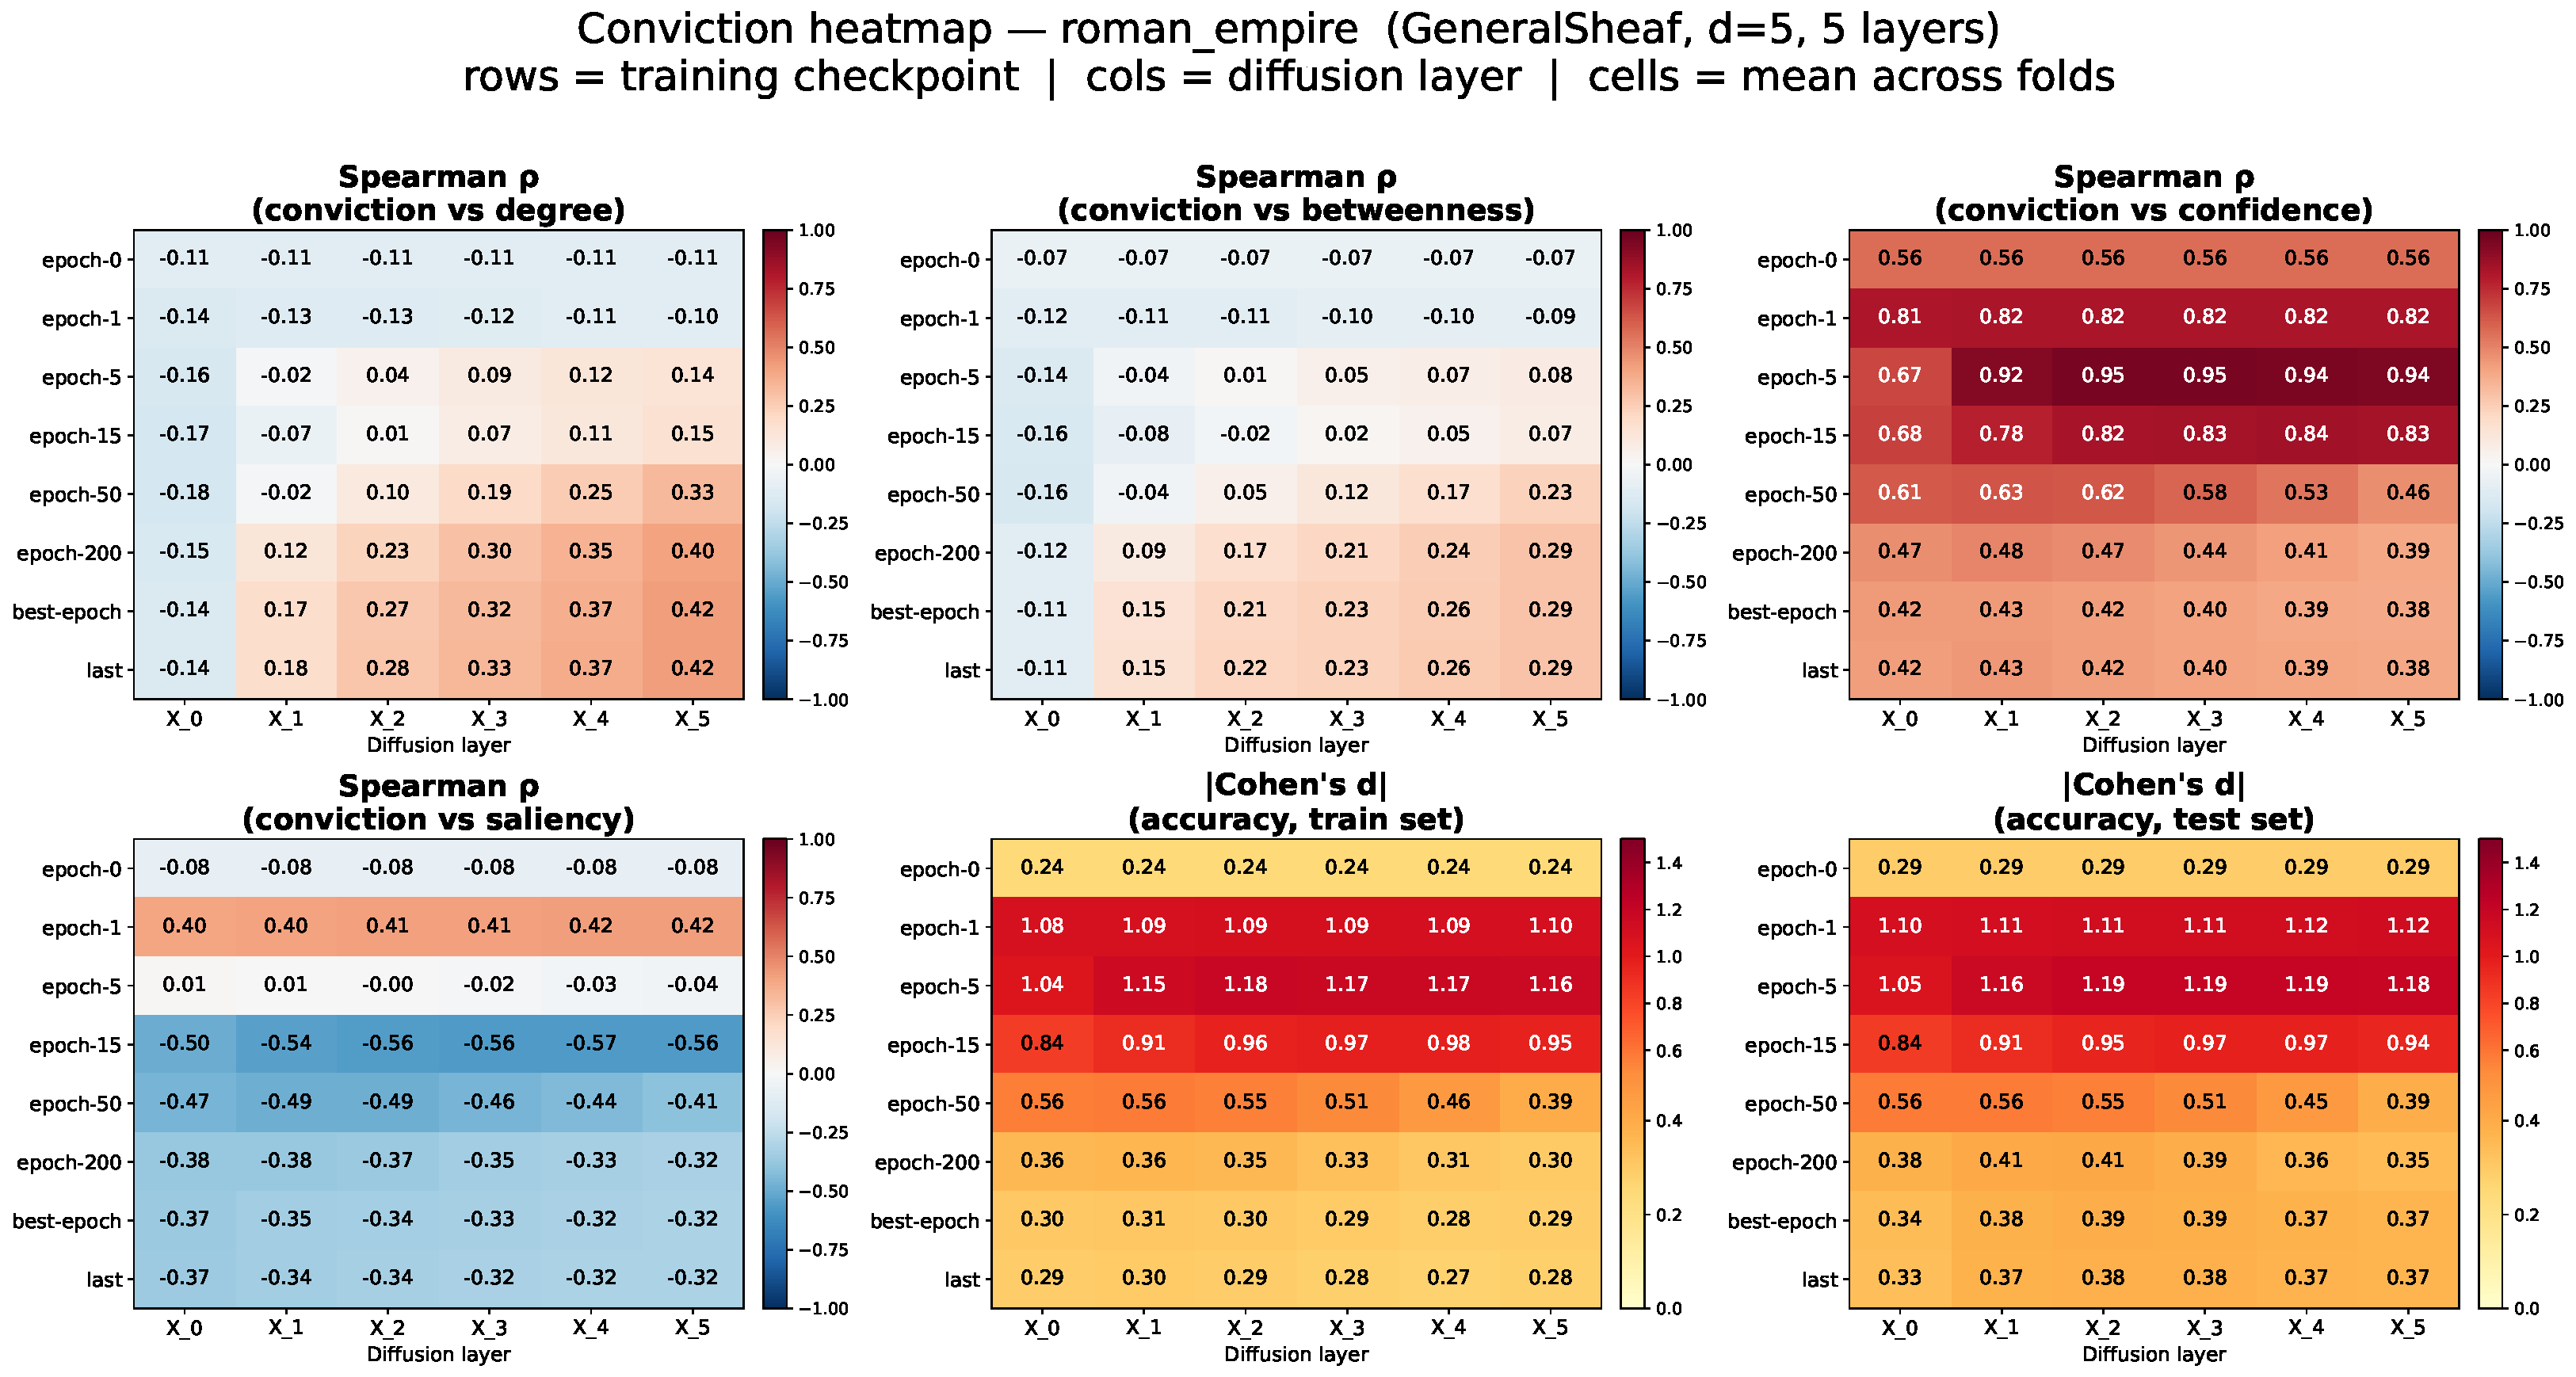
\includegraphics[width=\linewidth]{conviction_heatmap/GeneralSheaf/normalised_true/roman_empire_GeneralSheaf_d5_5L_Norm_True_conviction_heatmap.pdf}
\end{figure}
\end{frame}

\begin{frame}{Tolokers --- GeneralSheaf, $d=3$, $L=4$, Norm=True}
\begin{figure}
    \centering
    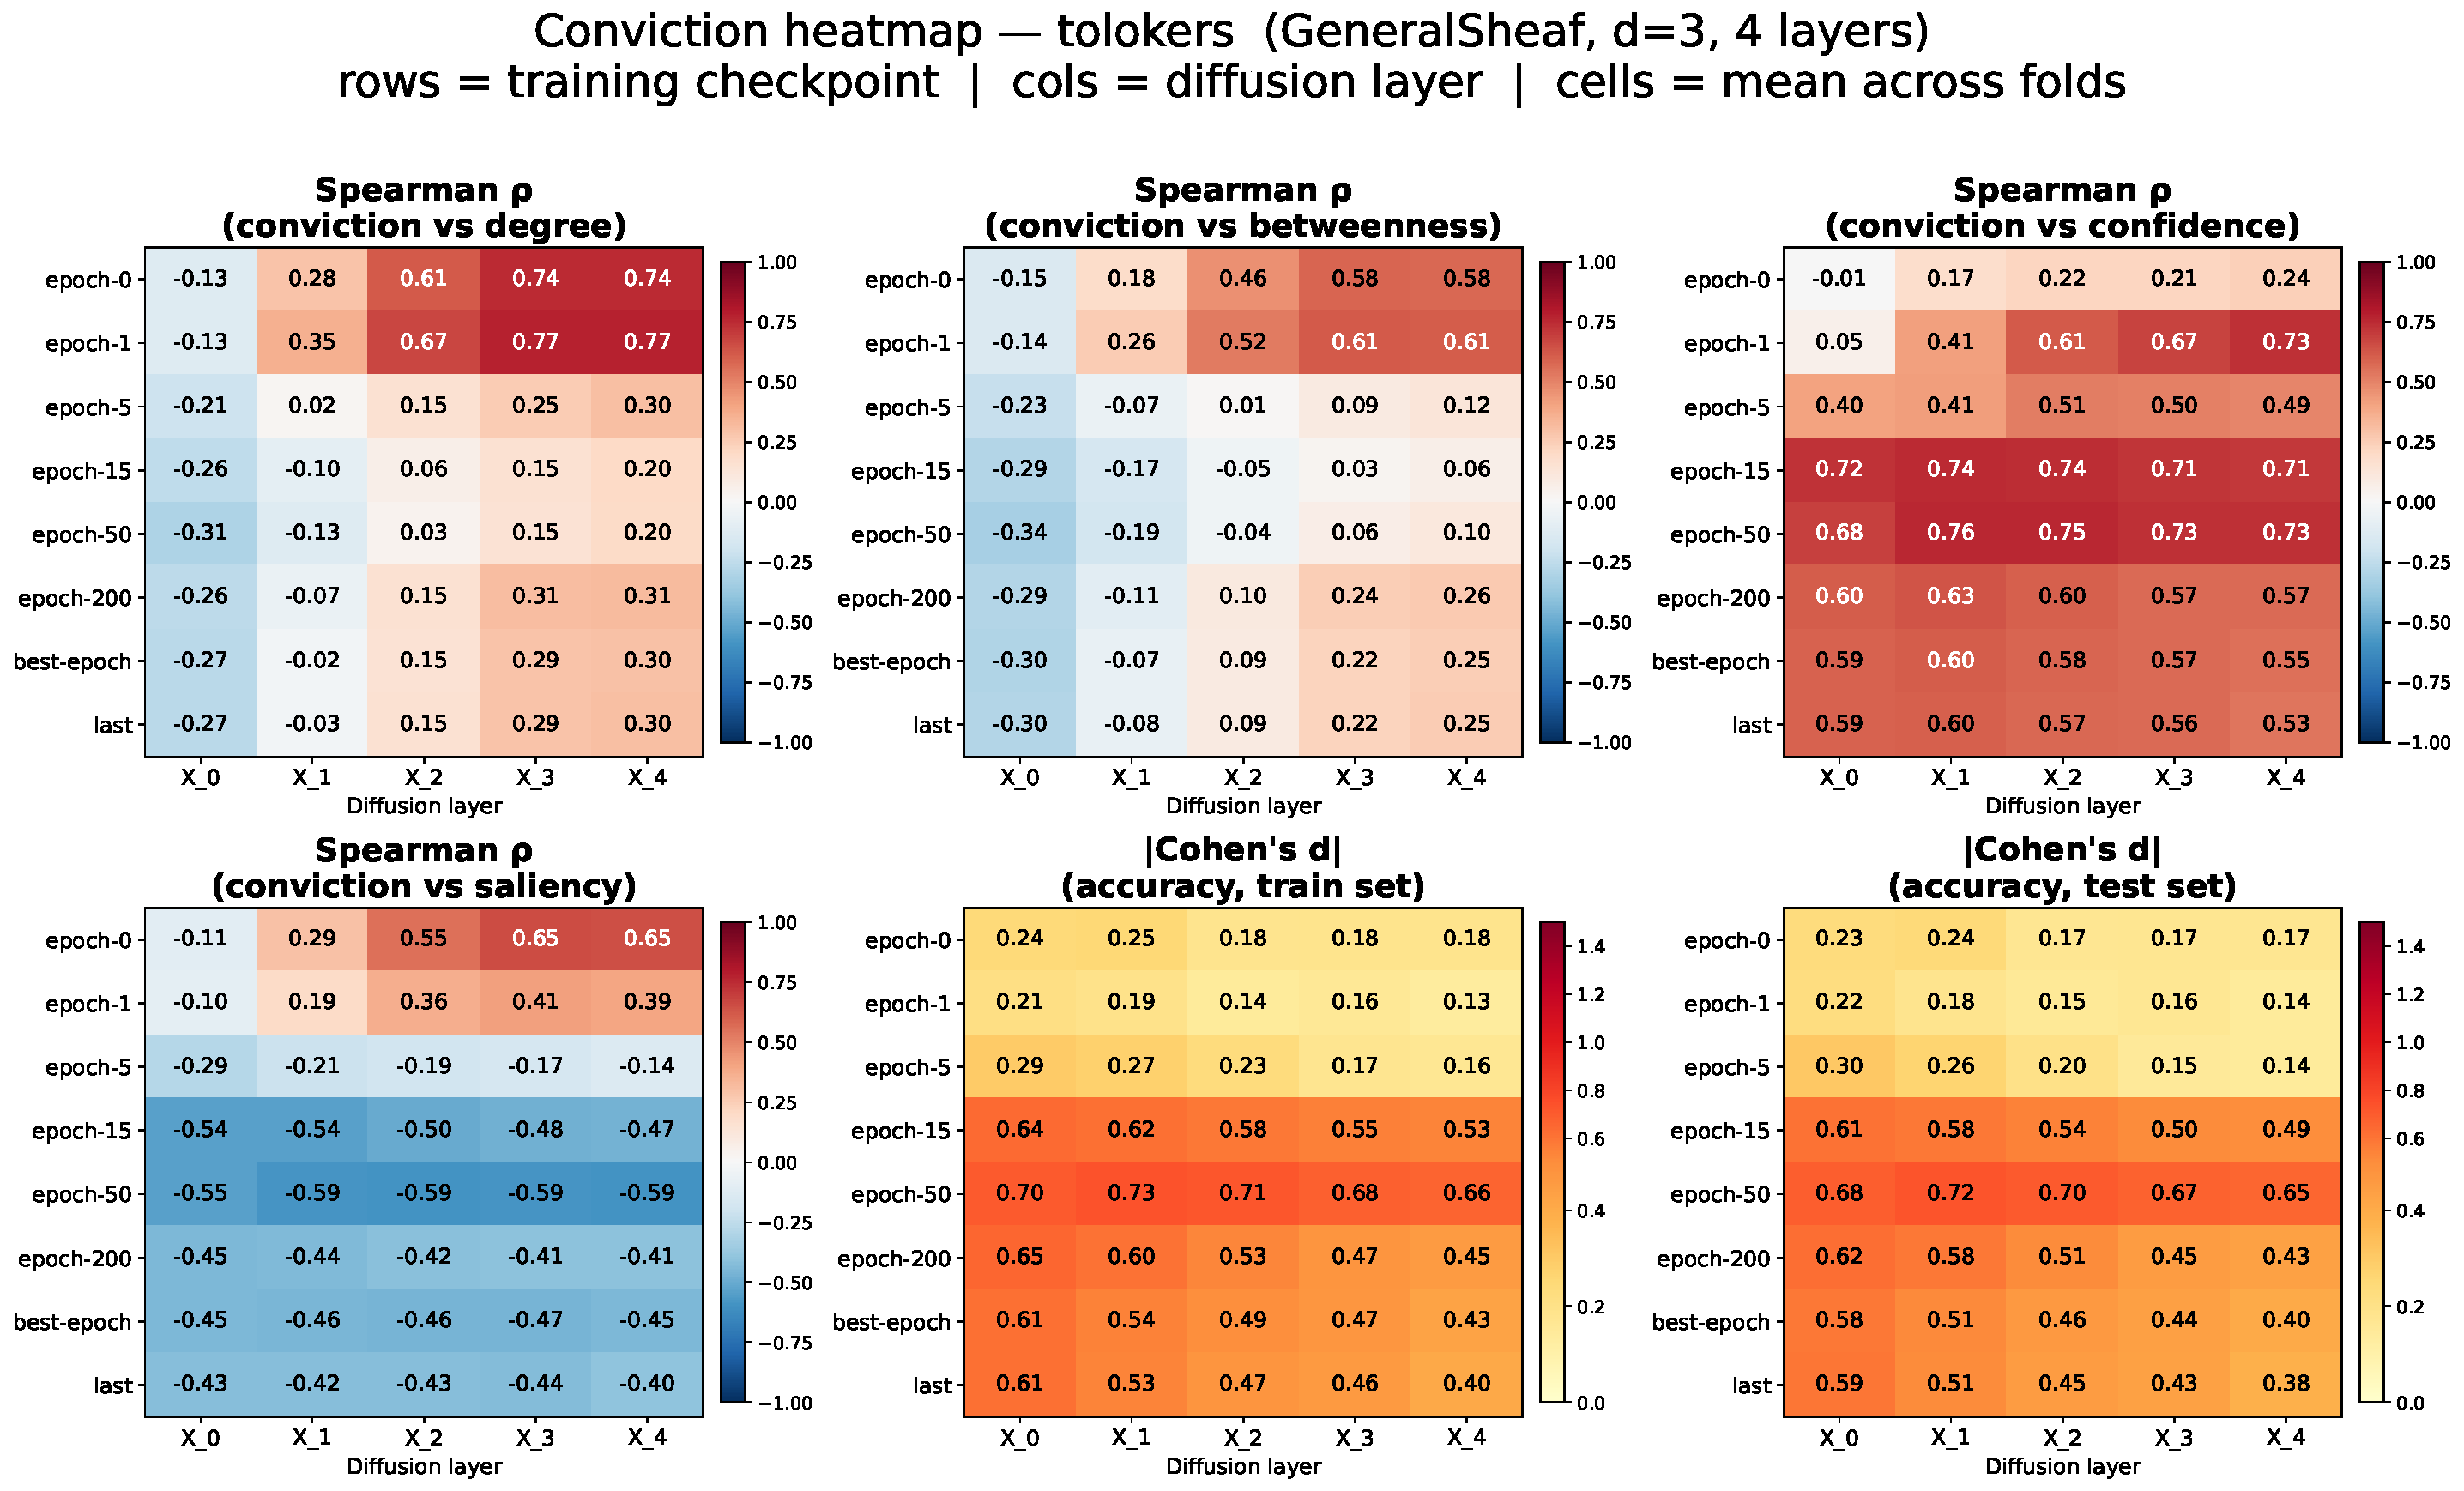
\includegraphics[width=\linewidth]{conviction_heatmap/GeneralSheaf/normalised_true/tolokers_GeneralSheaf_d3_4L_Norm_True_conviction_heatmap.pdf}
\end{figure}
\end{frame}

\begin{frame}{Wisconsin --- GeneralSheaf, $d=2$, $L=2$, Norm=True}
\begin{figure}
    \centering
    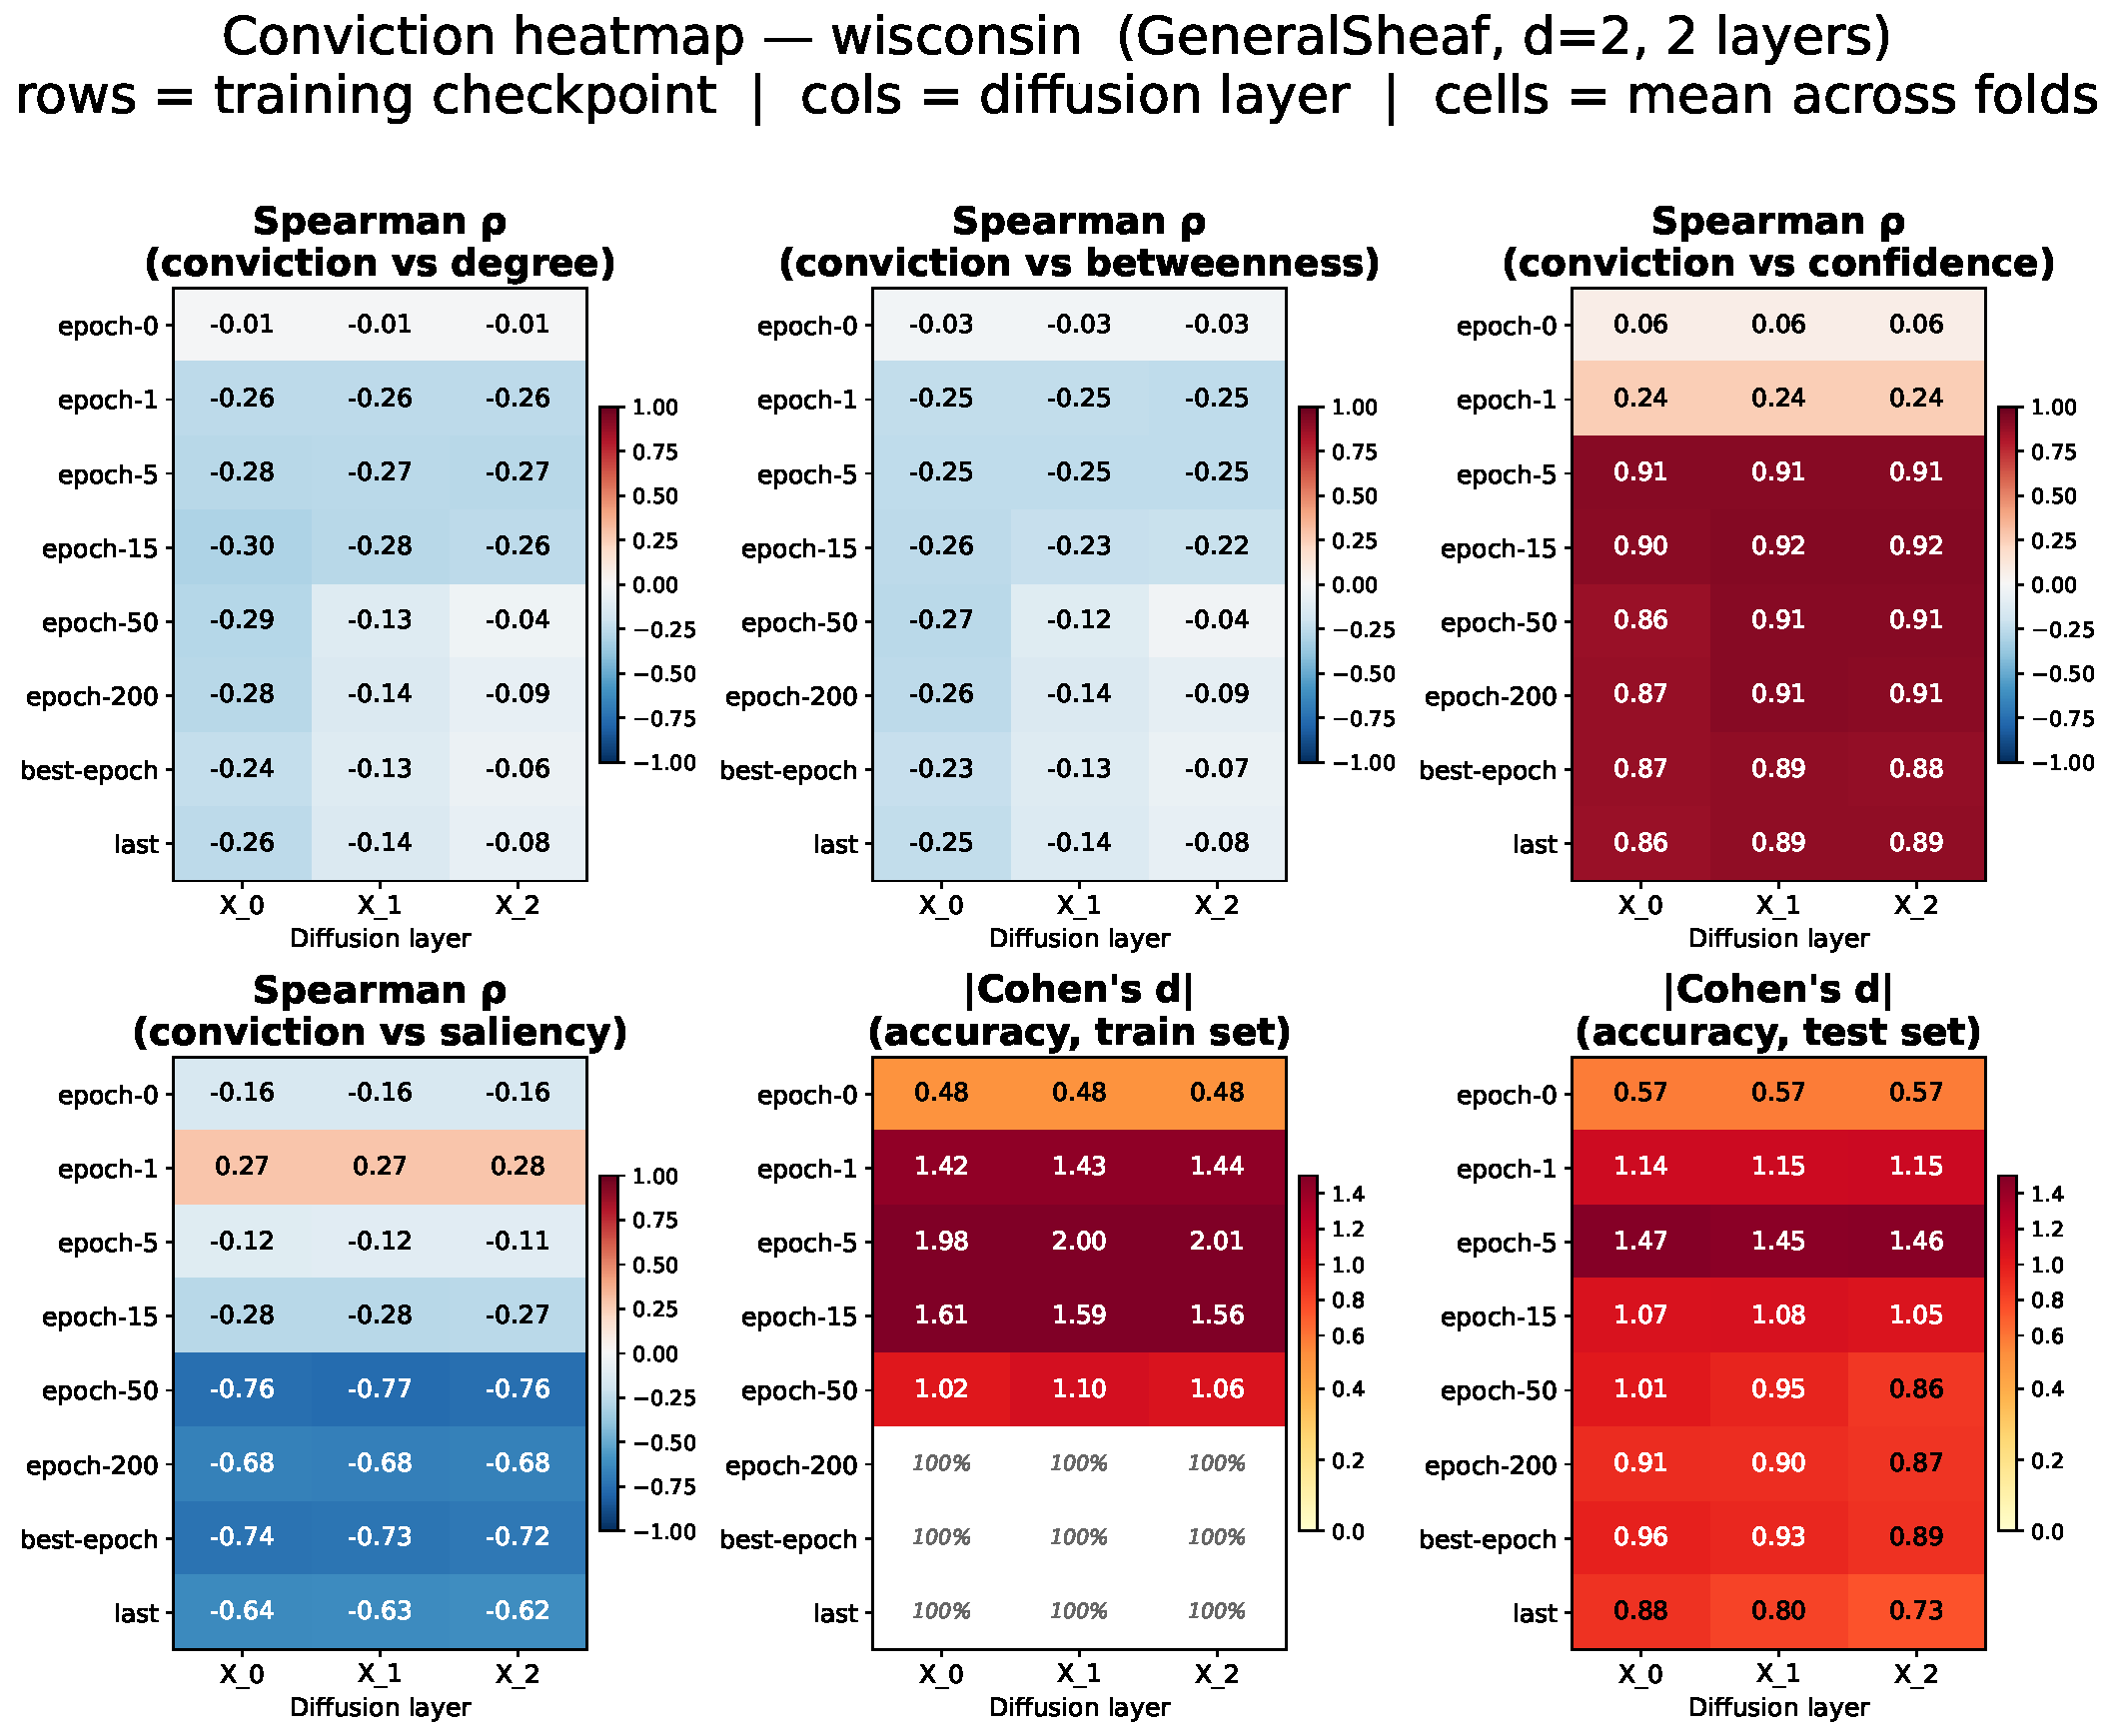
\includegraphics[width=0.8\linewidth]{conviction_heatmap/GeneralSheaf/normalised_true/wisconsin_GeneralSheaf_d2_2L_Norm_True_conviction_heatmap.pdf}
\end{figure}
\end{frame}




% ══════════════════════════════════════════════════════════════════════════════
%  SECTION 3 — Scatter, GeneralSheaf, normalised=True
% ══════════════════════════════════════════════════════════════════════════════

\begin{frame}{}
\centering
\Huge\textbf{Conviction Scatter}\\[6pt]
\Large GeneralSheaf \quad (\texttt{normalised=True})
\end{frame}

\begin{frame}{Amazon Ratings --- GeneralSheaf, $d=5$, $L=5$, Norm=True}
\begin{figure}
    \centering
    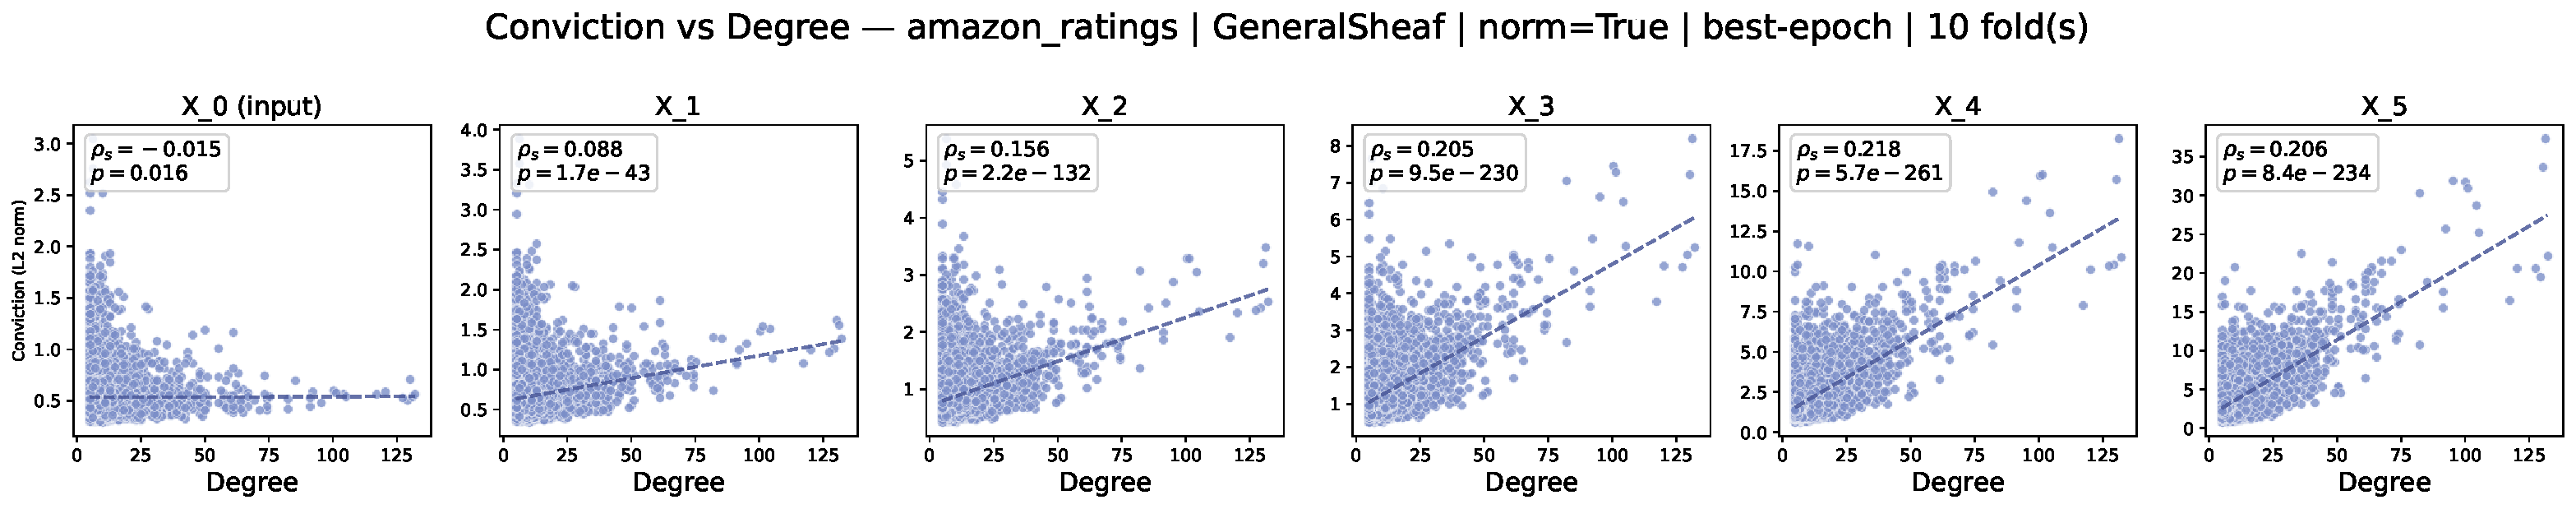
\includegraphics[width=\linewidth]{conviction_scatter/GeneralSheaf/normalised_true/amazon_ratings_GeneralSheaf_d5_5L_Norm_True_conviction_scatter.pdf}
\end{figure}
\end{frame}

\begin{frame}{Citeseer --- GeneralSheaf, $d=5$, $L=4$, Norm=True}
\begin{figure}
    \centering
    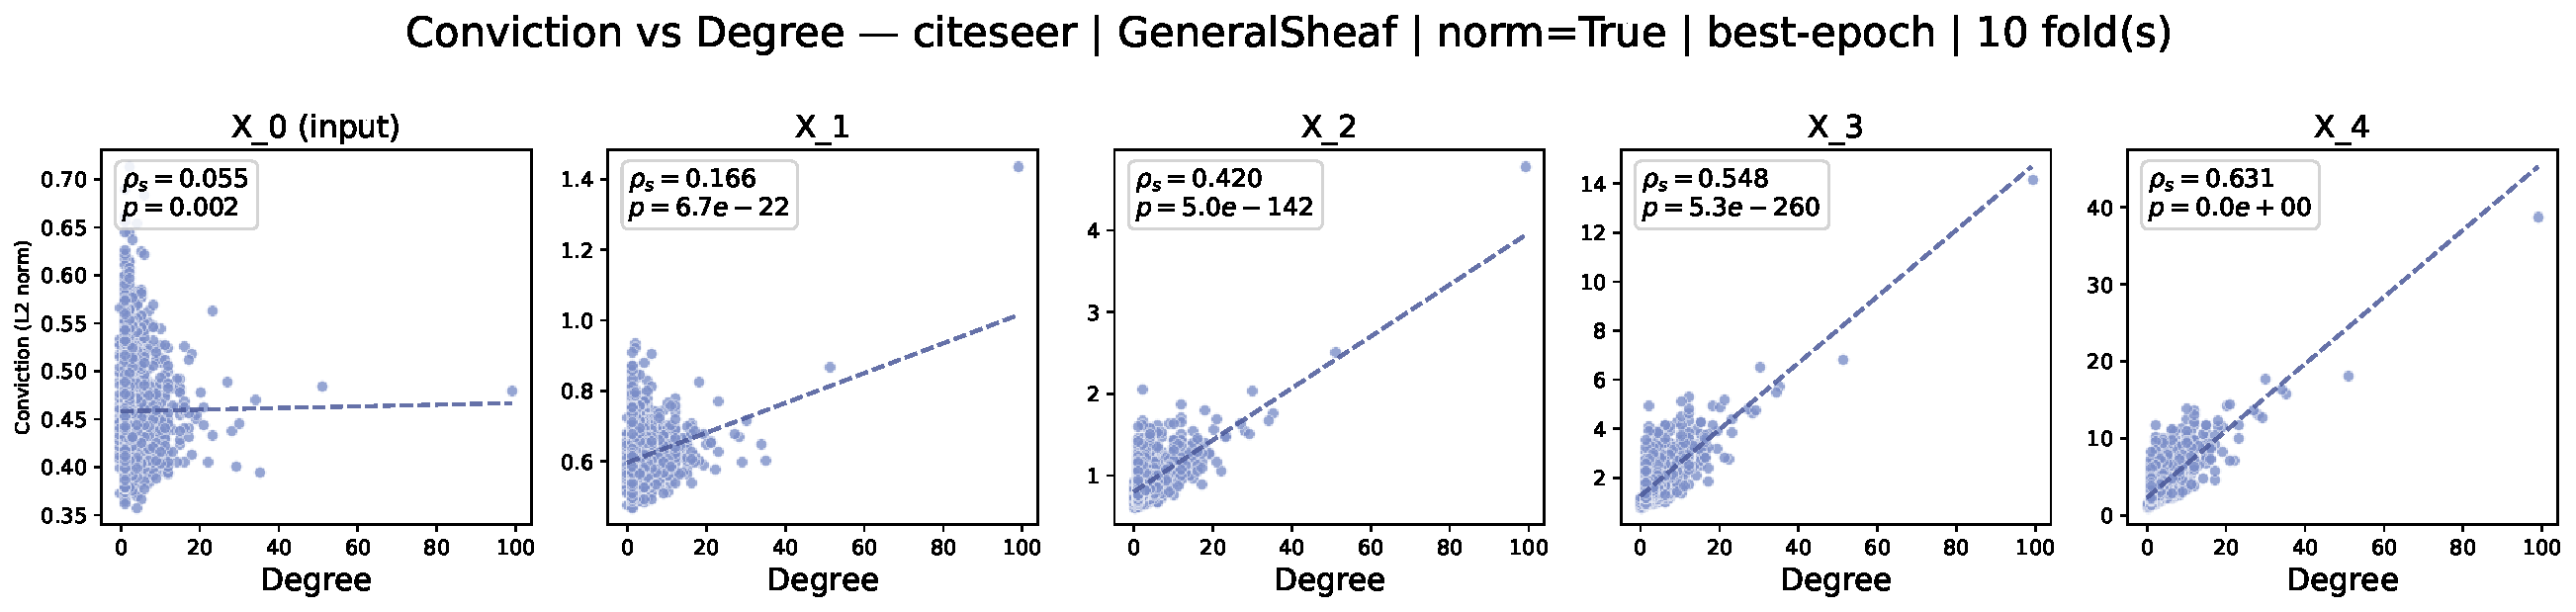
\includegraphics[width=\linewidth]{conviction_scatter/GeneralSheaf/normalised_true/citeseer_GeneralSheaf_d5_4L_Norm_True_conviction_scatter.pdf}
\end{figure}
\end{frame}

\begin{frame}{Cora --- GeneralSheaf, $d=5$, $L=3$, Norm=True}
\begin{figure}
    \centering
    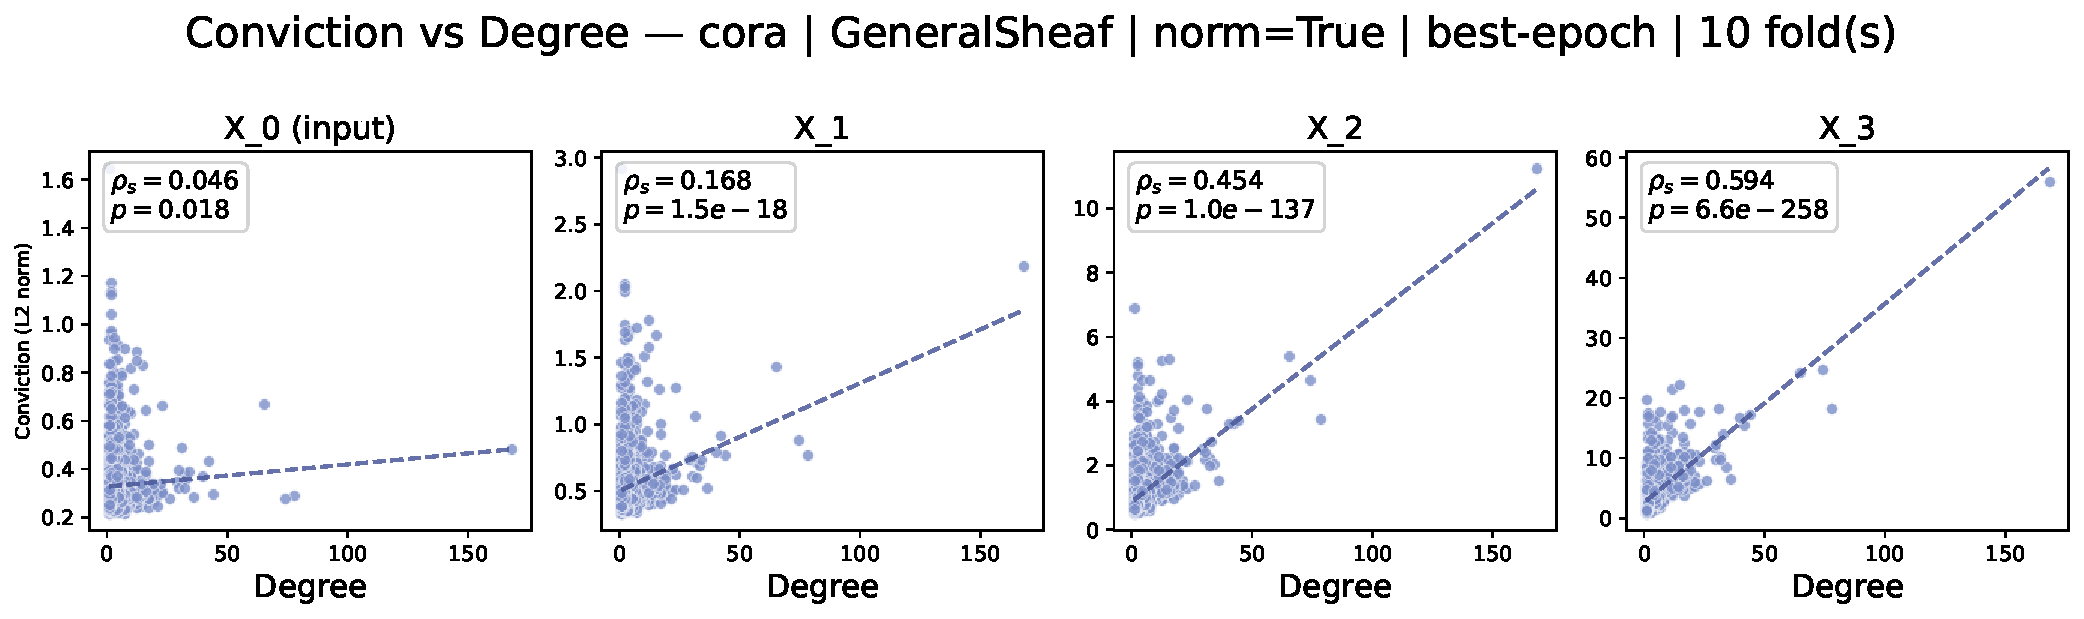
\includegraphics[width=\linewidth]{conviction_scatter/GeneralSheaf/normalised_true/cora_GeneralSheaf_d5_3L_Norm_True_conviction_scatter.pdf}
\end{figure}
\end{frame}

\begin{frame}{Cornell --- GeneralSheaf, $d=2$, $L=2$, Norm=True}
\begin{figure}
    \centering
    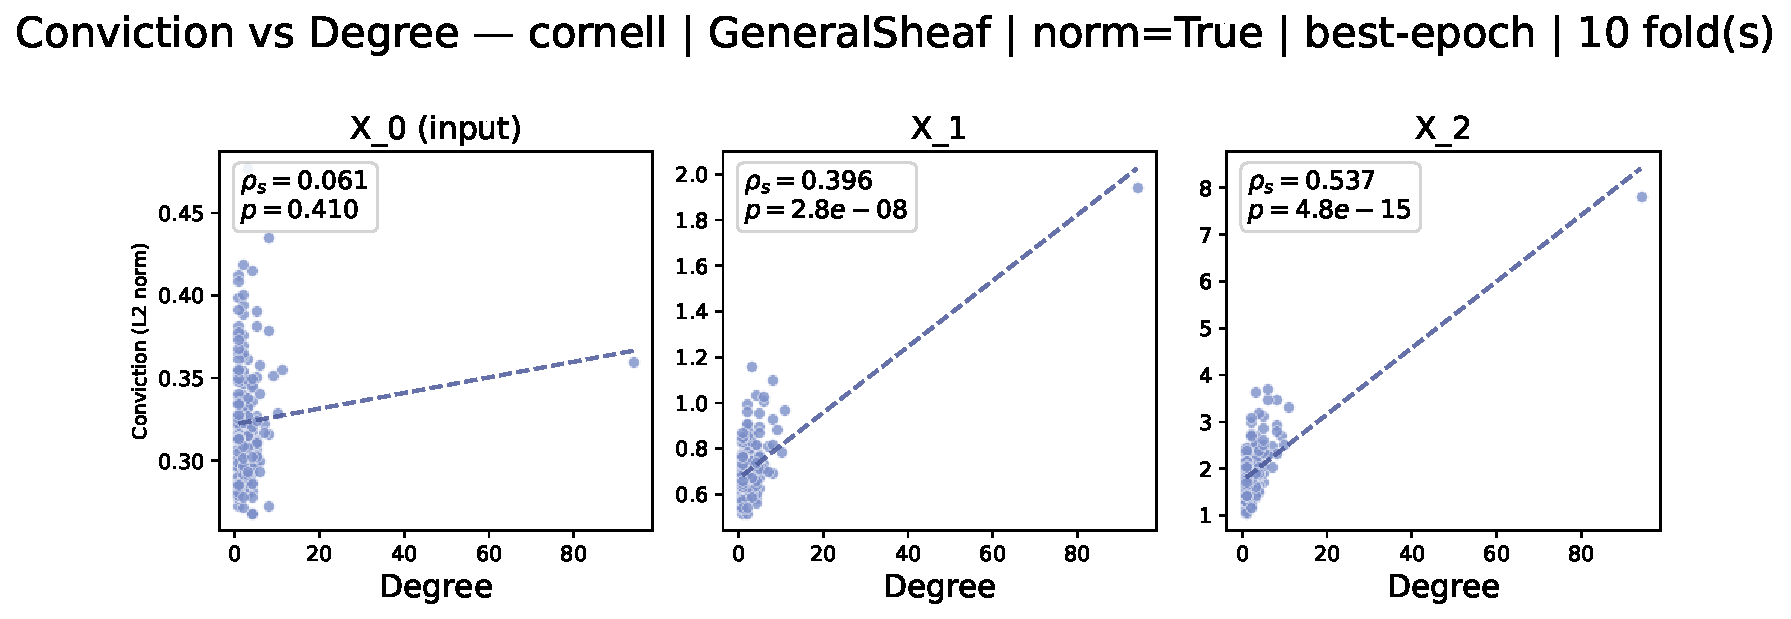
\includegraphics[width=0.8\linewidth]{conviction_scatter/GeneralSheaf/normalised_true/cornell_GeneralSheaf_d2_2L_Norm_True_conviction_scatter.pdf}
\end{figure}
\end{frame}

\begin{frame}{Minesweeper --- GeneralSheaf, $d=5$, $L=6$, Norm=True}
\begin{figure}
    \centering
    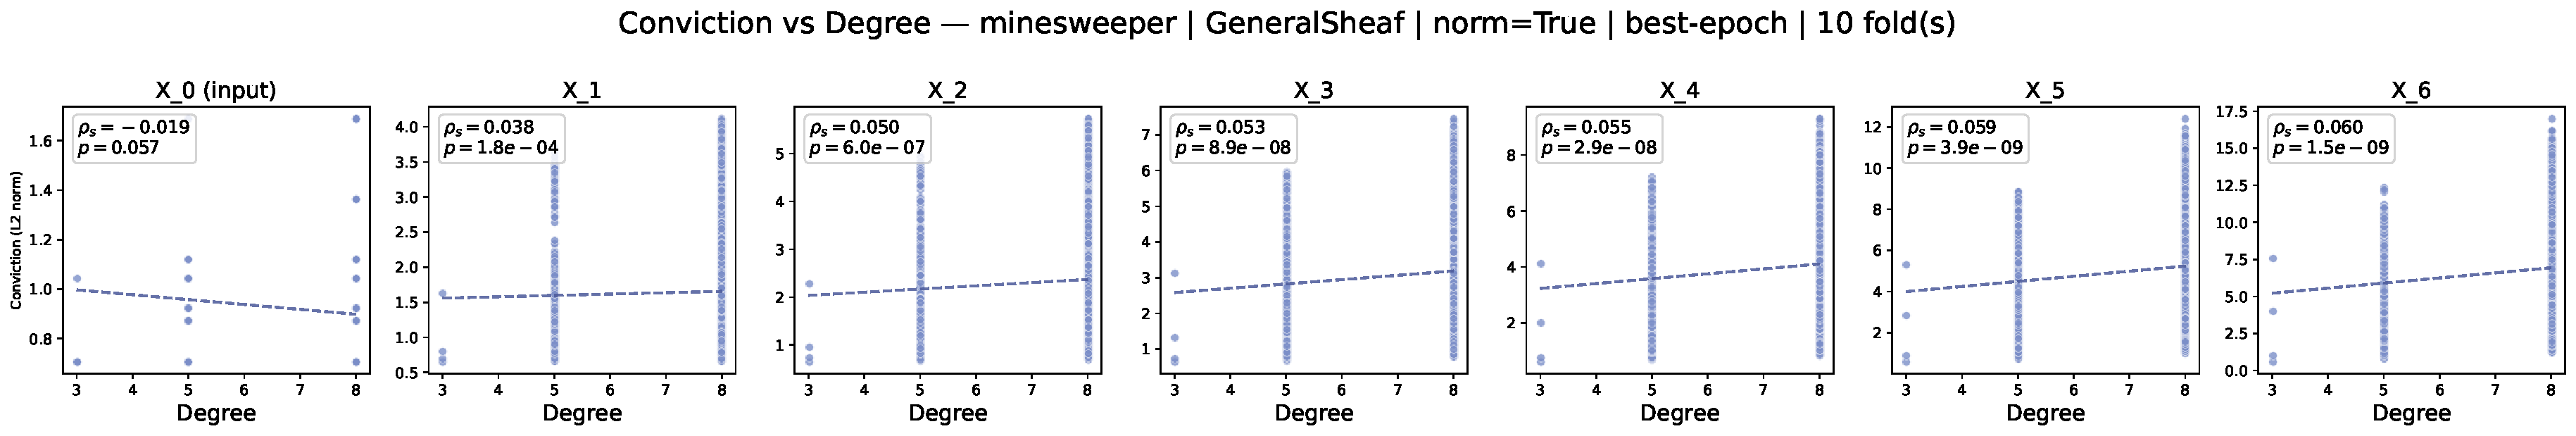
\includegraphics[width=\linewidth]{conviction_scatter/GeneralSheaf/normalised_true/minesweeper_GeneralSheaf_d5_6L_Norm_True_conviction_scatter.pdf}
\end{figure}
\end{frame}

\begin{frame}{Pubmed --- GeneralSheaf, $d=3$, $L=4$, Norm=True}
\begin{figure}
    \centering
    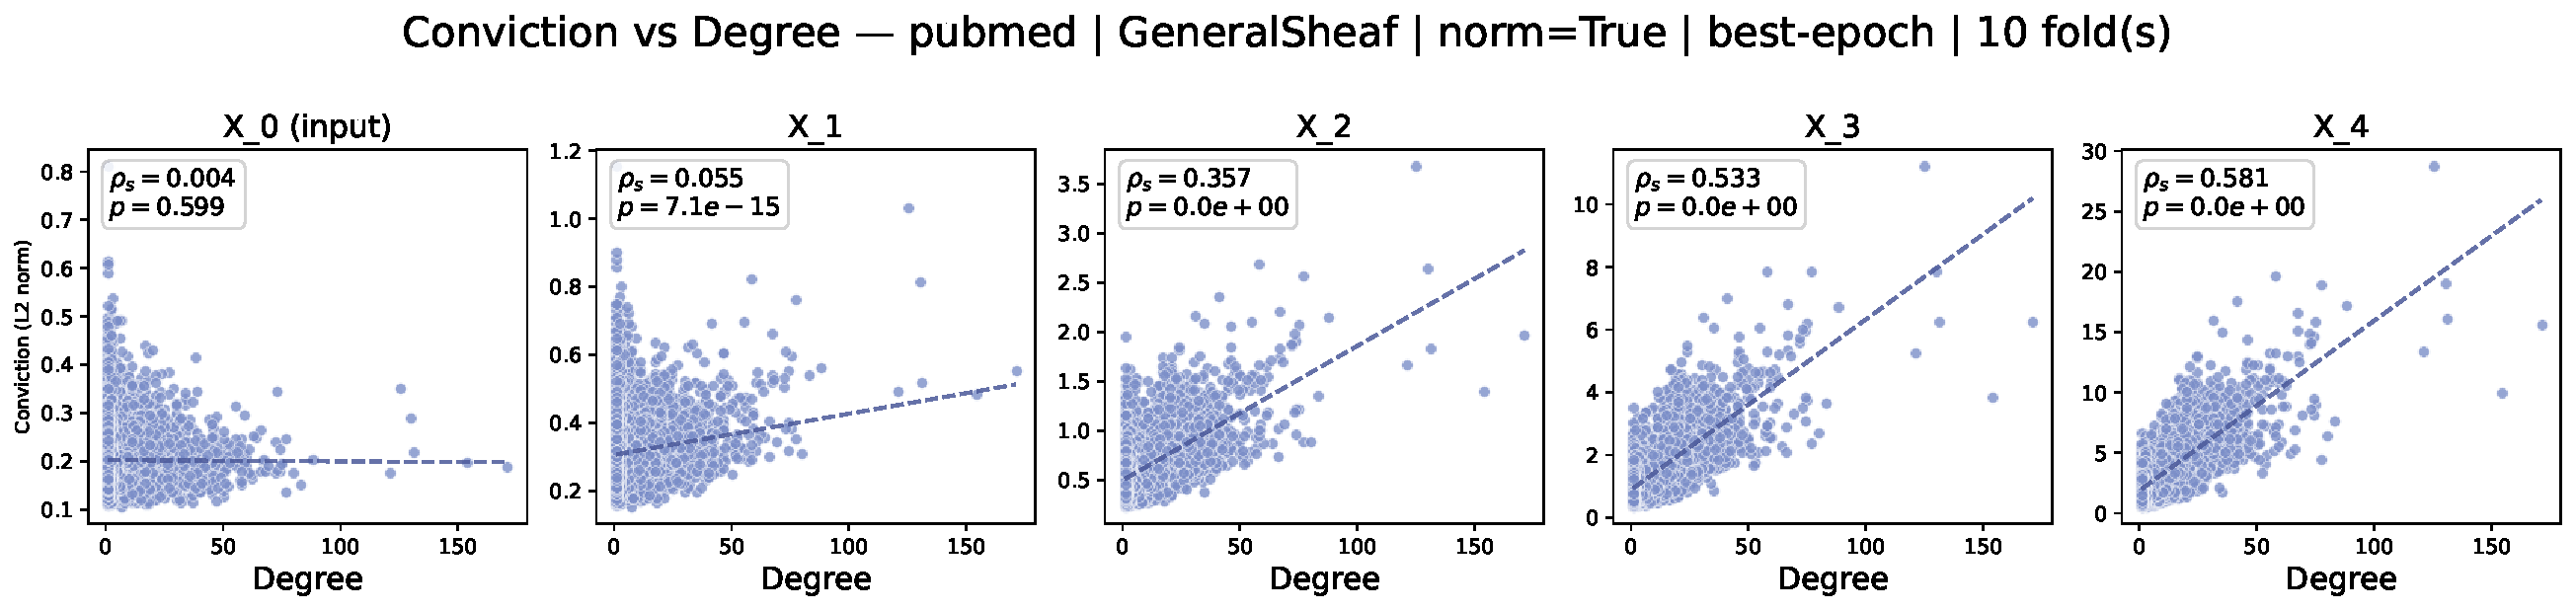
\includegraphics[width=\linewidth]{conviction_scatter/GeneralSheaf/normalised_true/pubmed_GeneralSheaf_d3_4L_Norm_True_conviction_scatter.pdf}
\end{figure}
\end{frame}

\begin{frame}{Questions --- GeneralSheaf, $d=5$, $L=4$, Norm=True}
\begin{figure}
    \centering
    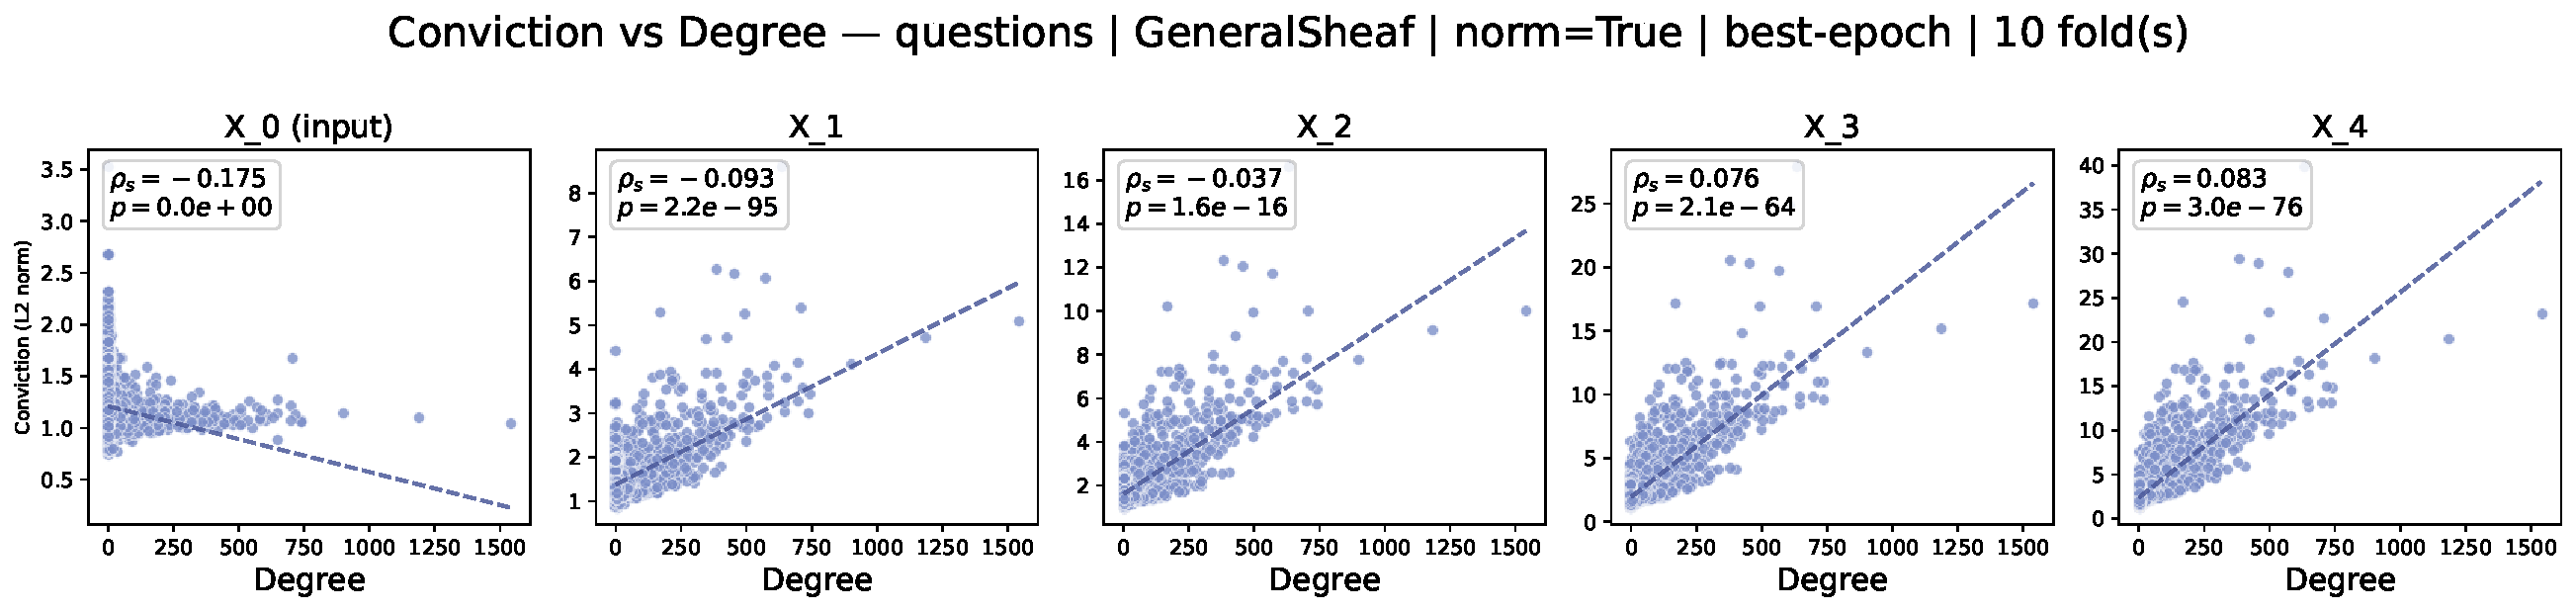
\includegraphics[width=\linewidth]{conviction_scatter/GeneralSheaf/normalised_true/questions_GeneralSheaf_d5_4L_Norm_True_conviction_scatter.pdf}
\end{figure}
\end{frame}

\begin{frame}{Roman Empire --- GeneralSheaf, $d=5$, $L=5$, Norm=True}
\begin{figure}
    \centering
    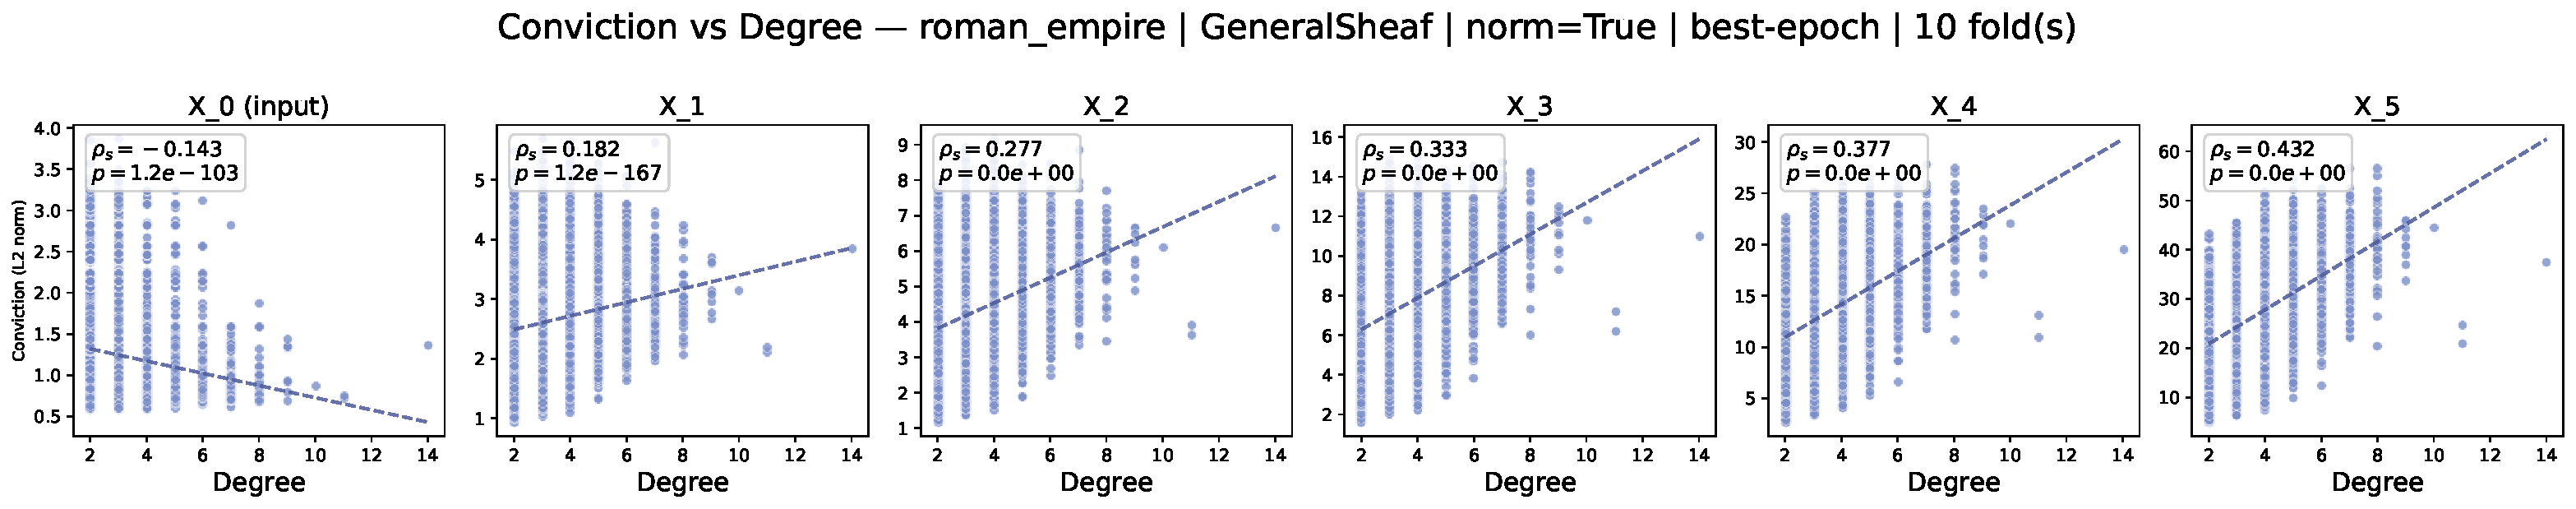
\includegraphics[width=\linewidth]{conviction_scatter/GeneralSheaf/normalised_true/roman_empire_GeneralSheaf_d5_5L_Norm_True_conviction_scatter.pdf}
\end{figure}
\end{frame}

\begin{frame}{Tolokers --- GeneralSheaf, $d=3$, $L=4$, Norm=True}
\begin{figure}
    \centering
    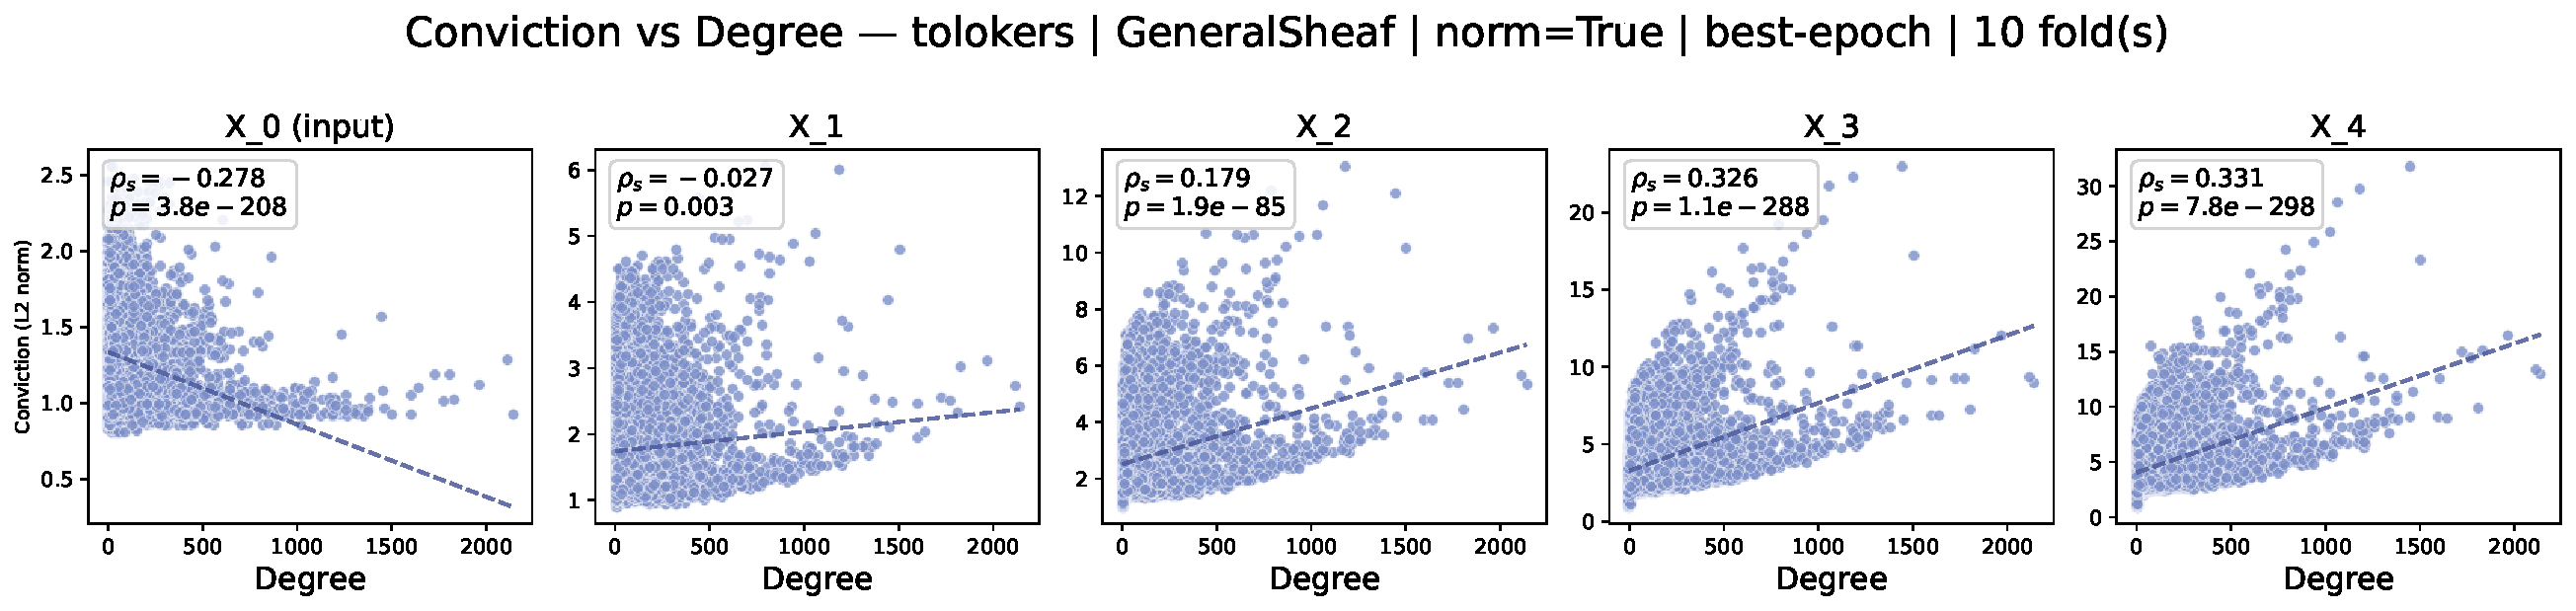
\includegraphics[width=\linewidth]{conviction_scatter/GeneralSheaf/normalised_true/tolokers_GeneralSheaf_d3_4L_Norm_True_conviction_scatter.pdf}
\end{figure}
\end{frame}

\begin{frame}{Wisconsin --- GeneralSheaf, $d=2$, $L=2$, Norm=True}
\begin{figure}
    \centering
    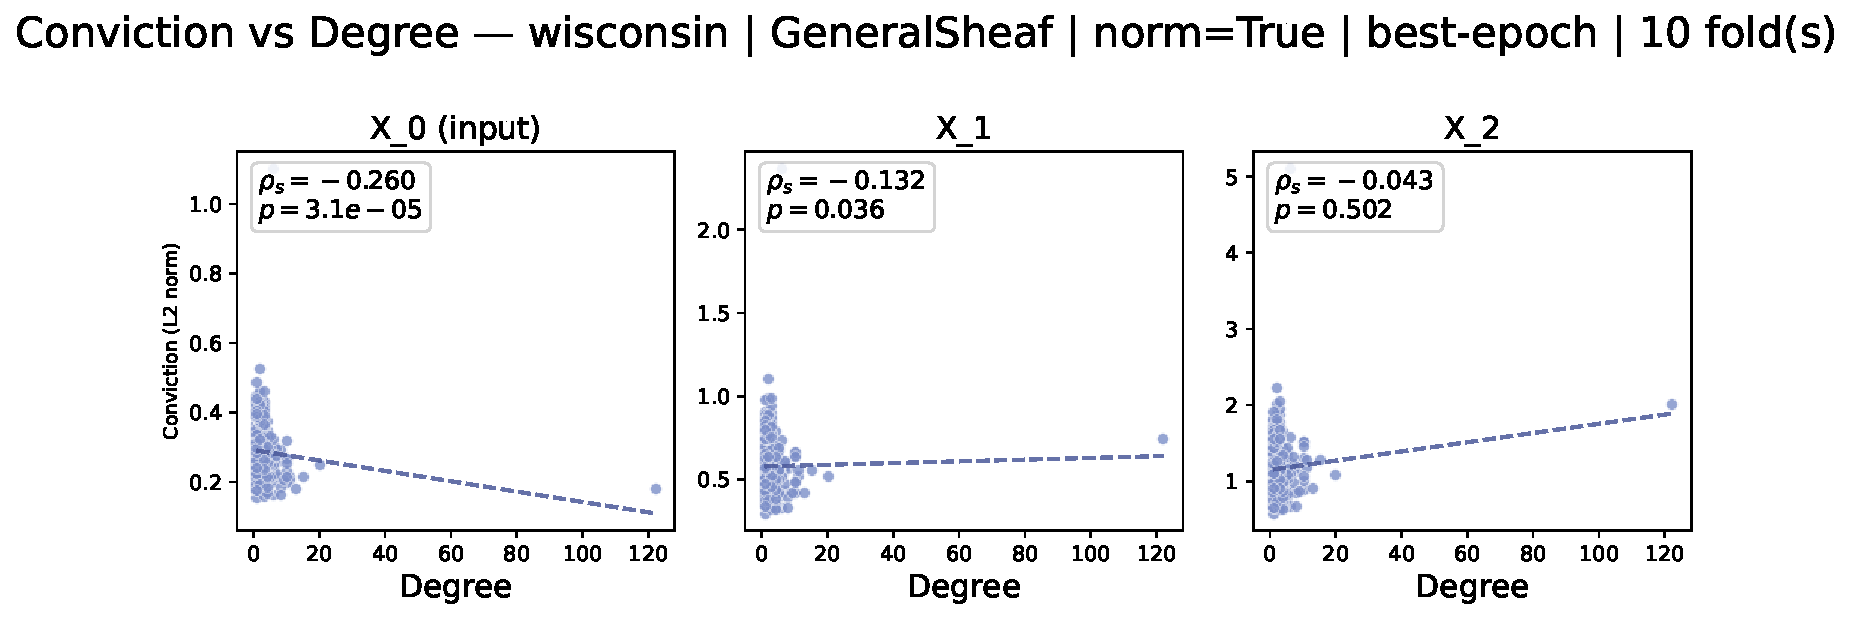
\includegraphics[width=0.8\linewidth]{conviction_scatter/GeneralSheaf/normalised_true/wisconsin_GeneralSheaf_d2_2L_Norm_True_conviction_scatter.pdf}
\end{figure}
\end{frame}




% ══════════════════════════════════════════════════════════════════════════════
%  SECTION 4 — Masking, BundleSheaf, normalised=False
% ══════════════════════════════════════════════════════════════════════════════

\begin{frame}{}
\centering
\Huge\textbf{Conviction Masking}\\[6pt]
\Large BundleSheaf \quad (\texttt{normalised=False})
\end{frame}

\begin{frame}{Amazon Ratings --- BundleSheaf, $d=5$, $L=5$, Norm=False}
\begin{figure}
    \centering
    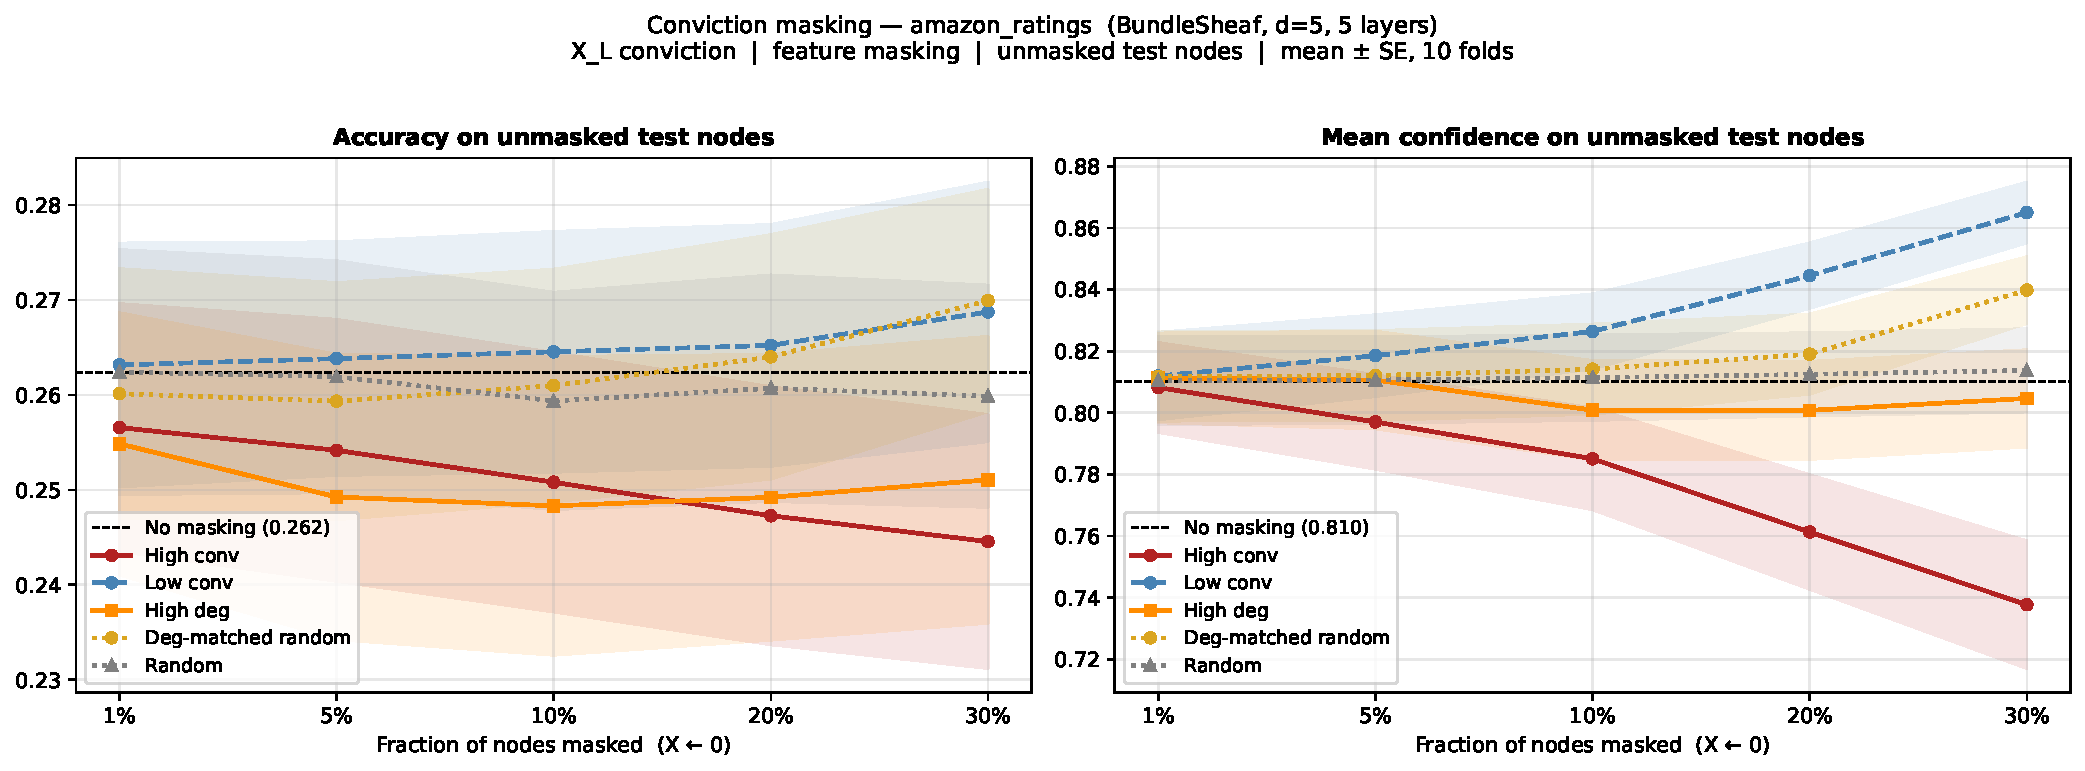
\includegraphics[width=\linewidth]{accuracy_ranking/BundleSheaf/normalised_false/amazon_ratings_BundleSheaf_d5_5L_Norm_False_conviction_masking.pdf}
\end{figure}
\end{frame}

\begin{frame}{Citeseer --- BundleSheaf, $d=5$, $L=4$, Norm=False}
\begin{figure}
    \centering
    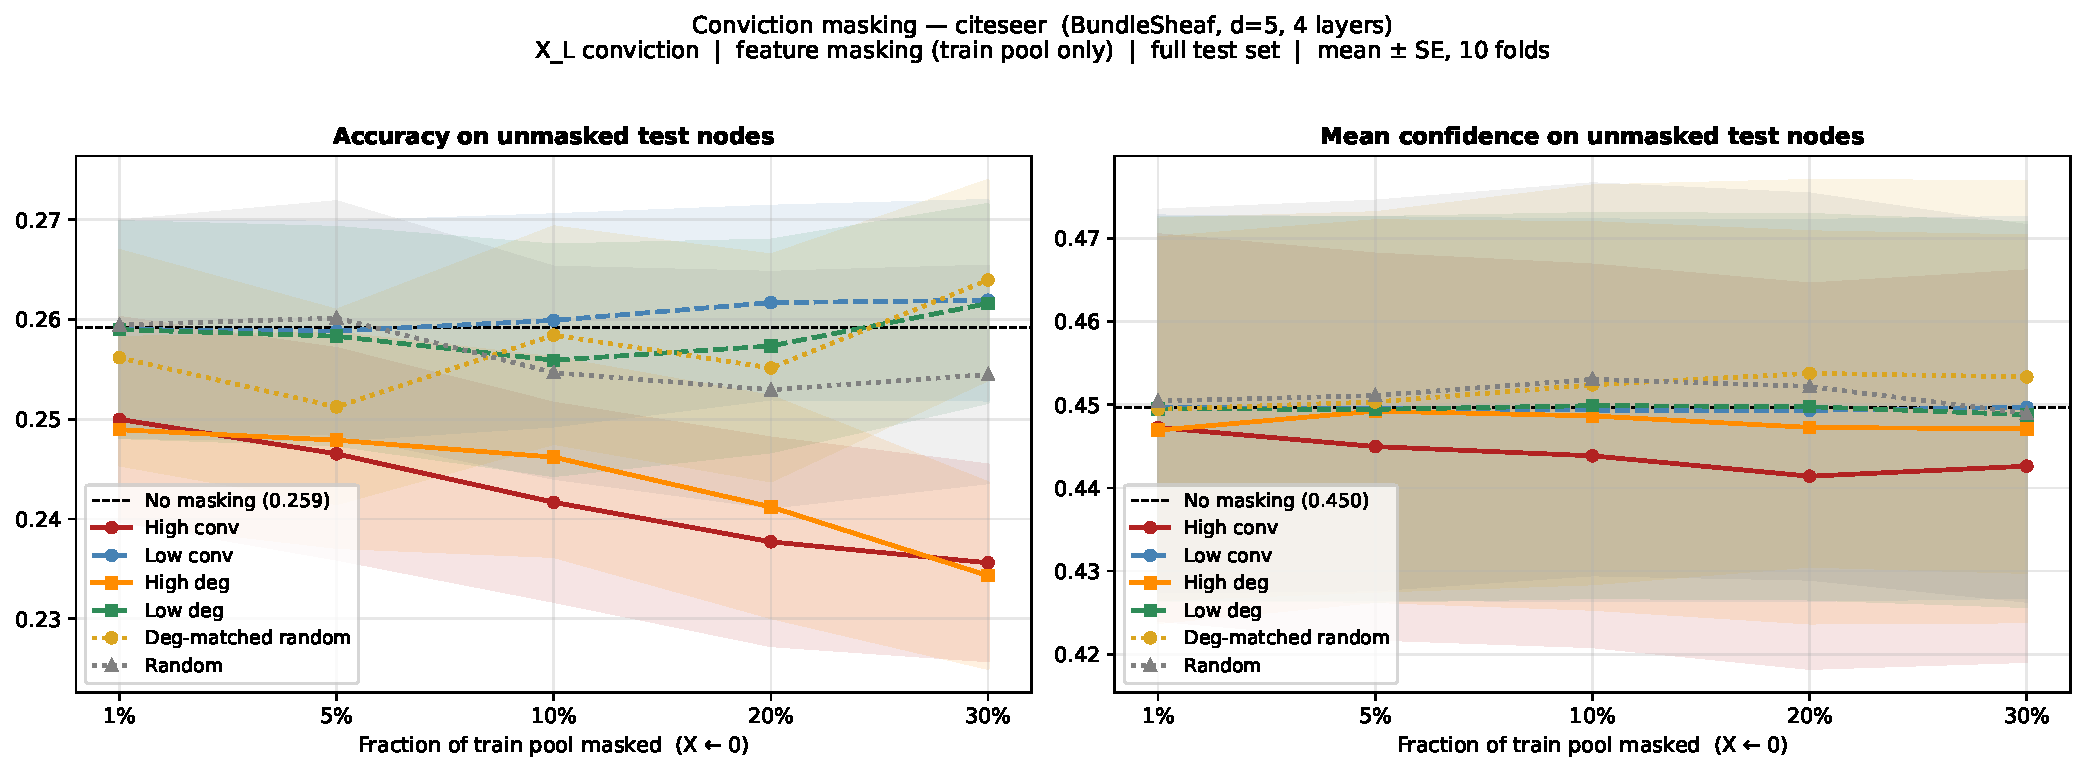
\includegraphics[width=\linewidth]{accuracy_ranking/BundleSheaf/normalised_false/citeseer_BundleSheaf_d5_4L_Norm_False_conviction_masking.pdf}
\end{figure}
\end{frame}

\begin{frame}{Cora --- BundleSheaf, $d=5$, $L=3$, Norm=False}
\begin{figure}
    \centering
    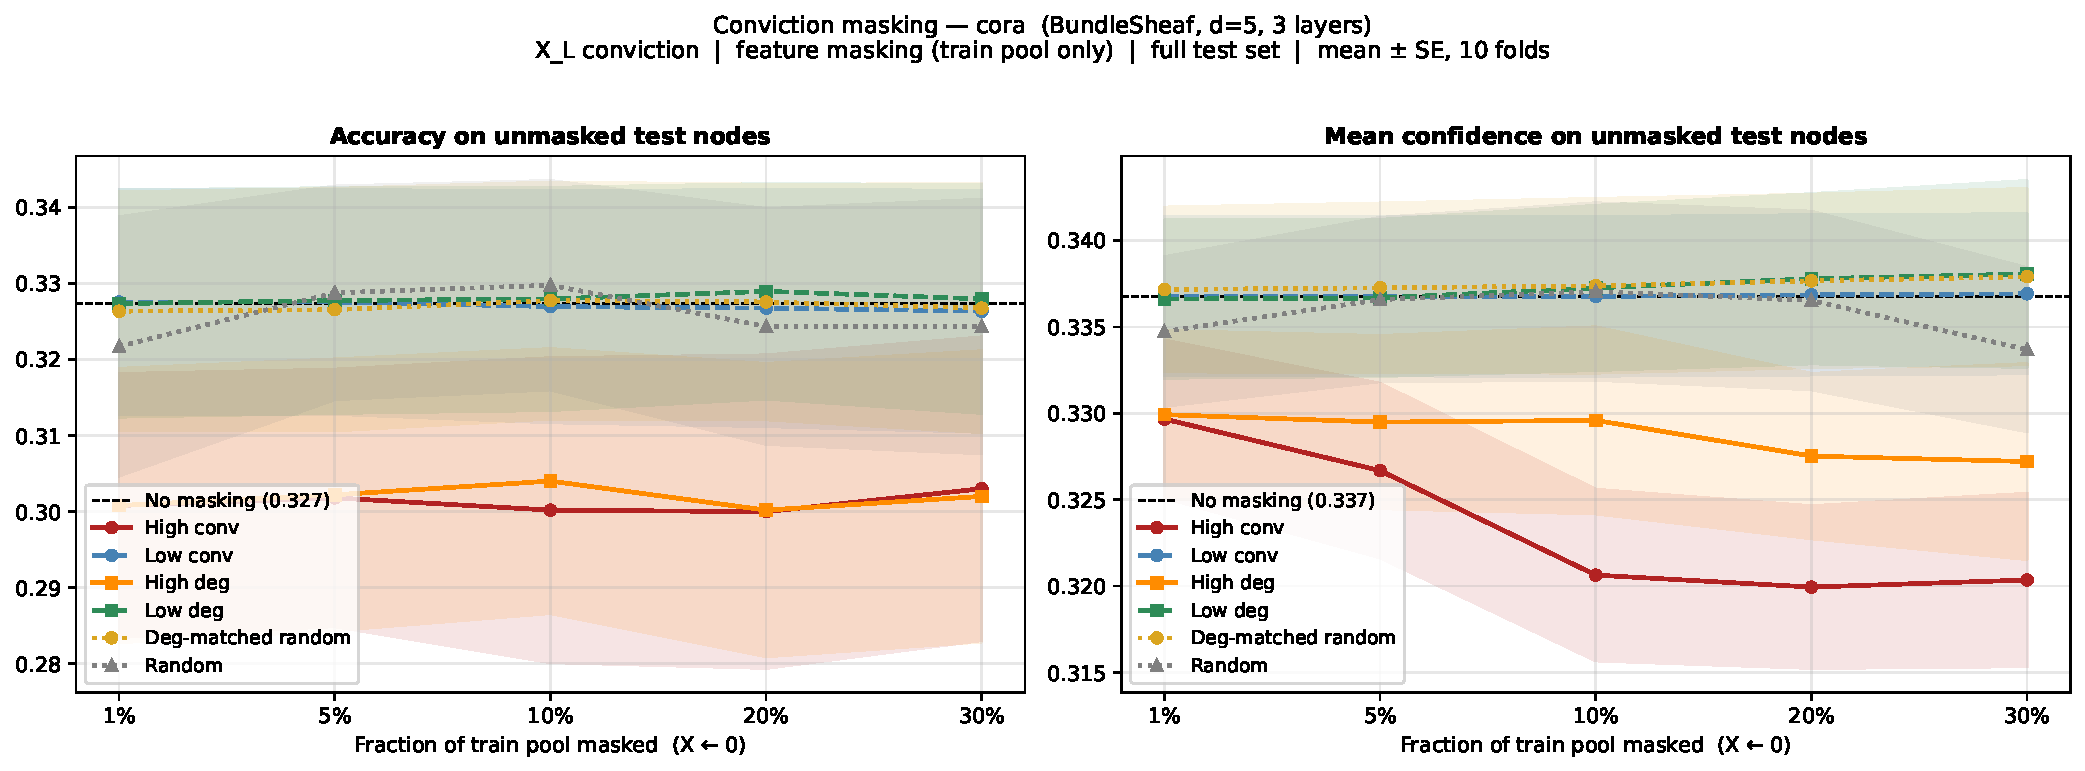
\includegraphics[width=\linewidth]{accuracy_ranking/BundleSheaf/normalised_false/cora_BundleSheaf_d5_3L_Norm_False_conviction_masking.pdf}
\end{figure}
\end{frame}

\begin{frame}{Cornell --- BundleSheaf, $d=2$, $L=2$, Norm=False}
\begin{figure}
    \centering
    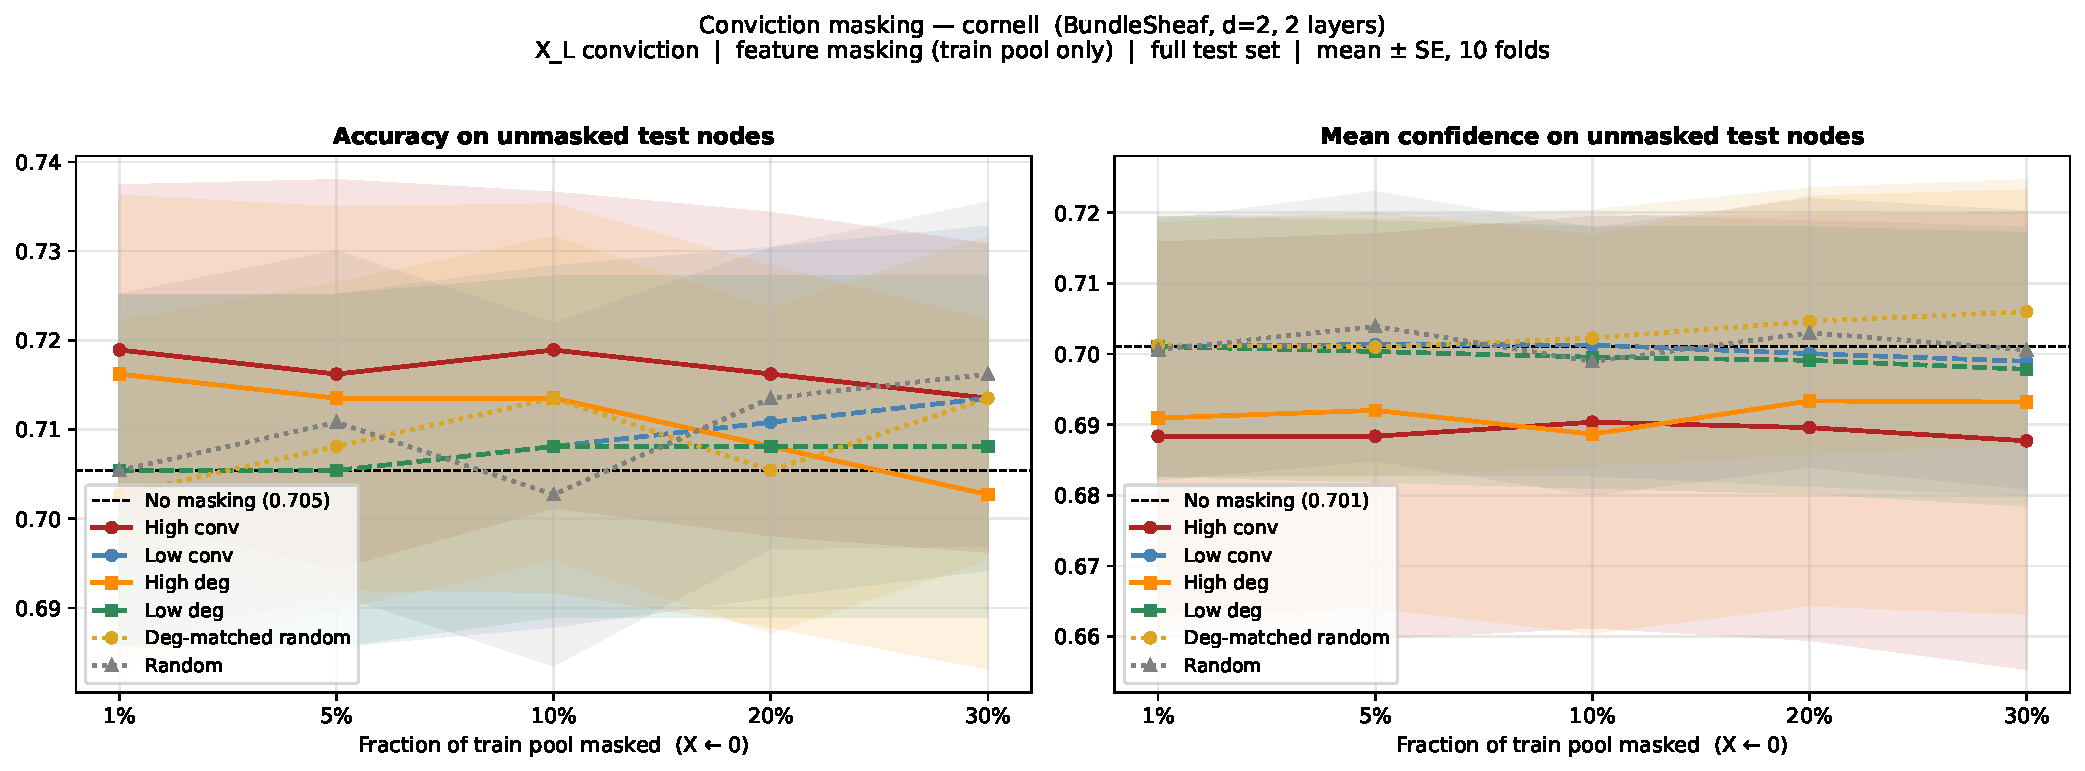
\includegraphics[width=0.8\linewidth]{accuracy_ranking/BundleSheaf/normalised_false/cornell_BundleSheaf_d2_2L_Norm_False_conviction_masking.pdf}
\end{figure}
\end{frame}

\begin{frame}{Minesweeper --- BundleSheaf, $d=5$, $L=6$, Norm=False}
\begin{figure}
    \centering
    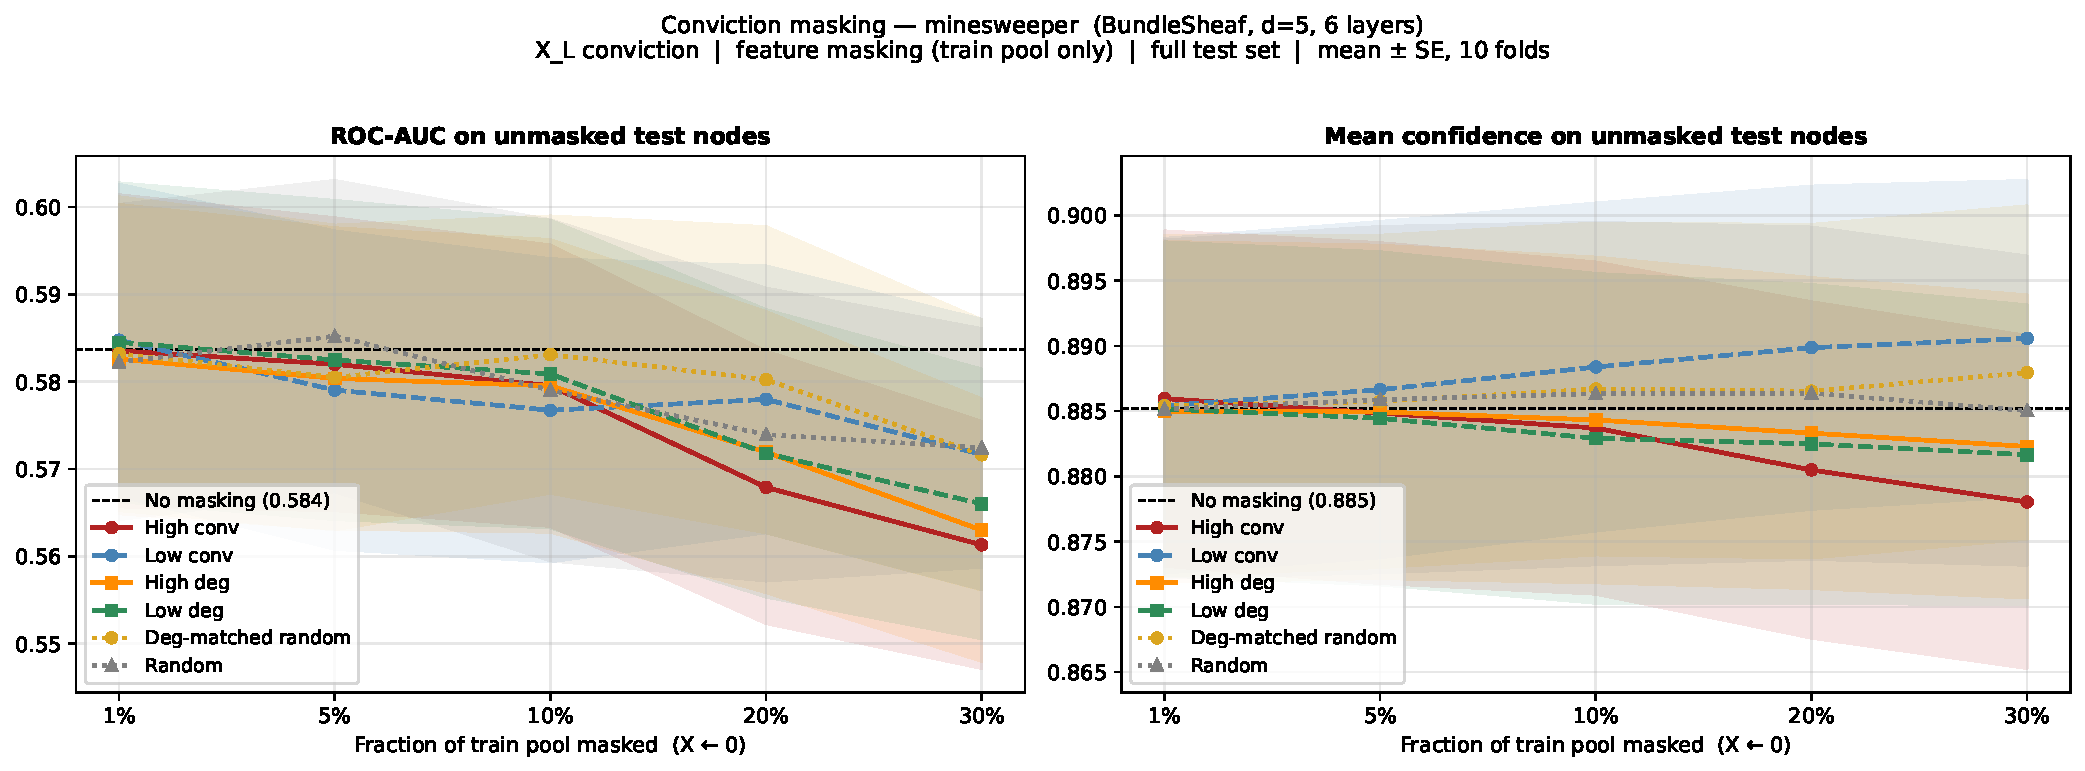
\includegraphics[width=\linewidth]{accuracy_ranking/BundleSheaf/normalised_false/minesweeper_BundleSheaf_d5_6L_Norm_False_conviction_masking.pdf}
\end{figure}
\end{frame}

\begin{frame}{Pubmed --- BundleSheaf, $d=5$, $L=4$, Norm=False}
\begin{figure}
    \centering
    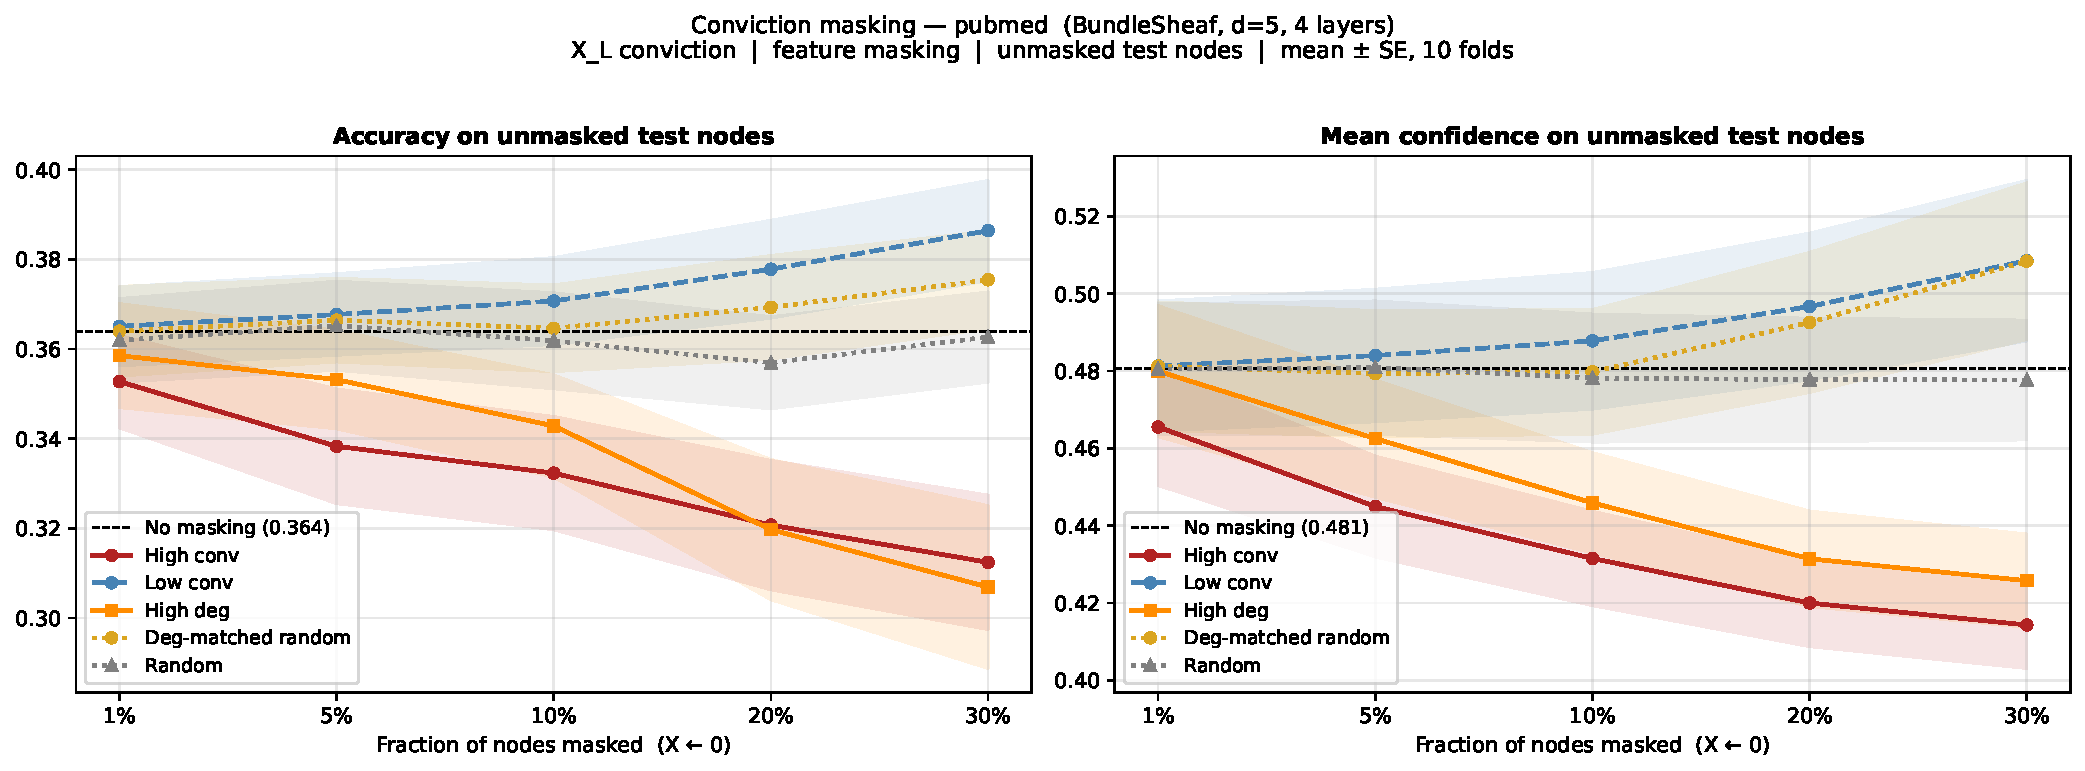
\includegraphics[width=\linewidth]{accuracy_ranking/BundleSheaf/normalised_false/pubmed_BundleSheaf_d5_4L_Norm_False_conviction_masking.pdf}
\end{figure}
\end{frame}

\begin{frame}{Questions --- BundleSheaf, $d=5$, $L=4$, Norm=False}
\begin{figure}
    \centering
    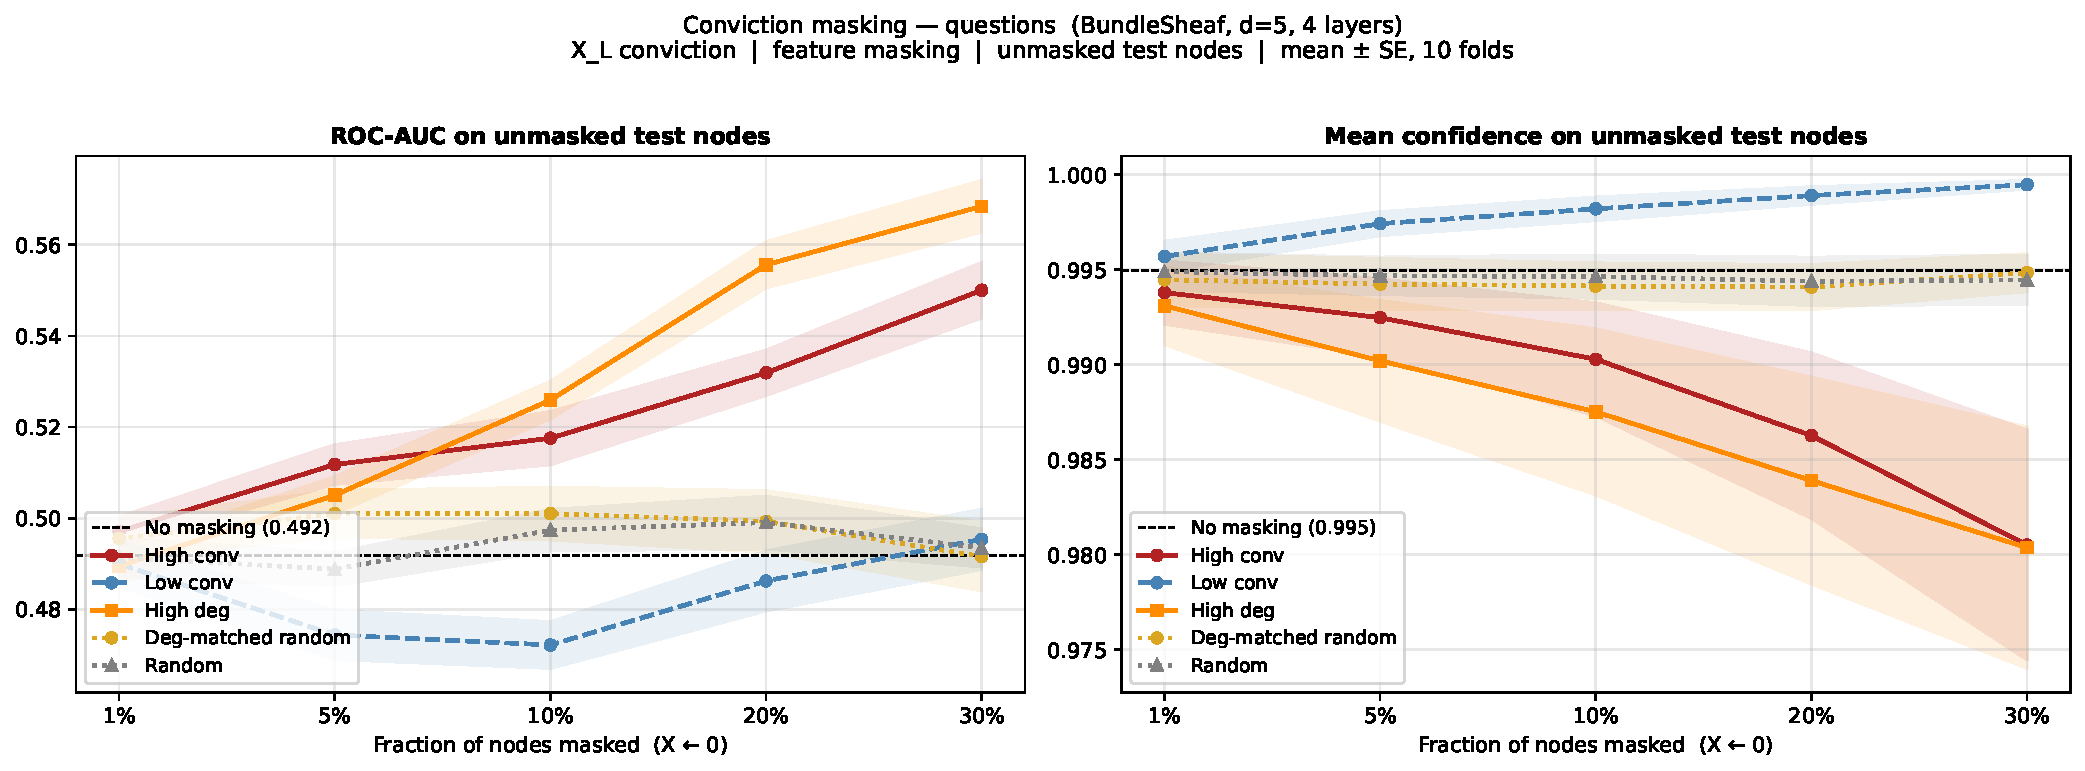
\includegraphics[width=\linewidth]{accuracy_ranking/BundleSheaf/normalised_false/questions_BundleSheaf_d5_4L_Norm_False_conviction_masking.pdf}
\end{figure}
\end{frame}

\begin{frame}{Roman Empire --- BundleSheaf, $d=5$, $L=5$, Norm=False}
\begin{figure}
    \centering
    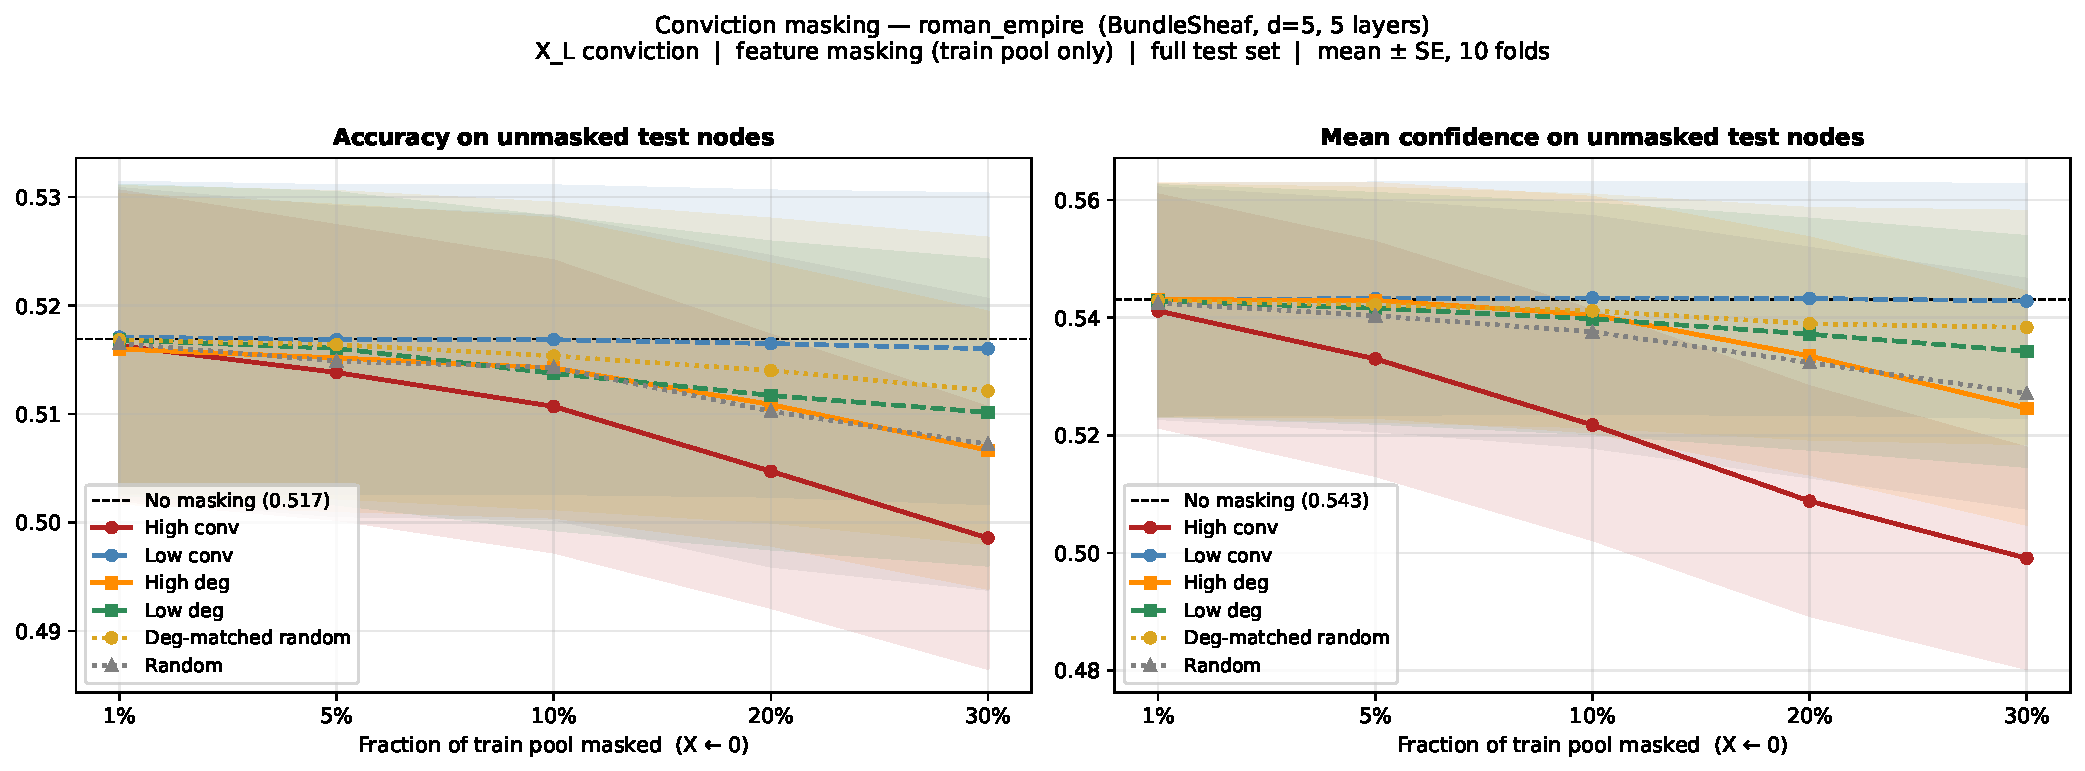
\includegraphics[width=\linewidth]{accuracy_ranking/BundleSheaf/normalised_false/roman_empire_BundleSheaf_d5_5L_Norm_False_conviction_masking.pdf}
\end{figure}
\end{frame}

\begin{frame}{Tolokers --- BundleSheaf, $d=3$, $L=4$, Norm=False}
\begin{figure}
    \centering
    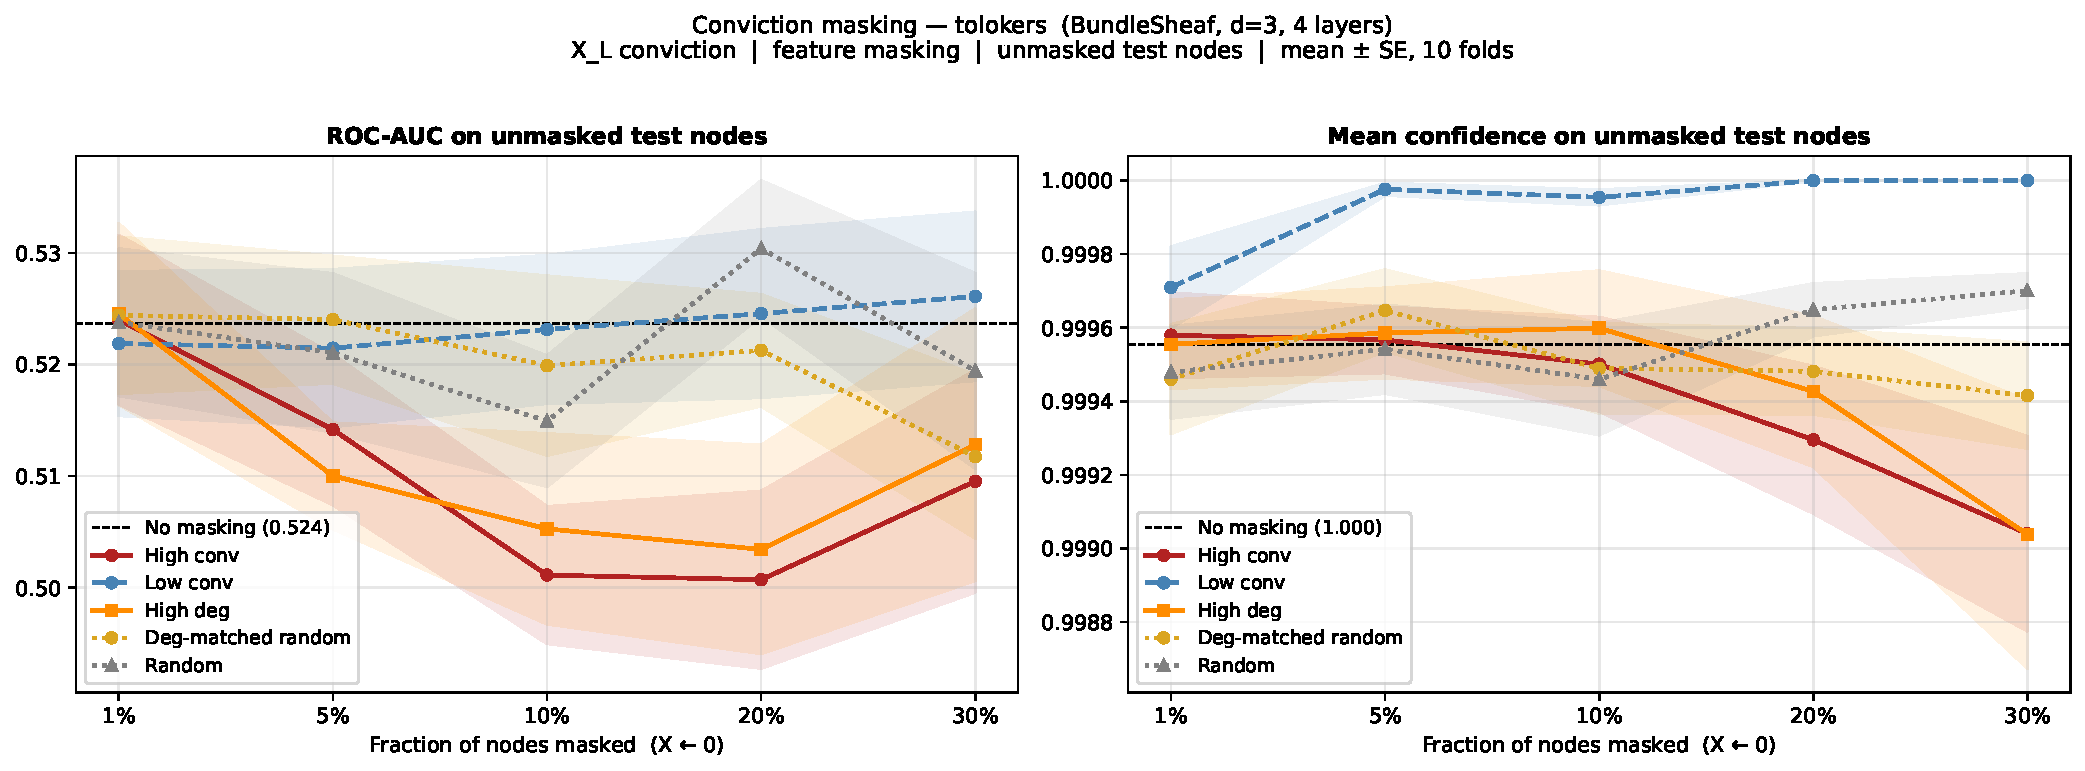
\includegraphics[width=\linewidth]{accuracy_ranking/BundleSheaf/normalised_false/tolokers_BundleSheaf_d3_4L_Norm_False_conviction_masking.pdf}
\end{figure}
\end{frame}

\begin{frame}{Wisconsin --- BundleSheaf, $d=2$, $L=2$, Norm=False}
\begin{figure}
    \centering
    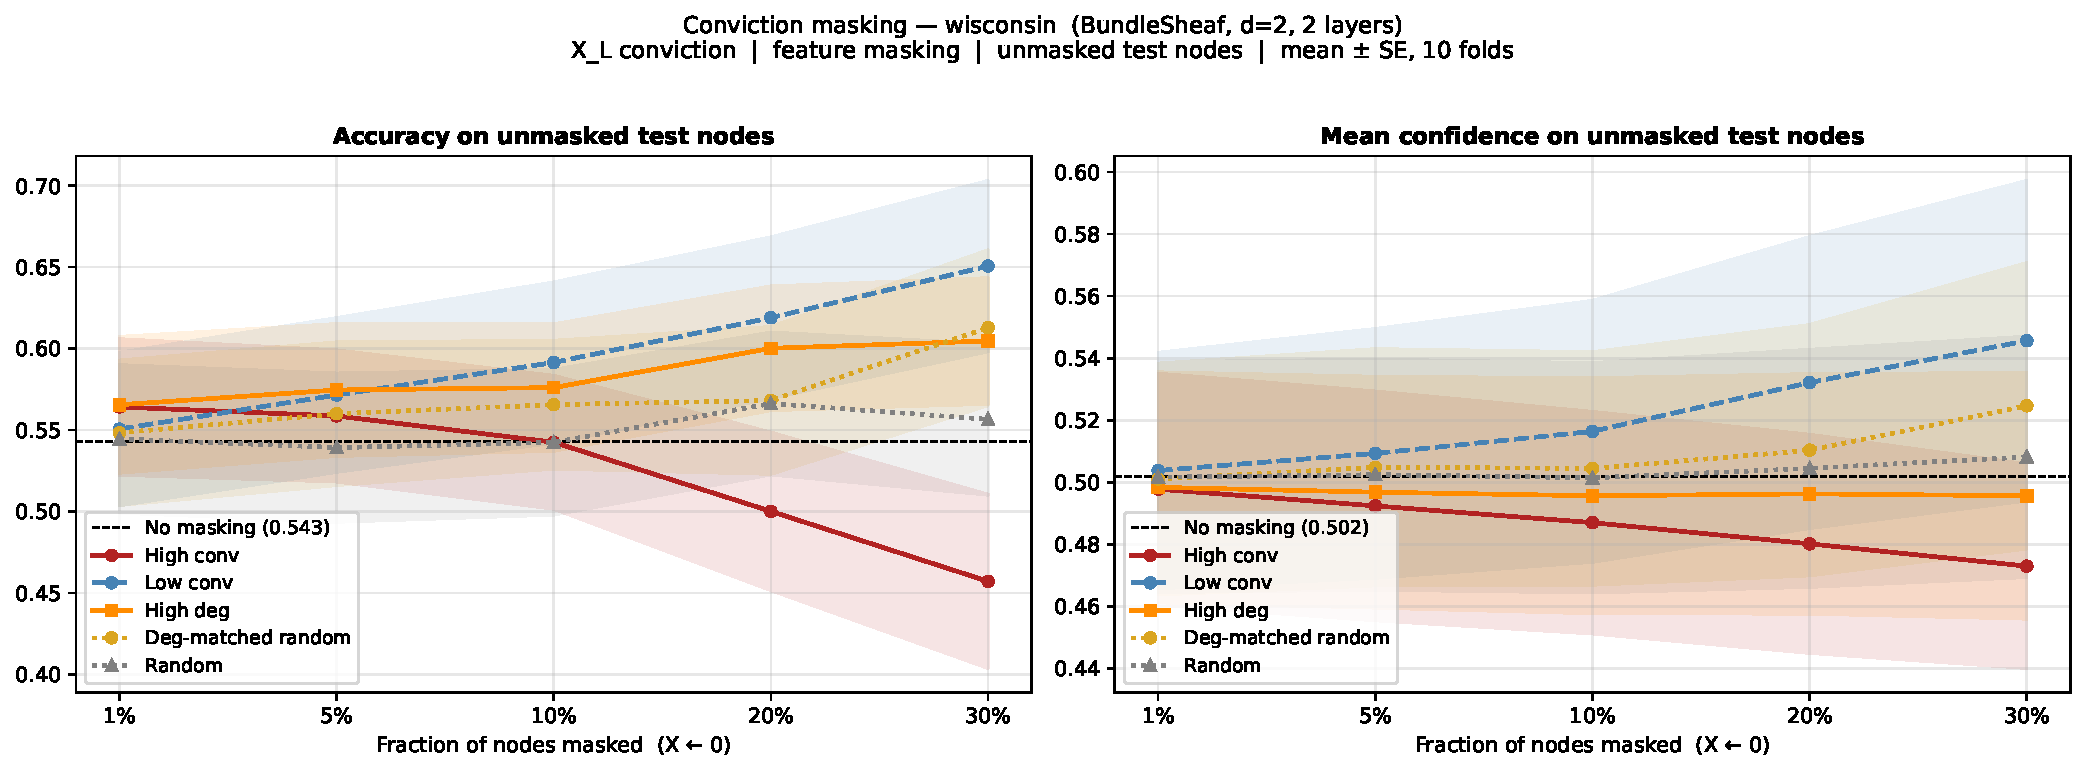
\includegraphics[width=0.8\linewidth]{accuracy_ranking/BundleSheaf/normalised_false/wisconsin_BundleSheaf_d2_2L_Norm_False_conviction_masking.pdf}
\end{figure}
\end{frame}




% ══════════════════════════════════════════════════════════════════════════════
%  SECTION 5 — Heatmap, BundleSheaf, normalised=False
% ══════════════════════════════════════════════════════════════════════════════

\begin{frame}{}
\centering
\Huge\textbf{Conviction Heatmap}\\[6pt]
\Large BundleSheaf \quad (\texttt{normalised=False})
\end{frame}

\begin{frame}{Amazon Ratings --- BundleSheaf, $d=5$, $L=5$, Norm=False}
\begin{figure}
    \centering
    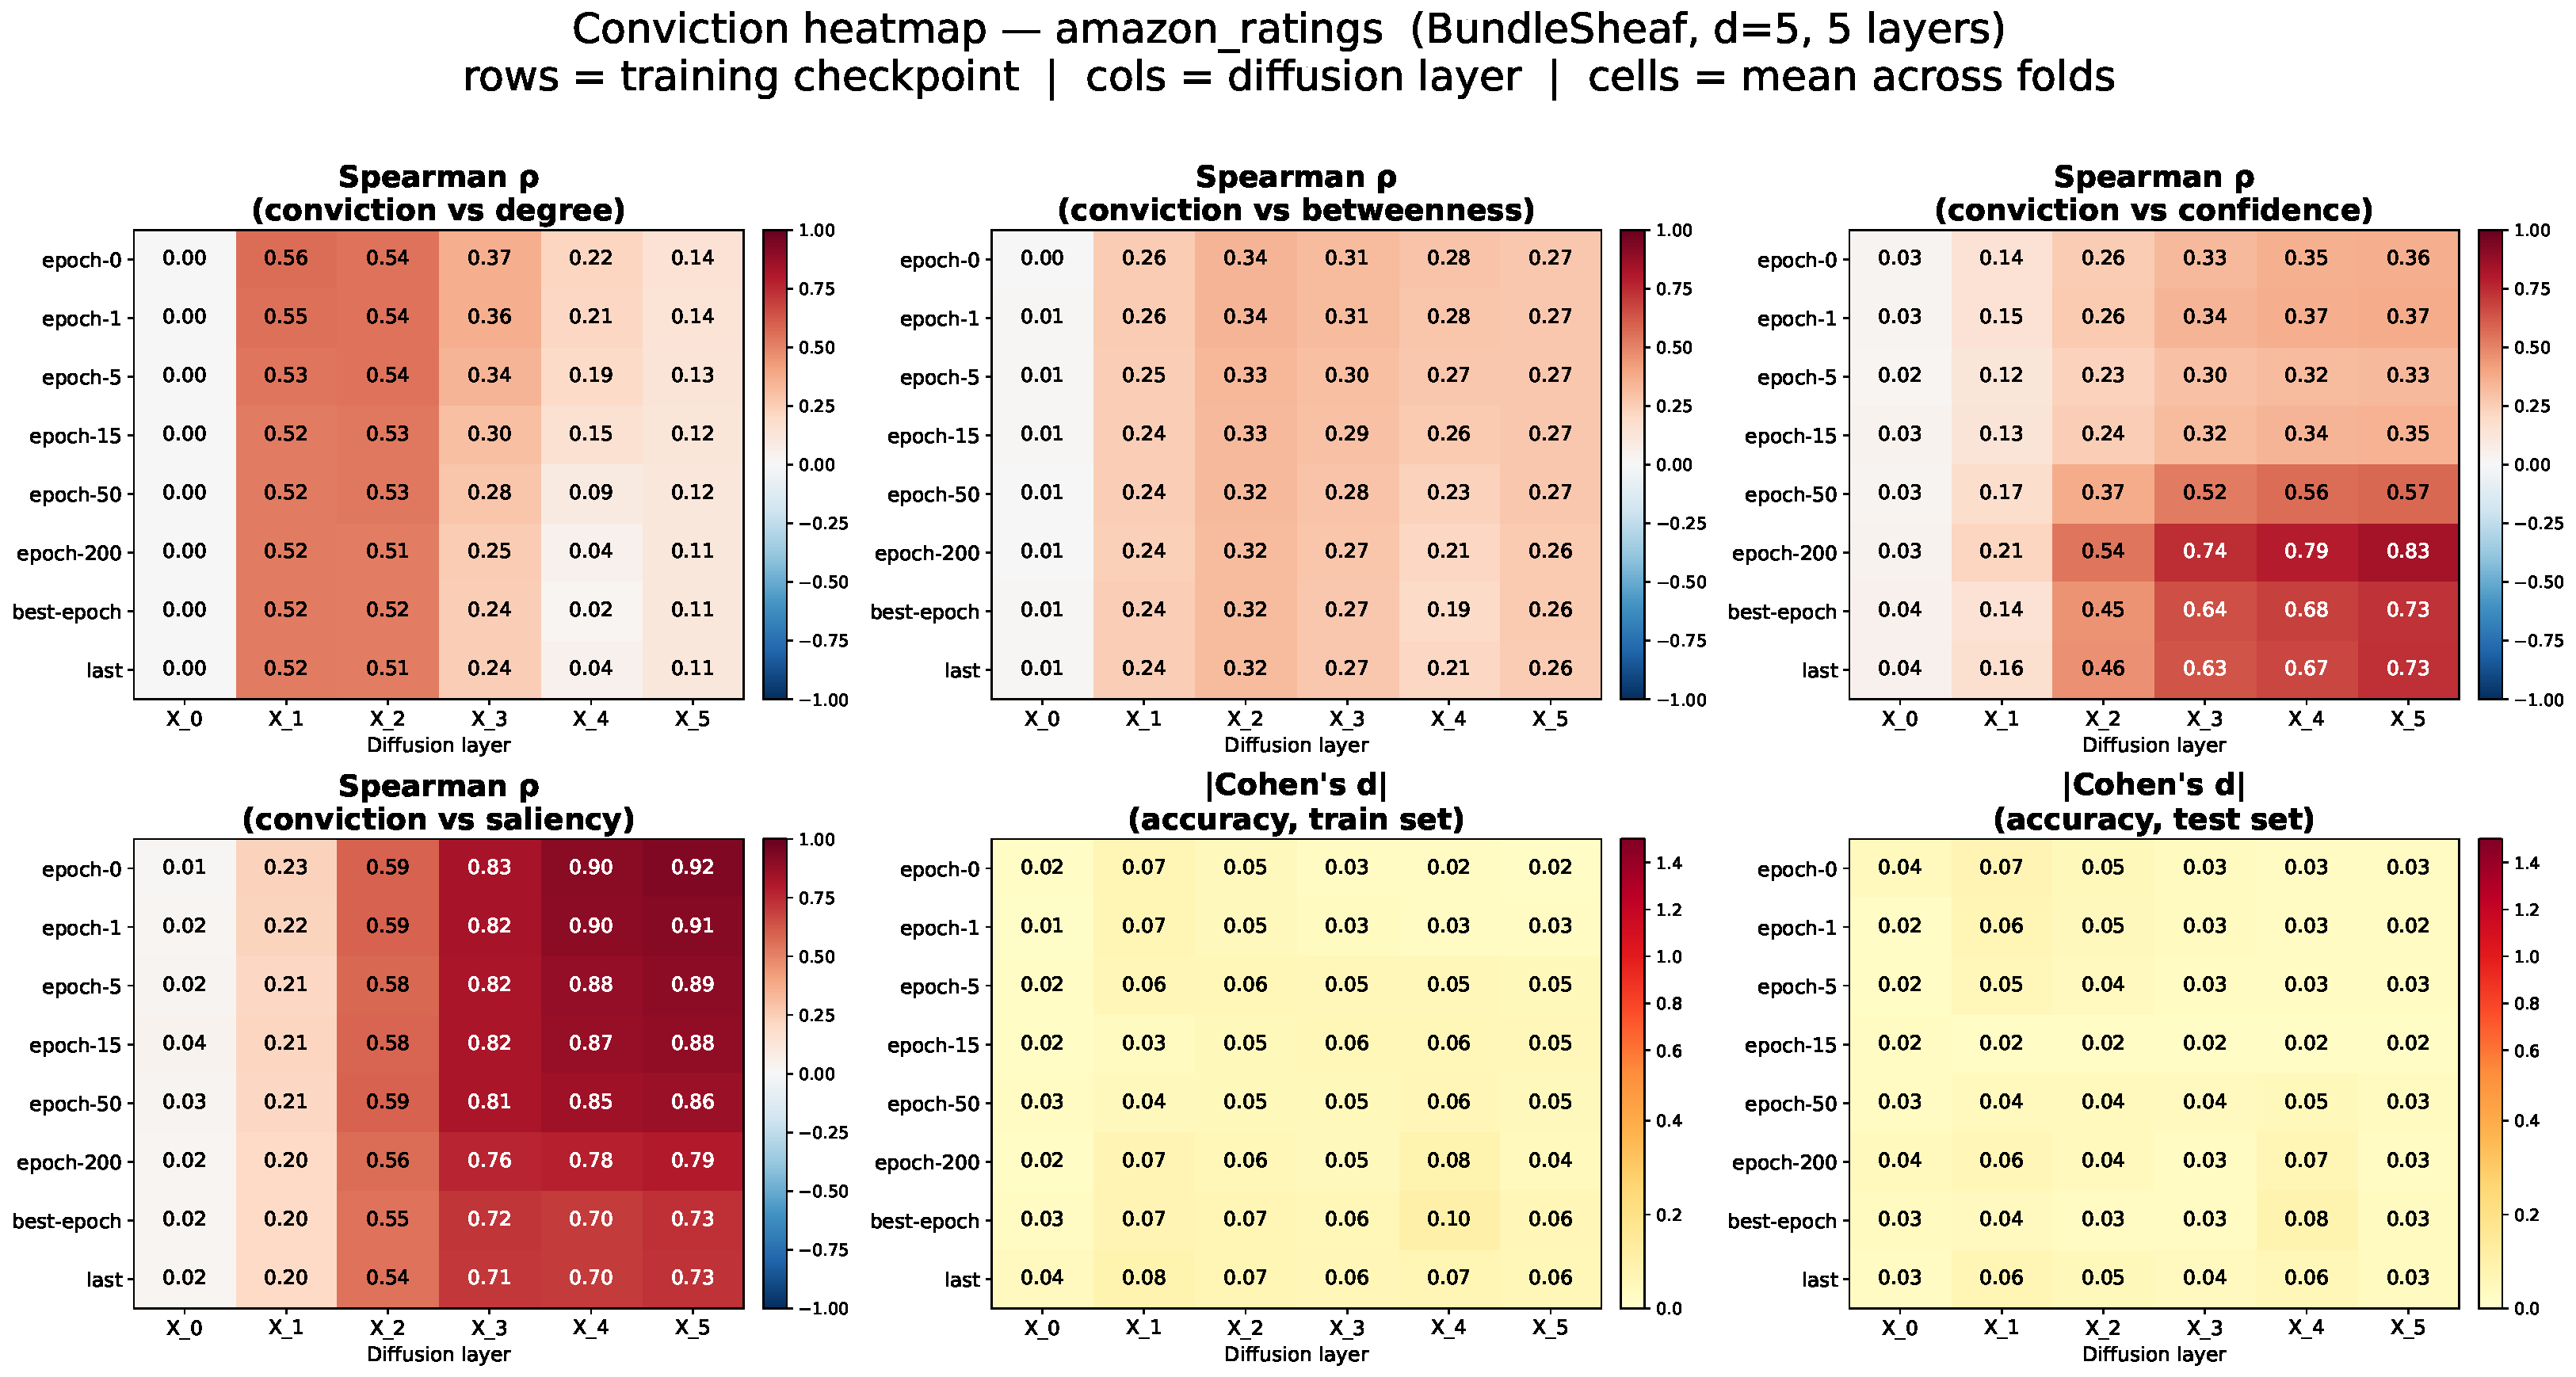
\includegraphics[width=\linewidth]{conviction_heatmap/BundleSheaf/normalised_false/amazon_ratings_BundleSheaf_d5_5L_Norm_False_conviction_heatmap.pdf}
\end{figure}
\end{frame}

\begin{frame}{Citeseer --- BundleSheaf, $d=5$, $L=4$, Norm=False}
\begin{figure}
    \centering
    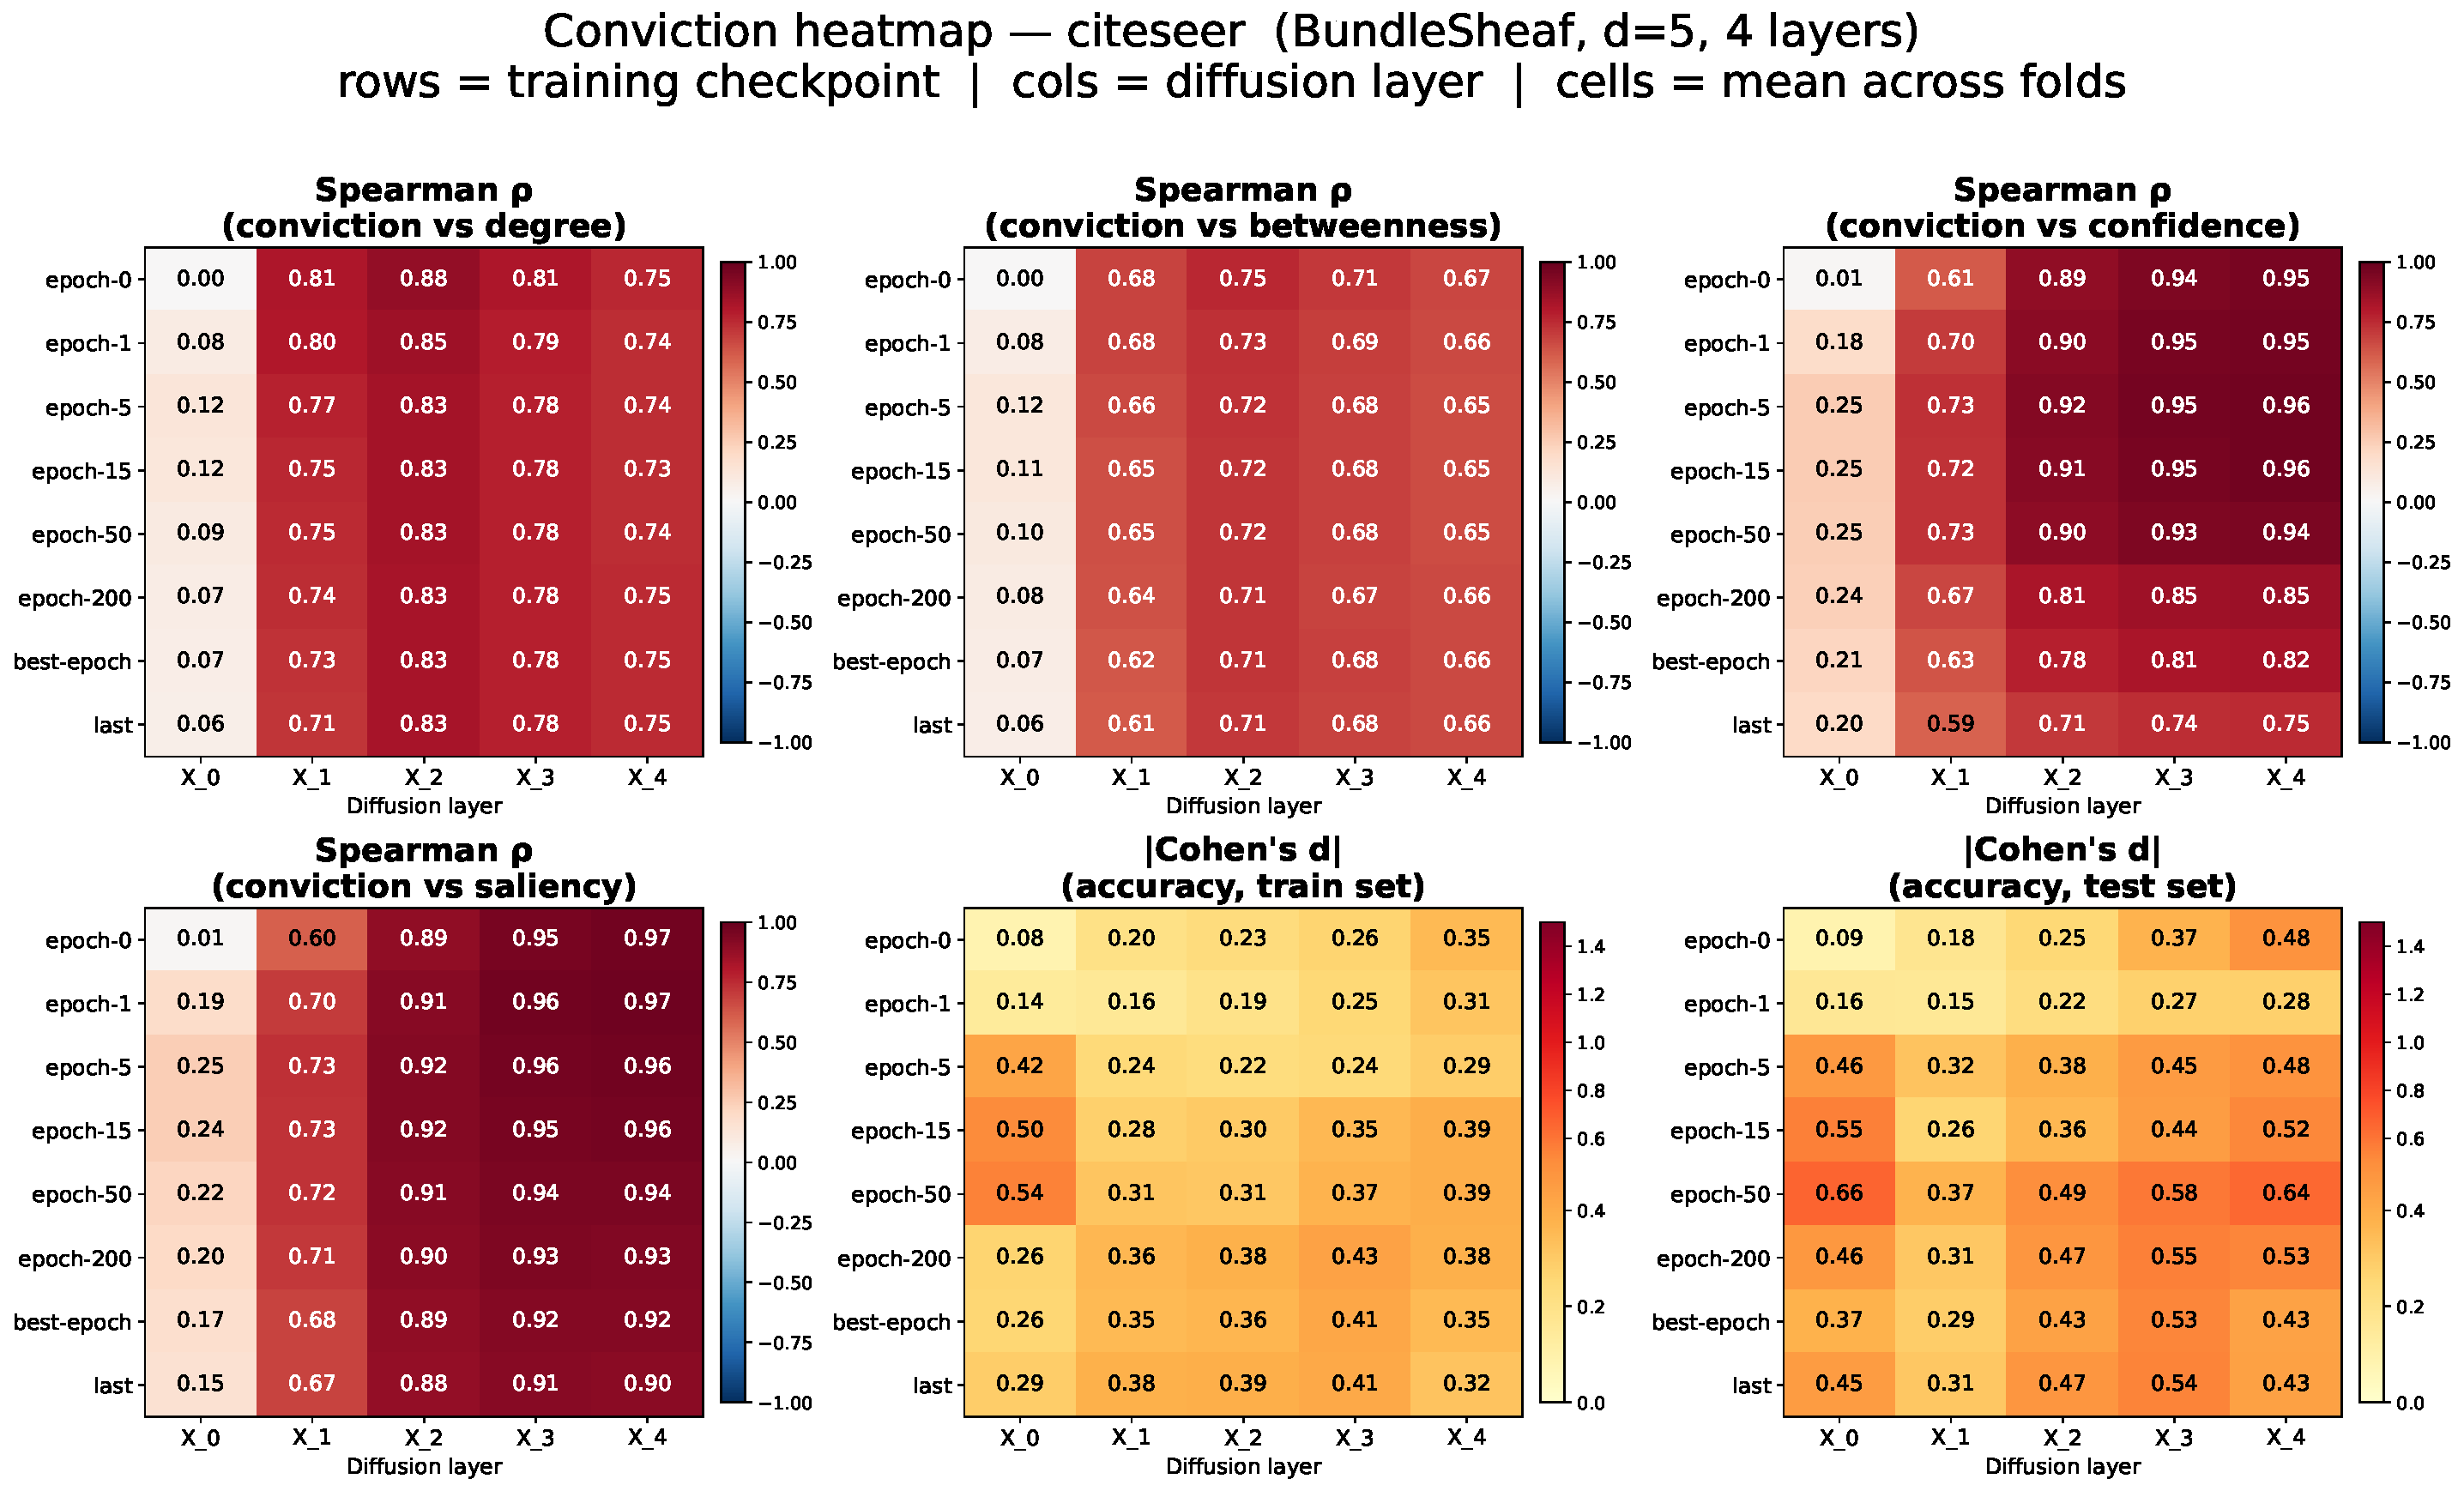
\includegraphics[width=\linewidth]{conviction_heatmap/BundleSheaf/normalised_false/citeseer_BundleSheaf_d5_4L_Norm_False_conviction_heatmap.pdf}
\end{figure}
\end{frame}

\begin{frame}{Cora --- BundleSheaf, $d=5$, $L=3$, Norm=False}
\begin{figure}
    \centering
    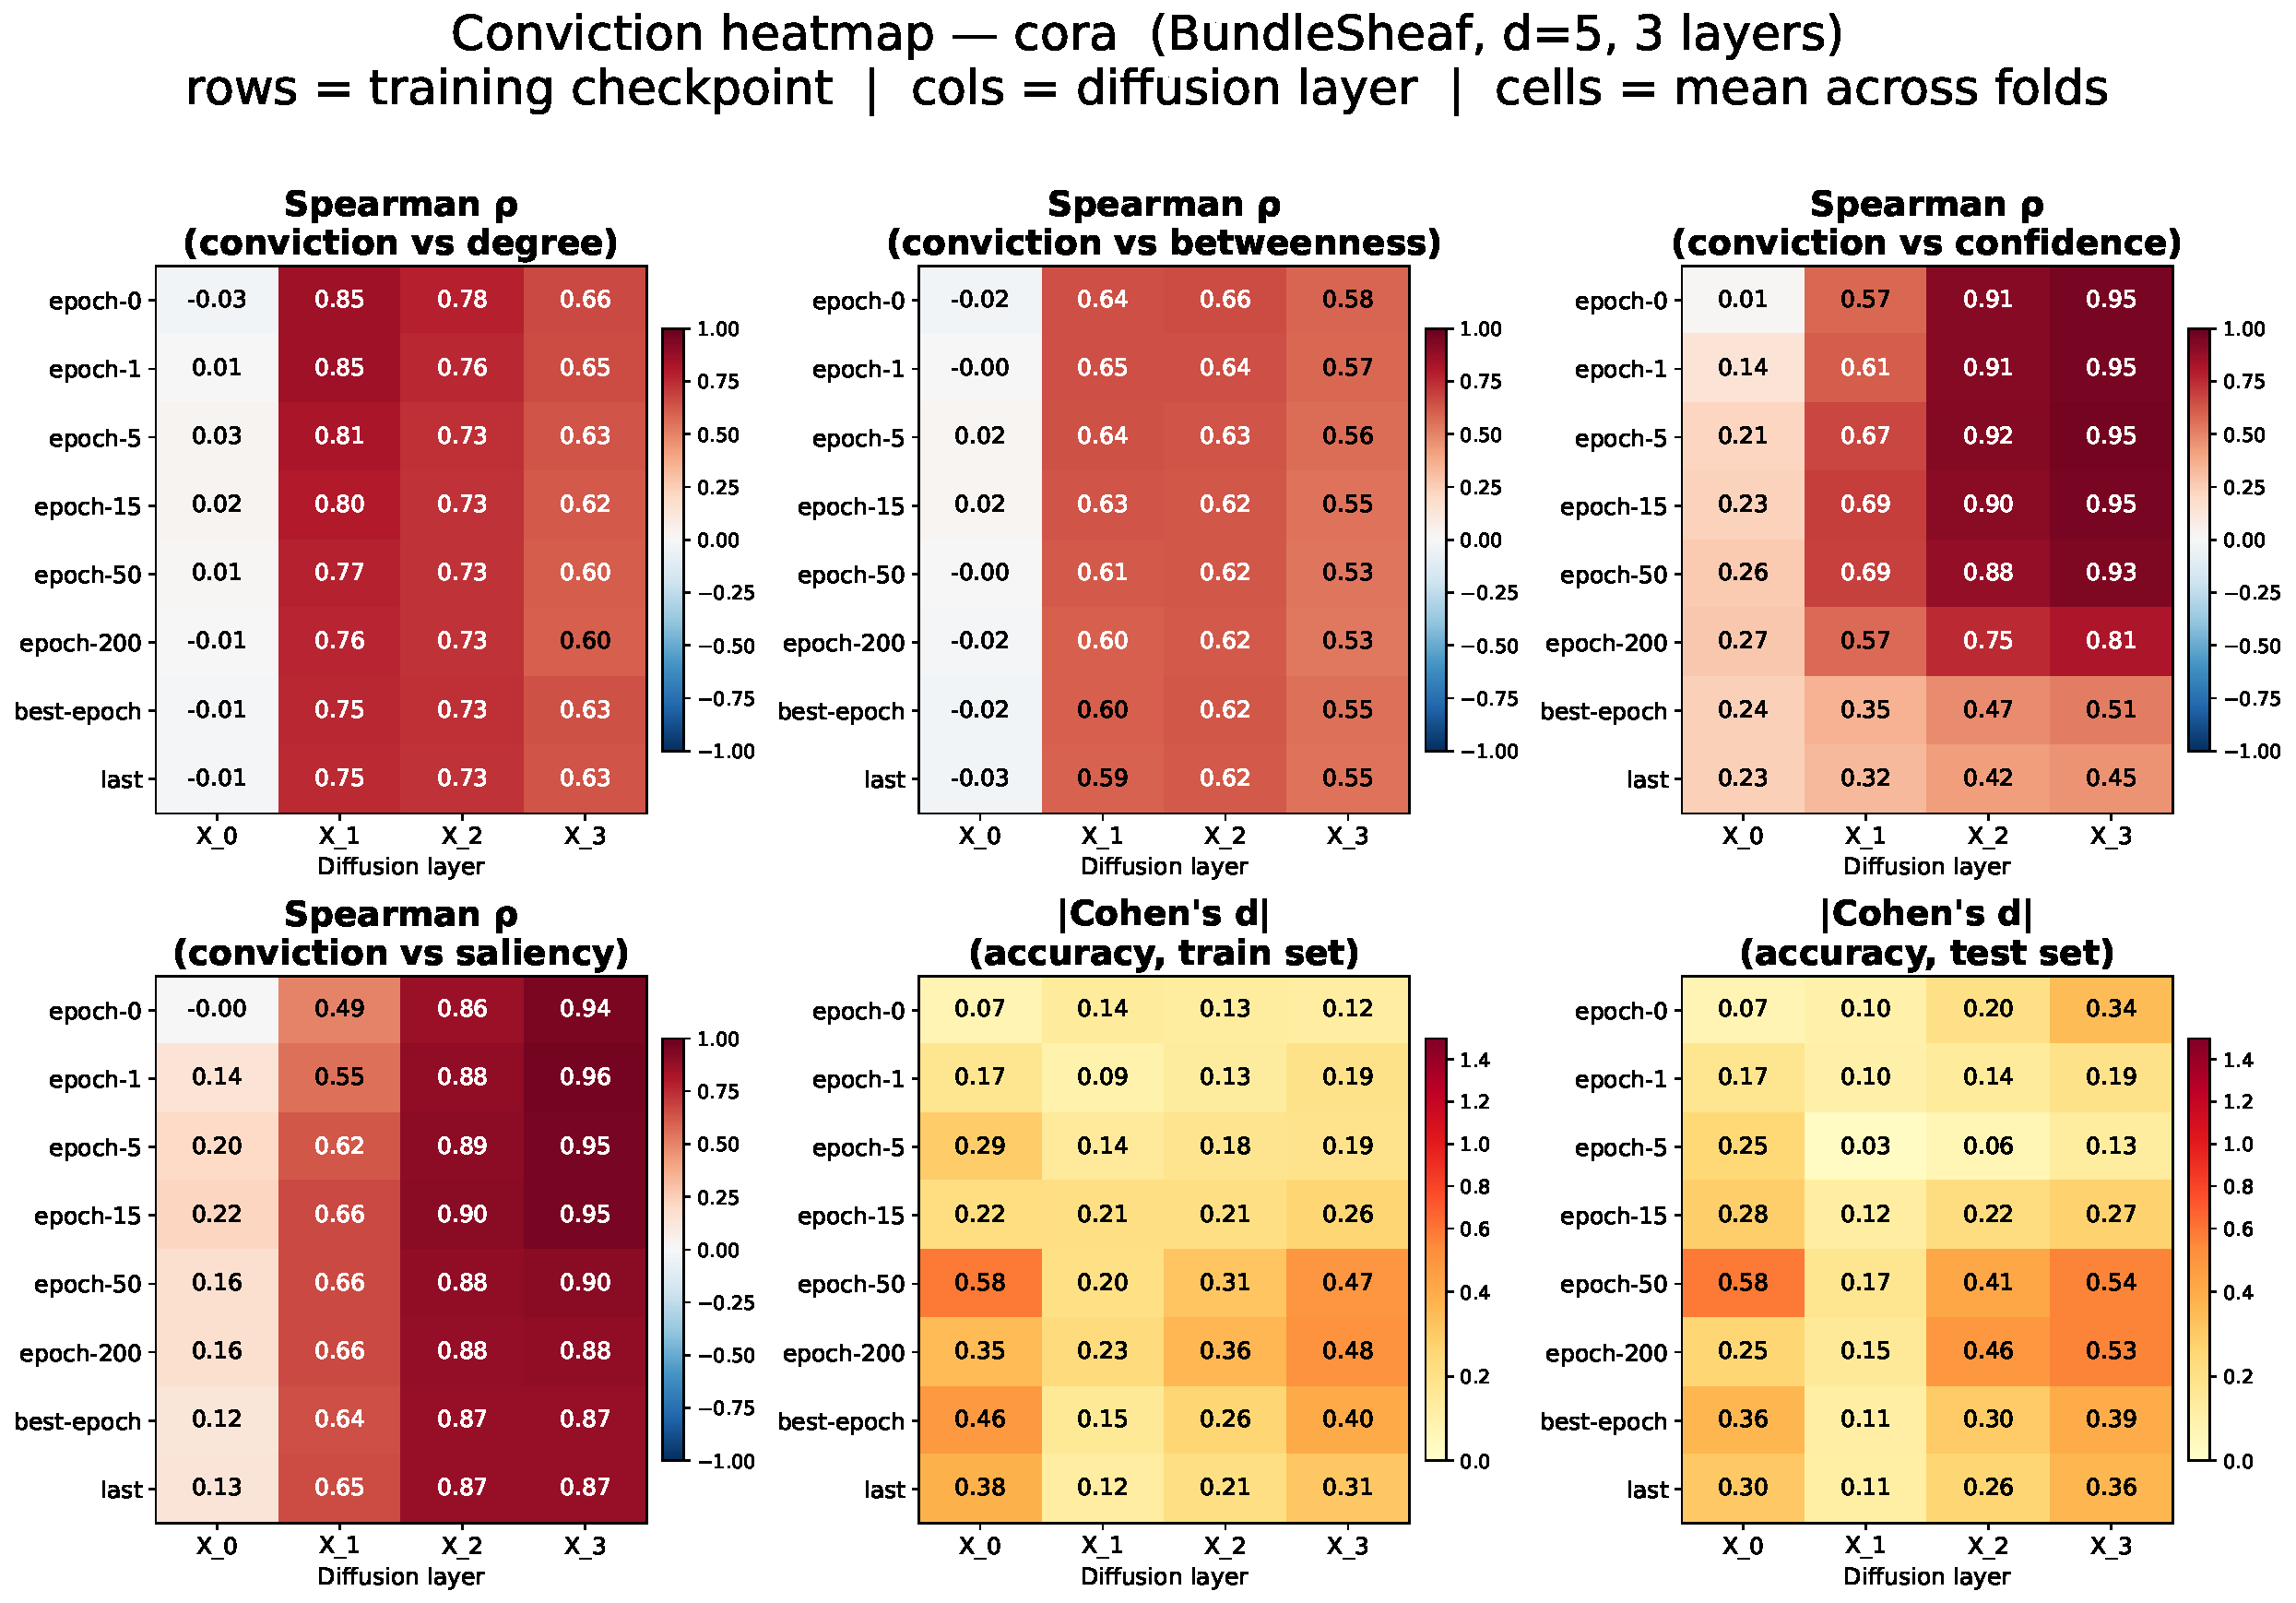
\includegraphics[width=\linewidth]{conviction_heatmap/BundleSheaf/normalised_false/cora_BundleSheaf_d5_3L_Norm_False_conviction_heatmap.pdf}
\end{figure}
\end{frame}

\begin{frame}{Cornell --- BundleSheaf, $d=2$, $L=2$, Norm=False}
\begin{figure}
    \centering
    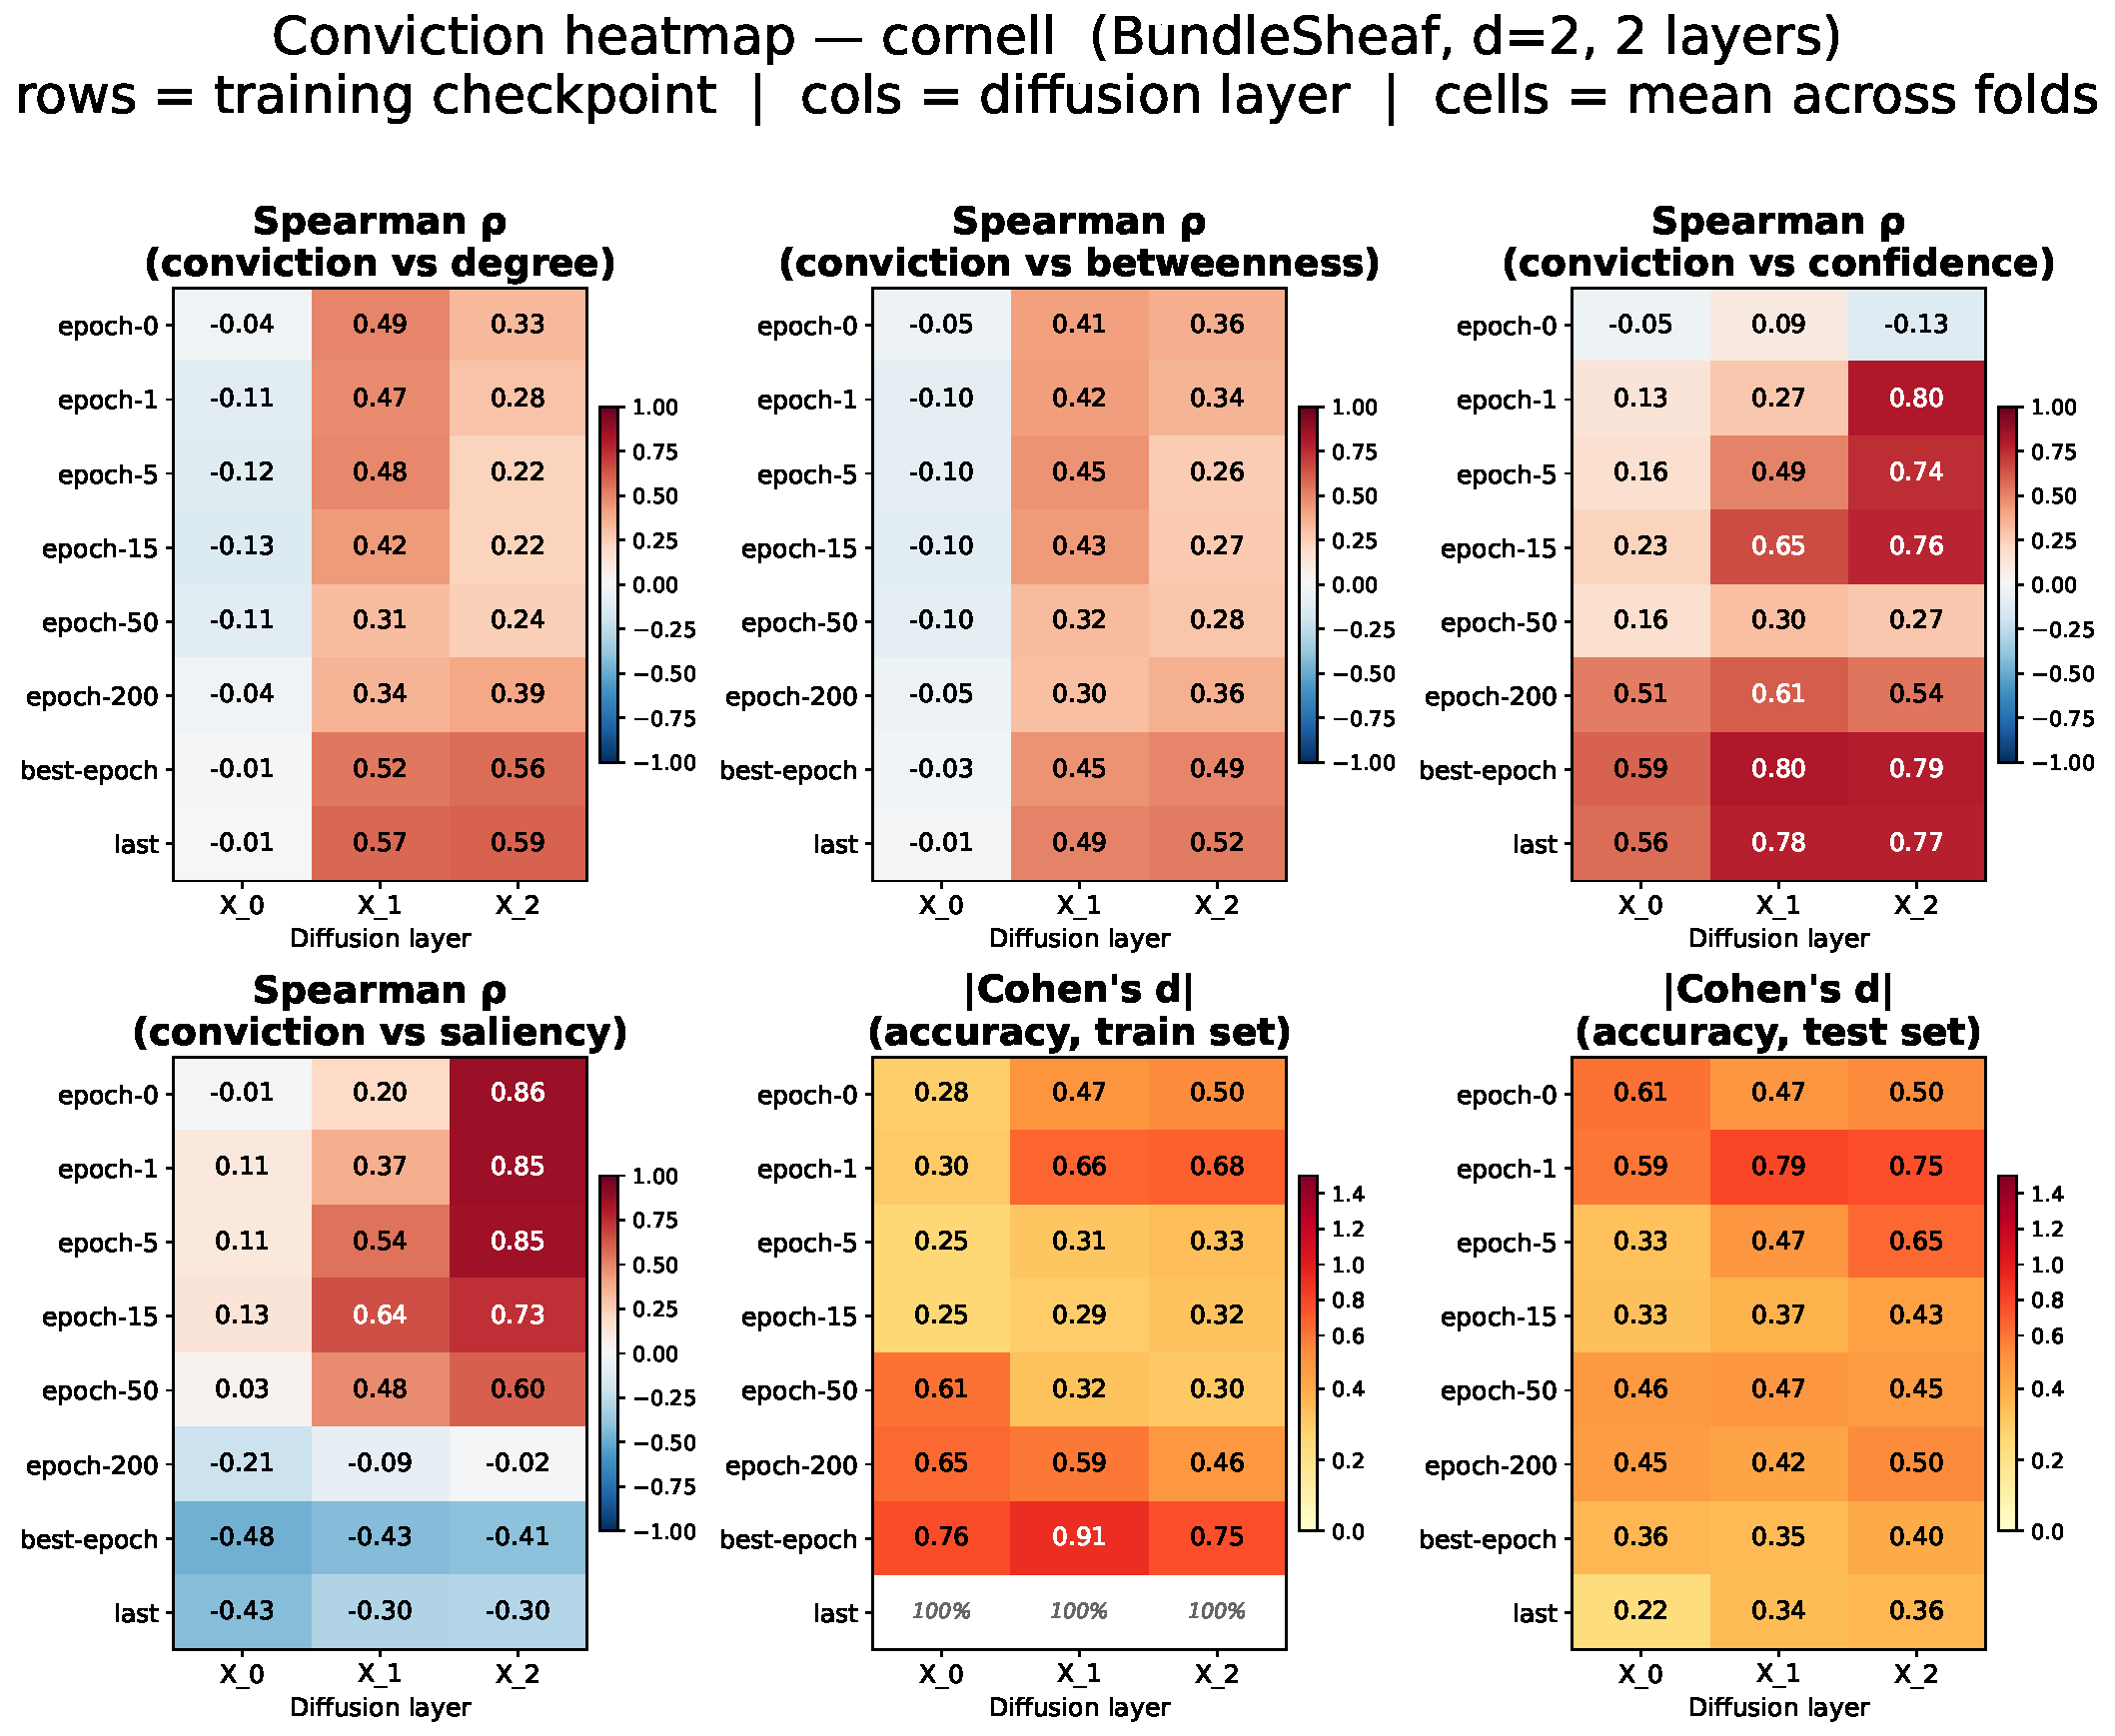
\includegraphics[width=0.8\linewidth]{conviction_heatmap/BundleSheaf/normalised_false/cornell_BundleSheaf_d2_2L_Norm_False_conviction_heatmap.pdf}
\end{figure}
\end{frame}

\begin{frame}{Minesweeper --- BundleSheaf, $d=5$, $L=6$, Norm=False}
\begin{figure}
    \centering
    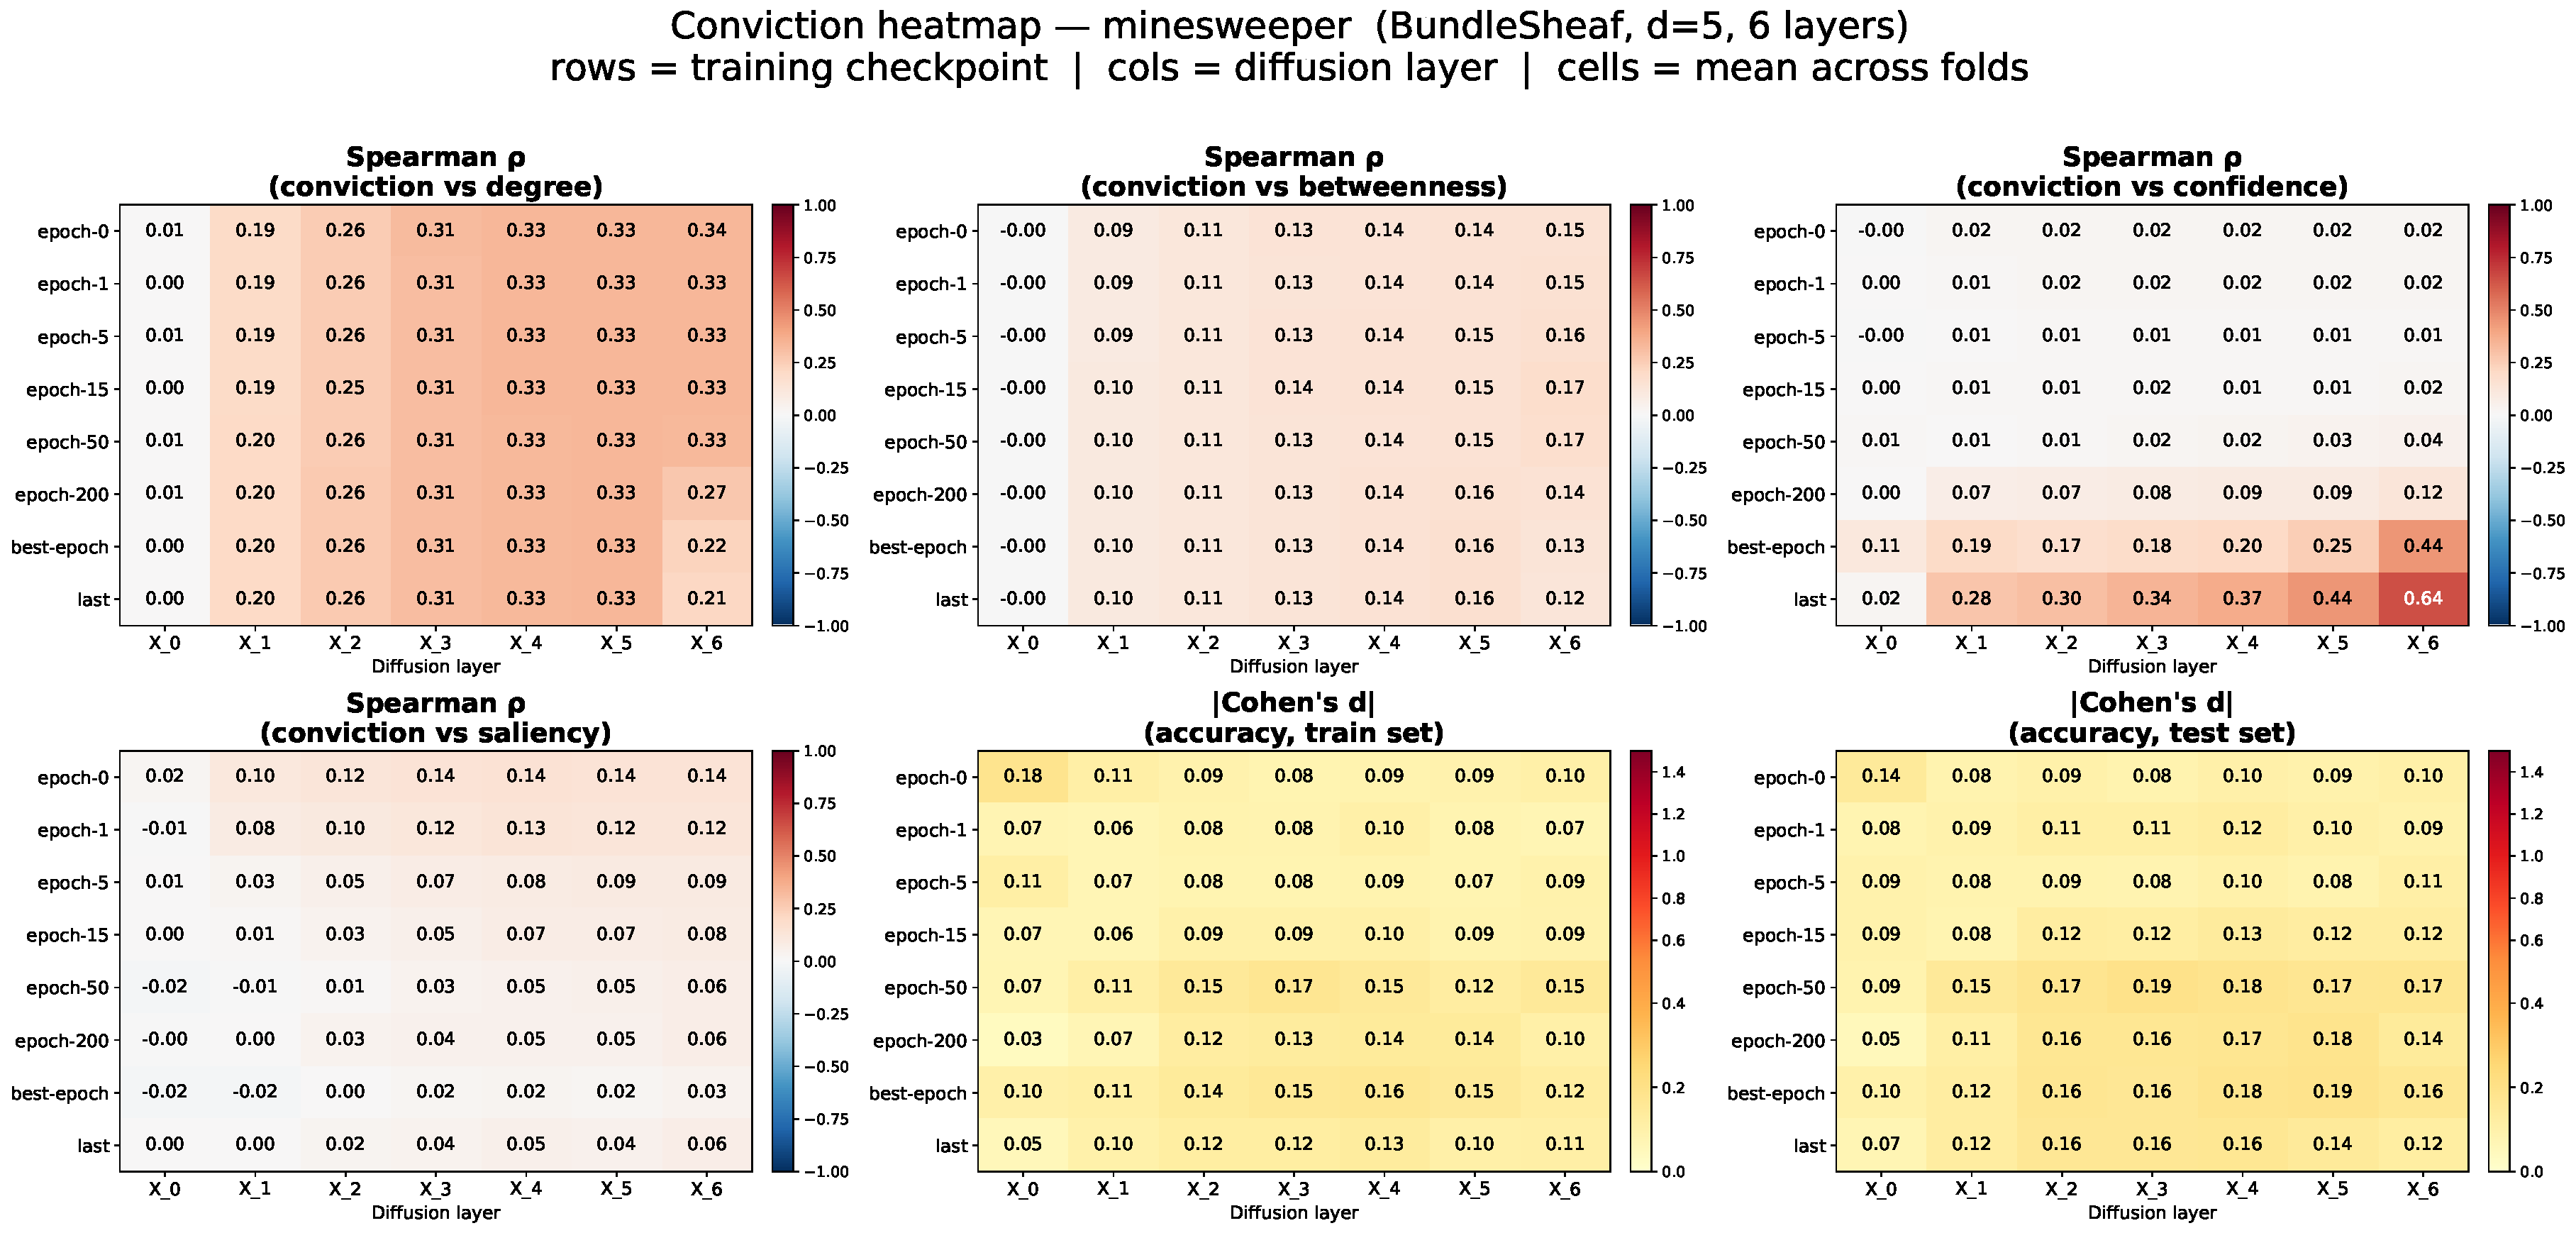
\includegraphics[width=\linewidth]{conviction_heatmap/BundleSheaf/normalised_false/minesweeper_BundleSheaf_d5_6L_Norm_False_conviction_heatmap.pdf}
\end{figure}
\end{frame}

\begin{frame}{Pubmed --- BundleSheaf, $d=5$, $L=4$, Norm=False}
\begin{figure}
    \centering
    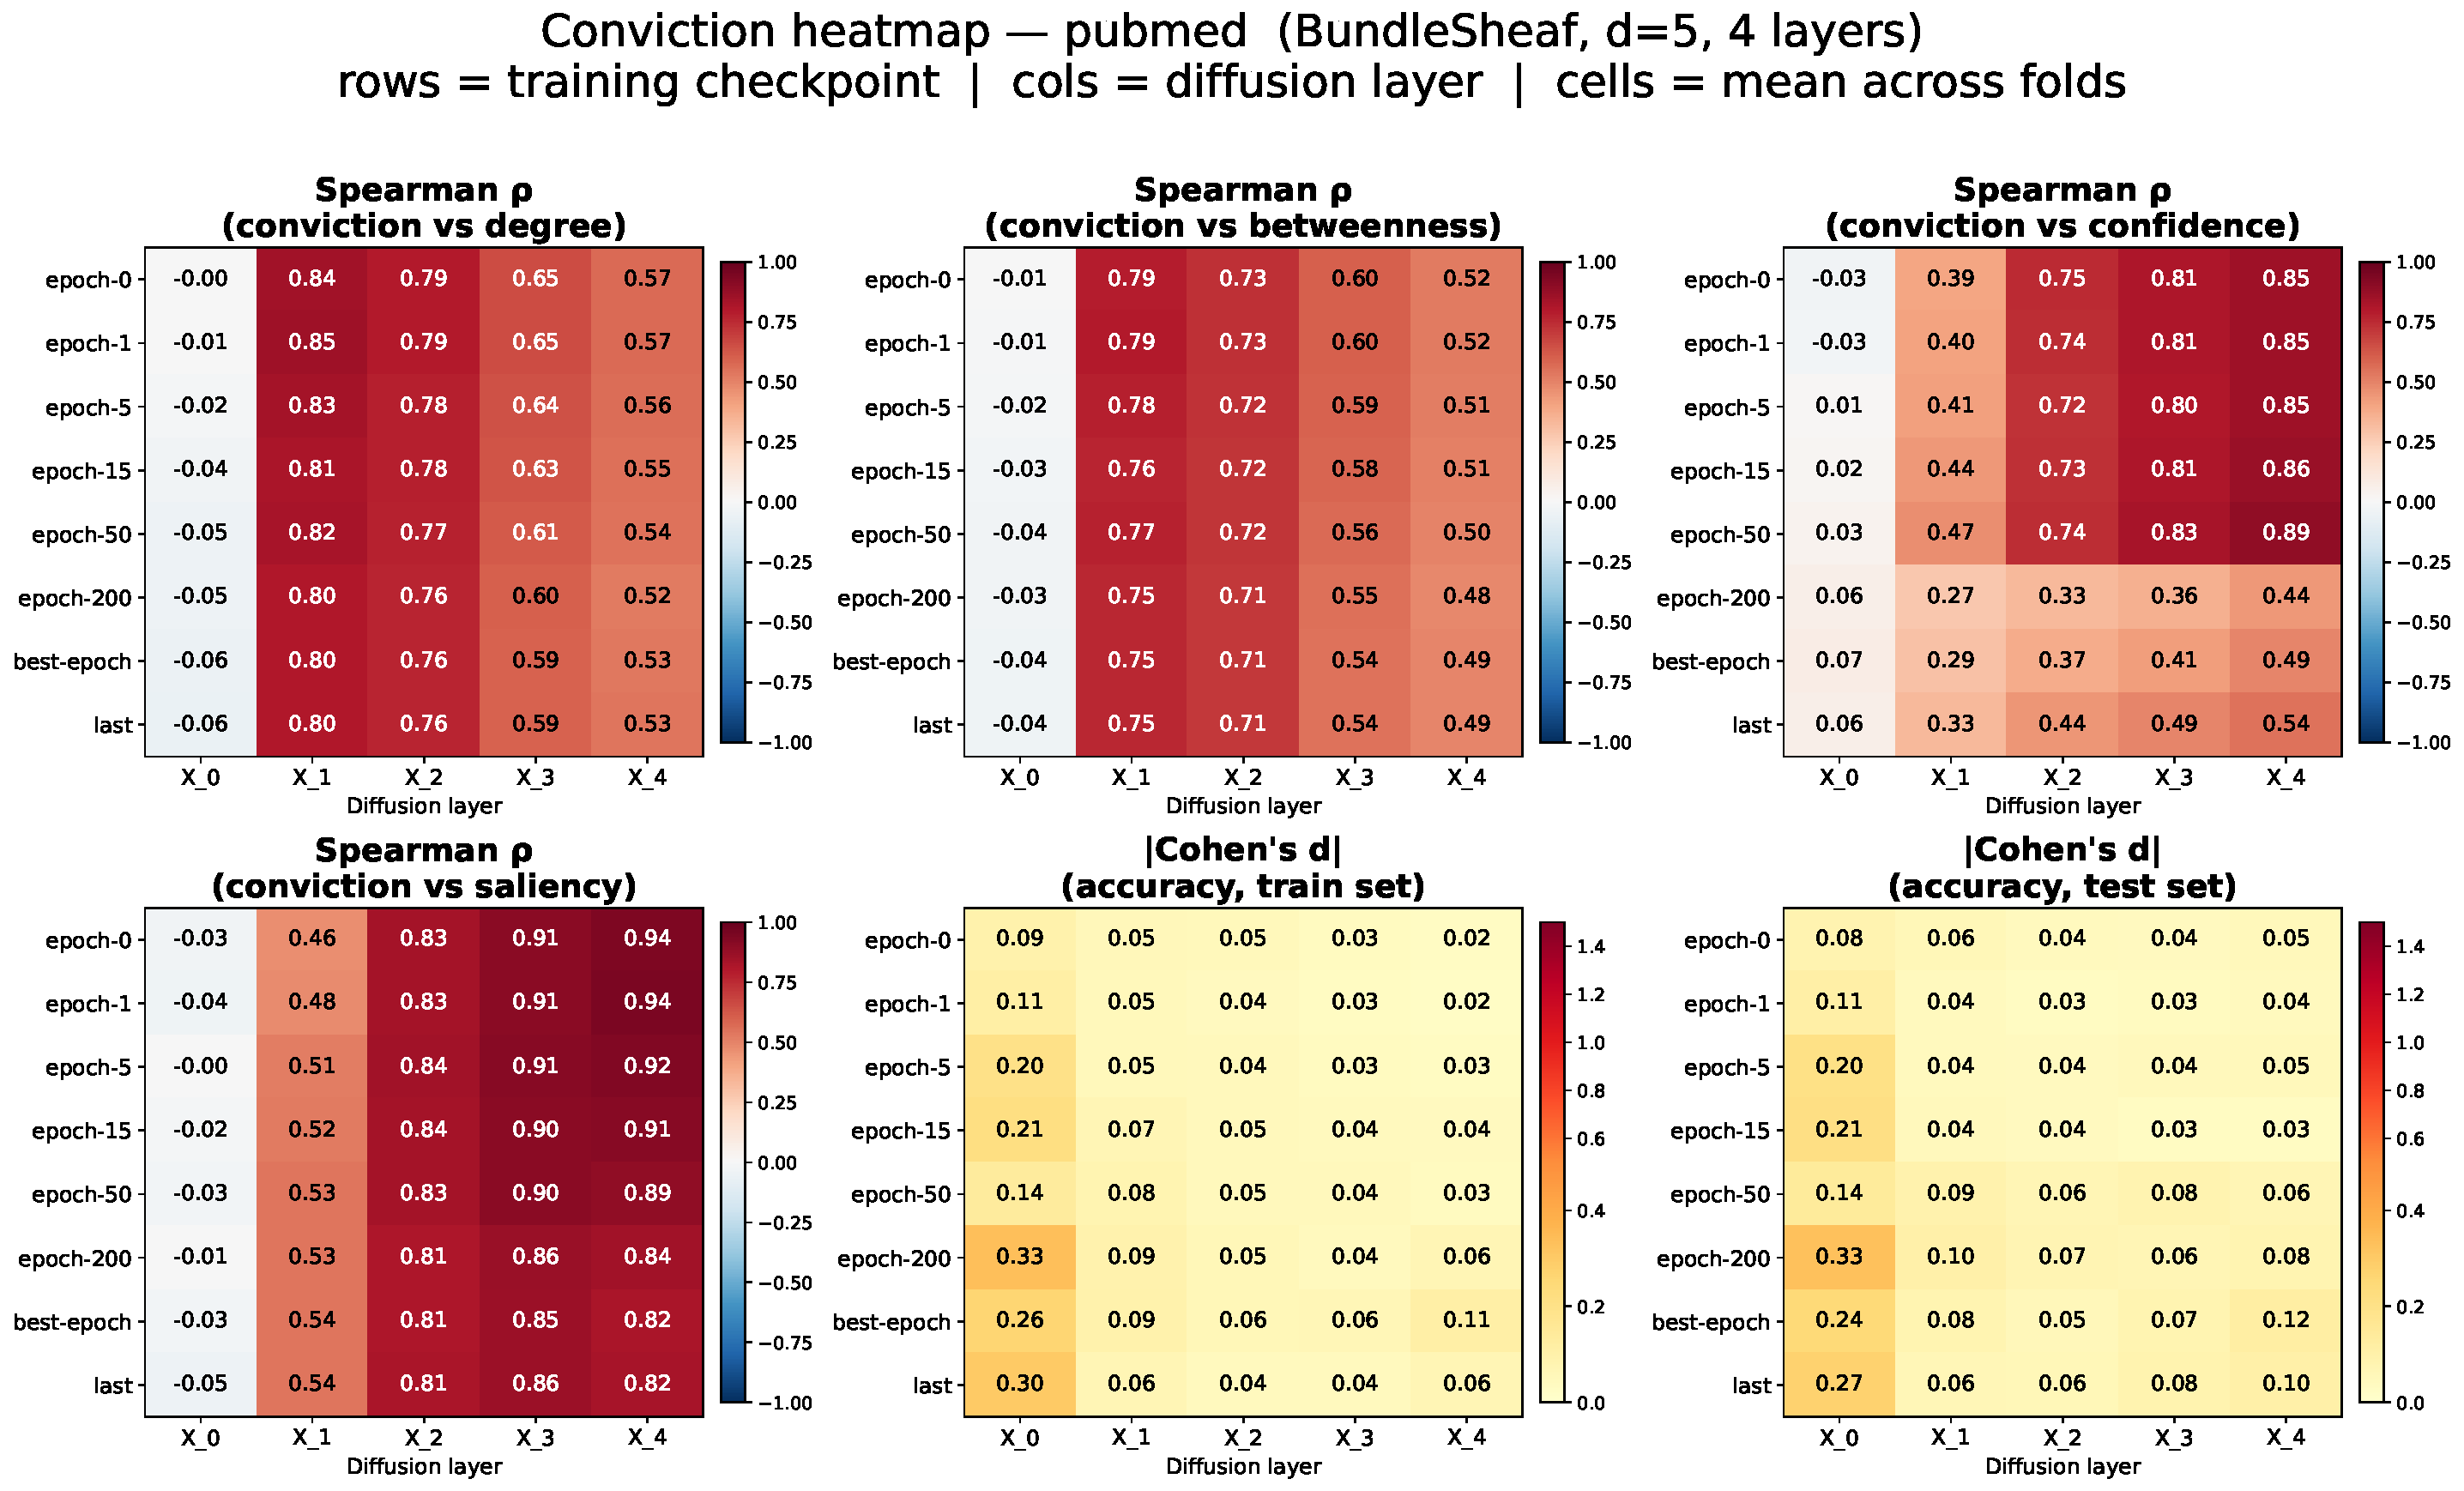
\includegraphics[width=\linewidth]{conviction_heatmap/BundleSheaf/normalised_false/pubmed_BundleSheaf_d5_4L_Norm_False_conviction_heatmap.pdf}
\end{figure}
\end{frame}

\begin{frame}{Questions --- BundleSheaf, $d=5$, $L=4$, Norm=False}
\begin{figure}
    \centering
    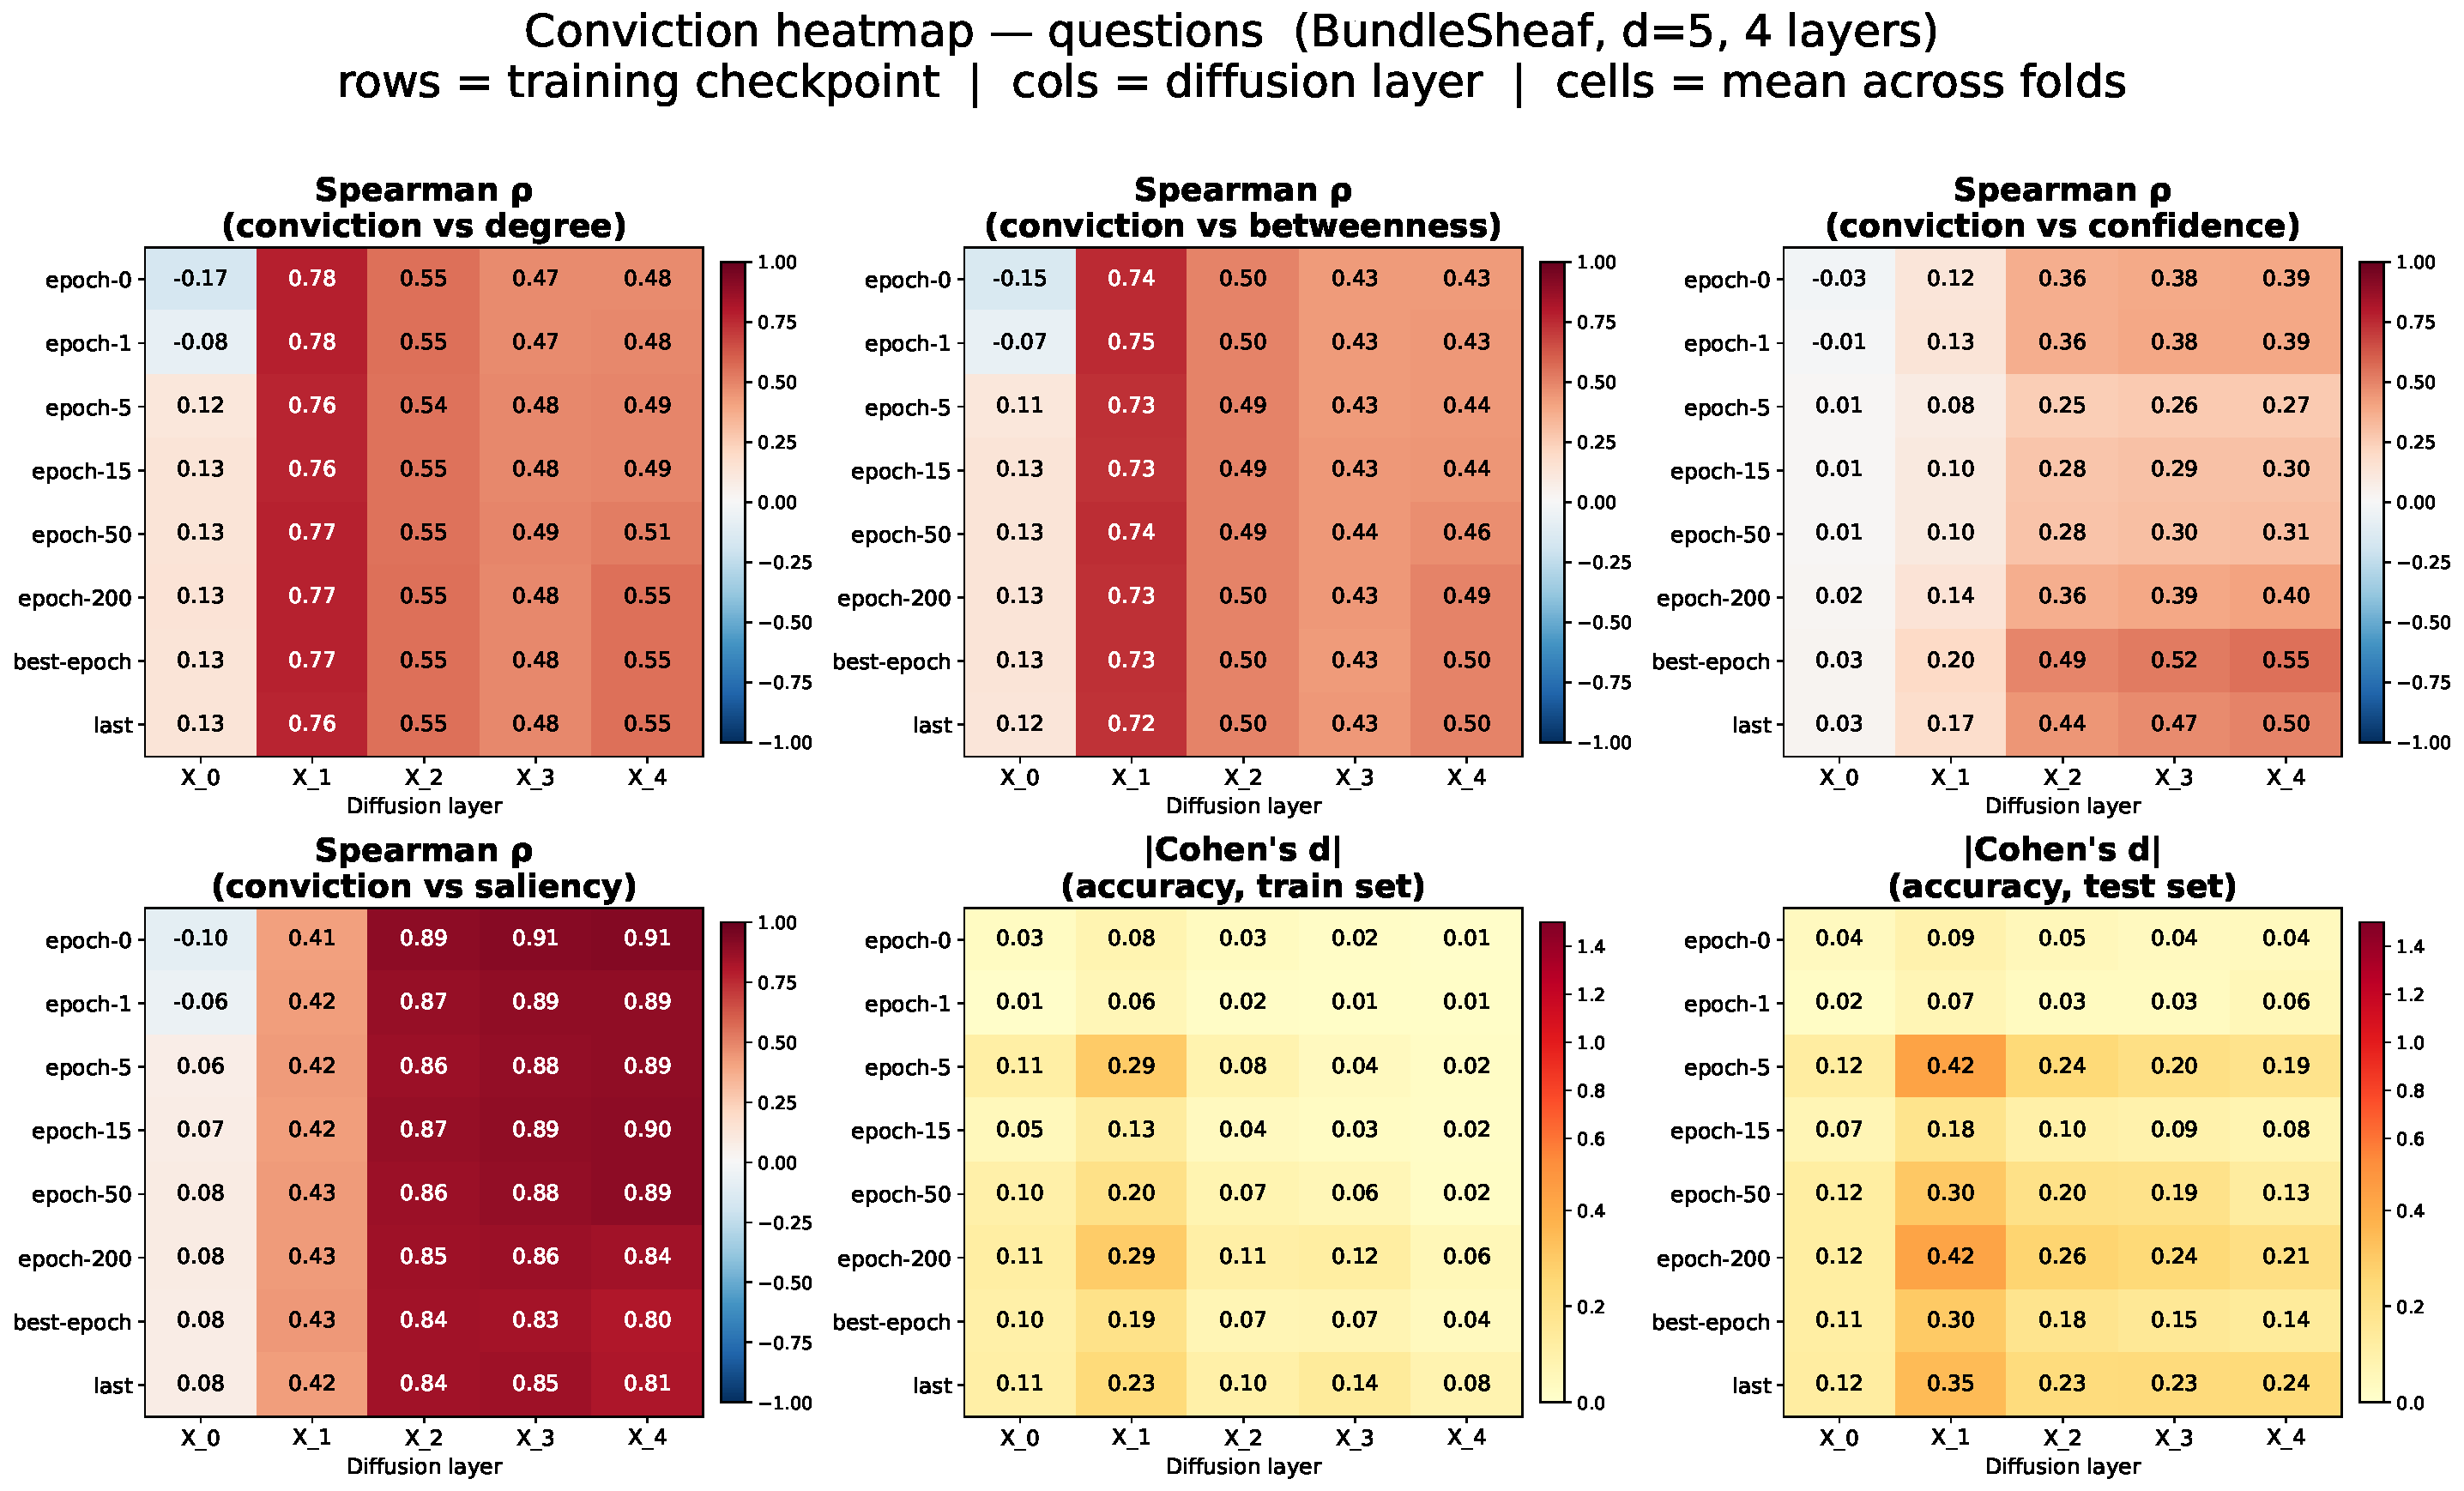
\includegraphics[width=\linewidth]{conviction_heatmap/BundleSheaf/normalised_false/questions_BundleSheaf_d5_4L_Norm_False_conviction_heatmap.pdf}
\end{figure}
\end{frame}

\begin{frame}{Roman Empire --- BundleSheaf, $d=5$, $L=5$, Norm=False}
\begin{figure}
    \centering
    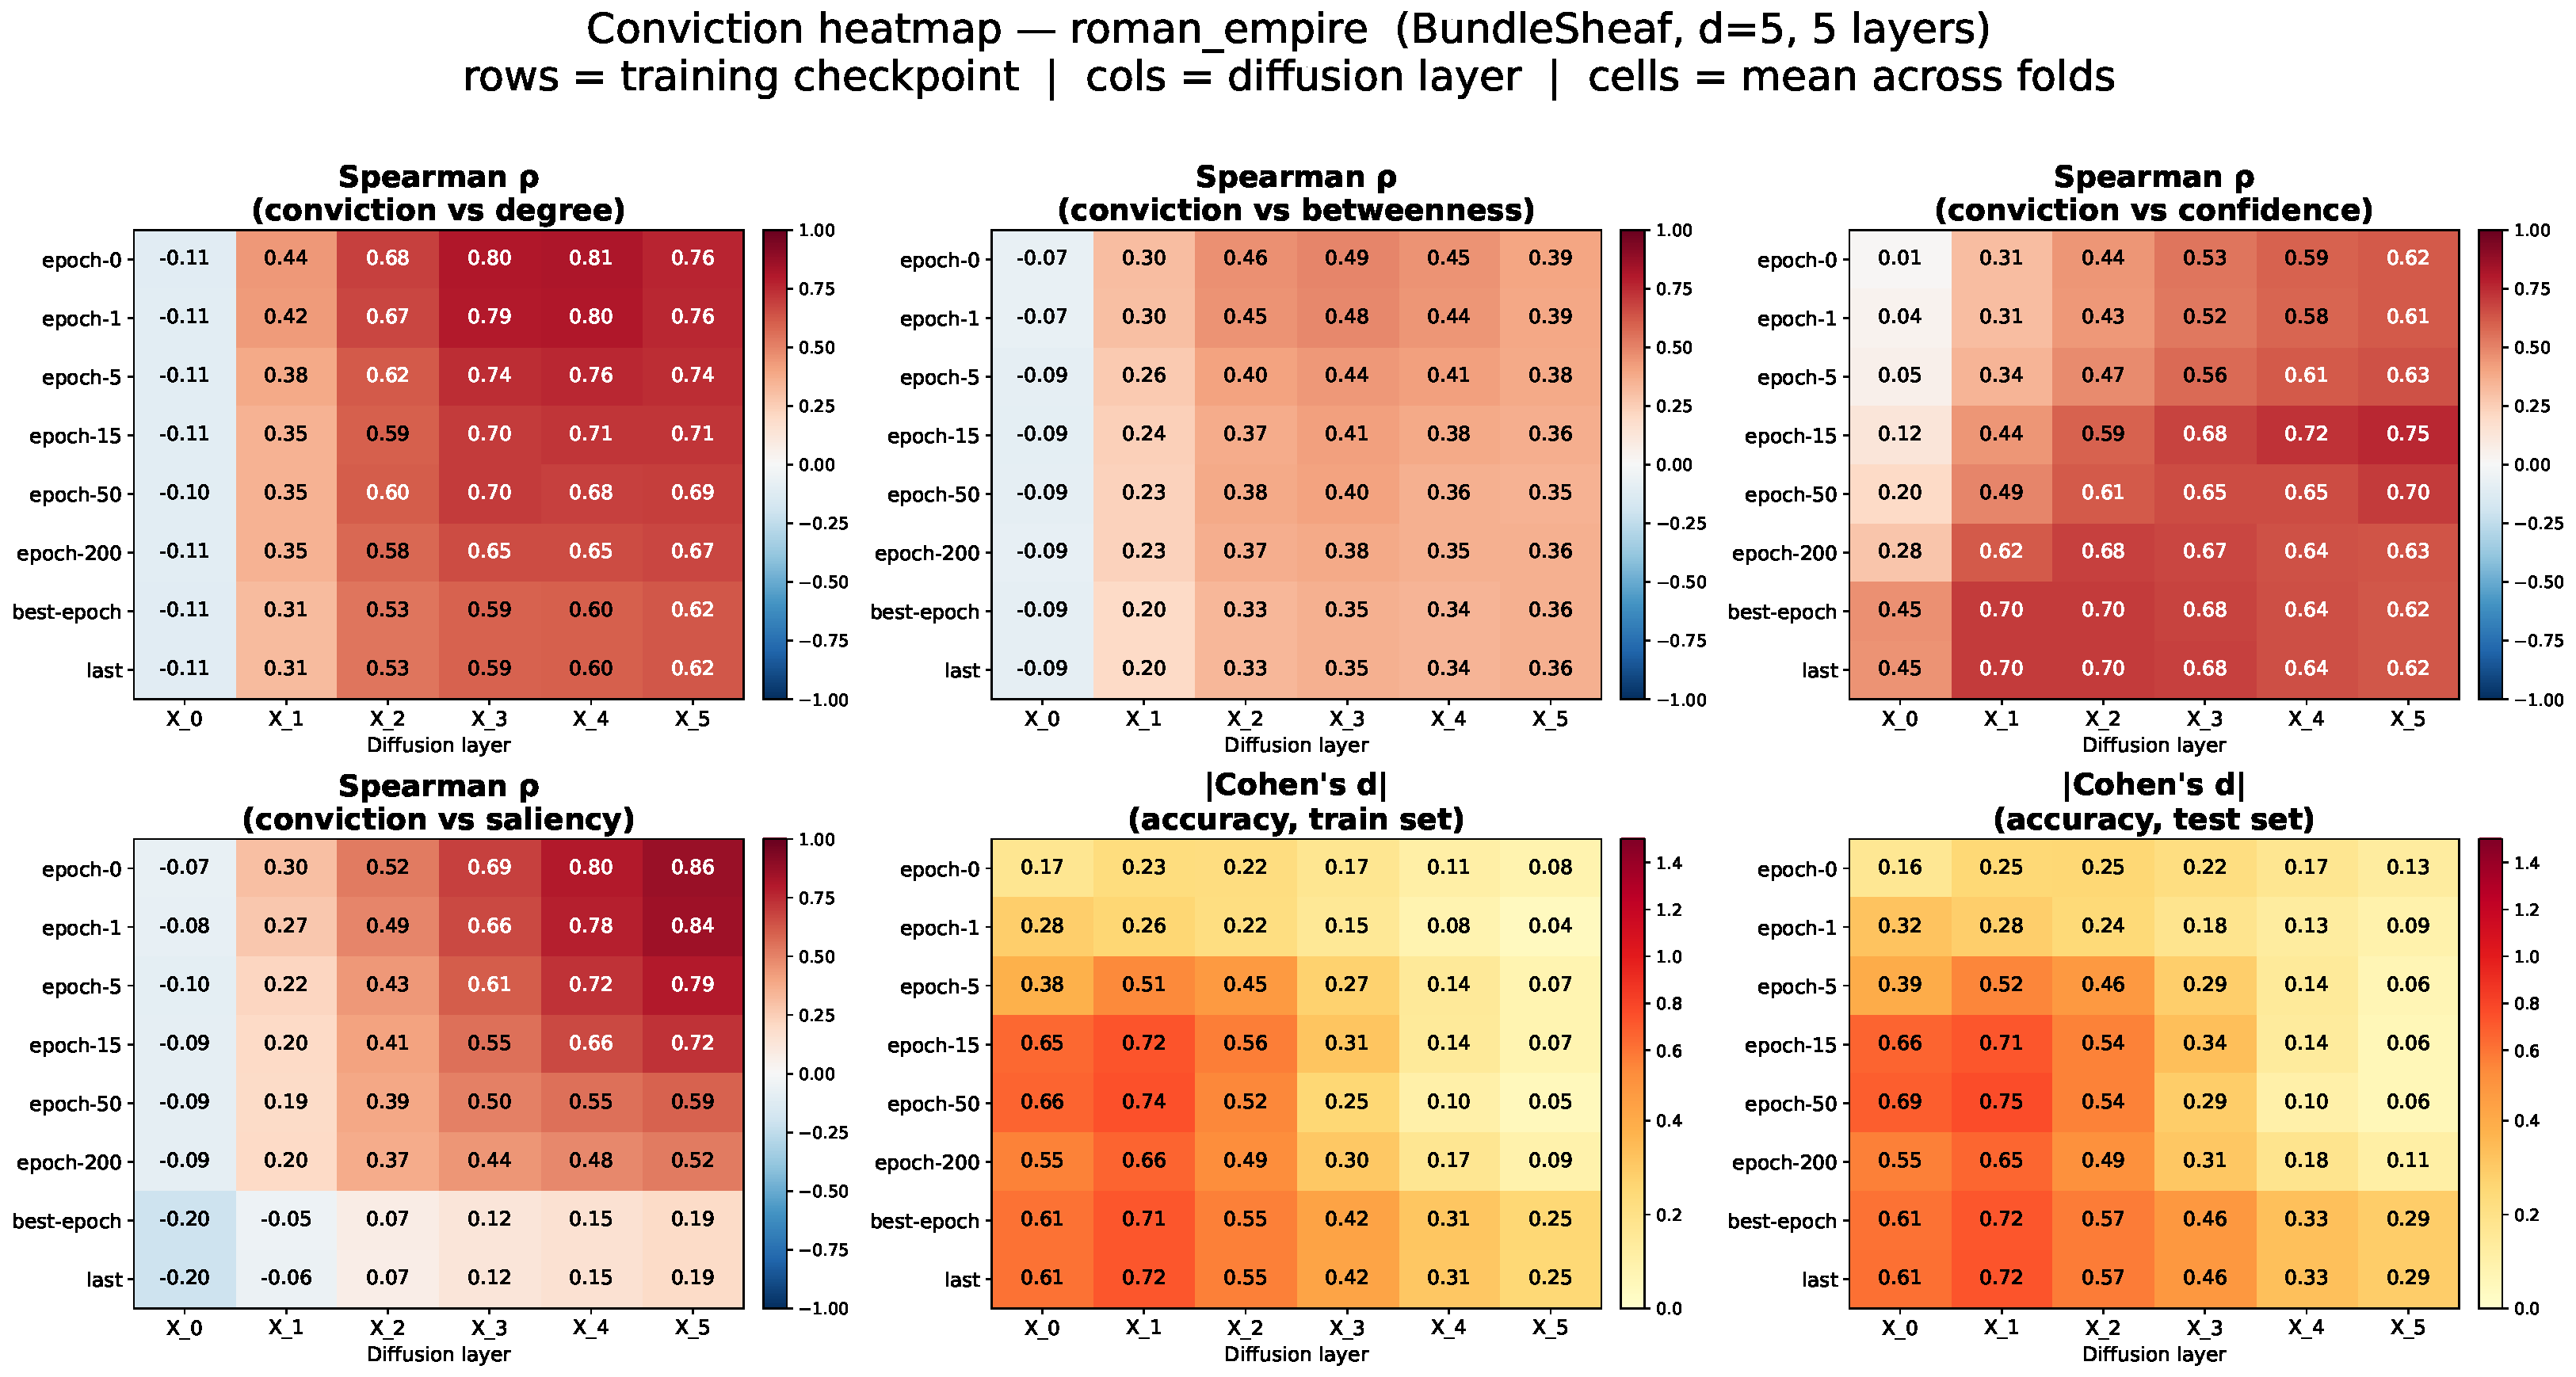
\includegraphics[width=\linewidth]{conviction_heatmap/BundleSheaf/normalised_false/roman_empire_BundleSheaf_d5_5L_Norm_False_conviction_heatmap.pdf}
\end{figure}
\end{frame}

\begin{frame}{Tolokers --- BundleSheaf, $d=3$, $L=4$, Norm=False}
\begin{figure}
    \centering
    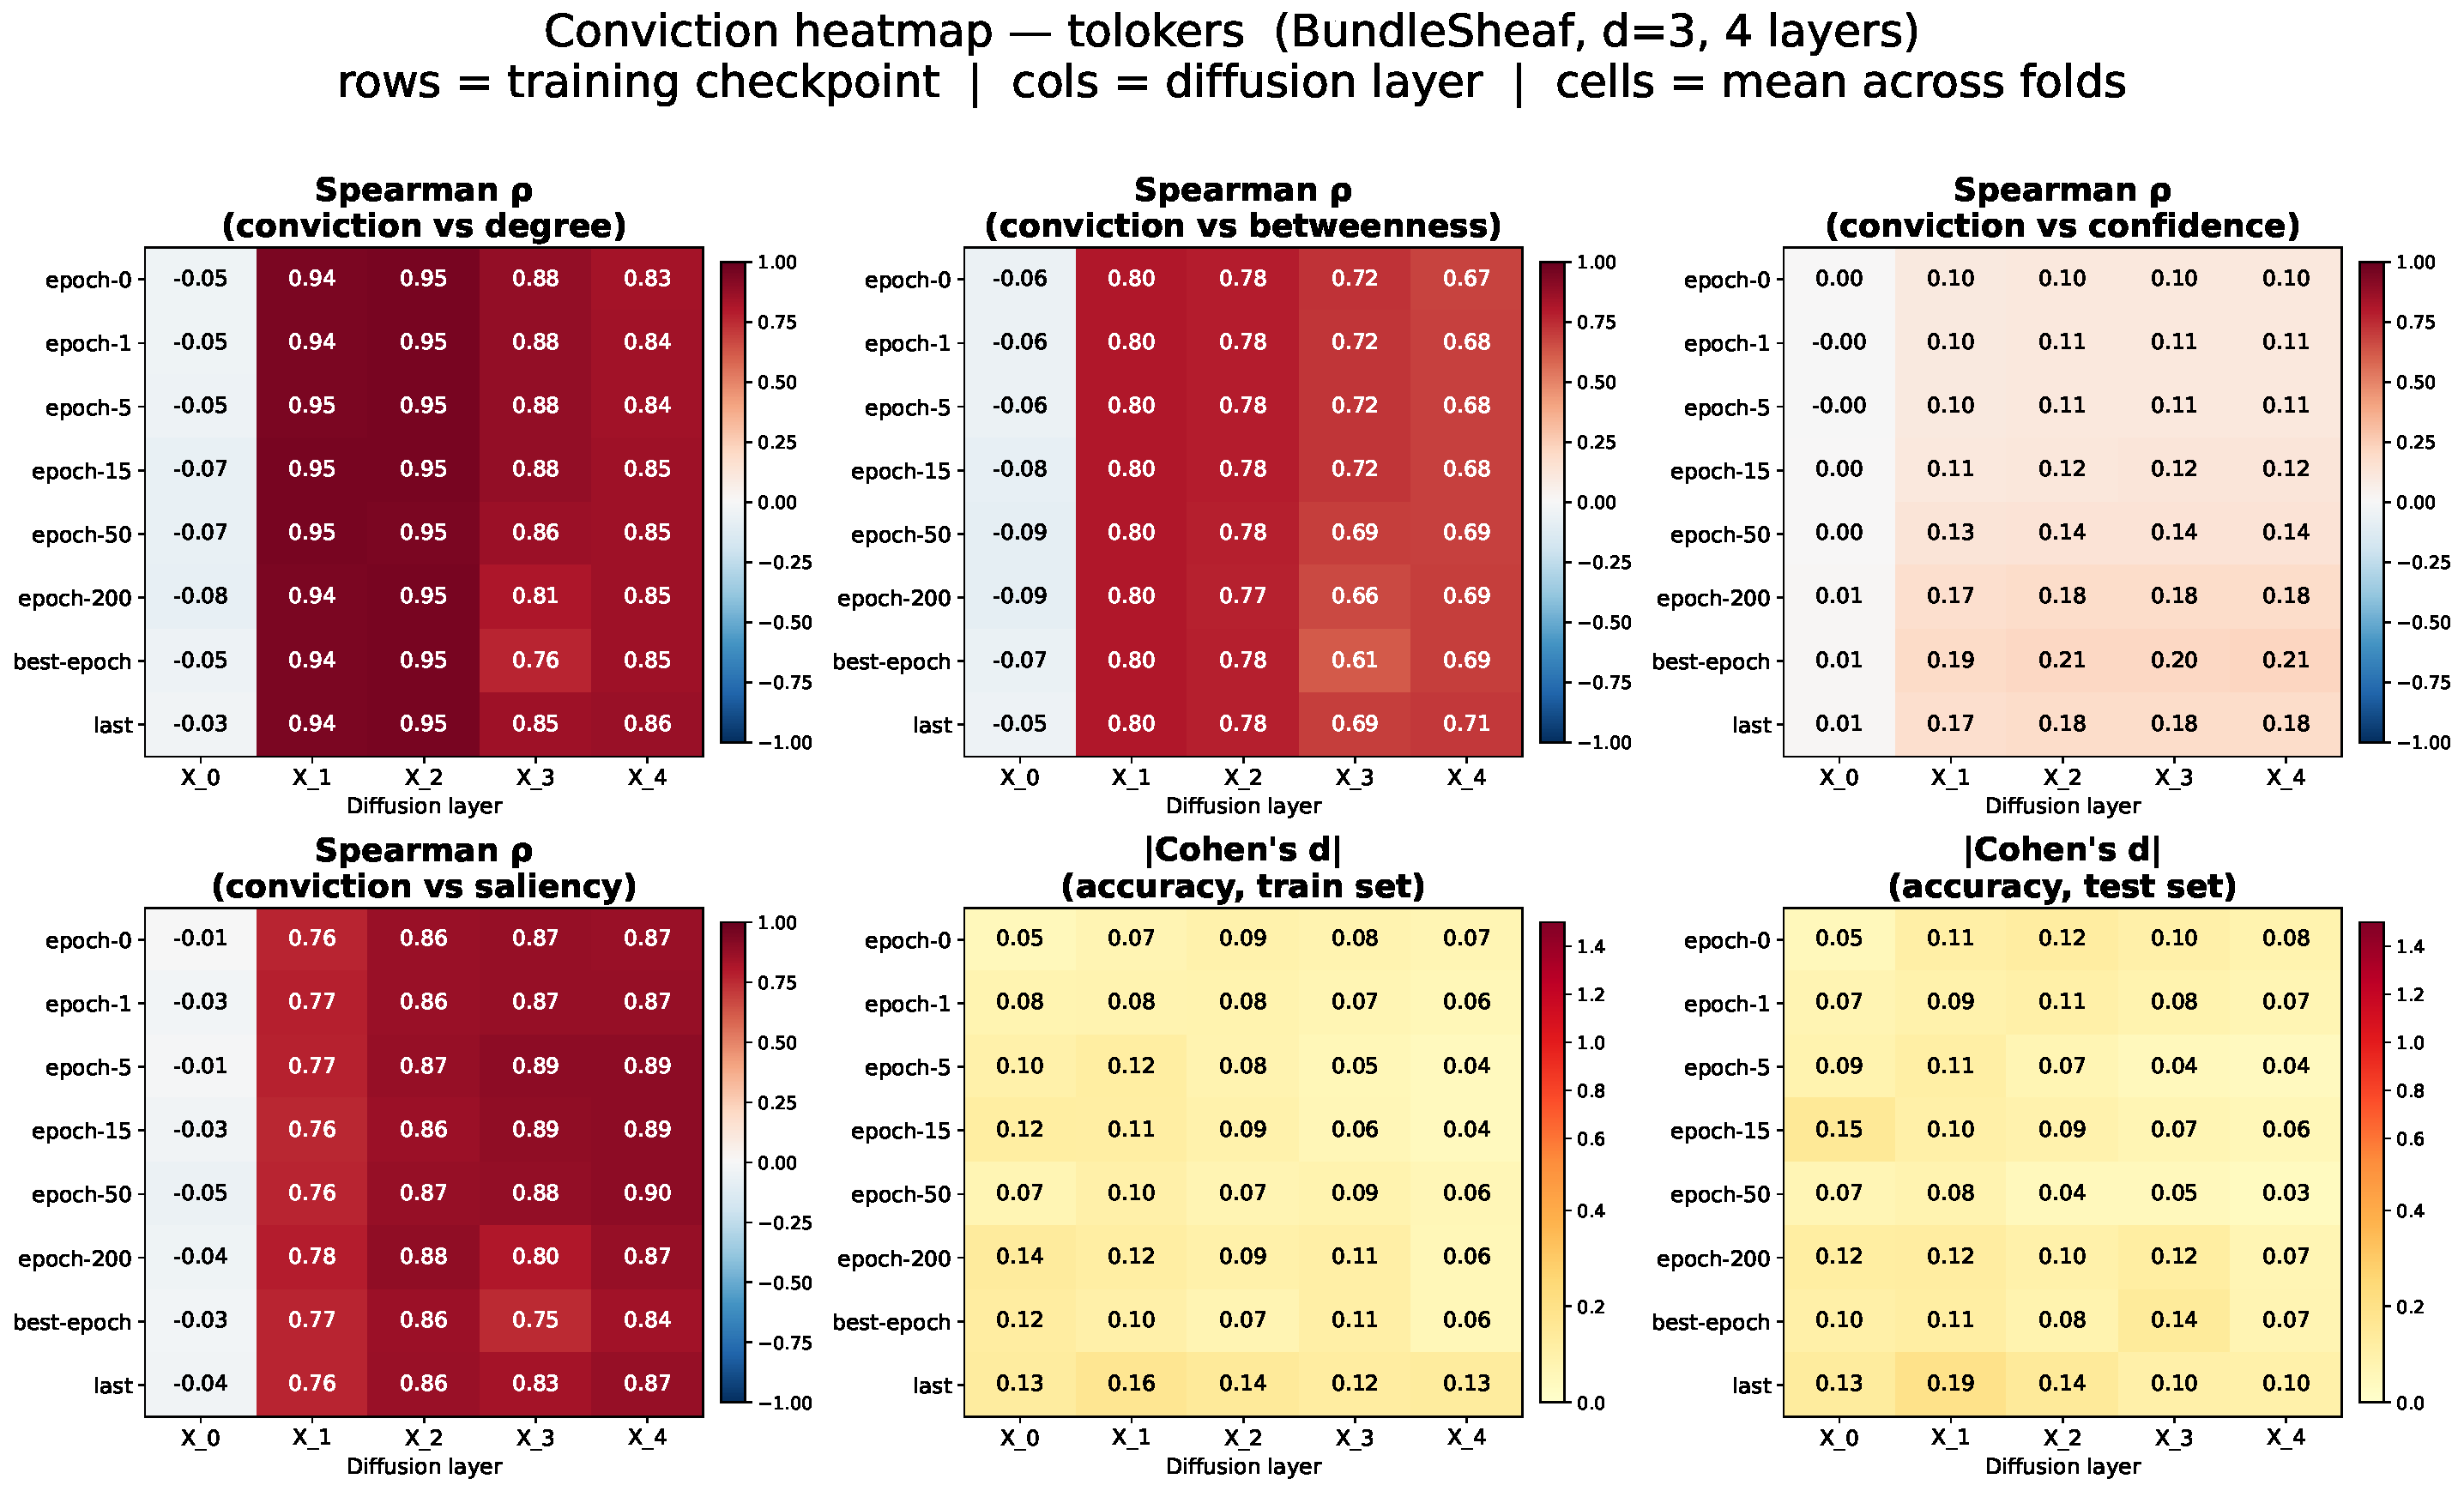
\includegraphics[width=\linewidth]{conviction_heatmap/BundleSheaf/normalised_false/tolokers_BundleSheaf_d3_4L_Norm_False_conviction_heatmap.pdf}
\end{figure}
\end{frame}

\begin{frame}{Wisconsin --- BundleSheaf, $d=2$, $L=2$, Norm=False}
\begin{figure}
    \centering
    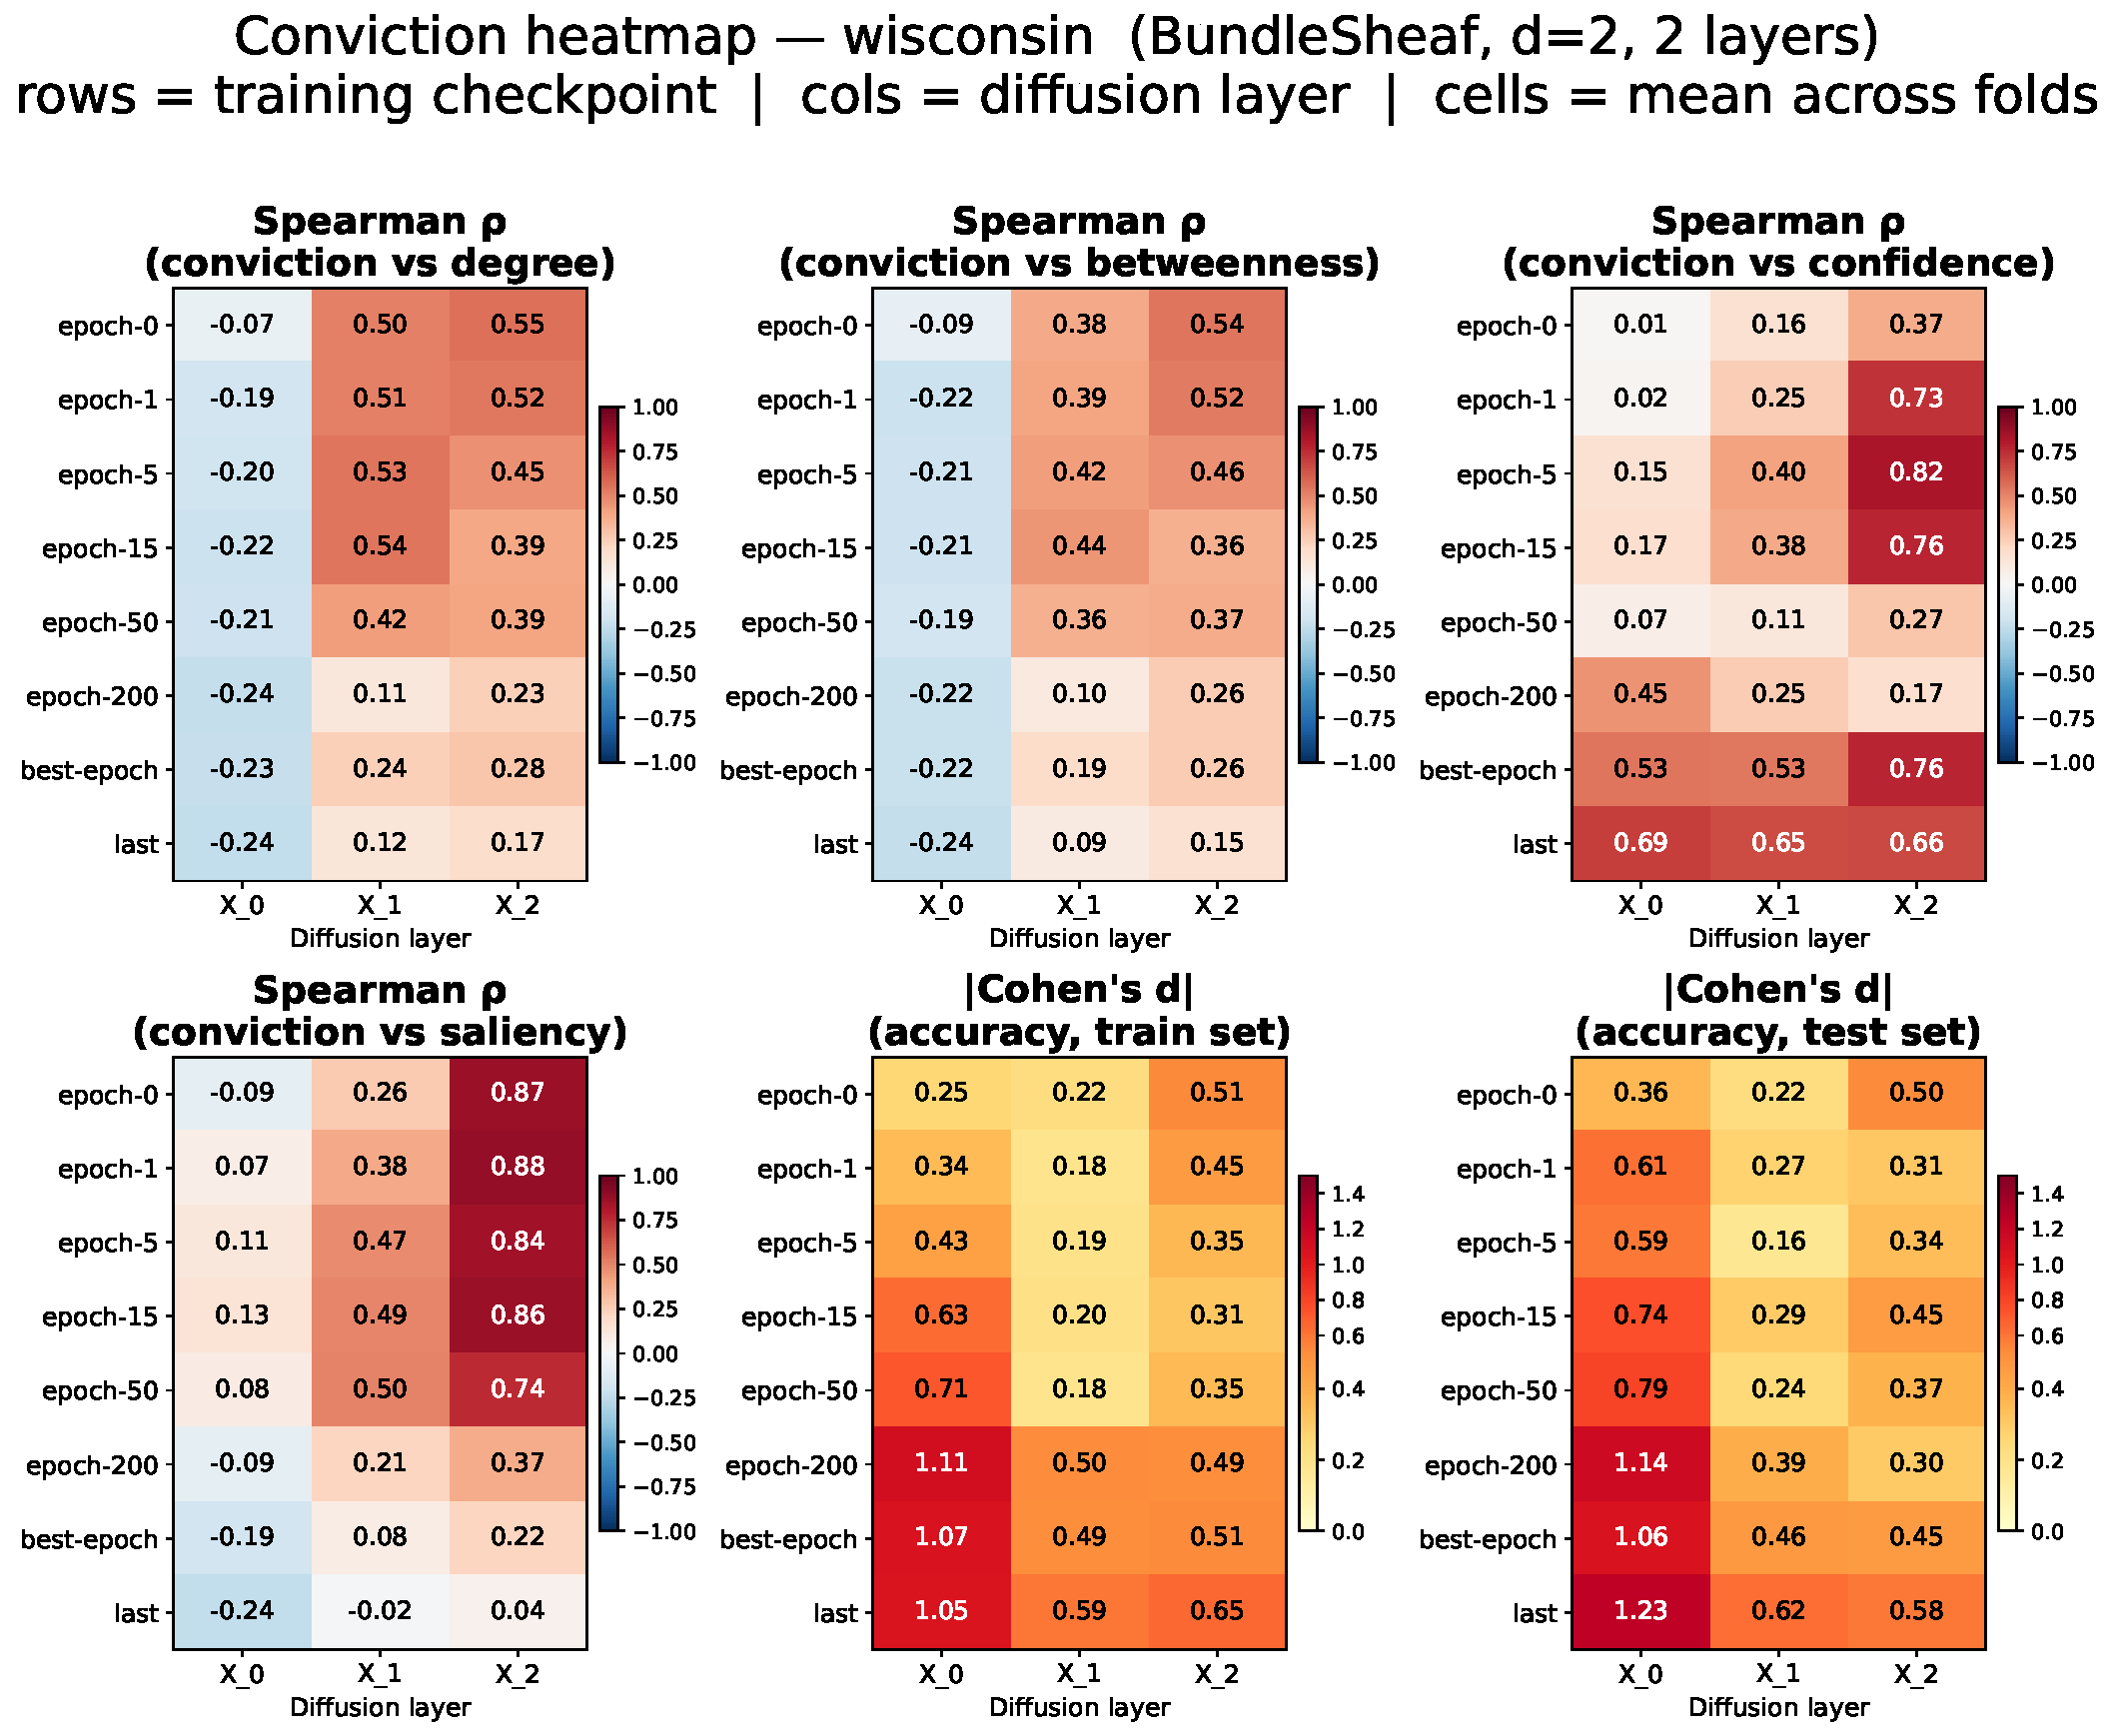
\includegraphics[width=0.8\linewidth]{conviction_heatmap/BundleSheaf/normalised_false/wisconsin_BundleSheaf_d2_2L_Norm_False_conviction_heatmap.pdf}
\end{figure}
\end{frame}




% ══════════════════════════════════════════════════════════════════════════════
%  SECTION 6 — Scatter, BundleSheaf, normalised=False
% ══════════════════════════════════════════════════════════════════════════════

\begin{frame}{}
\centering
\Huge\textbf{Conviction Scatter}\\[6pt]
\Large BundleSheaf \quad (\texttt{normalised=False})
\end{frame}

\begin{frame}{Amazon Ratings --- BundleSheaf, $d=5$, $L=5$, Norm=False}
\begin{figure}
    \centering
    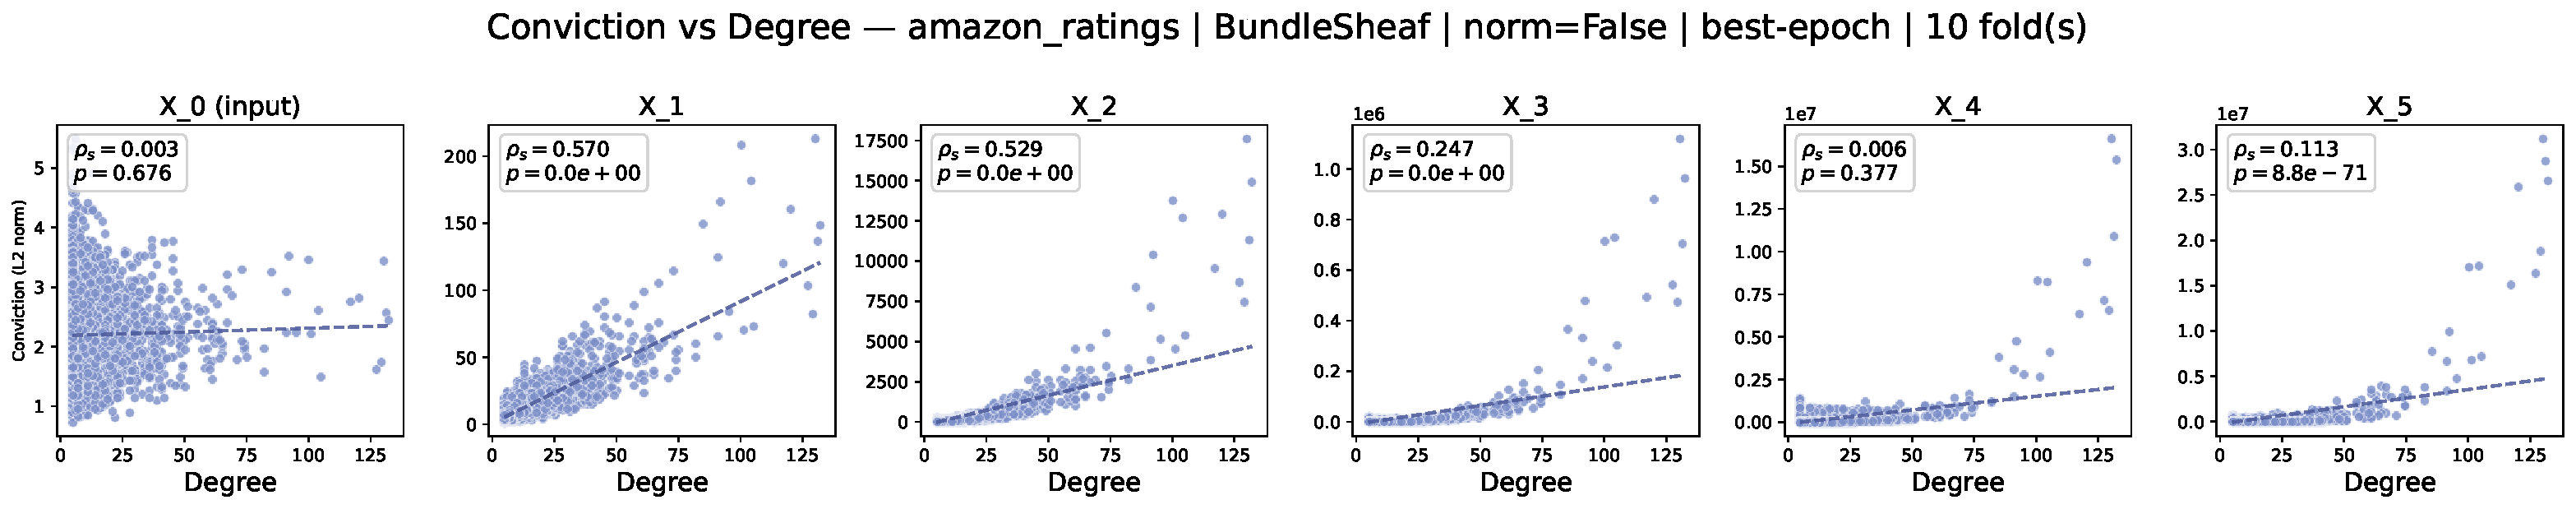
\includegraphics[width=\linewidth]{conviction_scatter/BundleSheaf/normalised_false/amazon_ratings_BundleSheaf_d5_5L_Norm_False_conviction_scatter.pdf}
\end{figure}
\end{frame}

\begin{frame}{Citeseer --- BundleSheaf, $d=5$, $L=4$, Norm=False}
\begin{figure}
    \centering
    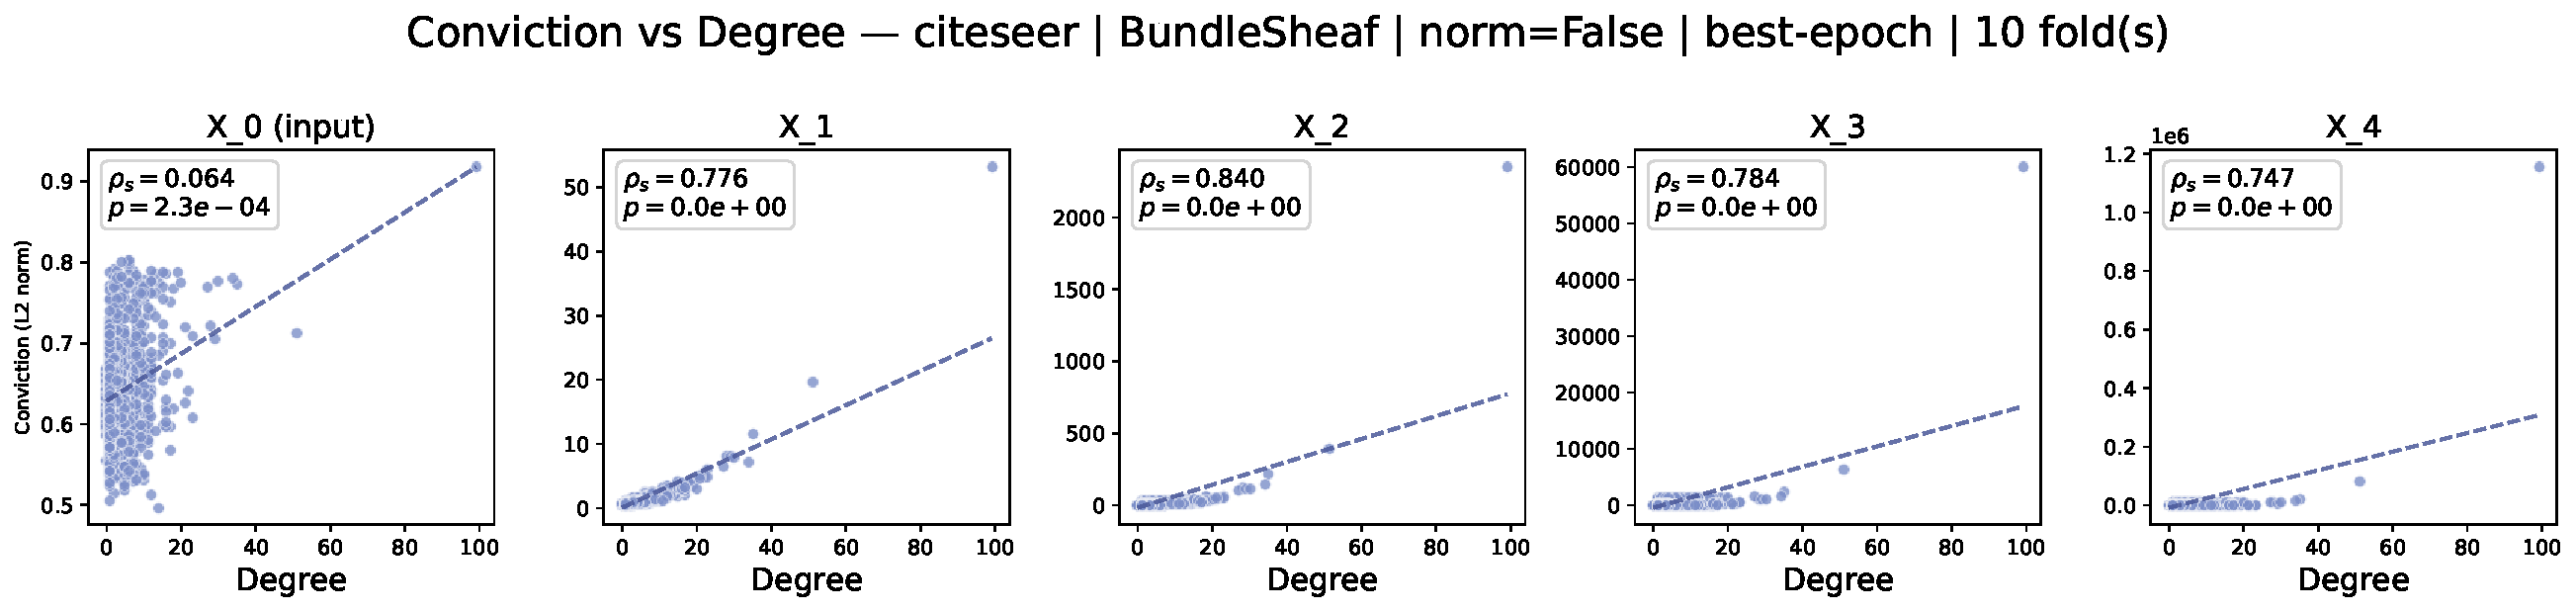
\includegraphics[width=\linewidth]{conviction_scatter/BundleSheaf/normalised_false/citeseer_BundleSheaf_d5_4L_Norm_False_conviction_scatter.pdf}
\end{figure}
\end{frame}

\begin{frame}{Cora --- BundleSheaf, $d=5$, $L=3$, Norm=False}
\begin{figure}
    \centering
    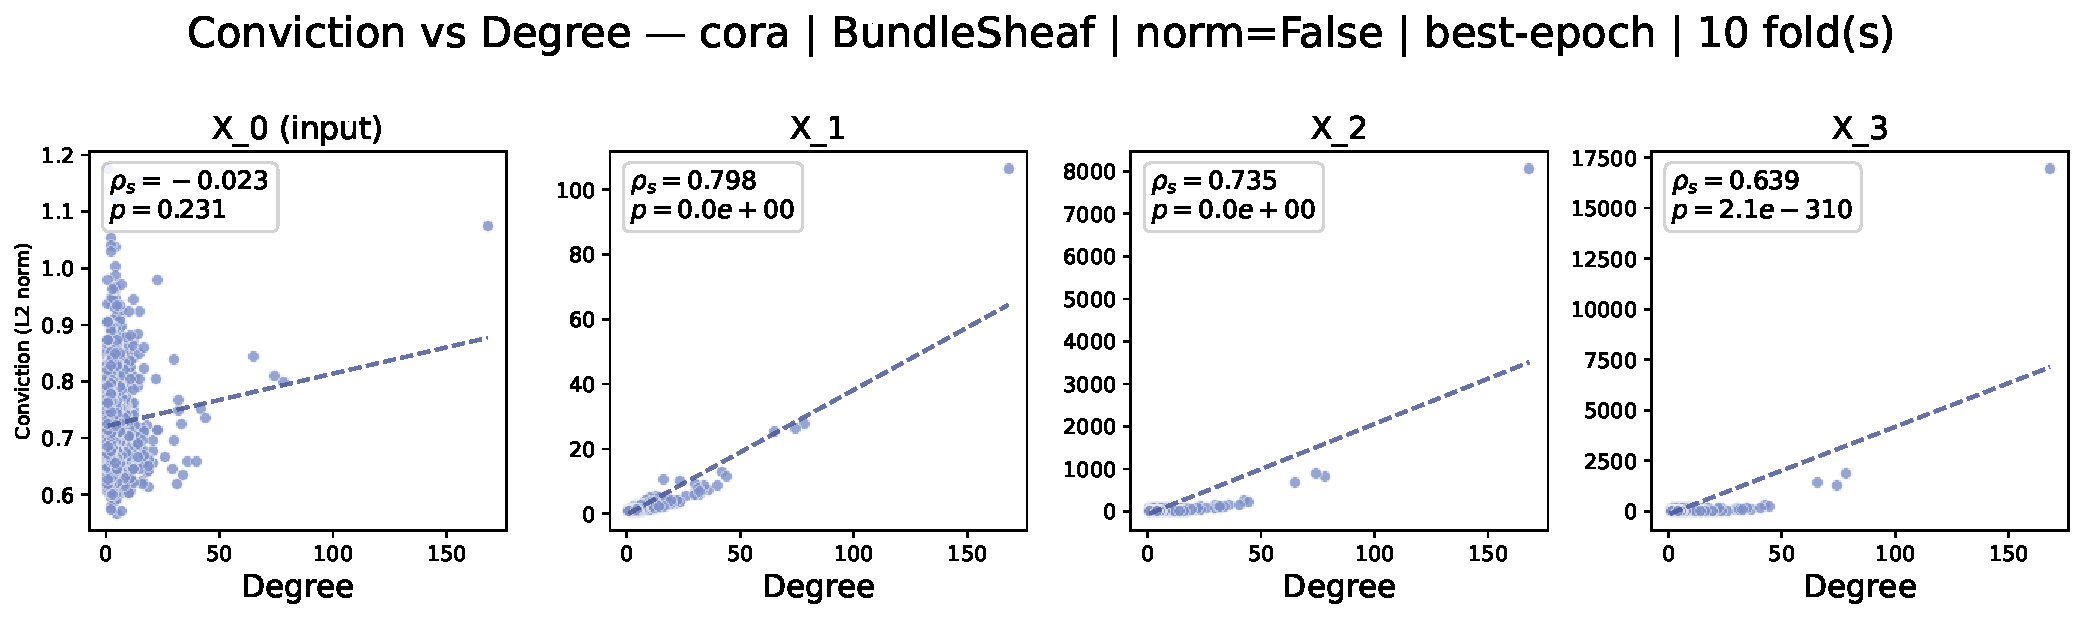
\includegraphics[width=\linewidth]{conviction_scatter/BundleSheaf/normalised_false/cora_BundleSheaf_d5_3L_Norm_False_conviction_scatter.pdf}
\end{figure}
\end{frame}

\begin{frame}{Cornell --- BundleSheaf, $d=2$, $L=2$, Norm=False}
\begin{figure}
    \centering
    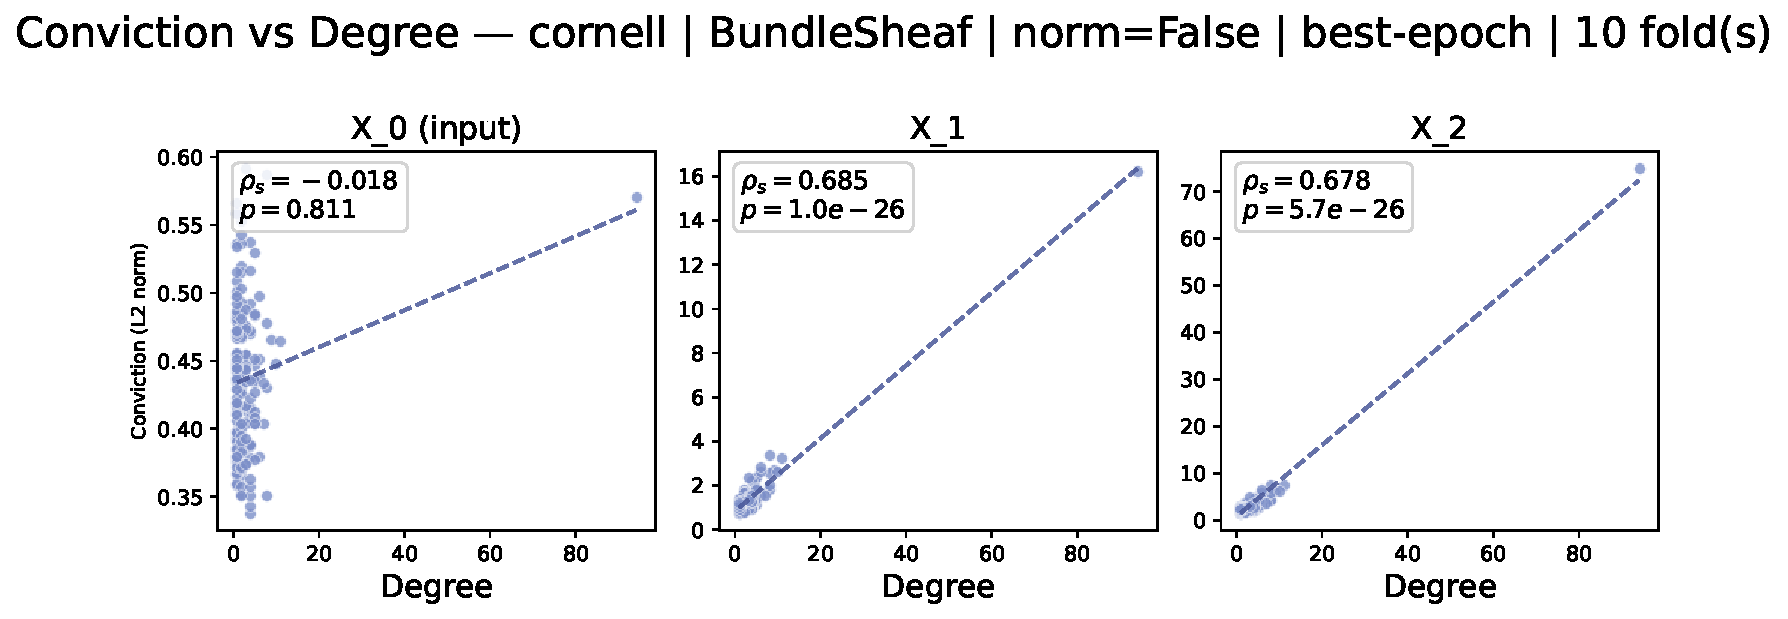
\includegraphics[width=0.8\linewidth]{conviction_scatter/BundleSheaf/normalised_false/cornell_BundleSheaf_d2_2L_Norm_False_conviction_scatter.pdf}
\end{figure}
\end{frame}

\begin{frame}{Minesweeper --- BundleSheaf, $d=5$, $L=6$, Norm=False}
\begin{figure}
    \centering
    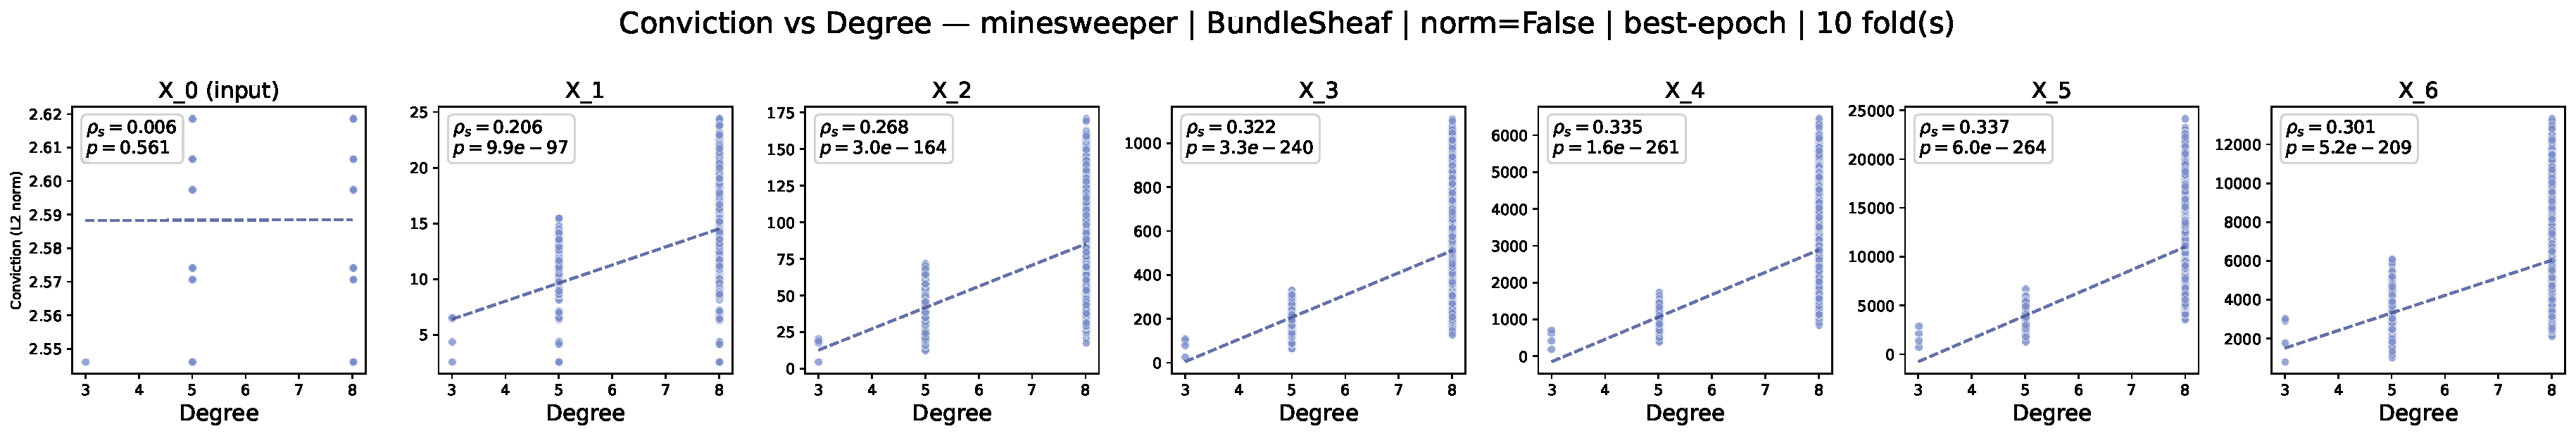
\includegraphics[width=\linewidth]{conviction_scatter/BundleSheaf/normalised_false/minesweeper_BundleSheaf_d5_6L_Norm_False_conviction_scatter.pdf}
\end{figure}
\end{frame}

\begin{frame}{Pubmed --- BundleSheaf, $d=5$, $L=4$, Norm=False}
\begin{figure}
    \centering
    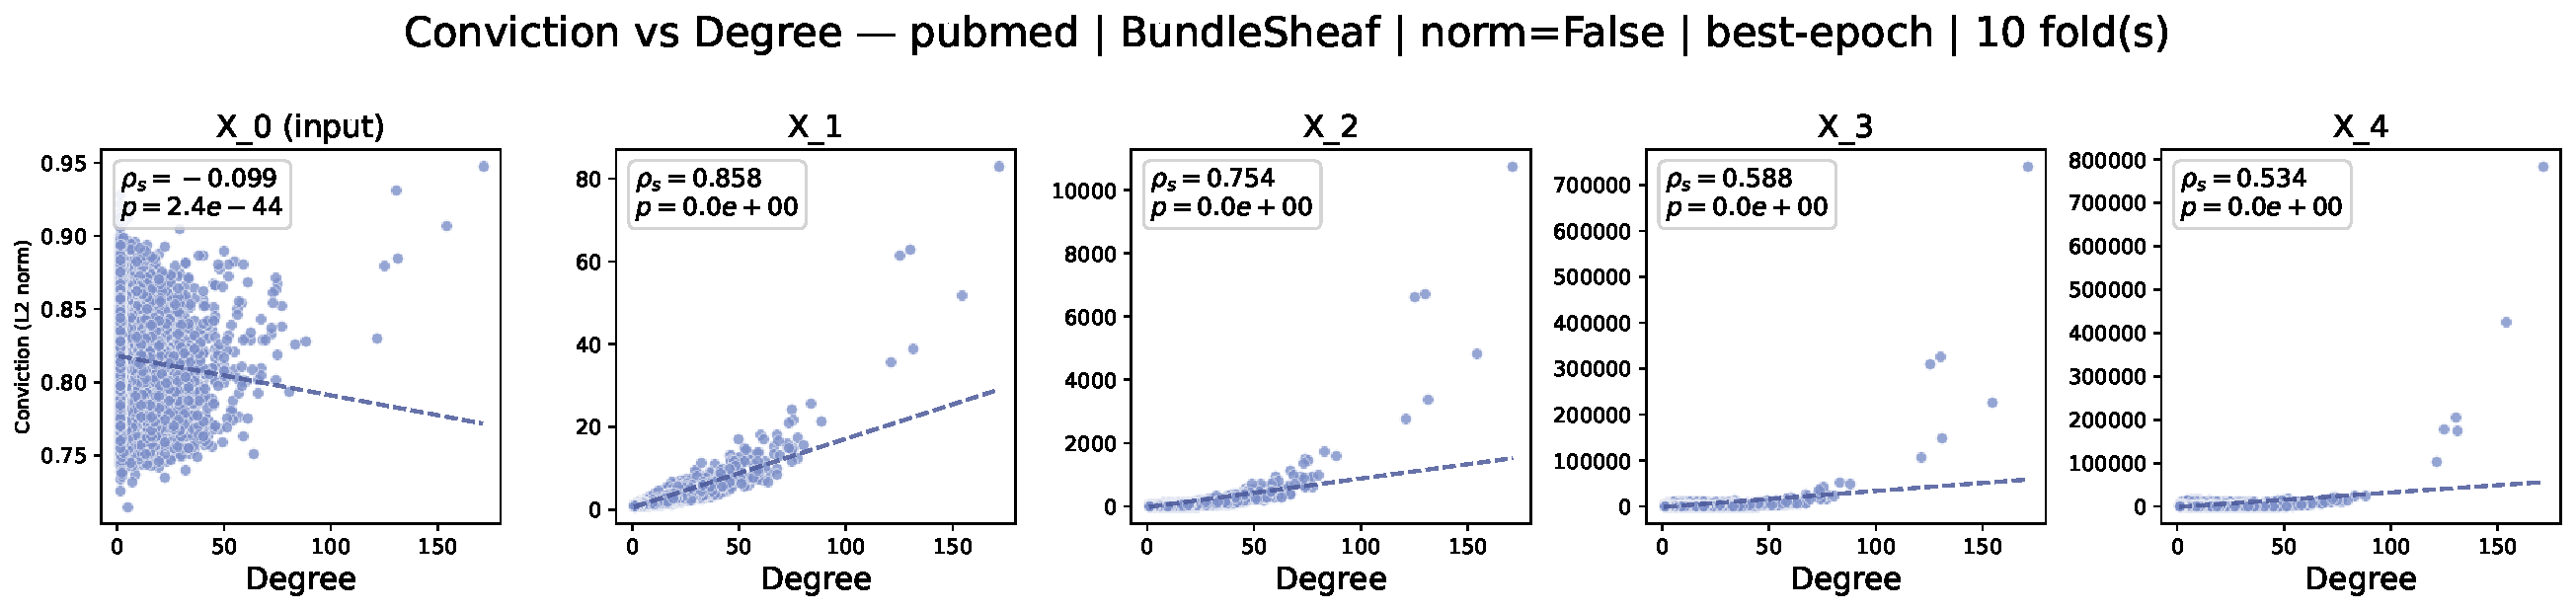
\includegraphics[width=\linewidth]{conviction_scatter/BundleSheaf/normalised_false/pubmed_BundleSheaf_d5_4L_Norm_False_conviction_scatter.pdf}
\end{figure}
\end{frame}

\begin{frame}{Questions --- BundleSheaf, $d=5$, $L=4$, Norm=False}
\begin{figure}
    \centering
    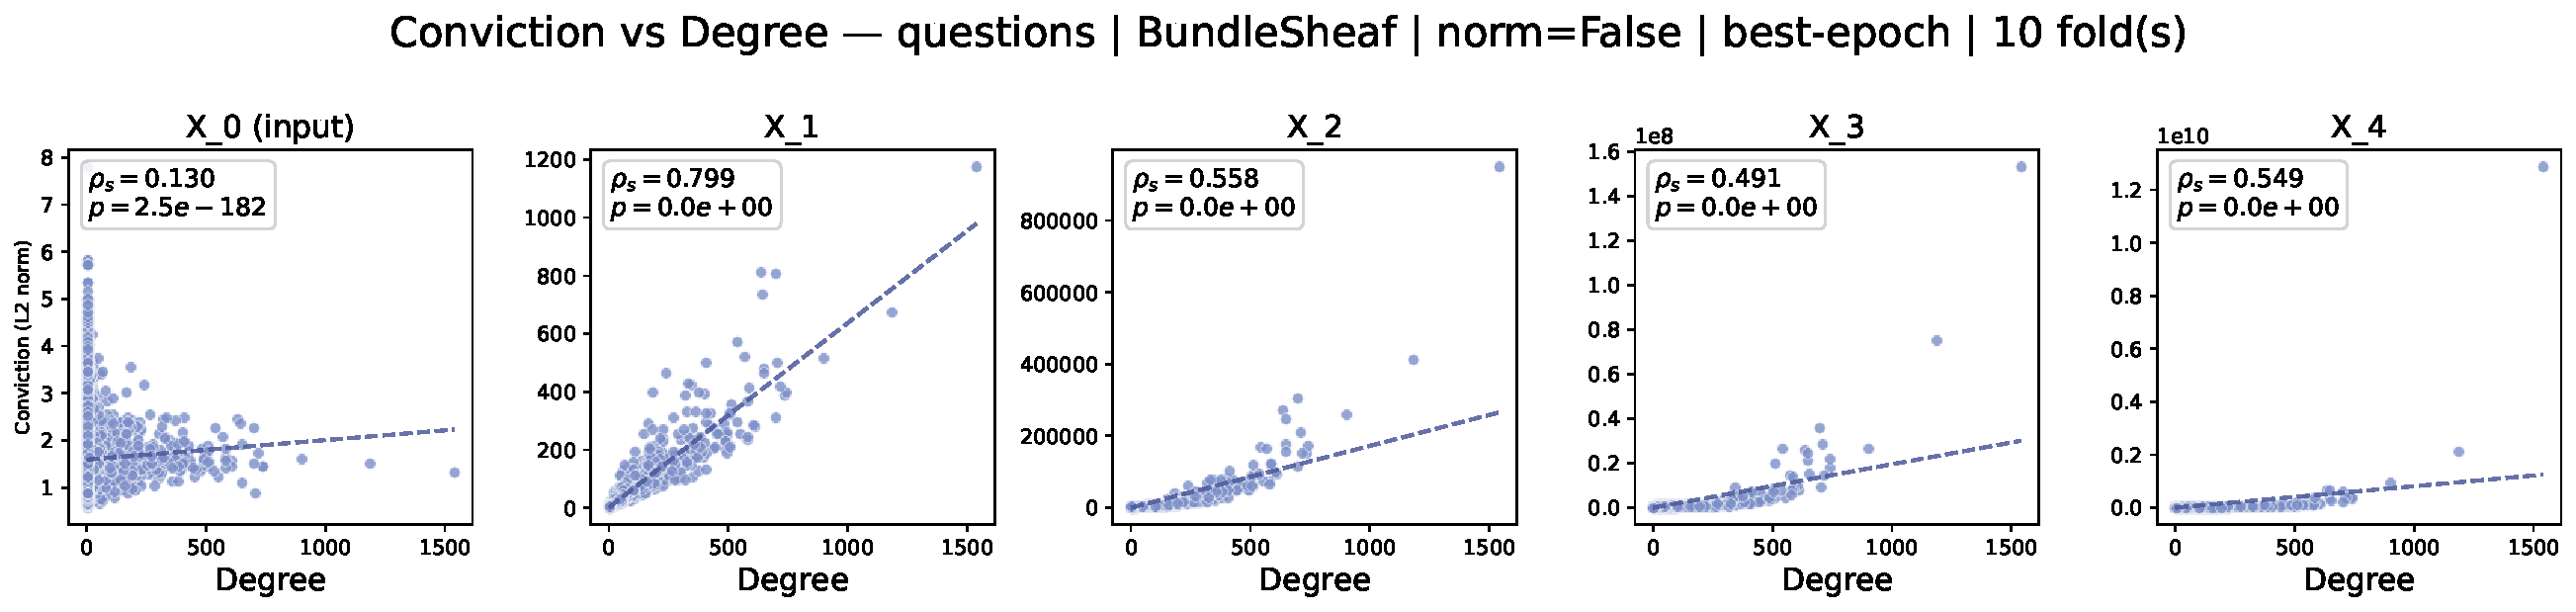
\includegraphics[width=\linewidth]{conviction_scatter/BundleSheaf/normalised_false/questions_BundleSheaf_d5_4L_Norm_False_conviction_scatter.pdf}
\end{figure}
\end{frame}

\begin{frame}{Roman Empire --- BundleSheaf, $d=5$, $L=5$, Norm=False}
\begin{figure}
    \centering
    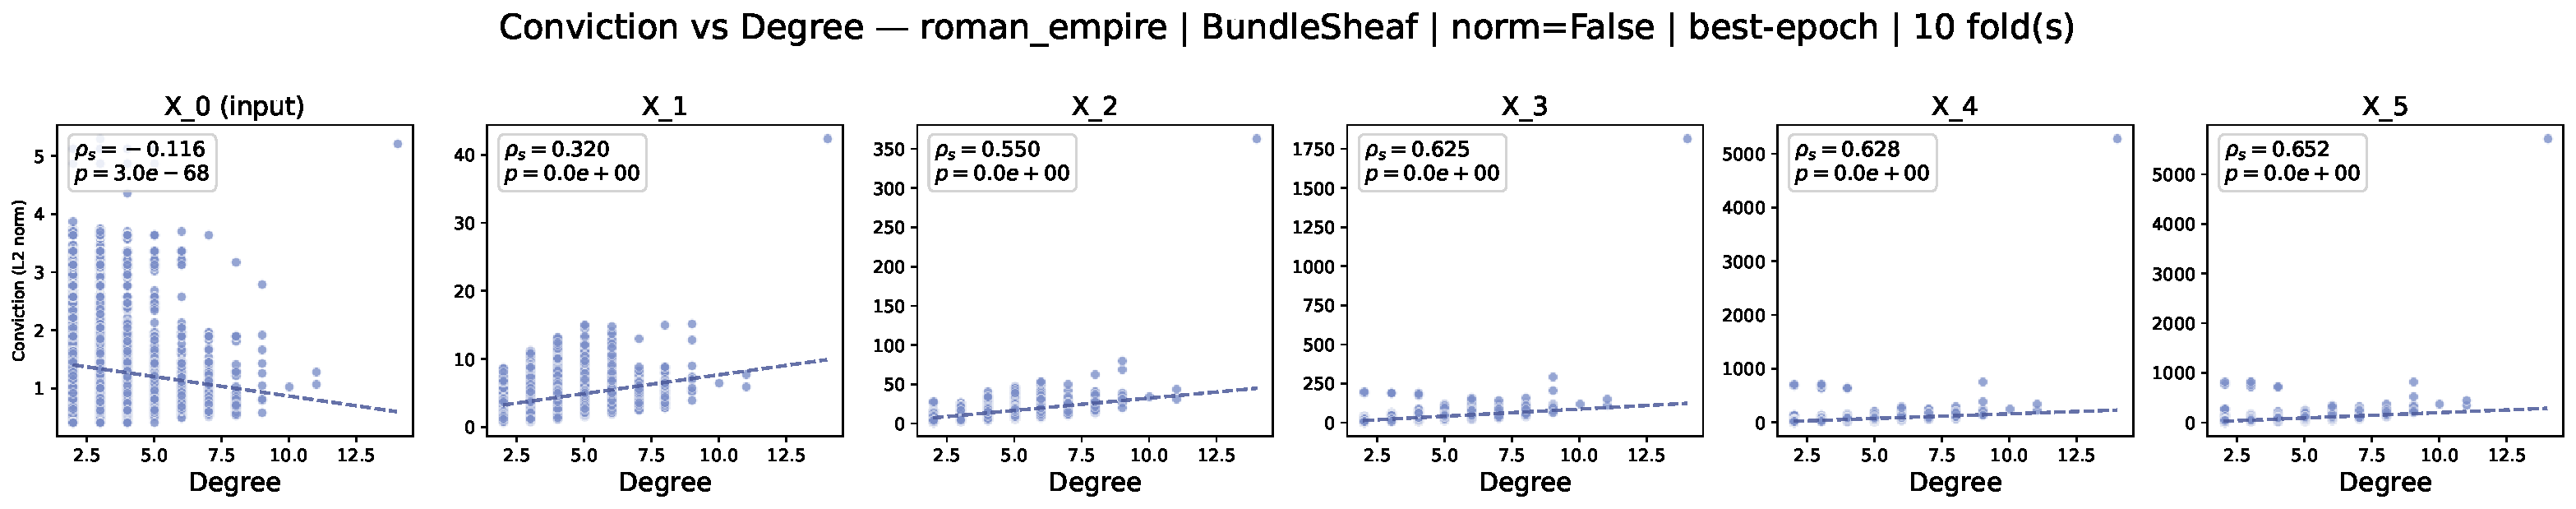
\includegraphics[width=\linewidth]{conviction_scatter/BundleSheaf/normalised_false/roman_empire_BundleSheaf_d5_5L_Norm_False_conviction_scatter.pdf}
\end{figure}
\end{frame}

\begin{frame}{Tolokers --- BundleSheaf, $d=3$, $L=4$, Norm=False}
\begin{figure}
    \centering
    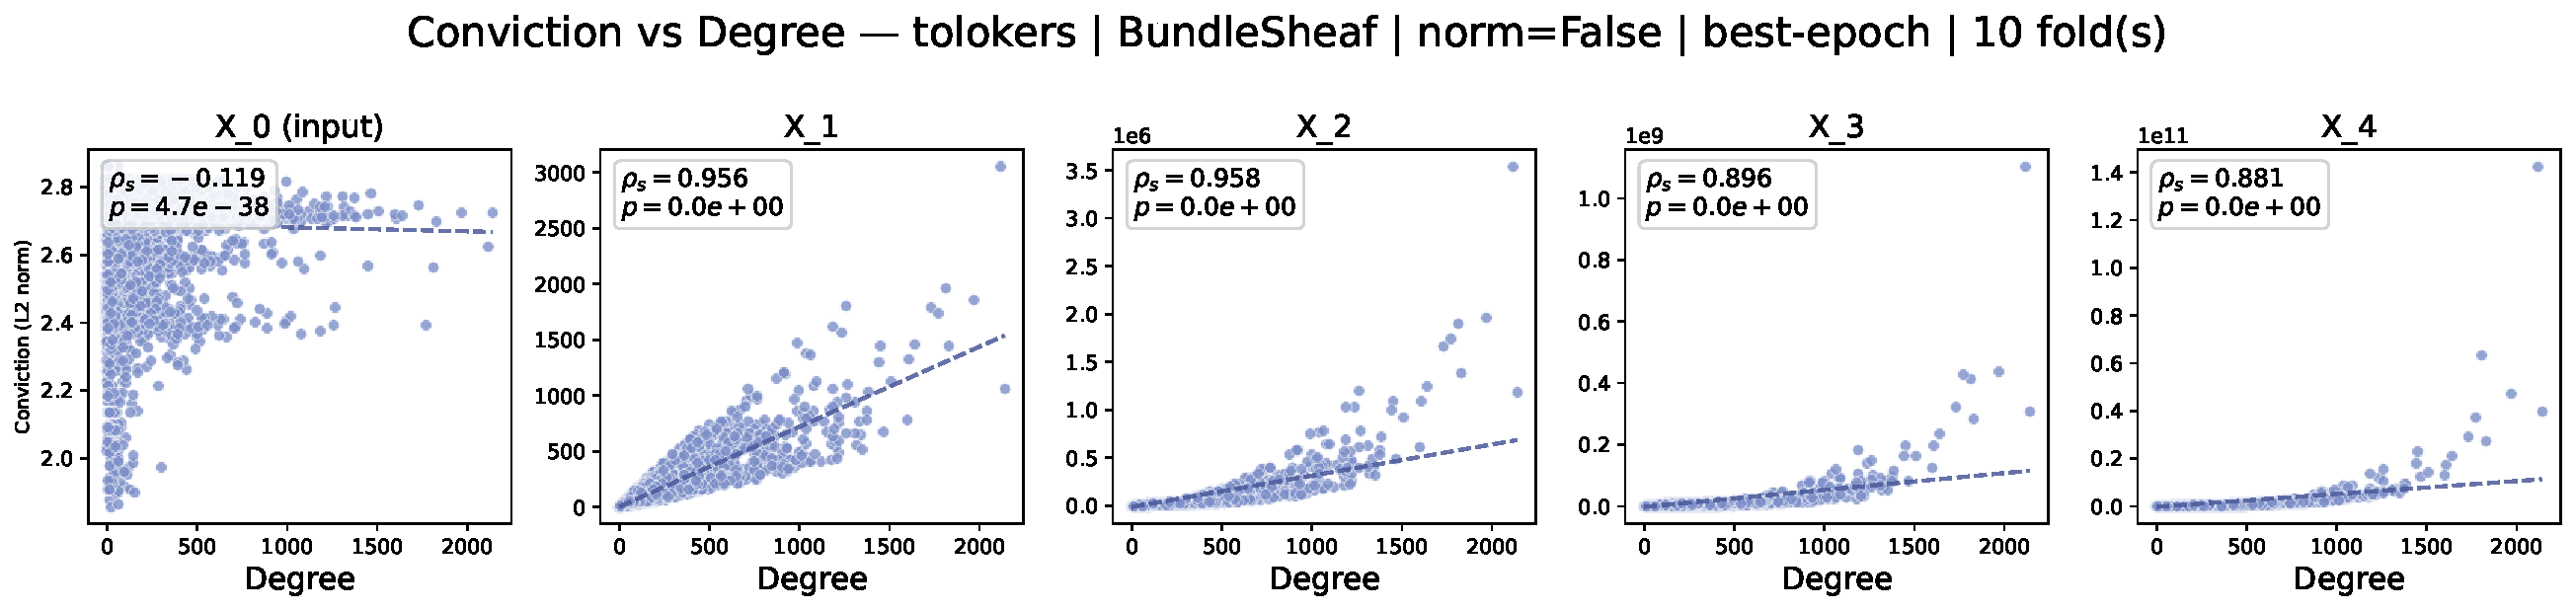
\includegraphics[width=\linewidth]{conviction_scatter/BundleSheaf/normalised_false/tolokers_BundleSheaf_d3_4L_Norm_False_conviction_scatter.pdf}
\end{figure}
\end{frame}

\begin{frame}{Wisconsin --- BundleSheaf, $d=2$, $L=2$, Norm=False}
\begin{figure}
    \centering
    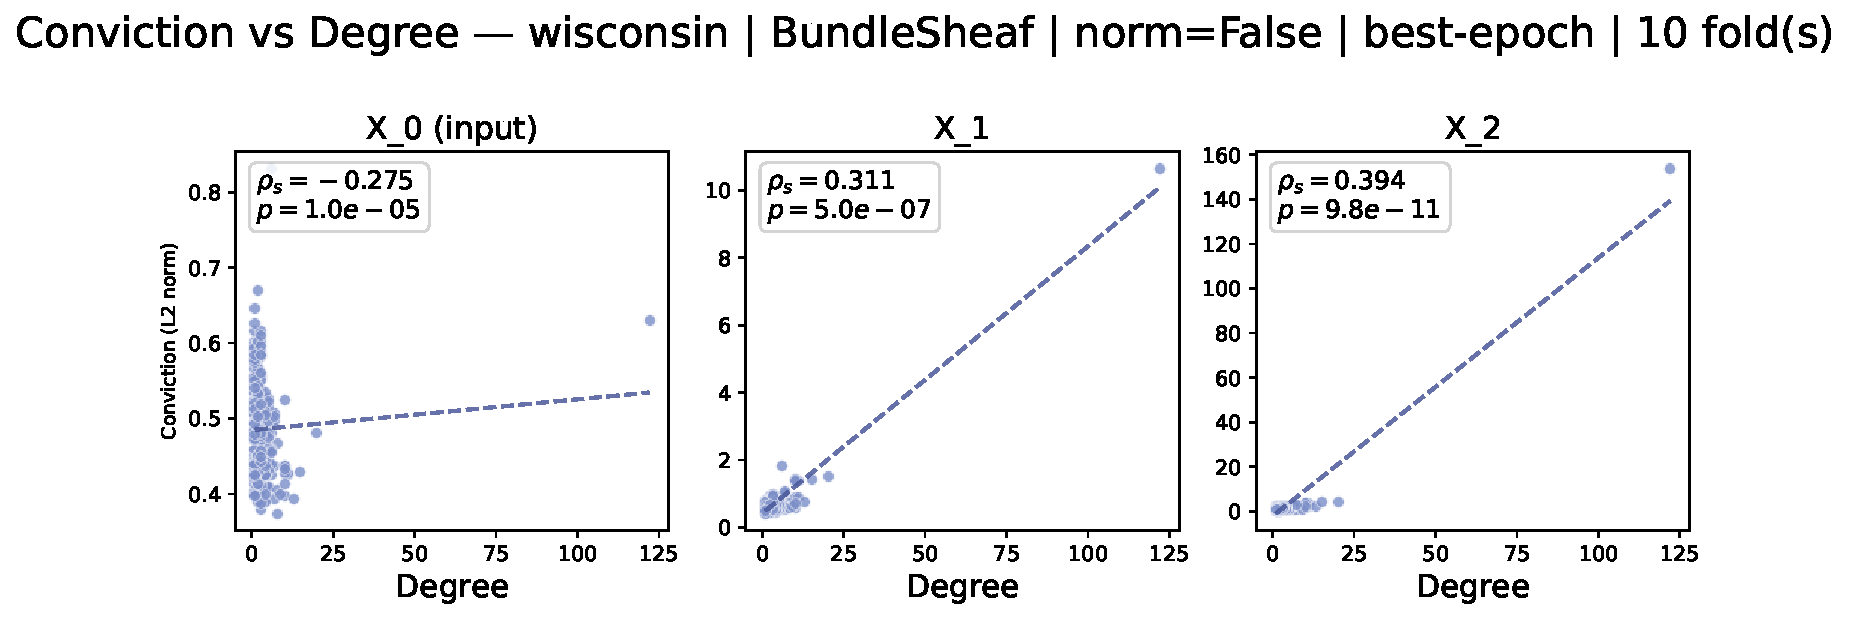
\includegraphics[width=0.8\linewidth]{conviction_scatter/BundleSheaf/normalised_false/wisconsin_BundleSheaf_d2_2L_Norm_False_conviction_scatter.pdf}
\end{figure}
\end{frame}


\end{document}
